\documentclass[12pt,a4paper]{book}%landscape,twocolumn,
\usepackage[spanish]{babel}
%\usepackage{fontspec}
%\usepackage{unicode-math}
%
%\setmainfont{Fira Sans}
%\setmathfont{Fira Math}
\usepackage{kpfonts}
\setlength{\parindent}{.5 cm}   %Activar sangrias

\usepackage[backend=biber, style=alphabetic]{biblatex}
\addbibresource{referencias.bib}
\usepackage{xcolor}
\usepackage{color}
\usepackage{float}
\usepackage{subcaption}
\usepackage{amsthm}
\usepackage{amsmath}
%\usepackage{amssymb}
\usepackage{hyperref}           % Enlaces y referencias internas
\usepackage{mathrsfs}           % Fuente caligráfica
\usepackage{wasysym}
\usepackage{fancyhdr}           % Encabezados y pies de página personalizados
\usepackage{tikz-cd}
\usepackage{tikz}
\usetikzlibrary{babel}
\usepackage{abc}
\usepackage{csquotes}


%\usepackage{geometry}
\usepackage[
a4paper,
top=2.54cm,
bottom=2.54cm,
left=2.54cm,
right=2.54cm
]{geometry}



%\usepackage{array, multirow, multicol}

%\usepackage{amsmath,amssymb,amsthm} % Paquetes de matemáticas
%\usepackage{amsfonts}           % Fuentes matemáticas adicionales

%
%%\usepackage{latexsym,url,colortbl,amsmath,amssymb,amsfonts,amsthm,mdframed,fancyhdr,lastpage}
%%\usepackage{paralist,etoolbox,enumerate,mathrsfs}
%%\usepackage[usenames,dvipsnames]{xcolor}
%%\pagestyle{fancy}\fancyhf{}
%%%\renewcommand{\headrulewidth}{0pt}}
%%%\spanishdecimal{.}
%%\pretolerance=2000
%%\tolerance=3000
%\usepackage{graphicx}
%%\counterwithin*{equation}{section}
%%\counterwithin*{equation}{subsection}
%%\renewcommand\theequation{\ifnumgreater{\value{subsection}}{0}{\thesubsection.}{\thesection.}\arabic{equation}}%
%



% Definición de entornos teorema, lema, etc.
%\theoremstyle{plain}
\newtheorem{theorem}{Teorema}[chapter]
\newtheorem{lemma}[theorem]{Lema}
\newtheorem{propo}[theorem]{Proposición}
\newtheorem{corollary}[theorem]{Corolario}

\theoremstyle{definition}
\newtheorem{definition}[theorem]{Definición}
\newtheorem{example}[theorem]{Ejemplo}
\theoremstyle{remark}
\newtheorem{remark}[theorem]{Observación}

\let\oldproofname=\proofname
\renewcommand{\proofname}{\rm\bf{Demostración}}
\renewcommand{\qedsymbol}{$\blacksmiley$}

\newcommand{\nn}{\mathbb{N}}
\newcommand{\rr}{\mathbb{R}}
\newcommand{\cc}{\mathbb{C}}
\newcommand{\zz}{\mathbb{Z}}
\newcommand{\pp}{\mathbb{P}}
\newcommand{\oo}{\mathscr{O}}
\newcommand{\afin}{\mathbb{A}}
\newcommand{\dom}{\mathrm{dom}}
\newcommand{\trdeg}{\mathrm{trdeg}}
\newcommand{\Der}{\mathrm{Der}}
\newcommand{\zn}{z_1,z_2,\dots,z_n}
\newcommand{\im}{\mathfrak{m}}

\title{\Huge \textbf{Notas de Geometría Compleja}} 
\author{\Large Héctor Gabriel Rodríguez Morales}
\date{}

\begin{document}
	
	\maketitle
	\thispagestyle{empty}  % Quitar el número de página en la portada
	\newpage
	
	\tableofcontents
	
	\newpage
	
	\listoffigures
	
	\newpage
	
	%\renewcommand{\listtablename}{Índice de tablas}
	%\listoftables
	
	%-----------------------new page----------------------------
	
	\mainmatter
	
%	\chapter*{Introducción}
\addcontentsline{toc}{chapter}{Introducción}
\pagenumbering{arabic}


\begin{quote}
	While the move from dimension 2 to dimension 3 appears to be the obvious step there is a sense in which one should move from 2 to 4. This comes from the consideration of complex algebraic geometry. For complex dimension 1 this theory was started by Abel and continued by Riemann. For algebraic varieties of complex dimension n the real dimension is 2n. The key figures in the topology of higher-dimensional algebraic varieties were Lefschetz, Hodgex, Cartan and Serre. While general algebraic geometry was one of the major developments of the second half of the 20th century, the topology of real 4-manifolds had a great surprise in store when Simon Donaldson made spectacular discoveries opening up an entirely new area.
	
	\hfill --- James Carlson, \textit{The Poincaré Conjecture}, AMS (2014)
\end{quote}


En la intersección entre el análisis complejo y la geometría diferencial surge una de las ramas más hermosas de la geometría; la \textit{geometría compleja}. Esta rama se encarga de estudiar objetos como variedades complejas, variedades algebraicas, funciones en varias variables, haces vectoriales holomorfos, entre otros. En particular, se hace un estudio profundo de objetos que generalizan las superficies de Riemann en dimensiones mayores; las variedades complejas. Este enfoque constituye un pilar para numerosas teorías contemporáneas, incluyendo la cohomología de Dolbeault y de gavillas, la teoría de Hodge, el estudio de foliaciones holomorfas, la teoría de singularidades y la teoría de cuerdas.

Una variedad compleja es un espacio que localmente se comporta como un abierto del espacio complejo $\cc^n$, pero cuyo comportamiento global puede ser mucho más profundo. Además, se encuentra equipado con funciones de transición holomorfas, lo cual garantiza una compatibilidad entre la geometría local compleja y todo el espacio. Sin embargo, la condición de holomorfia es más rígida que la suavidad real. Por ejemplo, las variedades complejas compactas no admiten funciones holomorfas globales no constantes, y el espacio de secciones globales de un haz vectorial holomorfo siempre tiene dimensión finita, en el caso compacto. La inexistencia de un teorema del encaje de Whitney general, sumado a fenómenos como el teorema de Hartogs, el comportamiento local de las funciones holomorfas y el concepto de funciones meromorfas, nos muestran una teoría esencialmente distinta a la geometría diferencial real. Por esta razón, buscamos herramientas más manejables para abordar las variedades complejas. Una diferencia importante respecto a las variedades suaves reales, y la cual es particularmente relevante para este trabajo, es la cercanía de las variedades complejas con las variedades algebraicas. En particular, estas conexiones con la geometría algebraica son recurrentes y una parte profunda de la teoría.

La \textbf{algebreización de variedades complejas} consiste, de manera informal, en asociar a una variedad compleja una variedad algebraica que la reproduzca como objeto analítico. Esto permite reemplazar un objeto analítico por uno algebraico, ganando acceso a herramientas mucho más rígidas, estructuradas y computacionales. Por ejemplo, en geometría algebraica, las funciones meromorfas del espacio proyectivo son cocientes de polinomios homogéneos del mismo grado. De este modo, podemos reemplazar las complejidades que conlleva la descripción holomorfa (continuidad, diferenciabilidad y convergencia) por problemas puramente algebraicos (ecuaciones polinomiales, estructuras algebraicas, invariantes algebraicos). De esta manera, \textit{algebrizar significa mostrar que la complejidad analítica está gobernada por su estructura algebraica subyacente}.

El objetivo del trabajo es presentar las propiedades básicas de las variedades complejas, incluyendo un estudio breve de las aplicaciones y funciones holomorfas, el concepto de gavilla sobre una variedad compleja, así como presentar ejemplos importantes de estos objetos. Posteriormente, se abordará el problema de encajar una variedad compleja a un espacio proyectivo, para lo cual se introduce el concepto de haz lineal y la idea de amplitud. En el último capítulo, entenderemos y demostraremos el teorema de Chow, apoyándonos en los resultados de Remmert. Este teorema será el eje central de todo el trabajo, pues conecta todos los conceptos estudiados. Finalmente, en las dos últimas secciones vamos a presentar brevemente los conceptos de variedad de Moishezon y Kähler, con el propósito de entender su importancia en el tema de la algebrización. 

A lo largo del trabajo se asumirá familiaridad con los fundamentos de topología general y análisis complejo en una variable. Sin embargo, se incluye un apéndice con resultados sobre funciones holomorfas de varias variables que serán citados a lo largo de todo el trabajo. Asimismo, se hará referencia durante todo el trabajo a conceptos y resultados clásicos del álgebra conmutativa, geometría algebraica y superficies de Riemann, remitiendo al lector a la bibliografía clásica y citando únicamente aquellos resultados técnicos que sean necesarios. Para las dos últimas secciones se utilizarán nociones más avanzadas de la geometría algebraica y geometría diferencial. Así, dichos temas solo serán presentados de manera breve y no se hará un desarrollo exhaustivo.


	
	%-----------------------new page----------------------------
	
	\chapter{Álgebra Conmutativa}
En este trabajo, todos los anillos los consideramos anillos conmutativos con unidad, y los morfismos de anillos mapean el uno al uno.

\section{Generalidades}

\begin{definition}[$A$-módulo]
    Sea $A$ un anillo y $M$ un grupo abeliano. Decimos que $M$ es un \textbf{$A$-módulo} (izquierdo) si existe una operación $\cdot:A\times M\to M$ tal que para todo $a,b\in A$ y $m,n\in M$ se cumple que: 
    \begin{enumerate}
        \item $a\cdot (m+n)=a\cdot m+a\cdot n$
        \item $(a+b)\cdot m=a\cdot m + b\cdot m$
        \item $(ab)\cdot m=a(b\cdot n)$
        \item $1\cdot m=m$
    \end{enumerate}
\end{definition}

Se define $A$-módulo derecho de forma análoga, sin embargo, ambas estructuras coinciden ya que $A$ es un anillo conmutativo. Por lo que no haremos distinción sobre los $A$-módulos izquierdo y derechos para llamarlos simplemente \textit{$A$-módulos}.

\begin{definition}[$A$-álgebra]
    Sean $A$ y $B$ dos anillos. Decimos que $B$ es un \textbf{$A$-álgebra} si $B$ es un $A$-módulo. Equivalentemente, si existe 
    morfismo de anillos $f:A\to B$ no cero. Este morfismo induce una estructura de $A$-módulo a $B$ de la siguiente forma
    \begin{align*}
        \cdot:A\times B\to B\\
        a\cdot b:=f(a)b
    \end{align*}
\end{definition}

\begin{definition}[Morfismo de álgebras]
    Sean $A$ y $A'$ dos $B$-álgebras. Entonces, existen morfismos de anillos $f:B\to A$ y $f':B\to A'$. Un \textbf{morfismo de $B$-álgebras} es un morfismo de anillos $\phi:A\to A'$ tal que el siguiente diagrama conmuta
    \begin{center}
        \begin{tikzcd}
	& B \\
	\\
	A && {A'}
	\arrow["f"', from=1-2, to=3-1]
	\arrow["{f'}", from=1-2, to=3-3]
	\arrow["\phi"', from=3-1, to=3-3]
\end{tikzcd}
    \end{center}
\end{definition}

\begin{definition}
    Sea $A$ un anillo. Decimos que un $A$-módulo $M$ es \textbf{finitamente generado} (o \textbf{finito}) si existen elementos $m_1,\dots,m_n\in M$ tal que
    \begin{equation*}
        M=\mathrm{gen}_A\{m_1,\dots,m_n\}=\left\{\sum_{i=1}^n a_im_i: a_i\in A \right\}
    \end{equation*}
    Equivalentemente, $M$ es finito si es isomorfo a $n$ copias de $A$
    \begin{equation*}
    	M\cong\bigoplus_{i=1}^n A.
    \end{equation*}
    Decimos que una $A$-álgebra $B$ es \textbf{finitamente generada} como $A$-álgebra (o de \textbf{tipo finito}) si existe un morfismo de $A$-álgebras sobreyectivo
    \begin{center}
        \begin{tikzcd}
	{A[x_1,\dots,x_n]} && B && 0
	\arrow["\phi", from=1-1, to=1-3]
	\arrow[from=1-3, to=1-5]
\end{tikzcd}
    \end{center}
    
\end{definition}


    Notemos de inmediato que si una $A$-álgebra es finitamente generado como $A$-módulo, entonces es de tipo finito pues está generado por polinomios lineales.
    
    \begin{example}
    	Supongamos que $M$ es un $A$-álgebra finitamente generada como $A$-módulo. Consideremos el morfismo $\phi:A[x_1,\dots,x_n]\to M$ dado por
    	\begin{equation*}
    		\phi(f(x_1,dots,x_n))=f(m_1,\dots,m_n).
    	\end{equation*}
    	Como $M$ es finito, entonces existe un conjunto generador finito $\{m_1,\dots,m_n\}\subset M$. Así, para todo $m\in M$ existen $a_1,\dots,a_n\in A$ tal que
    	\begin{equation*}
    		m=a_1m_1+\dots+a_nm_n.
    	\end{equation*} 
    	Esto implica que 
    	\begin{equation*}
    		m=\phi(a_1x_1+\dots+a_nx_n).
    	\end{equation*}
    	Por lo tanto, $\phi$ es un morfismo sobreyectivo. Es decir, $M$ es un $A$-álgebra de tipo finito.
    \end{example}
    
    \begin{remark}
    	Sea $B$ una $A$-álgebra de tipo finito. Entonces existe un morfismo sobreyectivo
    	\begin{equation*}
    		f:A[x_1,\dots,x_n]\longrightarrow B.
    	\end{equation*}
    	Por el primer teorema de isomorfía,
    	\begin{equation*}
    		B\cong A[x_1,\dots,x_n]/\ker(f).
    	\end{equation*}
    	Conversamente, si $B\cong A[x_1,\dots,x_n]/I$ para algún ideal $I\subset A[x_1,\dots,x_n]$. Entonces el morfismo canónico
    	\begin{align*}
    		f:A[x_1,\dots,x_n]&\longrightarrow A[x_1,\dots,x_n]/I\cong B\\
    		&\alpha\mapsto [\alpha]
    	\end{align*}
    	es sobreyectivo con kernel $\ker(f)=I$. Así, $B$ es una $A$-álgebra de tipo finito. Por lo tanto
    	\begin{center}
    		\textbf{$B$ de una $A$-álgebra de tipo finito si, y solo si, $B$ es isomorfo como $A$-álgebra a un anillo cociente $A[x_1,\dots,x_n]/I$ para algún ideal $I\subset A[x_1,\dots,x_n]$.}
    	\end{center}
    \end{remark}
    
    
    \begin{definition}
    	Decimos que un morfismo de anillos $f:A\to B$ es un \textbf{morfismo finito} si $B$ es un $A$-módulo finito. Análogamente, decimos que $f$ es un \textbf{morfismo de tipo finito} si $B$ es una $A$-álgebra de tipo finito.
    	Por último, decimos que $f$ es un \textbf{morfismo de presentación finita} si es de tipo finito y el ideal asociado a $B$ es finitamente generado, es decir, existen $f_1,\dots,f_k$ polinomios tal que
    	\begin{equation*}
    		B\cong A[X_1,\dots,x_n]/\langle f_1,\dots,f_k\rangle.
    	\end{equation*}
    \end{definition}
    
    \begin{example}[Anillo de números duales]
    	Consideremos el anillo
    	\begin{equation*}
    		B=\cc[\epsilon]/\langle \epsilon^2\rangle.
    	\end{equation*}
   
		Notemos que los elementos de $B$ son de la forma,
    	\begin{equation*}
    		a+b\epsilon,\qquad a,b\in\cc,\qquad \epsilon^2=0.
    	\end{equation*}
    	Este anillo satisface varias propiedades importantes.
    	\begin{itemize}
    		\item Es un $\cc$-espacio vectorial de dimensión $2$ con base $\{1,\epsilon\}$. Esto quiere decir que el morfismo natural
    		\begin{equation*}
    			f:\cc\longrightarrow \cc[\epsilon]/\langle \epsilon^2\rangle,
    		\end{equation*}
    		es finito.
    		\item No es dominio entero porque $\epsilon\cdot\epsilon=0$.
    		\item Un elemento es invertible si, y solo si, $a\neq 0$. Esto debido a que
    		\begin{equation*}
    			(a+b\epsilon)^{-1}=\frac{1}{a}-\frac{b}{a^2}\epsilon.
    		\end{equation*}
    		Por lo que, el ideal $\langle \epsilon \rangle$ contiene todos lo elementos no invertible y por lo tanto, es el único ideal maximal de $B$. Es decir, $B$ es un anillo local.
    		\item El campo residual de $B$ es
    		\begin{equation*}
    			\frac{\cc[\epsilon]/\langle \epsilon^2\rangle}{\langle \epsilon \rangle}\cong\cc.
    		\end{equation*}
    		\item El anillo $B$ es un anillo artiniano, y en consecuencia, $B$ es noetheriano.
    	\end{itemize}
    \end{example}
    
    
 \section{Espectro primo de un anillo}
 
 
 \section{Dimensión de un anillo}
    
    Ahora introduzcamos una noción de dimensión para cualquier anillo.
\begin{definition}
    Sea $A$ un anillo. La \textcolor{blue}{altura} $\mathrm{ht}$ de un ideal primo $\mathfrak{p}\subset A$ es el supermo de todos $n$ de las cadenas
    \begin{equation*}
        \langle 0 \rangle= \mathfrak{p}_0\subset \mathfrak{p}_1\subset \cdots \subset \mathfrak{p}_n= \mathfrak{p}
    \end{equation*}
    Definimos la \textcolor{blue}{dimensión de Krull} como el número
    \begin{equation*}
        \mathrm{dimkrull}(A)=\sup_{\mathfrak{p}\text{ primo}}\mathrm{ht}(\mathfrak{p})
    \end{equation*}
\end{definition}

    \begin{theorem}\label{krulltrdeg}
        Sea $k$ un campo y $B$ dominio entero finitamente generado como $k$-álgebra.
        \begin{enumerate}
            \item Si $Q(B)$ es el campo de fracciones asociado al dominio entero $B$, entonces
            \begin{equation*}
                \mathrm{trdeg}_kQ(B)=\mathrm{dimkrull} B
            \end{equation*}
            \item Para cualquier ideal primo $\mathfrak{p}\subset B$ se cumple que
            \begin{equation*}
                \mathrm{dimkrull} B = \mathrm{ht}(\mathfrak{p}) + \mathrm{dimkrull} B/\mathfrak{p}
            \end{equation*}
        \end{enumerate}
    \end{theorem}

    \begin{corollary}
        Si $k$ un campo, entonces la dimensión de Krull del anillo de polinomio $k[x_1,\dots, x_n]$ es $n$.
    \end{corollary}
    \begin{proof}
        Solo es suficiente notar que $k[x_1,\dots, x_n]$ trivialmente una $k$-álgebra de tipo finito y
        \begin{equation*}
            \mathrm{trdeg}_kQ(k[x_1,\dots, x_n])=\mathrm{trdeg}_k k(x_1,\dots, x_n)=n
        \end{equation*}
        Por el teorema anterior
        \begin{equation*}
            \mathrm{dimkrull}k[x_1,\dots, x_n]=n
        \end{equation*}
    \end{proof}

    \begin{definition}
        Sea $\mathfrak{p}$ un ideal primo de $A$ e $I\subset A$ un ideal contenido en $\mathfrak{p}$. Decimos que $\mathfrak{p}$ es minimal sobre $I$ si no existe otro ideal primo $\mathfrak{q}$ tal que
        \begin{equation*}
            I\subsetneq \mathfrak{q}\subsetneq \mathfrak{p}
        \end{equation*}
    \end{definition}
    
    \begin{theorem}[del ideal principal de Krull]\label{principalkrull}
        Sea $A$ un anillo noetheriano y $f\in A$ un elemento no unidad ni divisor de cero. Entonces todo ideal primo minimal sobre $\langle f \rangle$ tiene altura $1$.
    \end{theorem}

    \begin{propo}\label{dfuprincipal}
        Sea $A$ un dominio entero noetheriano. Entonces $A$ es DFU si, y solo si, todo ideal primo de altura $1$ es principal.
    \end{propo}

    \begin{lemma}\label{lemaisoresidual}
        Sea $A$ un anillo y $\mathfrak{p}$ un ideal primo de $A$, entonces $A_\mathfrak{p}$ un anillo local con ideal maximal
        \begin{equation*}
            \mathfrak{p}A_\mathfrak{p}:=\left\{\frac{a}{s}\in A_\mathfrak{p}:a\in \mathfrak{p}\right\}
        \end{equation*}
        Además, existe un isomorfismo entre el campo residual $\kappa(\mathfrak{p})=A_\mathfrak{p}/\mathfrak{p}A_\mathfrak{p}$ y el campo de fracciones del dominio entero $A/\mathfrak{p}$
    \end{lemma}

    \begin{theorem}[de la base de Hilbert]\label{basehilbert}
    	Si $A$ es un anillo noetheriano, entonces $A[X_1,\dots, X_n]$ también es un anillo noetheriano.
    \end{theorem}
    
    \subsection{Anillo noetheriano con dimensión infinita}
    
    A continuación, presentaremos un ejemplo de \textit{Nagata}, el cual es un anillo noetheriano de dimensión infinita. Cabe destacar que dicho anillo no puede ser local.
    
    
\section{Álgebra de series formales}

\begin{definition}
    Sea $A$ un anillo. Una \textbf{serie formal de potencias} con coeficientes en $A$ es un mapeo
    \begin{align*}
        \mathrm{N}^n\to A\\
        \alpha\mapsto c_\alpha
    \end{align*}
    donde $c_\alpha\in A$. Este mapeo se denota por el simbolo
    \begin{equation*}
        \sum_{\alpha\in\mathrm{N}^n}c_{\alpha}z^{\alpha}
    \end{equation*}
    donde $z=(\zn)$ donde $\zn$ son variables indeterminadas sobre $A$. El conjunto de todas las series formales de potencias con coeficientes en $A$ se denota por
    \begin{equation*}
        A[[\zn]]
    \end{equation*}
    Una serie formal de potencias $f=\sum_{\alpha\in\mathrm{N}^n}c_{\alpha}z^{\alpha}$ tiene un \enquote{valor en el cero} bien definido
    \begin{equation*}
        f(0):=c_{0,\dots,0}
    \end{equation*}
\end{definition}

\begin{theorem}
    Sea $A$ un anillo y $k$ un campo. Entonces se cumple lo siguiente:
    \begin{enumerate}
        \item $A[[\zn]]$ es un anillo con las siguientes operaciones
        \begin{align*}
            \sum_{\alpha\in\mathrm{N}^n}a_{\alpha}X^{\alpha}+\sum_{\alpha\in\mathrm{N}^n}b_{\alpha}X^{\alpha}:=\sum_{\alpha\in\mathrm{N}^n}(a_{\alpha}+b_\alpha)X^{\alpha}\\
            \left(\sum_{\alpha\in\mathrm{N}^n}a_{\alpha}X^{\alpha}\right)\cdot\left(\sum_{\beta\in\mathrm{N}^n}b_{\beta}X^{\beta}\right):=\left(\sum_{\gamma\in\mathrm{N}^n}c_{\gamma}X^{\gamma}\right)
        \end{align*}
        donde 
        \begin{equation*}
            c_\gamma:=\sum_{\alpha+\beta=\gamma}a_\alpha b_\beta
        \end{equation*}
        Más aún, si $A$ es una $k$-álgebra  entonces $A[[\zn]]$ también es una $k$-álgebra con la operación
        \begin{equation*}
        \lambda\cdot\sum_{\alpha\in\mathrm{N}^n}a_{\alpha}X^{\alpha}:=\sum_{\alpha\in\mathrm{N}^n}(\lambda\cdot a_{\alpha})X^{\alpha}
        \end{equation*}
        
    \item $A[[\zn]]$ contiene al anillo de polinomios (álgebra) $A[\zn]$ como un subanillo (subalgebra).

    \item 
    \begin{align*}
        A[[z_1,z_2,\dots,z_n]]&=(A[[z_1,z_2,\dots,z_{n-1}]])[[z_n]]\\
        &=\cdots=((A[[z_1]])\dots [[z_n]])
    \end{align*}
    
    \item Si $A$ es un anillo noetheriano, entonces $A[[\zn]]$ también es un anillo noetheriano.

    \item Si $A=k$ es un campo, entonces $k[[\zn]]$ es un DFU. 
    \end{enumerate}    
\end{theorem}

Recordemos que los números complejos vienen equipados con una norma llamada módulo $|\cdot|:\cc^n\to \rr_{\geq 0}$ dada por la norma euclidiana de $\rr^{2n}$. Vamos a darle una norma al anillo de series formales con este módulo.

Para cada $r\in\rr_{>0}^n$, definimos el mapeo
	\begin{equation*}
		\|\cdot\|_r:\cc[[\zn]]\longrightarrow \rr_{\geq 0}\cup\{\infty\}
	\end{equation*}
dado por
\begin{equation*}
	\|f\|_r:=\sum_{\alpha\in\nn^n} |c_\alpha|r^\alpha\in\rr_{\geq 0}\cup\{\infty\}.
\end{equation*}
Notemos que $\|\cdot\|_r$ es una norma sobre el conjunto de series de potencias $f$ con $\|f\|_r<\infty$.

\begin{definition}
	Sea $f=\sum_{\alpha\in\mathbb{N}^{n}}c_\alpha z^{\alpha}\in \cc[[\zn]]$ una seria forma de potencias. Decimos que $f$ \textbf{converge} si existe un vector real $r\in \rr_{>0}^n$ tal que
		\begin{equation*}
			\|f\|_r<\infty.
		\end{equation*}
	Equivalentemente que
	\begin{equation*}
		\sup_{\alpha\in\mathbb{N}^{n}}|c_\alpha|r^\alpha<\infty.
	\end{equation*} 
\end{definition}

Esta condición nos dice que para que una serie converja, su crecimiento debe ser a lo más exponencial.

\begin{example}
	Cualquier polinomio en $\cc[\zn]$ converge pero no toda serie forma de potencias converge. Por ejemplo, consideremos la serie
	\begin{equation*}
		f=\sum_{n=0}^{\infty} n!z^n.
	\end{equation*} 
	Supongamos que existe $r>0$ tal que
	\begin{equation*}
		\sup_{n\in\nn}n!r^n<\infty.
	\end{equation*}
	
\end{example}
\begin{definition}
    El conjunto de las \textbf{series convergente} (en el cero) es el conjunto definido por
    \begin{align*}
    	\cc\{\zn\}:=&\{f\in\cc[[\zn]]:\text{ existe }r\in \rr_{>0}^n\text{ tal que }\|f\|_r<\infty\}\\
    	=&\left\{\sum_{\alpha\in\mathbb{N}^{n}}c_\alpha z^{\alpha}:\text{existe }r\in\rr^n_{\geq 0}\text{ tal que }\sup_{\alpha\in\mathbb{N}^{n}}|c_\alpha| r^{\alpha}<\infty \right\}
    \end{align*}
\end{definition}

\begin{remark}
    Notemos que tenemos una cadena estricta de subalgebras
    \begin{equation*}
        \cc[z_1,\dots,z_n]\subsetneq\cc\{z_1,\dots,z_n\}\subsetneq\cc[[z_1,\dots,z_n]]
    \end{equation*}
    Además, sabemos que podemos definir una serie convergente en un punto $a=(a_1,\dots,a_n)$ y obtener el conjunto $\cc\{z_1-a_1,\dots,z_n-a_n\}$. Sin embargo, es inmediato que
    \begin{equation*}
        \cc\{z_1-a_1,\dots,z_n-a_n\}\cong 
        \cc\{z_1,\dots,z_n\}
    \end{equation*}
\end{remark}

\begin{definition}
    Sea $f=\sum_{\alpha\in\mathbb{N}^n}c_\alpha z^{\alpha}\in\cc[[z_1,\dots,z_n]]$ una serie formal de potencias. El \textcolor{blue}{orden} (o subgrado) de $f$ esta definido por
    \begin{equation*}
        \mathrm{ord}(f)=\begin{cases}
            \infty &,\text{ si }f\\
            \min\{|\alpha|:c_\alpha\neq 0\} &,\text{ si }f\neq 0
        \end{cases}
    \end{equation*}
\end{definition}

\begin{example}
    Consideremos la serie
    \begin{align*}
        f(z_1,z_2)&=z_1^4+z_2\sin(z_1z_2)\\
        &=z_1^4+z_2\sum_{k\geq 1}\frac{(-1)^k}{(2k+1)!}(z_1z_2)^{2k+1} \\
    \end{align*}
    Entonces
    \begin{equation*}
        \mathrm{ord}(f)=3
    \end{equation*}
\end{example}

\begin{lemma}
    Sea $f,g\in \cc[[z_1,\dots,z_n]]$. Entonces se cumple que:
    \begin{enumerate}
        \item El orden satisface que
        \begin{align*}
            \mathrm{ord}(f+g)\geq \min\{\mathrm{ord}(f),\mathrm{ord}(g)\}\\
            \mathrm{ord}(fg)=\mathrm{ord}(f)+\mathrm{ord}(g)\\
        \end{align*}
        \item El álgebra $\cc[[z_1,\dots,z_n]]$ es un dominio entero.
        \item $f\in  \cc[[z_1,\dots,z_n]]$ es unidad si, y solo si, $\mathrm{ord}(f)=0$.
    \end{enumerate}
\end{lemma}

\begin{propo}
    El anillo $\cc[[z_1,\dots,z_n]]$ es un anillo local. Es decir, el conjunto de todos los elementos no unidad
    \begin{equation*}
        \mathfrak{m}=\{f\in  \cc[[z_1,\dots,z_n]]:f(0)=0\}
    \end{equation*}
    es un ideal. Más aún, es un ideal máximal, es único y está generado por $z_1,\dots,z_n$.
\end{propo}

\section{Teorema de los ceros de Hilbert}

Un morfismo de anillos $f:A\to B$ se llama \textbf{integral} si para todo elementos $b\in B$ es integral sobre $A$, es decir, existe un polinomio mónico $\sum_{i=1}^na_ix^i\in A[x]$ tal que
\begin{equation*}
	\sum_{i=1}^{n}f(a_i)b^i=0.
\end{equation*}
Esta ecuación es llamada \textbf{ecuación integral} de $b$ sobre $A$. 

\begin{propo}
	Sea $f:A\to B$ un morfismo de anillo. Entonces $f$ es finito si, y solo si, es integral y de tipo finito.
\end{propo}
\begin{proof}
	Supongamos que $f:A\to B$ es finitamente generado como $A$-módulo con la estructura inducida por $f$. Claramente, $f:A\to B$ también es de tipo finito. 
\end{proof}


\begin{theorem}[Lema de normalización de Noether]
	Sea $A$ una $k$-álgebra de tipo finito. Entonces existe un entero $d\geq 0$ y un morfismo inyectivo finito $k[x_1,\dots,x_d]\hookrightarrow A$.
\end{theorem}


\begin{corollary}
	Sea $k$ un campo e $I$ un ideal propio de $k[x_1,\dots, x_n]$. Entonces existe una sub-algebra $k[s_1,\dots,s_n]$ de $k[x_1,\dots,x_n]$ y un entero $0\leq r\leq n$ tal que:
	\begin{enumerate}
		\item $k[x_1,\dots,x_n]$ es finito sobre $k[s_1,\dots,s_n]$.
		\item $k[s_1,\dots,s_n]\cap I=\langle s_1,\dots,s_n\rangle$.
		\item $k[s_{r+1},\dots,s_n]\to k[x_1,\dots,x_n]/I$ es finito e inyectivo. 
	\end{enumerate}
\end{corollary}

\begin{corollary}
	Sea $A$ una $k$-álgebra de tipo finito. Sea $\im$ un ideal maximal de $A$, entonces $A/\im$ es una extensión finita algebraica de $k$.
\end{corollary}

\begin{corollary}[Teorema de los ceros débil]
	Sea $k$ un campo algebraicamente cerrado. Entonces para cualquier ideal maximal $\im$ de $k[x_1,\dots,x_n]$ existe un único punto $(a_1,\dots,a_n)\in k^n$ tal que
	\begin{equation*}
		\im=\langle x_1-a_1,\dots,x_n-a_n\rangle.
	\end{equation*}
\end{corollary}

\begin{lemma}
	Sea $A$ una $k$-álgebra de tipo finito no cero. Entonces la intersección de todos los ideales maximales de $A$ es igual al nilradical de $A$.
\end{lemma}

\begin{theorem}
	Sea $k$ un campo algebraicamente cerrado e $I$ un ideal de $k[x_1,\dots,x_n]$. Si $f\in k[x_1,\dots,x_n]$ es un polinomio tal que 
	\begin{equation*}
		F(\alpha)=0,\qquad \text{para todo }\ \alpha\in Z(I),
	\end{equation*}
	entonces $f\in \sqrt{I}$.
\end{theorem}

\chapter{Geometría Local}
\section{Funciones holomorfas de varias variables}

No es objetivo indagar demasiado en el estudio de las funciones complejas en varias variables. Sin embargo, es necesario presentar el concepto de holomorfia para definir una variedad compleja. La mayoria de resultados se pueden encontrar en \parencite[Cap 1, Sec 1.1]{huybrechts2005complex}\\
Fijemos $U\subset\cc^n$ un subconjunto abierto. Para cualquier $w\in U$, definimos el \textbf{polidisco} como el conjunto definido por
\begin{equation*}
	B_\epsilon(w):=\{z: |z_i-w_i|<\epsilon_i\},\enspace \text{donde}\enspace \epsilon=(\epsilon_1,\epsilon_2,\cdots,\epsilon_n)
\end{equation*}

\begin{definition}[Función holomorfa]\label{taylor}
	Una función $f:U\subset \cc^n\to\cc$ es llamada holomorfa en un punto $w\in U$, si existe un polidisco $B_\epsilon(w)\subset U$ tal que la restricción $f\left.\right|_{B_\epsilon(w)}$ está dada por una serie de potencias convergente \begin{equation*}
		\sum_{(i_1,i_2,\cdots,i_n)\in\nn^n}^{\infty}a_{i_1,i_2,\cdots,i_n}(z_1-w_1)^{i_1}(z_2-w_2)^{i_2}\dots(z_n-w_n)^{i_n}
	\end{equation*}
	y es única.
\end{definition}

\begin{remark}[Definiciones equivalentes de holomorfia] Sea $f:U\to\cc$ una función. Entonces $f$ es holomorfa si 
	\begin{enumerate}
		\item Satisface las ecuaciones de Cauchy-Riemann en todas las coordenadas $z_j=x_j+iy_j$, es decir,
		\begin{equation*}
			\frac{\partial f}{\partial \overline{z_j}}=0,\qquad j=1,2,\cdots n
		\end{equation*}
		donde $\frac{\partial}{\partial \overline{z_j}}=\frac{1}{2}(\frac{\partial}{x}+i\frac{\partial }{\partial y})$.
		
		\item Es continuamente diferenciable y para todo $z\in U$ se cumple la siguiente fórmula
		\begin{equation*}
			f(z)=\frac{1}{(2\pi i)^n}\int_{\partial B_\epsilon(w)}\frac{f(w)}{(z_1-w_1)\dots(z_n-w_n)}dw_1\cdots dw_n
		\end{equation*}
	\end{enumerate}
	
\end{remark}

Veamos las generalizaciones de los resultados básico en una variable.

\begin{theorem}[Principio del máximo]\label{Principiodelmodulomaximo}
	Sea $U\subset \cc^n$ un conjunto abierto y conexo. Si $f:U\to\cc$ es una función holomorfa no constante, entonces $|f|$ no tiene un máximo local en $U$.
\end{theorem}

\begin{theorem}[de la identidad]\label{identidad}
	Sea $U\subset \cc^n$ un subconjunto abierto y conexo. Si $f,g:U\to \cc$ son funciones holomorfas tales que $f(z)=g(z)$ para todo $z$ es un abierto no vacio de $U$, entonces $f=g$.
\end{theorem}

\begin{theorem}[de Lioville]
	Toda función $f:\cc^n\to\cc$ holomorfa acotada es constante.  
\end{theorem}

\begin{theorem}[Hartogs]\label{hartogs}
	Sea $\Omega\subset\cc^n$ con $n\geq 2$ un dominio y $K\subset\Omega$ un subconjunto compacto tal que $\Omega\setminus K$ es también conexo. Entonces, toda función holomorfa $f:\Omega\setminus K\to\cc$ se extiende holomorfamente a todo $\Omega.$
\end{theorem}


\begin{definition}\label{mapholocn}
	Una función $f:U\to\cc^m$ es llamada \textbf{aplicación holomorfa} si todas las funciones coordenadas $f_1,\dots,f_m:U\to\cc$ son funciones holomorfas.
\end{definition}


\begin{definition}
	Sean $U,V\subset \cc^n$ dos abiertos no vacios. Un aplicación holomorfa $f:U\to V$ es \textbf{biholomorfa} si es biyectiva y su inversa $f^{-1}$ también es una aplicación holomorfa. Además decimos que $U$ y $V$ son biholomorfos. 
\end{definition}

El caso del teorema del mapeo de Riemann es un caso que no se puede extender a más dimensiones y es exclusivo para $n=1$.
\begin{theorem}
	Sea $B_1^n(0)=\{z\in\cc^n: \|z\|<1\}$ la bola euclidiana unitaria y $P_1^n(0)=\{z\in\cc^n:|z_i|<1,\text{ para cada }i=1,2,\cdots, n\}$ el polidisco unitario en $\cc^n$. Entonces $B_1^n(0)$ y $P_1^n(0)$ son biholomorfos si, y solo si, $n=1$. La demostración se encuentra en \parencite[Teo 3.9, Pg. 78]{scheidemann}
\end{theorem}


\begin{definition}\label{puntoregular}
	Sean $U\subset \cc^m$ un conjunto abierto y $f:U\to\cc^n$ una aplicación holomorfa. El \textbf{jacobiano} (complejo) de $f$ en un punto $z\in U$ es la matriz 
	\begin{equation*}
		J(f)(z):=\left(\frac{\partial f_i}{\partial z_j}(z) \right)_{i,j}
	\end{equation*}
	Un punto $z\in U$ es llamado \textbf{regular} si el rango de la matriz jacobiana $J(f)(z)$ es $n$. Si todo punto $z\in f^{-1}(w)$ es regular, decimos que $w$ es un \textbf{valor regular}.
\end{definition}



\begin{theorem}[Teorema de la función inversa]
	Sea $f:U\to V$ una aplicación holomorfa entre dos subconjuntos abiertos $U,V\subset \cc^n$ y $z\in U$. Entonces los siguiente enunciados son equivalentes:
	\begin{enumerate}
		\item $\det J(f)(z)\neq 0$
		\item Existen vecindades $z\in U'\subset U$ y $f(z)\in V'\subset V$ tal que 
		\begin{equation*}
			f\left.\right|_{U'}:U'\to V'
		\end{equation*}
		es un biholomorfismo.
	\end{enumerate}
\end{theorem}

\begin{theorem}[Teorema de la función implícita]\label{funcionimplicita}
	Sea $U\subset\cc^{n+m}$ un abierto y $f:U\to \cc^n$ una aplicación holomorfa en $U$. Si $(w_0,z_0)\in U$ es un punto tal que
	$$ \det\left(\frac{\partial f_i}{\partial z_j}(w_0,z_0)\right)_{1\leq i,j \leq n}\neq 0$$
	Entonces existe una vecindad $W\subset \cc^m$ de $w_0$, una vecindad de $Z\subset\cc^n$ de $z_0$ y una aplicación holomorfa $g:W\to Z$ tal que $f(w,g(w))=0$ para todo $w\in W$ y
	\begin{equation*}
		\{(w,z)\in U':f(w,z)=0\}=\{(w,g(w))\in U:w\in W\}
	\end{equation*}
\end{theorem}



\begin{propo}\label{biholomorfismojac}
	Sea $f:U\to V$ una aplicación holomorfa biyectiva entre dos subconjuntos abiertos $U,V\subset \cc^n$. Entonces para todo $z\in U$ se tiene que $\det J(f)(z)\neq 0$. En particular, $f$ es un biholomorfismo.
\end{propo}

\section{Comportamiento local}\label{complocal}

En una variable compleja, el comportamiento local de las funciones holomorfas es muy simple. Si $f:U\to\cc$ es una función holomorfa en alguna vecindad $U\subset\cc$ del cero, entonces $f$ se escribe de forma única como
\begin{equation*}
	f(z)=u(z)z^k
\end{equation*} 
para algún $k\in\nn$ y una función $u\in\mathscr{O}_n(U)$ unidad. Esto significa que $u(0)\neq 0$ y $1/u(z)$ está bien definida en alguna vecindad del cero. En varias variables complejas la situación es mucho más complicada.\\
\begin{definition}
	Sean $U,V\subset \cc^n$ vecindades del $0\in\cc^n$. Decimos que $f\in\mathscr{O}_n(U)$ y $g\in\mathscr{O}_n(V)$ están relacionadas si existe una vecindad $W\subset\cc^n$ del $0$ tal que
	\begin{equation*}
		f|_{U\cap W}=g|_{V\cap W}
	\end{equation*} 
	Llamamos a la clase de equivalencia $[f]$ \textbf{germen} de la función $f$ en el cero.
	Denotamos por $\oo_{n}$ al conjunto de gérmenes de funciones en el cero.
\end{definition}

\begin{remark}
	Si $f,g\in \oo_{n}$ son gérmenes, entonces podemos definir las operaciones
	\begin{align*}
		[f]+[g]:=[f+g]\\
		[f][g]:=[fg].
	\end{align*}
	Por lo tanto, el conjunto $\oo_{n}$ es un anillo. Más aún, $\cc$ está contenido en $\oo_{n}$ a travez de las funciones constantes y este anillo puede ser descrito por el límite directo
	\begin{equation*}
		\oo_{n}=\lim_{0\in U}\oo_n(U).
	\end{equation*} 
\end{remark}

Nosotros podemos pensar a un germen $[f]\in\oo_{n}$ como una función holomorfa alrededor del cero en alguna vecidad no especificada. Más aún, el valor $f(0)\in\cc$ está bien definido para gérmenes, pero no está bien definidido para cualquier otro punto.\\

\begin{remark}
	Por definición, una función $f$ es holomorfa en $0\in\cc^n$ si puede ser expandido como una serie de potencias convergente 
	\begin{equation*}
		f(z)=\sum_{\alpha\in\nn}a_\alpha z^\alpha.
	\end{equation*}
	De está manera, tenemos un isomorfismo de anillos 
	\begin{equation*}
		\oo_{n}\cong \cc\{z_1,\cdots,z_n\}
	\end{equation*}
	donde $\cc\{z_1,\cdots,z_n\}$ es el anillo de series convergentes (alrededor del cero) en las variables $z_1,\cdots,z_n$.
\end{remark}

\begin{example}
	Para $n=0$, tenemos que $\oo_{n}\cong\cc$. Para $n=1$, se cumple que $\oo_{n}\cong\cc\{z\}$. Así, las funciones holomorfas alrededor del cero en una variable corresponden algebraicamente con el anillo $\cc\{z\}$. Este anillo es un anillo de valuación discreta, esto es, todo ideal de $\cc\{z\}$ es de la forma $\langle z^k \rangle$ para algún $k\in\nn$.
\end{example}

De esta manera, estudiar el comportamiento local de las funciones holomorfas es equivalente a estudiar las propiedades algebraicas del anillo $\oo_{n}$.

\begin{remark}[$\oo_{n}$ es un anillo local]
	Consideremos el conjunto de elementos no invertibles en $\oo_{n}$
	\begin{equation*}
		\mathfrak{m}_n=\{f\in\oo_{n}:f(0)=0\}.
	\end{equation*}
	Ya que si $f(0)\neq 0$, entonces $1/f$ es holomorfa en una vecindad alrededor del origen. Así, $1/f\in\oo_{n}$. Más aún, $\mathfrak{m}_n$ es un ideal pues si $f\in\oo_{n}$ y $m\in\mathfrak{m}_n$, entonces $(fm)(0)=0$. Con esto $fm\in\oo_{n}$, es decir, $\mathfrak{m}_n$ es un ideal de $\oo_{n}$. Esto significa que $\oo_{n}$ es un anillo local.\\
	En particular, si $f\in\mathfrak{m}_n\subset \cc\{z_1,\cdots,z_n\}$ entonces su expansión en serie no tiene coeficiente independiente
	\begin{equation*}
		f=\sum_{\alpha\in\nn^n\setminus\{0\}}a_\alpha z^{\alpha}.
	\end{equation*}
	Esto significa que el ideal $\mathfrak{m}_n$ es finitamente generado y
	\begin{equation*}
		\mathfrak{m}_n=\langle z_1,\dots,z_n \rangle.
	\end{equation*}
\end{remark}
Notemos que el campo residual $\oo_{N}/\mathfrak{m}_n$ es isomorfo a $\cc$. En particular, el entero $n$ (la dimensión de $\cc^n$) se puede recuperar del anillo local $\oo_{n}$. Dado que el ideal maximal $\mathfrak{m}_n$ está generado por lo elementos $z_1,\dots,z_n$, entonces imagen de los generadores bajo el cociente
\[\begin{tikzcd}
	{\mathfrak{m}_n} && {\mathfrak{m}_n/\mathfrak{m}_n^2}
	\arrow["\rho", from=1-1, to=1-3]
\end{tikzcd}\]
genera una base para $\mathfrak{m}_n/\mathfrak{m}_n^2$. Por lo que:
\begin{corollary}
	El cociente $\mathfrak{m}_n/\mathfrak{m}_n^2$ es un $\cc$-espacio vectorial de dimensión $n$.
\end{corollary}

Otra propiedad importante y simple de demostrar de este anillo es el siguiente resultado.

\begin{propo}
	El anillo $\oo_{n}$ es un dominio entero.
\end{propo}

Este anillo tiene propiedades aún más profundas e importantes, pero tenemos que estudiar la estructura local de las funciones holomorfas con más cuidado. Notemos que tenemos una inclusión natural de anillos 
\begin{equation*}
	\oo_{n-1}\subset \oo_{n-1}[z_n]\subset \oo_n.
\end{equation*}
Los elementos del anillo $\oo_{n-1}[z_n]$ son polinomios de la forma $z_n^k+a_1z_n^{k-1}+\cdots+a_k$ con $a_1,\dots,a_k\in \oo_{n-1}$, los cuales son gérmenes en $\oo_n$. Además, la primera inclusión tiene una naturaleza algebraica mientras que la segunda es más analítica. Ahora vamos a presentar el resultado fundamental para entender esta segunda inclusión llamado \textit{Teorema de Preparación de Weierstraß}. Este teorema es la piedra angular del álgebra local analítica, y en consecuencia, toda la geometría local. La idea general es \enquote{preparar} una serie de potencias de tal manera que se convierta en un polinomio en una variable con series de potencias en las variables restantes como coeficientes.

\begin{definition}
	Un elemento $z_n^k+a_1z_n^{k-1}+\cdots+a_k\in\oo_{n-1}[z_n]$ con $k\geq 1$ es llamado \textbf{polinomio de Weierstraß} si $a_1,\dots,a_k\in \mathfrak{m}_{n-1}$.
\end{definition}
Análogamente al caso de una varieable, queremos ver como esencialmente todo germen $f\in\oo_n$ puede ser escrito de la forma $f=uh$ donde $h$ es un polinomio de Weierstraß y $u$ es unidad. Sin embargo, como $h(0,z_n)=z_n^d$, tenemos que si $f=uh$ entonces $f$ restringida a la línea $w=(z_1,\dots,z_{n-1})$ no puede ser identicamente cero.  
\begin{definition}
	Sea $U\subset\cc^n$ una vecindad del cero y $f\in\oo_n(U)$. Decimos $f$ es \textbf{regular} en $z_n$ si la función holomorfa $f(0,z_n)$ no es identicamente cero. Además, como $f(0,z_n)=u(z_n)z_n^d$ para algún $d$, decimos que $f$ es regular de \textbf{orden} $d$.
\end{definition}
La notación de regularidad tiene sentido para los elementos de $\oo_n$ ya que solo depende del comportamiento de $f$ en alguna vecindad albitrariamente pequeña del origen.

\begin{theorem}[Teorema de Preparación de Weierstraß]
	Si $f\in\oo_n$ es regular de orden $d$ en $z_n$, entonces existe un único polinomio de Weierstraß $h\in\oo_{n-1}[z_n]$ de grado $d$ tal que $f=uh$ para alguna unidad $u\in\oo_n$.
\end{theorem}
La idea de la demostración es un poco simple: Fijando $w\in\cc^{n-1}$ suficientemente cerca del origen, y consideremos $f_w(z_n):=f(w,z_n)$ la cual es una función holomorfa en $z_n$. Ya que $f_0(z_n)$ tiene un cero de orden $d$, entonces cada $f_w(z_n)$ tiene exactamente $d$ ceros (contando sus multiplicidades) cerca del origen. Escribimos como $a_1(w),\dots,a_d(w)$ las raíces y se define la función $u_w(z_n)=(z_n-a_1(w))\cdots(z_n-a_d(w))$. El objetivo principal de la prueba es demostrar que la función $h=f_w(z_n)/u_w(z_n)$ es holomorfa en $w$.\\
La prueba formal y completa se puede consultar en \parencite[Cap. 1, Sec, 1.1, Prop. 1.1.6]{huybrechts2005complex}.

\begin{propo}\label{anillodfu}
	El anillo $\oo_{n}$ es un dominio de factorización única.
\end{propo}

Existe una manera de hacer división larga de polinomios de Weierstraß, al igual que el anillo $\cc[z]$ y este resultado también es fundamental sobre el álgebra local.

\begin{theorem}[Teorema de división de Weierstraß]
	Sea $h\in\oo_{n-1}[z_n]$ un polinomio de Weierstraß de grado $d$. Entonces para todo $f\in\oo_n$ puede ser escrito de manera única de la forma
	\begin{equation*}
		f=qh+r,\qquad\text{para }q\in \oo_n 
	\end{equation*} 
	y $r\in\oo_{n-1}[z_n]$ es un polinomio de grado $<d$. Más aún. si $f\in\oo_{n-1}[z_n]$, entonces también $q\in\oo_{n-1}[z_n]$.
\end{theorem}
\begin{proof}
	\parencite[Cap. 1, Sec, 1.1, Prop. 1.1.17]{huybrechts2005complex}
\end{proof}

De esta manera tenemos nuestra última propiedad importante del anillo de gérmenes de funciones holomorfas.

\begin{theorem}\label{anillonoetheriano}
	El anillo $\oo_{n}$ es un anillo Noetheriano.
\end{theorem}
\begin{proof}
	Vamos a probar el teorema por indución sobre $n$. El caso para $n=0$ es trivial, pues el anillo $\oo_n=\cc$ es noetheriano.\\
	Supongamos que $\oo_{n-1}$ es un anillo noetheriano. Entonces por el teorema de la base de Hilbert, el anillo de polinomios $\oo_{n-1}[z_1]$ es noetheriano. Sea $I\subset\oo_n$ un ideal no cero y tomemos $0\neq f\in I$. Haciendo un cambio de coordenadas de ser necesario, podemos aplicar el teorema de Preparación de Weierstraß a $f$, es decir, existe un polinomio de Weierstraß $g\in \oo_{n-1}[z_1]$ y $h\in\oo_n$ unidad tal que
	\begin{equation*}
		f=gh.
	\end{equation*}
	En particular, $g\in I$. Luego, el ideal $I\cap \oo_{n-1}[z_1]$ es finitamente generado en $\oo_{n-1}[z_1]$, digamos
	\begin{equation*}
		I\cap \oo_{n-1}[z_1]=\langle g_1,\dots,g_k \rangle.
	\end{equation*}
	Para cualquier otro $\tilde{f}\in I$, el teorema de división de Weierstraß nos dice que 
	\begin{equation*}
		\tilde{f}=g\tilde{h}+r
	\end{equation*}
	para algún $r\in\oo_{n-1}[z_1]$. Más aún, como $\tilde{f},g,\tilde{h}\in I$, también $r\in I$ y podemos concluir que $r\in I\cap \oo_{n-1}[z_1]$. De esta manera,
	\begin{equation*}
		\tilde{f}=g\tilde{h}+\sum_{i=1}^{k}a_ig_i.
	\end{equation*}
	Por lo tanto, $I$ está generado por los elementos $\{g,g_1,\dots,g_k\}$.
\end{proof}


\section{Álgebra de los conjuntos analíticos}

Usaremos todas las propiedades algebraicas del anillo local $\oo_n$ para describir el álgebra y la geometría los conjuntos analíticos en $\cc^n$. En primer lugar, definamos una relación de equivalencia sobre subconjuntos de $\cc^n$.
\begin{definition}
	Sean $X,Y\subset \cc^n$ y $a\in X\cap Y$.
	\begin{enumerate}
		\item Decimos  que $X$ y $Y$ son \textbf{equivalentes en} $a$ si existe una vecindad abierta $U$ de $a$ tal que
		\begin{equation*}
			X\cap U = Y\cap U.
		\end{equation*}
		\item Una clase de equivalencia de $X$ es  llamada \textbf{germen} de $X$ en $a$, y es denotada por
		\begin{equation*}
			[X_a].
		\end{equation*}
		Se omite el punto $a$ cuando el punto es fijo o claro.
		\item Si $[X]$ y $[Y]$ son gérmenes de conjuntos, definimos
		\begin{align*}
			[X]\cap[Y]&:=[X\cap Y]\\
			[X]\cup[Y]&:=[X\cup Y]\\
			[X]\subset[Y]&:\Longleftrightarrow [X]\cap[Y]=[X].
		\end{align*}
		\item Si $[f]\in\oo_0$ es representado por algún $f\in\oo(U)$ donde $U\subset\cc^n$ es alguna vecindad de origen, definimos
		\begin{equation}
			Z([f]):=[Z(f)].
		\end{equation}
		\item [5. ]Si $[X_0]$ es un germen del cero y $[f]\in\oo_0$, decimos que $[f]$ se anula en $[X]$ si
		\begin{equation*}
			[X]\subset Z([f]).
		\end{equation*}
	\end{enumerate}
\end{definition}

Nos centraremos en estudiar conjuntos analíticos solo en el origen, por lo que el concepto de germen es necesario para solo conservar su información alrededor del origen.

\begin{definition}
	Un germen $[X]$ es llamado \textbf{germen analítico} o \textbf{conjunto analítico} si existe una cantidad finita de gérmenes de funciones holomorfas $[f_1],\cdots,[f_k]\in\oo_0$ tal que
	\begin{equation*}
		[X]=Z([f_1],\cdots,[f_k])
	\end{equation*}
\end{definition}

\begin{propo}
	Si $[X]$ y $[Y]$  son gérmenes analíticos,  entonces $[X]\cap [Y]$ y $[X]\cup [Y]$ también son gérmenes analíticos.
\end{propo}

\begin{definition}
	Sea $[X]$ un germen analítico en el cero y $A\subset\oo_n$. Definimos
	\begin{equation*}
		I([X]):=\{[f]\in\oo_0:[X]\subset Z([f])\}
	\end{equation*}
	y
	\begin{equation*}
		Z(A)=\bigcap_{[f]\in A}Z([f]).
	\end{equation*}
\end{definition}

\begin{example}
	Calculando el $I$ del germen del conjunto $\{0\}$,
	\begin{align*}
		I([\{0\}])&=\{[f]\in\oo_0:[f]\text{ se anula  en }[\{0\}]\}\\
		&=\{f\text{ holomorfa en el cero}:f(0)=0\}\\
		&=\mathfrak{m}_n,
	\end{align*}
	el cual es el ideal maximal de $\oo_0$.
	Ahora, calculando los ceros de todo el anillo $\oo_0$,
	\begin{equation*}
		Z(\oo_n)=\bigcap_{[f]\in\oo_0}Z([f])=\emptyset
	\end{equation*}
	ya que $\oo_0$ contiene las constantes.
\end{example}


\begin{propo} $ $
	\begin{enumerate}
		\item El conjunto $I([X])$ es un ideal del anillo $\oo_n$, llamado \textbf{ideal asociado}.
		\item El conjunto $Z(A)=Z(\langle A\rangle)$ es  un germen analítico.
	\end{enumerate}
\end{propo}

\begin{propo}
	Sea $[X]$ un germen analítico. Entonces
	\begin{equation*}
		Z(I([X]))=[X].
	\end{equation*}
\end{propo}

\begin{theorem}[de Rückert]
	Sea $\mathfrak{a}\subset\oo_0$ cualquier ideal. Entonces
	\begin{equation*}
		I(Z([\mathfrak{a}]))=\sqrt{\mathfrak{a}}.
	\end{equation*}
\end{theorem}

\begin{remark}
	Consideremos un ideal radical $J\subset\oo_0$, entonces existe un ideal $\mathfrak{a}\subset\oo_0$ tal que
	\begin{equation*}
		J=\sqrt{\mathfrak{a}}
	\end{equation*}
	Luego, por el teorema de Rückert
	\begin{align*}
		I(Z(J))=\sqrt{J}=\sqrt{\sqrt{\mathfrak{a}}}=\sqrt{\mathfrak{a}}=J
	\end{align*}
	Esto nos da una relación biyectiva entre los dos conjuntos
	\begin{align*}
		\begin{Bmatrix}
			\text{Gérmenes analíticos}\\
			\text{de }\cc^n
		\end{Bmatrix}\longleftrightarrow\begin{Bmatrix}
			\text{Ideales radicales}\\
			\text{de }\cc\{z_1,\dots,z_n\}
		\end{Bmatrix}
	\end{align*}
	Más aún, tenemos la relación
	\begin{align*}
		\begin{Bmatrix}
			\text{Gérmenes analíticos}\\
			\text{irreducibles de }\cc^n
		\end{Bmatrix}\longleftrightarrow\begin{Bmatrix}
			\text{Ideales primos}\\
			\text{de }\cc\{z_1,\dots,z_n\}
		\end{Bmatrix}
	\end{align*}
\end{remark}

\begin{definition}
	Sea $X$ un conjunto analítico irreducible definido por un ideal primo $\mathfrak{p}\subset\oo_n$. Definimos la \textbf{dimensión} de $X$ como
	\begin{equation*}
		\dim X:=\mathrm{dim}_{\text{krull}}\oo_n/\mathfrak{p}.
	\end{equation*}
	Además, definimos la \textbf{codimensión} de $X$ como $\mathrm{codim}X:=n-\dim X$.
\end{definition}

Sea $X\subset\cc^n$ un germen analítico irreducible de codimensión $1$, es decir, $\dim X=n-1$. Entonces el ideal primo $\mathfrak{p}$ asociado a $X$ tiene altura $1$ en $\oo_n$. Un resultado esencial de los DFU es que todo ideal de altura $1$ es principal. Esto significa que 
\begin{equation*}
	\mathfrak{p}=\langle f \rangle 
\end{equation*}
para algún elemento irreducible $f\in\oo_n$. Por lo tanto, un germen analítico irreducible de codimensión uno está definido por una función holomorfa irreducible.

\begin{propo}\label{hipersuperficiesenCn}
	Todo germen analítico irreducible de codimension uno es el conjunto de ceros de una sola función holomorfa irreducible.
\end{propo}

\section{Anillos analíticos}

\begin{definition}
	Un \textbf{anillo local analítico} es un anillo local $A$ de la forma 
	\begin{equation*}
		A=\cc\{x_1,\dots,x_n\}/I
	\end{equation*}
	para algún ideal $I\subset \cc\{x_1,\dots,x_n\}$. Un \textbf{morfismo de anillos locales analíticos} es un simplemente un morfismo de $\cc$-álgebras entre anillos locales analíticos. La categoría de estos objetos la denotamos como $\mathcal{A}_\cc$.
\end{definition}

De la sección anterior, sabemos que si $X$ es un germen analítico, entonces determina un ideal radical $I\subset \oo_n$. De esta manera, el anillo
\begin{equation*}
	\oo_n/I
\end{equation*}
es un anillo local analítico asociado al germen analítico $X$. 

	 
	\chapter{Variedades Complejas}

\section{Definición}

Una de las categorías protagonistas de la geometría compleja es la categoría de las \textit{variedades compleja}. Los objetos que estudiaremos serán espacios Hausdorff que se modelan localmente como abiertos de $\cc^n$ y esto permite extender los conceptos del análisis complejo clásico a un contexto de geometría global.

\begin{definition}
	Sea $M$ un espacio topológico Hausdorff y segundo numerable. Decimos que $M$ es una \textbf{variedad compleja} (de dimensión $n$) si existe un par $\{(U_i,\varphi_i)\}$ tales que
	\begin{enumerate}
		\item $\{U_i\}_{i\in I}$ es una cubierta abierta de $M$.
		\item Para cada $i\in I$, se tiene que $\varphi_i:U_i\to\varphi_i(U_i)\subset \cc^n$ es un homeomorfismo.
		\item Para cada $i,j\in I$, si $U_i\cap U_j\neq\emptyset$ entonces la aplicación
		\begin{equation*}
			\varphi_{ij}=\varphi_j\circ\varphi_i^{-1}:\varphi_i(U_i\cap U_j)\to\varphi_j(U_i\cap U_j),
		\end{equation*}
		llamada \textbf{función de transición}, es holomorfa.
		\begin{figure}[H]
			\centering
			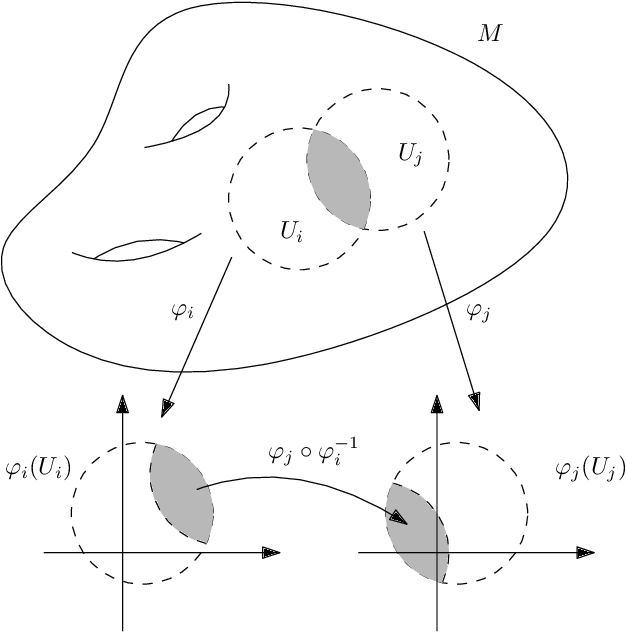
\includegraphics[width=0.3\linewidth]{Imagenes/atlas holomorfo}
			\caption{Representación de cartas holomorfa.}
			\label{fig:atlas-holomorfo}
		\end{figure}
		
	\end{enumerate}
	El par $(U_i,\varphi_i)$ es llamado \textbf{carta holomorfa} y la colección $\{(U_i,\varphi_i)\}$ de todas las cartas es llamado \textbf{atlas holomorfo}. Si existe un atlas holomorfo para $M$, también vamos a decir que \textbf{admite una estructura analítica}.
	Una \textbf{curva compleja} es una variedad compleja de dimensión $1$, y si además es conexa le llamamos \textbf{superficie de Riemann}. Por último, decimos que una variedad compleja de dimensión $2$ es una \textbf{superficie compleja}.
\end{definition}


\subsection{Ejemplos}
Ahora vamos a presentar varios ejemplos esenciales de variedades complejas.


\begin{example}[$ n $-espacio afín $\cc^n$]   
	Consideremos el espacio complejo $\cc^n$. Un atlas holomorfo para este espacio está dado por $\mathscr{A}=\{(\cc^n,\mathrm{id})\}$\footnote{Note que no es un atlas maximal.}, además de cumplir con todas las propiedades topológicas que necesitamos para ser una variedad compleja. Este será nuestro ejemplo base de variedad compleja no compacta. 
\end{example}

\begin{example}[Abierto de una variedad]
	Si $M$ es una variedad compleja con atlas holomorfo $\{(U_i,\varphi_i)\}$, entonces todo abierto no vacío $U\subset M$ es una variedad compleja con atlas holomorfo $\{(U\cap U_i,\varphi_i|_{U\cap U_i})\}$.
\end{example}

\begin{example}[Producto de variedades]
	Si $M_1,\dots, M_k$ son variedades complejas de dimensión $n_1,\dots,n_k$ respectivamente. Entonces el producto $M_1\times \cdots\times M_k$ es una variedad compleja de dimensión $n_1+\cdots+n_k$ cuyas cartas son de la forma $(U_1\times\cdots\times U_k,\varphi_1\times\cdots\times \varphi_k)$. Notemos que las cartas son compatibles pues
	\begin{equation*}
		(\psi_1\times\cdots\times \psi_k)\circ (\varphi_1\times\cdots\times \varphi_k)^{-1}=(\psi_1\circ\varphi_1^{-1})\times\cdots\times (\psi_k\circ \varphi_k^{-1})
	\end{equation*}
	es una aplicación holomorfa.
\end{example}

\begin{example}[Toro Complejo]
	Consideremos $V$ un $\cc$-espacio vectorial de dimensión $n$. Una \textbf{retícula} en $V$ es un subgrupo aditivo abeliano discreto $\Lambda\subset V$ generada por $2n$ vectores $v_1,\cdots,v_{2n}$ los cuales son linealmente independientes sobre $\rr$. El cociente $V/\Lambda$ es una variedad compleja de dimensión $n$ compacta y conexa (véase \parencite[Example 1.18]{leecomplex}). Además, se puede determinar un difeomorfismo entre $V/\Lambda$ y el producto de círculos $(S^1)^{2n}$.
	Un caso particularmente interesante es el cociente 
	\begin{equation*}
		T=\cc/\Lambda
	\end{equation*}
	donde $\Lambda=w_1\zz+w_2\zz$ y $w_1,w_2$ son linealmente independientes sobre $\rr$. Esta curva compleja es llamada \textbf{curva elíptica}.
	\begin{figure}[H]
		\centering
		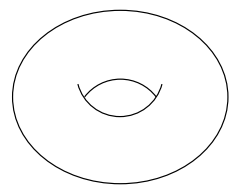
\includegraphics[width=0.25\linewidth]{Imagenes/toro}
		\caption{Modelo topológico de las curvas elípticas.}
		\label{fig:toro}
	\end{figure}
\end{example}

    \begin{example}[Variedades de Hopf]
	    	Consideremos $\lambda=(\lambda_1,\dots,\lambda_n)$ una $n$-tupla ordenada de números reales tal que $0<\lambda_i<1$, y definamos la acción $\cdot:\zz\times\cc^n\setminus\{0\}\to\cc^n\setminus\{0\}$ dada por
	    	\begin{equation*}
		    		k\cdot z=((\lambda_1)^kz_1,\dots,(\lambda_n)^kz_n).
		    	\end{equation*}
	    	Esta acción es holomorfa, libre y propia, por lo que el cociente bajo esta acción
	    	\begin{equation*}
		    		H=\frac{\cc^n\setminus\{0\}}{\zz}
		    	\end{equation*}
	    	es una variedad compleja conexa y compacta llamada \textbf{variedad de Hopf}. Más aún, esta variedad $H$ es difeomorfa a $S^{2n-1}\times S^1$. (veáse \parencite[Example 1.19]{leecomplex})
	    \end{example}

Ahora vamos a ver con detalle cómo los ceros de funciones holomorfas determinan variedades complejas. Lo anterior es fundamental para determinar la estructura analítica de las variedades algebraicas, pues los polinomios son funciones holomorfas.

\begin{example}[Hipersuperficie afín]
	Consideremos una función holomorfa $f:\cc^n\to \cc$ con $0\in\cc$ un valor regular. Sea
	\begin{equation*}
		X:=f^{-1}(0)=Z(f)\subset \cc^n
	\end{equation*}
	y $p\in X$. Escribiendo $f=f(z_1,\dots,z_n)$, el jacobiano de $f$ en $p$ está dado por
	\begin{equation*}
		J(f)(p)=\left(\frac{\partial f}{\partial z_1}(p),\dots, \frac{\partial f}{\partial z_n}(p)\right).
	\end{equation*}
	Como $0\in\cc$ es un valor regular, entonces $p$ es un punto regular. Así, el rango de la matriz $J(f)(p)$ (de tamaño $1\times n$) es $1$, es decir, al menos una derivada parcial no se anula en $p$. Sin pérdida de generalidad, podemos asumir que 
	\begin{equation*}
		\frac{\partial f}{\partial z_n}(p)\neq 0.
	\end{equation*}
	En particular, existe una vecindad $U\subset\cc^n$ de $p$ donde $\frac{\partial f}{\partial z_n}$ no se anula. Renombrando las coordenadas $w=(z_1,\dots,z_{n-1})$ y $z=z_n$, se puede escribir $f=f(w,z)$. Por el teorema de la función implícita \ref{funcionimplicita}, existe una vecindad $W\subset\cc^{n-1}$ de $w_0=(p_1,\dots,p_{n-1})$ y una función holomorfa $g:W\to\cc$ tal que $f(w,g(w))=0$ para todo $w\in W$ y  
	\begin{equation*}
		\{(w,z)\in W\times\cc:f(w,z)=0\}=\{(w,g(w)):w\in W\}.
	\end{equation*}
	Definamos ahora la función
	\begin{align*}
		\varphi:X\cap U&\longrightarrow W\subset\cc^{n-1}\\
		(w,z)&\longmapsto w.
	\end{align*}
	\begin{center}
		\begin{figure}[H]
			\centering
			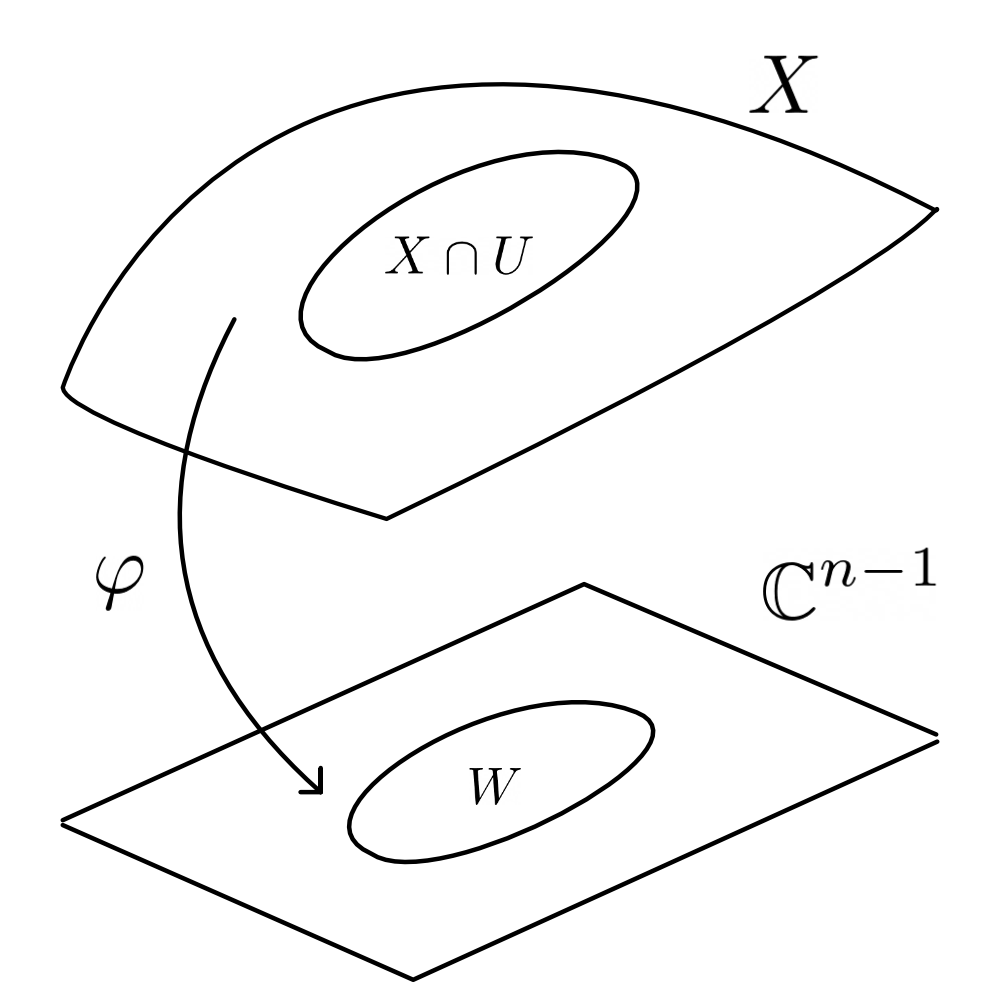
\includegraphics[width=0.3\linewidth]{Imagenes/hipersuperficie afin}
			\caption{Carta de la hipersuperficie afín.}
			\label{fig:hipersuperficie-afin}
		\end{figure}
	\end{center}
	Queremos ver que $\varphi$ es una carta para $p$. Probemos primero que es inyectiva y sobreyectiva.
	\begin{itemize}
		\item Sean $x,x'\in X\cap U$ tales que $\varphi(x)=\varphi(x')$. Si $x=(w,z)$ y $x'=(w',z')$, entonces $z=g(w)$ y $z'=g(w')$. Así,
		\begin{align*}
			\varphi(x)&=\varphi(x')\\
			w&=w'
		\end{align*}
		De esta forma, $z=z'$ y por tanto $x=x'$. Esto significa que $\varphi$ es inyectiva.
		\item Sea $w\in W$, entonces $(w,g(w))\in X\cap U$ y
		\begin{equation*}
			\varphi(w,g(w))=w.
		\end{equation*}
		Así, $\varphi$ es sobreyectiva.
	\end{itemize}
	Con esto, $\varphi$ es biyectiva y además la inversa de $\varphi$ está dada por
	\begin{align*}
		\varphi^{-1}:W\to X\cap U\\
		w\mapsto (w,g(w))
	\end{align*}
	
	Como $\varphi$ y $\varphi^{-1}$ son aplicaciones holomorfas, en particular son funciones continuas.
	Dado que todo punto de $X$ es regular, para cada $p\in X$ existe un abierto $U$ y una carta centrada en $p$. Ahora probemos que las funciones de transición son holomorfas.\\
	Sea $p\in X\cap U$ otro punto con carta $\psi:X\cap U'\to W'$, entonces
	\begin{equation*}
		\psi\circ\varphi^{-1}:\varphi((X\cap U)\cap(X\cap U'))\to\psi((X\cap U)\cap(X\cap U'))
	\end{equation*}
	es una función tal que 
	\begin{equation*}
		w\mapsto (w',g(w'))\mapsto w'
	\end{equation*}
	donde $w'$ es la proyección sobre las $n-1$ coordenadas elegidas por la carta $\psi$. Dado que ambas proyecciones son holomorfas, entonces la función de transición $\psi\circ\varphi^{-1}$ es holomorfa. Como $\varphi^{-1}$ está dada por $(w,g(w))$ y $\psi$ es una proyección de coordenadas, la composición $\psi\circ\varphi^{-1}$ es holomorfa.
	De esta manera, las cartas $(X\cap U,\varphi)$ dotan a $X$ de un atlas holomorfo.\\
	Más aún, $X$ como subespacio de $\cc^n$ es un espacio Hausdorff, segundo numerable y con estructura holomorfa. Por lo tanto, $X$ es una variedad compleja de dimensión $n-1$.
\end{example}

Generalizando este último ejemplo tenemos:
\begin{example}[Intersección compleja]\label{interseccioncompleja}
	Sean $k$ funciones holomorfas $f_1,f_2,\cdots,f_k:\cc^n\to \cc$, con $k\leq n$ y definamos la aplicación holomorfa asociada
	\begin{equation*}
		f=(f_1,\dots,f_k):\cc^n\to\cc^k.
	\end{equation*}   
	Supongamos que $0\in\cc^k$ es un valor regular de $f$. Entonces el conjunto
	\begin{equation*}
		X:=f^{-1}(0)=Z(f_1)\cap\cdots\cap Z(f_k)=Z(f_1,\dots,f_k)
	\end{equation*}
	es una variedad compleja de dimensión $n-k$.\\
	La demostración sigue la misma estrategia para el caso $k=1$ con ciertas observaciones:
	\begin{itemize}
		\item Para cada punto $p\in X$, el rango de la matriz jacobiana $J(f)(p)$ es $k$. Por una renumeración de las variables, podemos suponer que la submatriz cuadrada de las últimas $k$ variables tiene determinante no cero.
		\item Por el teorema de la función implícita, tenemos una vecindad $W\subset\cc^{n-k}$ de las primeras $n-k$ entradas de $p$, una vecindad $Z\subset\cc^k$ de las últimas $k$ entradas de $p$ y una aplicación holomorfa
		\begin{equation*}
			g:W\to Z
		\end{equation*}
		\item Las cartas $\varphi:X\cap U\to W\subset\cc^{n-k}$ se construyen de la misma manera y la transición sigue siendo holomorfa como antes, por componerse de proyecciones y las funciones holomorfas $g$.
	\end{itemize}
	
\end{example}

\begin{example}[Espacio proyectivo]
	El \textbf{n-espacio proyectivo} es el conjunto $\pp^n=\cc^{n+1}\setminus\{0\}/\sim$ donde $z,w\in\cc^{n+1}\setminus\{0\}$ están relacionados si, y solo si, existe $\lambda\in\cc\setminus\{0\}$ tal que  $z=\lambda w$.
	
	Dotamos a $\pp^n$ con la topología cociente dada por la proyección canónica
	\begin{equation*}
		q:\cc^{n+1}\setminus \{0\} \longrightarrow \pp^n
	\end{equation*}
	Consideremos la cubierta estándar afín de $\pp^n$ dada por los $n+1$ abiertos
	\begin{equation*}
		U_i=\{[x_0:\cdots:x_n]:x_i\neq 0\}\subset \pp^n
	\end{equation*}
	Así, tenemos las funciones $\varphi_i:U_i\to\cc^n$ dadas por
	\begin{align*}
		[x_0:x_1:\dots:x_n]\mapsto & \left( \frac{x_0}{x_i},\frac{x_1}{x_i},\dots, \frac{x_{i-1}}{x_i},\frac{x_{i+1}}{x_i},\dots,\frac{x_n}{x_i}\right)
	\end{align*} 
	Estas funciones son continuas por la propiedad característica de la topología cociente y su inversa está dada por
	\begin{equation*}
		\varphi_{i}^{-1}(z_1,\dots,z_n)=[z_1:\dots:z_{i-1}:1:z_{i+1}:\dots:z_n]
	\end{equation*}
	Así, las funciones $\varphi_i$ son homeomorfismos llamados \textbf{cartas afines}.
	Además, las funciones de transición $\varphi_{ij}=\varphi_i\circ\varphi_j^{-1}:\varphi_j(U_i\cap U_j)\to\varphi_i(U_i\cap U_j)$ están dadas por
	\begin{equation*}
		\varphi_{ij}(w_1,\dots,w_n)=\left(\frac{w_1}{w_i},\dots \frac{w_{i-1}}{w_i},\frac{w_{i+1}}{w_i},\dots,\frac{w_{j-1}}{w_i},\frac{1}{w_i},\frac{w_{j+1}}{w_i},\dots,\frac{w_n}{w_i} \right)
	\end{equation*}
	Notemos que $\varphi_i(U_i \cap U_j)=\cc^n\setminus Z(w_j)$. Con esto, las funciones $\varphi_{ij}$ son aplicaciones holomorfas.\\
	Las propiedades topológicas de Hausdorff y segundo numerable son análogas al caso de $\pp^1$ (véase \parencite[Cap. 1, Sec. 1, Ejem. 1.3]{zaldrimann}).\\
	Si consideramos la esfera $S^{2n+1}$ unitaria de $\cc^{n+1}$, entonces tenemos la siguiente composición de funciones continuas\footnote{A la tríada $(S^{2n+1},q,\pp^n)$ se le llama \textbf{fibrado de Hopf}.}
	\[\begin{tikzcd}
		{S^{2n+1}} && {\cc^{n+1}\setminus\{0\}} \\
		\\
		&& {\mathbb{P}^n}
		\arrow[hook, from=1-1, to=1-3]
		\arrow["\rho"', dashed, from=1-1, to=3-3]
		\arrow["p", two heads, from=1-3, to=3-3]
	\end{tikzcd}\]
	Como $\pp^n$ es la imagen continua de $S^{2n+1}$ bajo $\rho$ y la esfera es conexa y compacta, entonces podemos concluir que el espacio proyectivo $\pp^n$ es conexo y compacto.
	Por lo tanto, $\pp^n$ es una variedad compleja conexa y compacta.
\end{example}
\begin{figure}[H]
	\centering
	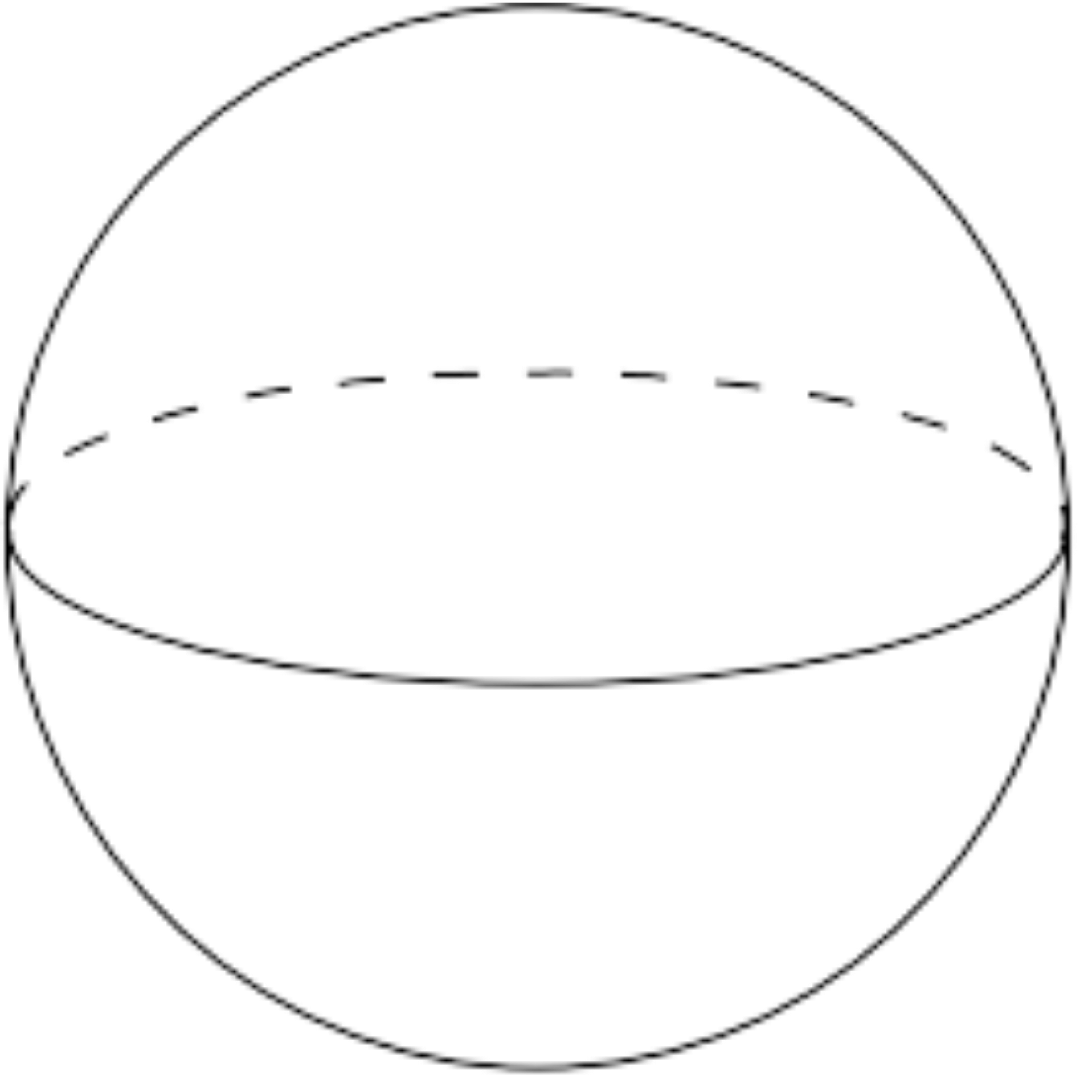
\includegraphics[width=0.2\linewidth]{Imagenes/Esfera}
	\caption{Recta proyectica $\pp^1$}
	\label{fig:esfera}
\end{figure}

En este trabajo nos enfocaremos principalmente en las variedades compactas conexas, pues muchos resultados importantes se sustentan bajo estas hipótesis y son esenciales para el tema de algebrización. Veremos con más detalle esto último en el segundo capítulo.

\subsection{La esfera de Riemann}

Aquí desarrollaremos tres ejemplos de superficies de Riemann que pueden verse distintos, pero que en esencia serán la misma superficie. Especificamente hablamos de la esfera unitaria en $\rr^3$, el plano extendido $\overline{\cc}:=\cc\cup \{\infty\}$ y la recta proyectiva compleja $\pp^1$. Es conocido que topológicamente estos espacios son homeomorfos y por consecuencia superficies de género $0$ (falta cita). Sin embargo, veremos que sus estructuras holomorfas serán también compatibles. Siendo exactos, estos tres espacios serán biholomorfos (falta cita).

\begin{example}[Esfera de Riemann]
	Considere la esfera unitaria en $\rr^3$ dada por
	\begin{equation*}
		S^2=\{(x_1,x_2,x_3)\in\rr^3:x_1^2+x_2^2+x_3^2=1\}
	\end{equation*}
	Podemos dotar a $S^2$ con la topología del subespacio y de esta manera $S^2$ es conexo, Hausdorff y segundo numerable.
	\begin{figure}[H]
		\centering
		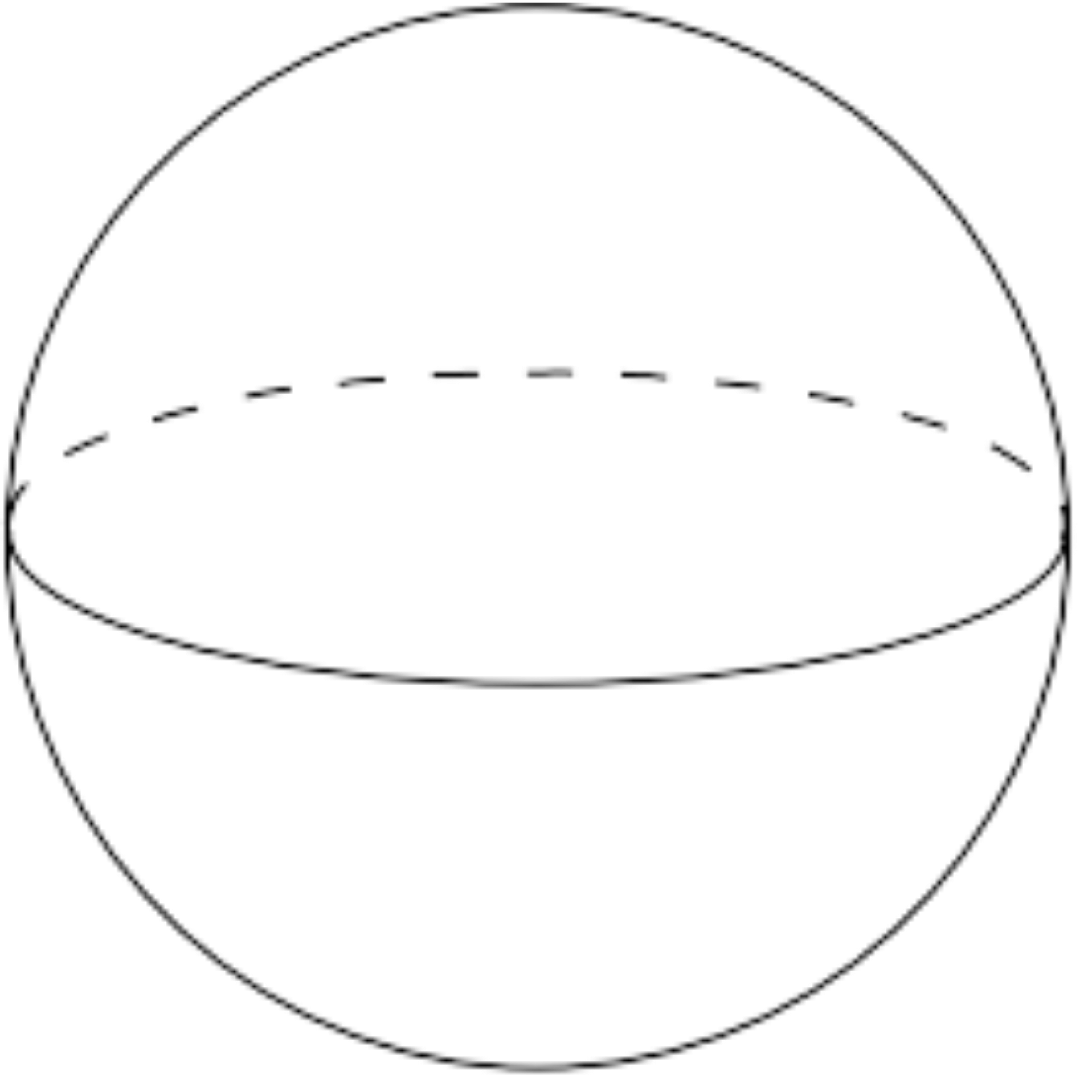
\includegraphics[width=0.25\linewidth]{Imagenes/Esfera.png}
		\caption{Esfera de Riemann \cite[Fig. 10.1, p. 170]{Sambarino}}
	\end{figure}
	Definamos la cubierta
	\begin{equation*}
		U_0=S^2\setminus(0,0,1),\qquad U_1=S^2\setminus(0,0,-1)
	\end{equation*}
	y las funciones 
	\begin{equation*}
		\varphi_0:U_0\to\cc,\qquad \varphi_1:U_1\to\cc
	\end{equation*}
	dadas por
	\begin{equation*}
		\varphi_0(x_1,x_2,x_3)=\frac{x_1}{1-x_3}+i\frac{x_2}{1-x_3},\qquad \varphi_1(x_1,x_2,x_3)=\frac{x_1}{1+x_3}-i\frac{x_2}{1+x_3}
	\end{equation*}
	Note que las funciones son continuas por criterio por componentes.\\
	Además, se puede determinar que $\varphi^{-1}_0:\cc\to U_0$ y $\varphi^{-1}_1:\cc\to U_1$ dadas por
	\begin{equation*}
		\varphi^{-1}_0(z)=\left( \frac{2\mathrm{Re}(z)}{1+|z|^2},\frac{2\mathrm{Im}(z)}{1+|z|^2},\frac{1-|z|^2}{1+|z|^2} \right)\qquad \varphi^{-1}_1(z)=\left( \frac{2\mathrm{Re}(z)}{1+|z|^2},-\frac{2\mathrm{Im}(z)}{1+|z|^2},\frac{1-|z|^2}{1+|z|^2} \right)
	\end{equation*}
	Luego, $U_0\cap U_1=S^2\setminus\{(0,0,1),(0,0,-1)\}$. Si $z\in \cc\setminus\{0\}$, entonces
	\begin{equation*}
		\left( \frac{2\mathrm{Re}(z)}{1+|z|^2},\frac{2\mathrm{Im}(z)}{1+|z|^2},\frac{1-|z|^2}{1+|z|^2} \right)\in U_0\cap U_1
	\end{equation*}
	y 
	\begin{equation*}
		\varphi_0\left( \frac{2\mathrm{Re}(z)}{1+|z|^2},\frac{2\mathrm{Im}(z)}{1+|z|^2},\frac{1-|z|^2}{1+|z|^2} \right)=z
	\end{equation*}
	De esta manera, $\varphi_0(U_0\cap U_1)=\cc\setminus\{0\}$. Análogamente, $\varphi_1(U_0\cap U_1)=\cc\setminus\{0\}$.\\
	Así, $\varphi_0(U_0\cap U_1)=\varphi_1(U_0\cap U_1)$ es un abierto en $\cc$ (por ser complemento de un conjunto unipuntual).\\
	Considerando la función de transición
	\begin{equation*}
		\varphi_{01}=\varphi_0\circ \varphi_1^{-1}:\varphi_1(U_0\cap U_1)\to\varphi_0(U_0\cap U_1)
	\end{equation*}
	se tiene que
	\begin{align*}
		\varphi_0\circ \varphi_1^{-1}(z)&=\varphi_0\left( \frac{2\mathrm{Re}(z)}{1+|z|^2},-\frac{2\mathrm{Im}(z)}{1+|z|^2},\frac{1-|z|^2}{1+|z|^2} \right)\\
		&=\frac{\frac{2\mathrm{Re}(z)}{1+|z|^2}}{1-\frac{1-|z|^2}{1+|z|^2}}+i\frac{-\frac{2\mathrm{Im}(z)}{1+|z|^2}}{1-\frac{1-|z|^2}{1+|z|^2}}\\
		&=\frac{2\mathrm{Re}(z)}{2|z|^2}-i\frac{2\mathrm{Im}(z)}{2|z|^2}\\
		&=\frac{\mathrm{Re}(z)-\mathrm{Im}(z)i}{|z|^2}\\
		&=\frac{\mathrm{Re}(z)-\mathrm{Im}(z)i}{(\mathrm{Re}(z)-\mathrm{Im}(z)i)(\mathrm{Re}(z)-\mathrm{Im}(z)i)}\\
		&=\frac{1}{z}
	\end{align*}
	la cual está bien definida ya que $\varphi_1(U_0\cap U_1)=\cc\setminus\{0\}$. Además, es holomorfa en todo su dominio.\textbf{Aquí una imagen}\\
	Esto implica que $\mathscr{A}=\{(U_0,\varphi_0),(U_1,\varphi_1)\}$ es un atlas holomorfo para $S^2$.\\
	De esta manera, $S^2$ es una superficie de Riemann. Más aún, por el teorema de Heine-Borel, $S^2$ es compacto. Por lo tanto, $S^2$ es una superficie de Riemann compacta.
\end{example}

\begin{example}[Plano Complejo Extendido]
	El plano complejo extendido $\overline{\cc}=\cc\cup\{\infty\}$ es un espacio topológico Hausdorff compacto \parencite{schlag}.\\
	Consideremos la cubierta $\{U_0,U_1\}$
	\begin{equation}
		U_0=\overline{\cc}\setminus\{\infty\},\qquad U_1=\overline{\cc}\setminus\{0\}
	\end{equation}
	con las funciones $\varphi_0:U_0\to\cc$ y $\varphi_1:U_1\to\cc$ dadas por
	\begin{align*}
		\varphi_0(z)&=z\\
		\varphi_1(z)&=\begin{cases}
			0,&\enspace z=\infty\\
			1/z,&\enspace z\neq \infty
		\end{cases}
	\end{align*}
	La funcion de transición son de la forma
	\begin{align*}
		\varphi_0\circ \varphi_1^{-1}:&\cc\setminus\{0\}\to \cc\setminus\{0\}\\
		&z\mapsto \frac{1}{z}
	\end{align*}
	Notemos que es la misma que la esfera de Riemann
\end{example}

\begin{example}[Recta Proyectiva Compleja]\label{recta proyectiva}
	Considere sobre $\cc^2\setminus\{(0,0)\}$ la siguiente relación de equivalencia 
	\begin{equation*}
		(z_1,w_1)\sim (z_2,w_2)\qquad\text{ si y solo si}\qquad\text{existe }\lambda\in\cc\setminus\{0\}\text{ tal que } (z_1,w_1)=\lambda(z_2,w_2)
	\end{equation*}
	Notemos que
	\begin{itemize}
		\item $(z_1,w_1)\sim (z_1,w_1)$ con $\lambda=1$.
		\item Si $(z_1,w_1)\sim (z_2,w_2)$, entonces existe $\lambda\in\cc\setminus\{0\}$ tal que 
		\begin{align*}
			(z_1,w_1)&=\lambda(z_2,w_2)\\
			\frac{1}{\lambda} (z_1,w_1)&=(z_2,w_2)
		\end{align*}
		Entonces, $(z_2,w_2)\sim (z_1,w_1)$.
		\item Si $(z_1,w_1)\sim (z_2,w_2)$ y $(z_2,w_2)\sim (z_3,w_3)$, entonces  
		\begin{align*}
			(z_1,w_1)&=\lambda_1(z_2,w_2),\qquad\lambda_1\in\cc\setminus\{0\}\\
			(z_2,w_2)&=\lambda_2(z_3,w_3),\qquad\lambda_2\in\cc\setminus\{0\}
		\end{align*}
		Así,
		\begin{equation*}
			(z_1,w_1)=\lambda_1\lambda_2(z_3,w_3)
		\end{equation*}
		Con esto, $\sim$ es una relación de equivalencia.\\ 
		
	\end{itemize}
	Definamos el conjunto 
	\begin{equation*}
		\mathbb{P}^1=\cc^2\setminus\{(0,0)\}/\sim
	\end{equation*}
	Denotamos por $[(z,w)]:=[z:w]$ a los elementos de $\pp^1$ y se llamados \textcolor{blue}{coordenadas homogéneas}.\\
	Sean 
	\begin{align*}
		U_0:=\{[z:w]:z\neq 0\} \\
		U_1=\{[z:w]:w\neq 0\} 
	\end{align*}
	Notemos que $\pp^1=U_0\cup U_1$. 
	Consideremos las funciones $\varphi_0:U_0\to\cc$ y $\varphi_1:U_1\to\cc$ dadas por
	\begin{equation*}
		\varphi_0([z:w])=\frac{w}{z},\qquad \varphi_1([z:w])=\frac{z}{w}
	\end{equation*}
	Notemos que si $z\in\cc$, entonces
	\begin{align*}
		\varphi_0^{-1}(z)= \varphi_0^{-1}\left(\frac{z}{1}\right)=[1:z]\in U_0\\
		\varphi_1^{-1}(z)= \varphi_1^{-1}\left(\frac{z}{1}\right)=[z:1]\in U_1\\
	\end{align*}
	Más aún, si $w\in\cc\setminus\{0\}$ tenemos que $[1:w],[w:1]\in U_0\cap U_1$ y $\varphi_0[1:w]=\varphi_1[w:1]=w$. De esta manera, $\varphi_0(U_0\cap U_1)=\varphi_1(U_0\cap U_1)=\cc\setminus\{0\}$, el cual es abierto en $\cc$.\\
	Más aún, si $z\in\cc\setminus\{0\}$, entonces
	\begin{align*}
		\varphi_{01}=(\varphi_0\circ\varphi_1^{-1})(z)=\varphi_0(\varphi_1^{-1}(z))=\varphi_0([z:1])=\frac{1}{z}\\
		\varphi_{10}=(\varphi_1\circ\varphi_0^{-1})(z)=\varphi_1(\varphi_0^{-1}(z))=\varphi_1([1:z])=\frac{1}{z}
	\end{align*}
	Así, $\varphi_{01}$ y $\varphi_{10}$ son holomorfas en $\cc\setminus\{0\}$ (notemos que son las mismas que en la esfera). Así, $\{(U_0,\varphi_0),(U_1,\varphi_1)\}$ es un atlas holomorfo para $\pp^1$.\\
	Ahora, probemos las propiedades topológicas de $\pp^1$.\\
	Por construcción, las cartas $\varphi_i$ son homeomorfismos. Como $\cc$ es conexo, entonces $U_0$ y $U_1$ son conexos (por ser imagen de un conexo bajo la función continua $\varphi_i^{-1})$. Además, como $U_0\cap U_1\neq\emptyset$ entonces $\pp^1=U_0\cup U_1$ es conexo. Dado que $\varphi_i:U_i\to\cc$ son homeomorfismos y $\cc$ es Hausdorff, entonces $U_i$ son hausdorff.\\
	Así, si $[z_0:w_0]$ y $[z_1:w_1]$ pertenecen al mismo tiempo a $U_0$ o $U_1$, entonces podemos separarlos por abiertos disjuntos.
	De esta manera, tomemos puntos $[z_0:w_0],[z_1:w_1]\in\pp^1$ tales que $[z_0:w_0]\in U_0\setminus U_1$ y $[z_1:w_1]\in U_1\setminus U_0$.\\
	Notemos que $[z_0:w_0]\in U_0\setminus U_1$ implica que $z\neq 0$ y $w_0=0$. Entonces\\ $[z_0:w_0]=[z_0:0]=[1:0]$.
	Análogamente, $[z_1:w_1]=[0:1]$. Luego
	\begin{equation*}
		\varphi_0[1:0]=0\in B_1(0),\qquad \varphi_1[0:1]=0\in B_1(0)
	\end{equation*}
	donde $B_1(0)\subset \cc$ es la bola abierta de radio 1 centrada en $0$. De este modo, $[1:0]\in \varphi
	_0^{-1}(B_1(0))$ y $[0:1]\in \varphi
	_1^{-1}(B_1(0))$.
	\begin{center}
		\begin{tikzcd}
			{[1:0]\in U_0\setminus U_1} && {[0:1]\in U_1\setminus U_0} \\
			\\
			& {B_1(0)}
			\arrow["{\varphi_0}"', from=1-1, to=3-2]
			\arrow["{\varphi_1}", from=1-3, to=3-2]
		\end{tikzcd}
	\end{center}
	Ahora, supongamos que existe $[z:w]\in\varphi_0^{-1}(B_1(0))\cap \varphi_1^{-1}(B_1(0))$. Entonces
	\begin{equation*}
		\varphi_0[z:w]=\frac{w}{z}\in B_1(0),\qquad \varphi_1[z:w]=\frac{z}{w}\in B_1(0) 
	\end{equation*}
	Esto implica que $\frac{|w|}{|z|}<1$ y $\frac{|z|}{|w|}<1$. Entonces
	\begin{equation*}
		|w|<|z|,\qquad\text{y}\qquad |z|<|w|
	\end{equation*}
	lo cual es imposible.\\
	Así, $\varphi_0^{-1}(B_1(0))\cap\varphi_1^{-1}(B_1(0))=\emptyset$. De esta manera, $\pp^1$ es Hausdorff.\\
	Más aún, sea $[z:w]\in\pp^1$ y supongamos que $z\neq 0$. Si $\varphi_0[z:w]=\frac{w}{z}\in \overline{B_1(0)}$, entonces $[z:w]\in\varphi_0^{-1}(\overline{B_1(0)})$.\\
	Pero si $\varphi_0[z:w]=\frac{w}{z}\not\in\overline {B_1(0)}$, entonces $w\neq 0$ y 
	\begin{align*}
		\frac{|w|}{|z|}<1\\
		1<\frac{|z|}{|w|}
	\end{align*}
	Esto es, $\varphi_1[z:w]\in B_1(0)\subset \overline{B_1(0)}$.\\
	Así, $\pp^1=\varphi_0^{-1}(\overline{B_1(0)})\cup \varphi_1^{-1}(\overline{B_1(0)})$. Como $\overline{B_1(0)}$ es compacto, entonces $\varphi_0^{-1}(\overline{B_1(0)})$ y $\varphi_1^{-1}(\overline{B_1(0)})$ son compactos. Por lo tanto, $\pp^1$ es compacto.\\
\end{example}
$\pp^1$ es una superficie de Riemann compacta llamada \textcolor{blue}{recta proyectiva compleja}.



\section{Aplicaciones Holomorfas}

Pese a que las funciones holomorfas son suaves, estas mismas tienen una rigidez mucho mayor que las funciones suaves en la geometría diferencial real. Como en el análisis complejo, esta diferencia tiene consecuencias profundas en el estudio de estos objetos, y en consecuencia también cambia la situación geométrica con respecto a la real. Por ejemplo, en la geometría diferencial real la orientabilidad es una condición adicional y fundamental para teoremas importantes, en geometría compleja se demuestra que toda variedad compleja es orientable. Por otra parte, la estructura del anillo de funciones holomorfas globales sobre una variedad compleja compacta es altamente restrictiva (véase teorema \ref{holomorfasglobal}).

Vamos a establecer las formalidades sobre morfismos entre variedades complejas en fin de comprender la riqueza analítica de las mismas.

\begin{definition}[Aplicación holomorfa]
	Sean $M$ y $N$ dos variedades complejas. Una \textbf{aplicación holomorfa} entre $M$ y $N$ es una función continua $f:M\to N$ tal que para cada $p\in M$, para cada carta $(U,\varphi)$ alrededor de $p\in M$ y $(V,\psi)$ alrededor de $f(p)\in N$, la función
	\begin{equation*}
		\psi\circ f\circ \varphi^{-1}:\varphi(U\cap f^{-1}(V))\longrightarrow\psi(V)
	\end{equation*}
	es una aplicación holomorfa en $\varphi(p)$.
	\begin{center}
		\begin{tikzcd}
			{p\in U} && {f(p)\in V} \\
			\\
			{\varphi(U\cap f^{-1}(V))} && {\psi(V)}
			\arrow["f", from=1-1, to=1-3]
			\arrow["\varphi"', from=1-1, to=3-1]
			\arrow["\psi", from=1-3, to=3-3]
			\arrow["{\psi\circ f\circ \varphi^{-1}}"', from=3-1, to=3-3]
		\end{tikzcd}
	\end{center}
\end{definition}

\begin{definition}
	Una aplicación holomorfa $f:M\to N$ entre variedades complejas se llama \textbf{biholomorfismo} si es biyectiva y su inversa también es una aplicación holomorfa. Dos variedades complejas se dicen \textbf{biholomorfas} si existe un biholomorfismo entre ellas.
\end{definition}

\begin{remark}
	Dada una función continua $f:M\to N$, la propiedad de ser holomorfa es independiente de la elección de las cartas holomorfas de la estructura holomorfa de $M$ y $N$. Así, la verificación de la propiedad puede realizarse para cualquier atlas de $M$ y $N$.
\end{remark}

\begin{lemma}$ $
	\begin{enumerate}
		\item La restricción de una aplicación holomorfa a un subconjunto abierto es holomorfa.
		\item Toda aplicación constante entre variedades complejas es una aplicación holomorfa.
		\item La aplicación identidad sobre cualquier variedad compleja es una aplicación holomorfa.
		\item Toda carta holomorfa es un biholomorfismo sobre su imagen.
		\item La composición de aplicaciones holomorfas es una aplicación holomorfa.
	\end{enumerate}
\end{lemma}

Tenemos muchos resultados enigmáticos de las funciones holomorfas y resulta interesante ver sus consecuencias en las aplicaciones holomorfas entre variedades complejas. Uno de los más importantes, y una primera distinción frente a las variedades reales, es el \textit{teorema de la identidad}.

\begin{theorem}[Teorema de la identidad]\label{teoidentidad}
	Sean $M$ y $N$ dos variedades complejas, con $M$ conexa y $f,g:M\to N$ dos aplicaciones holomorfas que coinciden en un subconjunto abierto no vacío de $M$. Entonces $f=g$. 
\end{theorem}
\begin{proof}
	Comencemos definiendo el conjunto
	\begin{equation*}
		A=\{p\in M:f\text{ y }g\text{ coinciden en una vecindad de }p\ \}.
	\end{equation*}
	Queremos demostrar que este conjunto es abierto y cerrado. Dado que $M$ es conexo, tendríamos que $A=M$.
	\begin{itemize}
		\item Sea $p\in A$, entonces existen cartas $(U,z)$ alrededor de $p$ y $(V,w)$ en $N$ tales que
		\begin{equation*}
			f(U),g(U)\subset V.
		\end{equation*}
		Como $f$ y $g$ son aplicaciones holomorfas, entonces las funciones $w\circ f\circ z^{-1}$ y $w\circ g\circ z^{-1}$ son holomorfas en $z(U)$. Además, como $p\in A$ entonces existe una vecindad $W\subset M$ de $p$ donde $f$ y $g$ coinciden. Así,
		\begin{equation*}
			(w\circ f\circ z^{-1})\left.\right|_{z(U\cap W)}=(w\circ g\circ z^{-1})\left.\right|_{z(U\cap W)}.
		\end{equation*} 
		Por el teorema de la identidad \ref{identidad}, las funciones coinciden en todo $z(U)$.
		Por lo que, $f=g$ en todo $U$ y $U\subset A$.\\
		De esta forma, $p$ es un punto interior de $A$ y concluimos que $A$ es un conjunto abierto.
		
		\item Supongamos que $b\in \partial A$. Queremos probar que $b\in A$ para concluir que $A$ es cerrado.
		Como $b$ pertenece a la frontera de $A$ y $f$ y $g$ coinciden en $A$, por continuidad tenemos que $f(b)=g(b)$. Tomemos cartas $(U,z)$ de $M$ alrededor de $b$ y $(V,w)$ de $N$ alrededor de $f(b)=g(b)\in N$, con $U$ conexo. Definamos
		\begin{align*}
			F&=w\circ f\circ z^{-1}:z(U)\to w(V),\\
			G&=w\circ g\circ z^{-1}:z(U)\to w(V),
		\end{align*}
		las cuales son holomorfas por hipótesis.\\
		Ahora, como $b\in\partial A$, cualquier vecindad de $b$ debe intersectar $A$. En particular, $U\cap A\neq\emptyset$, ya que si esto no ocurriera, entonces $U\subseteq M\setminus A$ y por lo tanto $b$ estaría en el interior de $M\setminus A$, contradiciendo que $b\in\partial A$.\\
		De esta manera, podemos tomar $p\in U\cap A$. Por definición de $A$, $f=g$ en una vecindad $W\subset U$ de $p$ tal que
		$$
		f|_W = g|_W.
		$$
		Al pasar a las coordenadas locales,
		esto significa que $F=G$ en el abierto no vacío $z(W)\subseteq z(U)$. Como $F$ y $G$ son holomorfas y coinciden en un subconjunto abierto de $z(U)$, por el teorema de identidad \ref{identidad}, tenemos que
		
		$$
		F = G \quad \text{en todo } z(U).
		$$
		
		Con lo cual $f=g$ en todo $U$, y en particular en una vecindad de $b$. Por lo tanto, $b\in A$.
	\end{itemize}
\end{proof}


\begin{corollary}
	Sea $f:M\to N$ una aplicación holomorfa propia y biyectiva entre variedades complejas de la misma dimensión, entonces $f$ es un biholomorfismo.
\end{corollary}
\begin{proof}
	Primero probemos que $f$ es un homeomorfismo.
	
	Dado que $f$ es una aplicación continua propia entre espacios Hausdorff y localmente compactos, entonces $f$ es cerrada. Además, como $f$ es biyectiva, su inversa $f^{-1}:N\to M$ cumple que la preimagen de cerrados es cerrado. Así, $f^{-1}$ es continua. Por lo que $f$ es un homeomorfismo. 
	
	Tomemos cartas $(U,\varphi)$ de $M$ y $(V,\psi)$ de $N$ con $f(U)\subset V$. Entonces la aplicación
	\begin{equation*}
		g:=\psi\circ f\circ \varphi^{-1}:\varphi(U)\subset\cc^n\longrightarrow \psi(V)\subset\cc^n
	\end{equation*}
	es holomorfa e inyectiva (pues $f$ lo es). Por la proposición \ref{biholomorfismojac}, $g$ es un biholomorfismo. Es decir, la aplicación
	\begin{equation*}
		g^{-1}=\varphi\circ f^{-1}\circ \psi^{-1}
	\end{equation*}
	es holomorfa. Solo basta probar que $f^{-1}$ es holomorfa para concluir que $f$ es biholomorfa. En efecto, si tomamos las cartas $(U',\varphi')$ de $M$ y $(V',\psi')$ de $N$ tales que intersectan a las cartas $(U,\varphi)$ y $(V,\psi)$, entonces
	\begin{align*}
		\varphi'\circ f^{-1}\circ \psi^{-1}&=\varphi'\circ (\varphi^{-1}\circ g^{-1}\circ \psi)\circ (\psi')^{-1}\\
		&=(\varphi'\circ \varphi^{-1})\circ g^{-1}\circ (\psi\circ (\psi')^{-1}).
	\end{align*}
	Como $(\varphi'\circ \varphi^{-1})$, $g^{-1}$ y $(\psi\circ (\psi')^{-1})$ son holomorfas, entonces $\varphi'\circ f^{-1}\circ \psi^{-1}$ es holomorfa. Por definición, $f^{-1}$ es holomorfa.
	\begin{center}
		\begin{tikzcd}
			{\psi(V')} && N && M && {\varphi'(U')} \\
			\\
			&& {\psi(V)} && {\varphi(U)}
			\arrow[from=1-1, to=3-3]
			\arrow["{\psi'}"', from=1-3, to=1-1]
			\arrow["{f^{-1}}", from=1-3, to=1-5]
			\arrow["\psi"', from=1-3, to=3-3]
			\arrow["{\varphi'}", from=1-5, to=1-7]
			\arrow["\varphi"', from=1-5, to=3-5]
			\arrow["{g^{-1}}"', from=3-3, to=3-5]
			\arrow[from=3-5, to=1-7]
		\end{tikzcd}
	\end{center}
\end{proof}

\subsection{Funciones holomorfas}
En geometría, es un principio bien establecido que el estudio de un objeto geométrico se apoya en el análisis de las funciones definidas sobre el objeto. Para nuestros objetivos, las funciones holomorfas desempeñan un papel importantísimo para las propiedades algebraicas de las variedades complejas.

\begin{definition}[Función holomorfa]
	Sea $M$ variedad compleja. Una \textbf{función holomorfa} en $M$ es una aplicación holomorfa $f:X\to\cc$, ya que $\cc$ es una variedad compleja. Específicamente, $f:M\to \cc$ es una función holomorfa si para todo punto $p\in M$ y cualquier carta $(U,\varphi)$ alrededor de $p\in M$, la función
	\begin{equation*}
		f\circ \varphi^{-1}:\varphi(U)\subset\cc^n\to\cc
	\end{equation*}
	es holomorfa en el sentido usual de funciones de varias variables complejas.
\end{definition}

\begin{center}
	\begin{tikzpicture}[>=stealth, scale=0.7]
		
		% 1. Variedad M (Manifold)
		% Dibujamos la forma de la variedad usando una curva suave cerrada
		\draw plot[smooth cycle, tension=0.7] coordinates {
			(-3, 2.5) 
			(-1.5, 4.2) 
			(2.5, 4) 
			(4.2, 2.5) 
			(3.5, 1.2) 
			(1, 0.8) 
			(-2, 0.5)
		};
		% Etiqueta M
		\node at (-3.5, 4) {\Large $M$};
		
		% 2. Subconjunto U
		\draw (-1, 2.2) ellipse (1.6 and 1.1);
		\node at (-1, 2.2) {\large $U$};
		
		% 3. Agujero / Género (Para denotar que es una superficie)
		\draw (1.5, 2.5) to[bend right=45] (2.9, 2.5);
		\draw (1.65, 2.35) to[bend left=45] (2.75, 2.35);
		
		% 4. Plano Complejo C (Arriba a la derecha)
		% Ejes
		\draw[->] (5, 2) -- (9, 2);
		\draw[->] (7, 0.5) -- (7, 3.5);
		% Etiqueta C
		\node at (8.5, 3.6) {\Large $\mathbb{C}$};
		
		% 5. Espacio de la carta phi(U) (Abajo a la izquierda)
		% Ejes (desfasados respecto al centro del círculo, como en la imagen)
		\draw[->] (-4.5, -3) -- (-1, -3);
		\draw[->] (-3.6, -4.5) -- (-3.6, -0.5);
		% Círculo
		\draw (-2.8, -2.5) circle (1.2);
		% Etiqueta phi(U)
		\node at (-2.7, -2.2) {$\varphi(U)$};
		
		% 6. Flechas y Mapeos
		% Flecha f
		\draw[->] (4.4, 3.3) to[bend left=12] node[above] {$f$} (6.2, 3.3);
		
		% Flecha phi
		\draw[->] (-1.8, 0.8) to[bend right=15] node[left, xshift=-2pt] {$\varphi$} (-2.6, -0.3);
		
		% Flecha f o phi^{-1}
		\draw[->] (-1.3, -1.6) to[bend left=15] node[below right, yshift=-2pt] {$f \circ \varphi^{-1}$} (5, 0.5);
		
	\end{tikzpicture}
	\captionof{figure}{Definición de función holomorfa} 
	\label{fig:funcion-holomorfa}
\end{center}


\begin{lemma}
	Sea $M$ una variedad compleja y $f:M\to\cc$ una función. Entonces $f$ es holomorfa en $p\in M$ si, y solo si, existe una carta $(U,\varphi)$ alrededor de $p$ tal que la función $f\circ \varphi^{-1}$ es holomorfa en $\varphi(p)$.
\end{lemma}
\begin{proof}
	Supongamos que existe una carta $(U,\varphi)$ alrededor de $p$ tal que la función $f\circ \varphi^{-1}$ es holomorfa en $\varphi(p)$. Sea $(V,\psi)$ una carta alrededor de $p$ tal que $U\cap V\neq \emptyset$. Así
	\begin{equation*}
		f\circ \psi^{-1}=(f\circ\varphi^{-1})\circ(\varphi\circ\psi^{-1})
	\end{equation*}
	Como cada paréntesis corresponde a una función holomorfa, entonces $f\circ \psi^{-1}$ es una función holomorfa.\\
	\begin{center}
		\begin{tikzcd}
			{\psi(V)\subset\mathbb{C}^n} && M && {\mathbb{C}} \\
			\\
			&& {\varphi(U)\subset\mathbb{C}^n}
			\arrow["{\varphi\circ\psi^{-1}}"', from=1-1, to=3-3]
			\arrow["\psi"', from=1-3, to=1-1]
			\arrow["f", from=1-3, to=1-5]
			\arrow["\varphi"', from=1-3, to=3-3]
			\arrow["{f\circ\varphi^{-1}}"', from=3-3, to=1-5]
		\end{tikzcd}
	\end{center}
	
	La otra implicación es clara por la definición.
\end{proof}

Este lema muestra que para comprobar que una función es holomorfa en un punto, es suficiente con hacerlo en una sola carta alrededor del punto. Se puede también hacer una demostración similar para aplicaciones en general pero requiere un diagrama bastante más grande. 

Resulta ser de bastante interés construir objetos algebraicos a partir de objetos geométricos. Y para nuestro caso, las funciones holomorfas nos ayudan con esta asignación algebraica.
\begin{remark}
	Si $M$ una variedad compleja y $U\subset M$ un abierto. El conjunto de todas las funciones holomorfas en $U$, denotado por $\oo_M(U)$, es un anillo (con las operaciones usuales de funciones) llamado \textbf{anillo de funciones holomorfas} en $U$. Notemos además que $\oo_M(U)$ es una $\cc$-álgebra.
	El anillo $\oo_M(M)$ es llamado \textbf{anillo de funciones holomorfas globales}.
	
\end{remark}

Un hecho algebraico muy importante de las variedades complejas compactas y clave en la geometría compleja es la generalización del teorema de Liouville.

\begin{theorem}\label{holomorfasglobal}
	Sea $M$ una variedad compleja conexa compacta. Entonces
	\begin{equation*}
		\oo_M(M)=\cc.
	\end{equation*}
	Es decir, toda función holomorfa global es constante. 
\end{theorem}
\begin{proof}
	Sea $f\in \mathscr{O}_M(M)$, es decir, $f:M\to\cc$ es una función holomorfa global.
	Como $M$ es compacta, entonces la función continua $|f|$ tiene un valor máximo en algún punto $m\in M$.
	Escogamos una carta $(U,\varphi)$ alrededor de $m\in M$ tal que $U$ sea conexo.\\
	Como $\varphi$ es un homeomorfismo, entonces $\varphi(U)\subset\cc^n$ es un abierto conexo. En particular, $\varphi(m)$ es un punto interior de $\varphi(U)$. Luego, para todo punto $x\in \varphi(U)$ se cumple que
	\begin{align*}
		|f\circ \varphi^{-1}(x)|=|f(\varphi^{-1}(x))|\leq |f(m)|.
	\end{align*}
	Así, la función holomorfa $f\circ\varphi^{-1}$ alcanza un valor máximo en el abierto conexo $\varphi(U)\subset\cc^n$.\\
	Por el principio del módulo máximo \ref{Principiodelmodulomaximo}, la función $f\circ\varphi^{-1}$ es constante en todo $\varphi(U)$. Con esto, la función $f$ es constante en todo $U$. Por el teorema de la identidad \ref{teoidentidad}, la función $f$ es constante en todo $M$.
\end{proof}

Los anillos de funciones holomorfas asignan a cada abierto de la variedad su respectivo objeto algebraico. Esto resulta útil para organizar y trabajar con información de manera local. Sin embargo, ¿qué sucede si queremos unir toda esa información local sin alterarla?
    
\section{Gavilla de funciones holomorfas}

La última pregunta nos lleva directamente a la idea de una \textit{gavilla}. Esta nos permite organizar información local y describir cómo se comportan y pegan en las intersecciones, con el objetivo de entender qué está sucediendo de forma global o cuando nos restringimos a un abierto más pequeño.

\subsection{Problema de Mittag-Leffler}
	Vamos a dar un ejemplo sobre el surgimiento y aplicación de la teoría de gavillas en la geometría compleja.\\
	Sea $S$ una superficie de Riemann (no necesariamente compacta), un punto $p$ en $S$ y $(z,U)$ una carta alrededor de $p$. Una \textbf{parte principal} en $p$ es la parte polar de una seríe de Laurent
	\begin{equation*}
			\sum_{k=1}^na_kz^{-k}
		\end{equation*} 
	Si $\mathscr{O}_p$ es el anillo de funciones holomorfas en $p$, entonces el conjunto de funciones meromorfas en $p$ está dado por
	\begin{equation*}
			\mathscr{M}_p=\left\{\frac{f_p}{g_p}: f_p,g_p\in\mathscr{O}_p, g_p\neq 0\right\}.
		\end{equation*}
	De esta manera, una parte principal en $p$ es simplemente un elemento del grupo cociente $\mathscr{M}_p/\mathscr{O}_p$. La pregunta de \textbf{Mittag-Leffler} es: Dado un conjunto discreto de puntos $\{p_n\}$ de $S$ y una parte principal para cada $p_n$, ¿Existe una función meromorfa en $S$, holomorfa fuera de $\{p_n\}$ y que su parte principal en cada $p_n$ sea la especificada?. Esta pregunta es localmente trivial y el problema es pasar de la información local a la global. Un respuesta a esta pregunta viene de la cohomología de Ćech.\\
	Consideremos una cubierta $\mathscr{U}=\{U_\alpha\}$ tal que cada abierto $U_\alpha$ contenga a lo más un punto $p_n$ y sea $f_\alpha$ una función meromorfa en $U_\alpha$ que resuelva el problema en $U_\alpha$. Sea
	\begin{equation*}
			f_{\alpha\beta}:=f_\alpha-f_\beta\in\mathscr{O}_S(U_\alpha\cap U_\beta).
		\end{equation*}
	Entonces en la triple intersección $U_\alpha\cap U_\beta\cap U_\gamma$
	\begin{equation*}
			f_{\alpha\beta} + f_{\beta\gamma} + f_{\gamma\alpha}=0.
		\end{equation*}
	Pegar las funciones $f_\alpha$ es equivalente a encontrar una colección de funciones $g_\alpha\in\mathscr{O}_S(U_\alpha)$ tal que
	\begin{equation*}
			f_{\alpha\beta}=g_{\alpha}-g_{\beta}.
		\end{equation*}
	Así, la función meromorfa $f:S\to\cc$ que cumple
	\begin{equation*}
			f|_{U_\alpha}=f_\alpha+g_\alpha
		\end{equation*}
	es la solución al problema.\\
	En términos de la teoría de Ćech, dados los conjuntos 
	\begin{align*}
			&Z^1(\mathscr{U},\mathscr{O}_S)=\{\{f_{\alpha\beta}\}:f_{\alpha\beta} + f_{\beta\gamma} + f_{\gamma\alpha}=0\}\\
			&B^1(\mathscr{U},\mathscr{O}_S)=\{\{f_{\alpha\beta}\}:f_{\alpha\beta} = g_{\beta} - g_{\alpha},\text{para alguna colección} \{g_\alpha\}\}.
		\end{align*}
	El \textbf{primer grupo de cohomología de Ćech} asociado a la cubierta $\mathscr{U}$
	\begin{equation*}
			H^1(\mathscr{U},\mathscr{O}_S)=Z^1(\mathscr{U},\mathscr{O}_S)/B^1(\mathscr{U},\mathscr{O}_S)
		\end{equation*}
	es la obstrucción para resolver el problema globalmente. Es decir, $\{f_\alpha\}$ es solución si su clase en el grupo
		\begin{equation*}
				H^1(S,\mathscr{O}_S)=\lim_{\mathscr{U}} H^1(\mathscr{U},\mathscr{O}_S)
			\end{equation*}
 	es cero.
 	
 	La dificultad de este problema radica en asegurar que las construcciones coincidan en las intersecciones de los abiertos de una cubierta. Esta necesidad de organizar datos locales compatibles y de "pegar" funciones para obtener una función global es precisamente el leitmotiv de la teoría de gavillas. En términos de esa teoría, los datos de partes principales definen una colección de secciones locales de la gavilla de funciones meromorfas con polos en un divisor dado, y la existencia de una solución global se interpreta como la posibilidad de levantar ese cociclo a una sección global. La cohomología de gavillas cuantifica las obstrucciones al pegado, lo cual muestra que la teoría de gavillas, además de útil, es imprescindible para abordar problemas globales de funciones en variedades complejas.
 	
\subsection{Definición}

En esta sección, $M$ siempre denota una variedad compleja\footnote{En general, puede ser cualquier espacio topológico a menos que se especifique.}. 
\begin{definition}
	Una \textbf{pregavilla} de anillos es un funtor contravariante $\mathscr{F}:\mathrm{Top}_M\longrightarrow \mathrm{Rings}$, donde $\mathrm{Top}_M$ es la categoría de abiertos de $M$ vistos como un conjunto parcialmente ordenado y $\mathrm{Rings}$ la categoría de anillos conmutativos con uno. Es decir,
	\begin{enumerate}
		\item Para cada abierto $U$, se le asigna un anillo $\mathscr{F}(U)$.
		\item Si $V\subset U$ son dos abiertos de $M$, entonces existe un morfismo de anillos $\rho_{U}^V:\mathscr{F}(U)\to \mathscr{F}(V)$. Más aún, satisface que
		\begin{itemize}
			\item $\mathscr{F}(\emptyset)=0$
			\item $\rho_{U}^{U}=\mathrm{id}$
			\item Si $W\subset V \subset U$, entonces $\rho_U^W=\rho_V^W\circ \rho_U^V$.
		\end{itemize}
		
	\end{enumerate}
	Si $\mathscr{F}$ además satisface las siguientes propiedades, decimos que $\mathscr{F}$ es una \textbf{gavilla}:
	\begin{itemize}
		\item [1)] (Axioma de unicidad) Sea $\{U_i\}_{i\in I}$ una cubierta de $U\subset M$ y $s\in\mathscr{F}(U)$. Si $s\left.\right|_{U_i}:=\rho_U^{U_i}(s)=0$, para toda $i\in I$, entonces $s=0$.
		\item [2)] (Axioma de pegado) Sea $\{U_i\}_{i\in I}$ una cubierta de $U\subset M$ y $s_i\in\mathscr{F}(U_i)$. Si
		\begin{equation*}
			\rho_{U_i}^{U_i\cap U_j}(s_i)=s_i\left.\right|_{U_i\cap U_j}= s_j\left.\right|_{U_i\cap U_j}=\rho_{U_j}^{U_i\cap U_j}(s_j)
		\end{equation*}
		para toda $i,j\in I$, entonces existe $s\in \mathscr{F}(U)$ tal que 
		\begin{equation*}
			s\left.\right|_{U_i}=s_i\qquad \text{para toda }i\in I
		\end{equation*}
	\end{itemize}
	Estas propiedades se suelen llamar \textbf{axioma de gavillas}.
\end{definition}

\begin{remark}$ $
	\begin{enumerate}
		\item El elemento $s\in \mathscr{F}$ del axioma $2)$ es único por el axioma $1)$. 
		\item La propiedad $\mathscr{F}(\emptyset)=0$ se puede deducir del segundo axioma. Así que se suele obviar cuando se comprueba que un funtor es una gavilla.
	\end{enumerate}
\end{remark}

El estudio de las gavillas es fundamental y por su naturaleza algebraica, son de suma importancia en la geometría algebraica.
\begin{remark}
	En ocasiones se suele usar la notación $\Gamma(U,\mathscr{F}(U)):=\mathscr{F}(U)$, pero nosotros solo la usaremos para el caso global $\mathscr{F}(M)$. A los elementos de $\Gamma(M,\mathscr{F})$ se les llaman \textbf{secciones globales}.\\
	Los elementos $s\in\mathscr{F}(U)$ son llamados \textbf{secciones} de $\mathscr{F}$ sobre $U$ y $s\left.\right|_V$ es llamado \textbf{restricción} a $V$ de la sección $s$ de $U$. Esta designación viene de los principales ejemplos de gavillas, donde las secciones son \enquote{pedazos} de funciones más grandes y las restricciones son, sorpresivamente, restricciones de otras funciones.\\
	También se pueden definir (pre)gavillas de grupos, módulos, espacios vectoriales, álgebras, etc. lo cual solo depende de a qué categoría va el funtor $\mathscr{F}$ y no hay cambios en la definición.
\end{remark}

\begin{example}[Gavilla de funciones holomorfas]
	Consideremos el funtor $\mathscr{O}_M:\mathrm{Top}_M\to \mathrm{Rings}$ definido como:
	\begin{enumerate}
		\item Para cada abierto $U\subset M$ se le asigna el anillo de funciones holomorfas locales $\mathscr{O}_M(U)$.
		\item Si $V\subset U$, entonces se induce el morfismo de anillos (la restricción de funciones) $\rho_U^V:\mathscr{O}_M(U)\to\mathscr{O}_M(V)$. Más aún
		\begin{itemize}
			\item $\rho_U^U:\mathscr{O}_M(U)\to\mathscr{O}_M(U)$ es claramente la identidad.
			\item Si $W\subset V\subset U$, entonces se tienen los morfismos $\mathscr{O}_M(U)\to \mathscr{O}_M(V)\to\mathscr{O}_M(W)$. Así, se cumple que 
			$$\rho_U^W=\rho_V^W\circ\rho_U^V $$
		\end{itemize}
	\end{enumerate}
	Comprobemos ahora los axiomas de gavillas.
	\begin{enumerate}
		\item Sea $\{U_i\}_{i\in I}$ una cubierta de un abierto $U\subset M$ y una sección $f\in\mathscr{O}_M(U)$ tal que
		\begin{equation*}
			f\left.\right|_{U_i}=\rho_U^{U_i}(f)=0,\qquad \text{para cada }\enspace i\in I.
		\end{equation*}
		Entonces es claro que $f=0$. Ya que si $p\in U$, entonces $p\in U_i$ para algún $i\in I$ y esto implica que $f(p)=0$.
		\item Sea $\{U_i\}_{i\in I}$ una cubierta de $U\subset M$ y funciones $f_i\in \mathscr{O}_M(U_i)$ tales que
		\begin{equation*}
			f_i\left.\right|_{U_i\cap U_j}=f_j\left.\right|_{U_i\cap U_j}
		\end{equation*}
		para toda $i,j\in I$. Definamos $f:U\to\cc$ dada por
		\begin{equation*}
			f(p):=f_i(p),\qquad \text{ si }\enspace p\in U_i
		\end{equation*}
		Notemos que $f$ es una función bien definida ya que $f_i\left.\right|_{U_i\cap U_j}=f_j\left.\right|_{U_i\cap U_j}$. Más aún, $f$ es holomorfa en cada punto de $U$, es decir, $f\in\mathscr{O}_M(U)$.
	\end{enumerate}
	Por lo tanto, $\mathscr{O}_M$ es una gavilla de anillos ($\cc$-álgebra).
\end{example}

\begin{example}
	Análogo al ejemplo anterior, podemos definir la \textbf{gavilla de funciones holomorfas no cero}
	\begin{equation*}
		\oo_M^*:\mathrm{Top}_M\to \mathrm{Ab}
	\end{equation*}
	dado por
	\begin{equation*}
		\oo_M^*(U)=\{f\in\oo_M(U):f(p)\neq 0,\text{ para todo }p\in U\}.
	\end{equation*}
	Notemos que este conjunto tiene estructura de grupo abeliano con el producto de funciones. Por lo tanto, $\oo_M^*$ es una gavilla de grupos abelianos.
\end{example}

\begin{definition}[Tallo de una pregavilla]
	Sea $\mathscr{F}$ una pregavilla y $p\in M$. Consideremos pares $(U,s)$ tales que
	\begin{enumerate}
		\item $U\subset M$ es una vecindad de $p$.
		\item $s\in\mathscr{F}(U)$ es una sección sobre $U$.
	\end{enumerate}
	Definamos la siguiente relación de equivalencia para los pares $(U,s)$
	\begin{equation*}
		(U,s)\sim (V,t)\enspace\text{si existe un abierto }W\subset U\cap V\text{ tal que }p\in W\text{ y }s\left.\right|_W=t\left.\right|_W.
	\end{equation*}
	Definimos el \textbf{tallo de la gavilla} en $p$ como el conjunto de clases de equivalencia de los pares $(U,s)$
	\begin{equation*}
		\mathscr{F}_p:=\{[(U,s)]:p\in U\text{ y }s\in\mathscr{F}(U)\}.
	\end{equation*}
	A los elementos de $\mathscr{F}_p$ se les llama \textbf{gérmenes} en $p$ y la clase de equivalencia de un par $(U,s)$ es usualmente denotada por  
	\begin{equation*}
		[(U,s)]=\langle U,s \rangle = [s]_p = s_p.
	\end{equation*}
\end{definition}

\subsection{Anillo de gérmenes de funciones holomorfas}
\begin{example}[Anillo local $\mathscr{O}_{M,p}$]
	Consideremos $\mathscr{O}_M$ la gavilla de funciones holomorfas sobre una variedad compleja $M$ y sea $p\in M$. Denotamos por $\mathscr{O}_{M,p}$ el tallo de $\mathscr{O}_M$ en $p$.\\
	Notemos que $\mathscr{O}_{M,p}$ tiene estructura de anillo (conmutativo con uno) con las operaciones
	\begin{align*}
		[f]_p+[g]_p:=[f+g]_p,\\
		[f]_p[g]_p:=[fg]_p.
	\end{align*}
	Definamos el conjunto de gérmenes no invertible en $p$
	\begin{equation*}
		\mathfrak{m}_p=\{[f]_p:f(p)=0\}.
	\end{equation*}
	Demostremos que $\mathfrak{m}_p$ es un ideal de $\mathscr{O}_{M,p}$.
	\begin{enumerate}
		\item Sean $[f]_p,[g]_p\in \mathfrak{m}_p$, esto es $f(p)=g(p)=0$. Entonces $(f+g)(p)=0$. Por lo que $[f]_p+[g]_p\in\mathfrak{m}_p $.
		\item Sea $[f]_p\in \mathfrak{m}_p$ y $[g]_p\in\mathscr{O}_{M,p}$. Entonces $(fg)(p)=f(p)g(p)=0$.
		Por lo que, $[f]_p[g]_p\in \mathfrak{m}_p$.
	\end{enumerate}
	Esto significa que el conjunto de todos los elementos no unidad de $\mathscr{O}_{M,p}$ es un ideal, es decir, $\mathscr{O}_{M,p}$ es un anillo local. Este anillo es llamado \textbf{anillo de gérmenes de funciones holomorfas} en $p$.
\end{example}

\iffalse
\begin{remark}
	Sea $\phi:M\to N$ una aplicación holomorfa. Notemos que $\phi$ induce un morfismo de anillos
	\begin{align*}
		\phi^*:\mathscr{O}_{N,\phi(p)}\longrightarrow \mathscr{O}_{M,p}
	\end{align*}
	dada por
	\begin{align*}
		\phi^*([f]_{\phi(p)})=[f\circ \phi]_p
	\end{align*}
	\begin{center}
		\begin{tikzcd}
			M && N \\
			\\
			&& {\mathbb{C}}
			\arrow["\phi", from=1-1, to=1-3]
			\arrow["{ f\circ\phi}"', from=1-1, to=3-3]
			\arrow["f", from=1-3, to=3-3]
		\end{tikzcd}
	\end{center}
	\begin{itemize}
		\item (Bien definida) Sean $[f]_{\phi(p)}=[g]_{\phi(p)}$ gérmenes de $\mathscr{O}_{N,\phi(p)}$. Entonces existe una vecindad $U\subset N$ de $\phi(p)$ tal que
		\begin{equation*}
			f|_U=g|_U
		\end{equation*}
		Consideremos el abierto $V=\phi^{-1}(U)\subset M$ y sea $x\in V$. Ya que $\phi(x)\in V$, entonces tenemos que
		\begin{align*}
			(f\circ \phi)(x)=f(\phi(x))=g(\phi(x))=(g\circ \phi)(x)
		\end{align*}
		Esto prueba que 
		\begin{align*}
			(f\circ \phi)|_V=(g\circ \phi)|_V
		\end{align*} 
		Es decir,
		\begin{align*}
			\phi^*([f]_{\phi(p)})=[f\circ \phi]_p=[g\circ \phi]_p=\phi^*([g]_{\phi(p)})
		\end{align*}
		
		\item (Morfismo de anillos) Sean $[f]_{\phi(p)},[g]_{\phi(p)}$ gérmenes de $\mathscr{O}_{N,\phi(p)}$. Entonces
		\begin{align*}
			\phi^*([f]_{\phi(p)}+[g]_{\phi(p)})&=	\phi^*([f+g]_{\phi(p)})\\
			&=[(f+g)\circ \phi]_p\\
			&=[f\circ \phi+ g\circ \phi]_p\\
			&=[f\circ \phi]_p+[g\circ \phi]_p\\
			&=\phi^*([f]_{\phi(p)})+\phi^*([g]_{\phi(p)})
		\end{align*}
		\begin{align*}
			\phi^*([f]_{\phi(p)}[g]_{\phi(p)})&=		\phi^*([fg]_{\phi(p)})\\
			&=[(fg)\circ \phi]_p\\
			&=[(f\circ \phi) (g\circ \phi)]_p\\
			&=[f\circ \phi]_p[g\circ \phi]_p\\
			&=\phi^*([f]_{\phi(p)})\phi^*([g]_{\phi(p)})
		\end{align*}
	\end{itemize}
\end{remark}
\fi
\begin{propo}
	Sea $M$ una variedad compleja de dimensión $n$ y $p\in M$. Entonces existe un isomorfismo de anillos
	\begin{equation*}
		\mathscr{O}_{M,p}\cong \cc\{z_1,\dots,z_n\}
	\end{equation*}
	donde $\cc\{z_1,\dots,z_n\}$ es el anillo de series de potencias convergentes. 
\end{propo}

\begin{proof}
	Sea $(U,\varphi)$ una carta alrededor de $p\in M$ tal que $\varphi:U\to \Omega\subset \cc^n$, para algún dominio centrado en $0$ y $\varphi(p)=0$.\\
	Definamos la siguiente función
	\begin{equation*}
		\Phi:\mathscr{O}_{M,p}\to\cc\{z_1,\dots,z_n\}
	\end{equation*}
	de la siguiente manera: Para cada $f_p\in \mathscr{O}_{M,p}$, escojamos un representante $f\in\mathscr{O}_M(U_f)$ definido en un abierto $U_f\subset U$, entonces la función
	\begin{equation*}
		f\circ \varphi^{-1}:\varphi(U_f)\subset \Omega\to \cc.
	\end{equation*}
	es una función holomorfa. Por definición de función holomorfa (véase definición \ref{taylor}), existe una única serie de potencias convergente 
	\begin{equation*}
		(f\circ \varphi^{-1})(z)=\sum_{\alpha\in\nn^n} a_\alpha z^{\alpha},\qquad z\in \varphi(U_f).
	\end{equation*}
	Entonces, definimos
	\begin{equation*}
		\Phi(f_p):=\sum_{\alpha\in\nn^n} a_\alpha z^{\alpha}\in\cc\{z_1,\dots,z_n\}.
	\end{equation*}
	Notemos que $\Phi$ es una función bien definida ya que si $f_p\sim g_p$, entonces coinciden en alguna vecindad de $p$. Así, $f\circ \varphi^{-1}$ y $g\circ \varphi^{-1}$ también coinciden en alguna vecindad del $0$. Por la unicidad del desarrollo en serie de Taylor, el desarrollo en series de $f\circ \varphi^{-1}$ y $g\circ \varphi^{-1}$ coinciden.\\
	Ahora, notemos que
	\begin{align*}
		\Phi(f_p)(z)+\Phi(g_p)(z)=\sum_{\alpha\in\nn^n} a_\alpha z^{\alpha}+\sum_{\alpha\in\nn^n} b_\alpha z^{\alpha}=\sum_{\alpha\in\nn^n}(a_\alpha+b_\alpha)z^\alpha=\Phi(f_p+g_p)(z)
	\end{align*}
	y
	\begin{equation*}
		\Phi(f_p)(z)\Phi(g_p)(z)=\sum_{\alpha\in\nn^n} a_\alpha z^{\alpha}\sum_{\beta\in\nn^n} b_\beta z^{\beta}=\sum_{\gamma\in\nn^n} e_\gamma z^{\gamma}=\Phi(f_pg_p)(z),
	\end{equation*}
	donde $e_\gamma=\sum_{\alpha+\beta=\gamma}a_\alpha b_\beta$. Entonces, $\Phi$ es un morfismo de anillos.\\
	Sea $f_p\in\ker\Phi$, entonces la serie asociada a $f\circ \varphi^{-1}$ es idénticamente cero en alguna vecindad de $0$. Entonces $f=0$ en alguna vecindad de $p$. Así, $f_p=0$.\\
	Ahora, sea $\sum_{\alpha\in\nn^n} a_\alpha z^\alpha \in\cc\{z_1,\dots,z_n\}$, entonces esta define una función $F(z):=\sum_{\alpha\in\nn^n} a_\alpha z^\alpha$ cuyo dominio $D$ está centrado en el $0$ y podemos restringirlo para que $\varphi^{-1}(D)\subset U$. Tomando la función
	\begin{equation*}
		f:=F\circ\varphi:\varphi^{-1}(D)\subset
		U\to \cc
	\end{equation*}
	Entonces, $f$ es una función holomorfa en $p$ tal que $\Phi(f_p)=\sum_{\alpha\in\nn^n} a_\alpha z^\alpha$. Por lo tanto, $\Phi$ es un isomorfismo de anillos.
\end{proof}

Sabemos que $\cc\{z_1,\dots, z_n\}$ posee numerosas propiedades algebraicas importantes (véase apéndice sección \ref{complocal}), por lo que se tiene de inmediato que:

\begin{corollary}\label{dominiolocal}
	El anillo de gérmenes de funciones holomorfas $\mathscr{O}_{M,p}$ es un dominio de factorización única, local y noetheriano.
\end{corollary}  

\section{Funciones Meromorfas}

En geometría diferencial o algebraica, es común estudiar el comportamiento global de los objetos estudiando sus funciones. Sin embargo, notamos que las funciones holomorfas sobre variedades complejas conexas compactas (por ejemplo, las superficies de Riemann compactas) son constantes (\ref{holomorfasglobal}). Por lo que no podemos obtener información global de estas variedades a partir de sus funciones ¿Qué podemos hacer?

Las funciones meromorfas extienden el concepto de funciones holomorfas al permitir \enquote{polos controlados}, lo que enriquece aún más la estructura analítica de las variedades. Más aún, el conjunto de todas las funciones meromorfas forma un campo (véase proposición \ref{campodefunciones}), lo cual permite aplicar herramientas algebraicas más potentes. De esta manera, el estudio de las funciones meromorfas se vuelve esencial para comprender la estructura local y la geometría global de las variedades complejas.

\begin{definition}
	Sea $M$ una variedad compleja y $p\in M$. Definamos
	\begin{equation*}
		\mathcal{K}_{M,p}:=Q(\oo_{M,p})
	\end{equation*}
	donde $Q(\oo_{M,p})$ es el campo de fracciones asociado al dominio entero $\oo_{M,p}$ (véase corolario \ref{dominiolocal}). Esto es,
	\begin{equation*}
		\mathcal{K}_{M,p}=\left\{ \frac{f_p}{g_p}:f_p,g_p\in\oo_{M,p}\text{ y }g_p\neq 0\right\}.
	\end{equation*}
	Este campo es llamado \textbf{campo de funciones meromorfas} en $p$.
\end{definition}  

\begin{definition}
	Sea $M$ una variedad compleja. Una \textbf{función meromorfa} sobre $U\subset M$ es una aplicación
	\begin{equation*}
		f:U\longrightarrow \bigsqcup_{x\in U}\mathcal{K}_{M,x}
	\end{equation*}
	la cual asocia a $x\in U$ una función $f_x\in \mathcal{K}_{M,x}$ la cual cumple que para todo $p\in U$, existe una vecindad $V\subset U$ de $p$ y funciones holomorfas $g,h\in\oo_M(V)$, con $h\neq 0$, tal que $f|_V=\frac{g}{h}$\footnote{Esta igualdad significa que para todo $x\in V$ se tiene que $f(x)=\frac{g_x}{h_x}$.}.
\end{definition}

La \textbf{gavilla de funciones meromorfas} se denota por $\mathcal{K}_{M}$ y asigna a cada abierto $U$ el conjunto de funciones meromorfas sobre $U$.

\begin{propo}\label{campodefunciones}
	Sea $M$ una variedad compleja y $U\subset M$ un abierto conexo. Entonces $\mathcal{K}_{M}(U)$ es un campo.
\end{propo}
\begin{proof}
	Recordemos que la estructura de anillo de $\mathcal{K}_{M}(U)$ está dada punto a punto, es decir,
	\begin{align*}
		(f+g)(x):=f(x)+g(x)\in\mathcal{K}_{M,x}\\
		(fg)(x):=f(x)g(x)\in\mathcal{K}_{M,x}.
	\end{align*}
	y el elemento unidad es la función constante $1$ la cual es la fracción $1/1$ en cada campo $\mathcal{K}_{M,p}$.
	
	Sea $f\in \mathcal{K}_{M}(U)$ no cero. Buscamos un $f^{-1}\in\mathcal{K}_{M}(U)$ tal que $ff^{-1}=1$.
	Como $f\neq 0$, entonces existe un punto $p\in U$ tal que $f_p\in\mathcal{K}_{M,p}$ es no cero. Entonces existe una vecindad $V\subset U$ conexa de $p$ tal que
	\begin{equation*}
		f|_V=\frac gh,\qquad g,h\in\oo_M(V),\enspace h\neq 0,\enspace g_p\not\in\mathfrak{m}_p.
	\end{equation*}
	Es decir, $g_p\neq 0$ como germen en $p$. Notemos que el conjunto 
	\begin{equation*}
		Z=\{x\in V:g(x)=0\}
	\end{equation*}
	es un subconjunto analítico propio, esto es, $g$ no se puede anular en un abierto no vacío de $V$. Si $g$ se anulara en todo $V$, entonces $f|_V=0$ y contradice que $f_p\neq 0$.
	
	De esta manera, podemos definir la inversa localmente 
	\begin{equation*}
		f^{-1}|_V=\frac hg.
	\end{equation*} 
	Repetimos este proceso para cada punto donde el germen no sea nulo. Esto nos da una cubierta $\{W_i\}_{i\in I}$ de $U$ tal que
	\begin{equation*}
		f^{-1}|_{W_i}=\frac{h_i}{g_i}
	\end{equation*}
	está bien definida y satisfacen 
	\begin{equation*}
		f|_{W_i}f^{-1}|_{W_i}=1\in\mathcal{K}_M(W_i).
	\end{equation*}
	Notemos que además las funciones $f^{-1}|_{W_i}$ coinciden en las intersecciones $W_i\cap W_j$. Así, por la propiedad de sección global de la gavilla $\mathcal{K}_M$ tenemos que existe $f^{-1}\in \mathcal{K}_{M}(U)$ tal que
	\begin{equation*}
		ff^{-1}=1.
	\end{equation*}
\end{proof}

Si $M$ es una variedad compleja conexa, el espacio de secciones globales $\mathcal{K}_{M}(M)$ es llamado \textbf{campo de funciones meromorfas} sobre $M$ y lo denotamos por $\mathcal{K}(M)$. Este campo es de suma importancia para las variedades complejas y se relaciona con un teorema muy importante de la geometría compleja.

\begin{theorem}[Carlos Ivorra Teo. 4.21]
	Sea $a\in\cc^n$ y $f,g\in\mathscr{O}_{\cc^n,a}$ coprimos, entonces existe una vecindad $U\subset\cc^n$ de $a$ tal que $f$ y $g$ son holomorfas en $U$ y coprimos como elementos de $\mathscr{O}_{\cc^n,b}$ para todo $b\in U$.
\end{theorem} 

\begin{lemma}[Lema de Schwarz]
	Sea $f\in\mathscr{O}_{\cc^n}(U)$ donde $U$ es un abierto tal que contiene al polidisco cerrado
	\begin{equation*}
		\overline{B_1(0)}=\{z\in\cc^n:|z_i|\leq 1,\text{ para todo }i=1,2,\dots,n\}\subset U
	\end{equation*}
	Supongamos que $f$ y todas sus derivadas de orden menor que $h$ se anulan en $0$. Entonces, para todo $z\in B_1(0)$ se cumple que
	\begin{equation*}
		|f(z)|\leq M\max_{1\leq i\leq n}|z_i|^h
	\end{equation*}
\end{lemma}

\begin{theorem}[Siegel]
	Sea $M$ una variedad compleja conexa compacta de dimensión $n$. Entonces
	\begin{equation*}
		\mathrm{trdeg}_\cc \mathcal{K}(M)\leq n.
	\end{equation*}
\end{theorem}


\begin{definition}
	Sea $M$ una variedad compleja conexa compacta. Definimos la \textbf{dimensión algebraica} de $M$ como
	\begin{equation*}
		a(M):=\mathrm{trdeg}_\cc\mathcal{K}(M).
	\end{equation*}
\end{definition}

Por el teorema de Siegel, la dimensión algebraica siempre está acotada por la dimensión de la variedad. Por lo que, la dimensión algebraica puede interpretarse como una medida del grado en que una variedad compleja se aproxima al mundo algebraico.

\begin{theorem}\parencite[Chap. VIII, Sec. 3.1, Theo. 1]{shafarevich2016basic}
	Sea $V\subset \pp^n$ una variedad algebraica no singular. Entonces las funciones meromorfas y funciones racionales en $V$ coinciden. Es decir, $\mathcal{K}(V)=\cc(V)$.
\end{theorem}

Sabemos que en variedades algebraicas, el grado de trascendencia de $\cc(V)$ coincide con la dimensión de la variedad algebraica (véase observación \ref{dimcubierta}). Así, la dimensión algebraica de una variedad algebraica coincide con su dimensión compleja, esto es,
\begin{equation*}
	a(V)=n.
\end{equation*}
Esto último nos lleva a la siguiente definición.

\begin{definition}
	Una variedad compleja conexa compacta $M$ se llama \textbf{variedad de Moishezon} si
	\begin{equation*}
		a(M)=\dim M.
	\end{equation*}
\end{definition}

Su nombre se debe al matemático ruso \textit{Boris Gershevich Moishezon} y sus trabajos publicados en 1966 \enquote{On $n$-dimensional compact varieties with n algebraically independent meromorphic functions, I, II and III} en los cuales introdujo el estudio de estas variedades y desarrolló los resultados que veremos más adelante.

\begin{example}[Variedad que no es Moishezon]\label{hopfsuperficie}
	Sea $A:\cc^2\to\cc^2$ la aplicación definida por
	\begin{equation*}
		A(z_1,z_2)=(\lambda z_1,\lambda z_2),\qquad 0<|\lambda|<1.
	\end{equation*}
	Consideremos el grupo cíclico
	\begin{equation*}
		\langle A\rangle=\{A^n:n\in\zz\}.
	\end{equation*}
	Como $A(z)=\lambda z$, entonces
	\begin{equation*}
		A^n(z)=\lambda^n z.
	\end{equation*}
	Así, tenemos la relación de equivalencia
	\begin{equation*}
		z\sim w\qquad \longleftrightarrow\qquad w=A^n(z)\enspace \text{para algún }\ n\in\zz.
	\end{equation*}
	Con lo cual, obtenemos la superficie compleja
	\begin{equation*}
		M=\cc^2\setminus\{0\}/\sim,
	\end{equation*}
	llamada \textbf{superficie de Hopf} (véase \parencite[Example 1.19]{leecomplex}). En particular, $M$ es difeomorfo a $S^1\times S^3$. Sea
	\begin{equation*}
		f\in\mathcal{K}(M)
	\end{equation*}
	una función meromorfa definida en $M$. Tomando el pullback por el cociente $\pi:\cc^2\setminus\{0\}\to M$
	\begin{equation*}
		\tilde{f}:=f\circ\pi,
	\end{equation*}
	levanta $f$ a una función meromorfa en $\cc^2\setminus\{0\}$ y $A$-invariante, es decir, $\tilde{f}\in\mathcal{K}(\cc^2\setminus\{0\})$ y $\tilde{f}\circ A=\tilde{f}$. Vamos a probar que $\tilde{f}$ es constante.\\
	Notemos que el conjunto $\{0\}$ tiene codimensión $2$ sobre $\cc^2$. Sin embargo, los polos de una función meromorfa están contenidos en un conjunto de codimensión $1$. Así, $\tilde{f}$ tiene una singularidad aislada en el cero. Por el teorema de Hartogs, $\tilde{f}$ se extiende holomorficamente a $0$. En particular, $\tilde{f}$ es continua en $0$.
	Sea $z\in \cc^2\setminus\{0\}$, entonces la sucesión $\{A^nz\}=\{\lambda^nz\}$ converge a cero. Por la continuidad de $\tilde{f}$ en el cero tenemos que 
	\begin{equation*}
		\tilde{f}(z)=\tilde{f}(A^nz)\underset{n\to\infty}{\longrightarrow}\tilde{f}(0).
	\end{equation*}
	Esto quiere decir que $\tilde{f}(z)=\tilde{f}(0)$ para todo $z\in \cc^2\setminus\{0\}$, es decir, $\tilde{f}$ es constante. De esta manera, $f$ es una función constante. Por lo tanto,
	\begin{equation*}
		\mathrm{trdeg}_\cc\mathcal{K}(M)=0.
	\end{equation*} 
	y $M$ no es una variedad de Moishezon.
\end{example}

%Un resultado que ya intuía Riemann, el cual fue demostrado más tarde, es que toda superficie de Riemann admite funciones meromorfas no constantes. Es decir, si $S$ es una superficie de Riemann compacta se cumple que
%\begin{equation*}
%	\mathrm{trdeg}_\cc\mathcal{K}(S)\neq 0.
%\end{equation*}
%Dado que una superficie de Riemann es una variedad compleja de dimensión $1$, entonces por el teorema de Siegel
%\begin{equation*}
%	\mathrm{trdeg}_\cc\mathcal{K}(S)=1.
%\end{equation*}
%De esta manera, toda superficie de Riemann es de Moishezon y por el teorema \ref{teoriemann} sabemos que toda superficie de Riemann compacta es algebrizable. Por lo tanto, en dimensión $1$, ser de Moishezon sí es condición suficiente para ser algebrizable. 
%
%Para dimensión dos, la situación es similar.
%\begin{theorem}[Kodaira]
%	Toda variedad compleja compacta de dimensión 2 con dos funciones meromorfas algebraicamente independientes es algebrizable.
%\end{theorem}  
%
%Por lo tanto, en dimensión $2$, ser de Moishezon también es una condición suficiente para admitir una estructura algebraica. Esto nos quiere decir un contraejemplo de una variedad de Moishezon que no sea algebraica lo vamos a encontrar en dimensión $\geq 3$ (véase contraejemplo de Hironaka \ref{hironakaejemplo}).  


	
	\chapter{Variedades Algebraicas}

\section{Variedades afines}

\subsection{Definición y propiedades básicas}

    \begin{definition}[Conjunto algebraico afín]
        Un subconjunto $X\subset \cc^n$ es un \textcolor{blue}{conjunto algebraico afín} si existe un subconjunto $S\subset\cc[x_1,\dots,x_n]$ tal que
        \begin{equation*}
            X=\{p\in\cc^n:f(p)=0,\text{ para todo }f\in S\}=Z(S)
        \end{equation*}
        En particular, si $S=\{f\}$, entonces el conjunto algebraico afin $Z(f)$ es llamada \textcolor{blue}{hipersuperficie afín}.
    \end{definition}

    \begin{remark}\label{hipersuperficies}
        Notemos que si $I\subset\cc[x_1,\dots,x_n]$ es el ideal generado por $S$, entonces $Z(I)=Z(S)$. Luego, por el teorema de la base de Hilbert (\ref{basehilbert}), el ideal $I$ es finitamente generado. De esta manera
        \begin{equation*}
            Z(I)=Z(\langle f_1,\dots,f_k\rangle)=Z( f_1,\dots,f_k)=Z(f_1)\cap\cdots\cap Z(f_k)=Z(S)
        \end{equation*}
        Por lo tanto, todo conjunto algebraico afin es ceros de una cantidad finita de polinomios.
    \end{remark}
    
    \begin{propo}
        La unión de dos conjuntos algebraicos afines es un conjunto algebraico afín. La intersección albitraria de conjuntos algebraicos afines es un conjunto algebraico afín. El vacío y $\cc^n$ es un conjunto algebraico afín.
    \end{propo}

    \begin{remark}[Topología de Zariski]\label{zariskiafin}
        Notemos de la proposición anterior que los conjuntos algebraicos definen una topología por cerrados para $\cc^{n}$. Esta topología se llama \textcolor{blue}{topología de Zariski} y llamamos el \textcolor{blue}{$n$-espacio afín} al conjunto $\afin^n:=\cc^n$ dotado con la topología de Zariski.\\
    \end{remark}

    \begin{definition}
        Un subconjunto $V$ de un espacio topológico $X$ se llama \textcolor{blue}{irreducible} si no existen $V_1$ y $V_2$ dos subconjuntos cerrados propios de $V$ tales que $V=V_1\cup V_2$. El conjunto vacío no es considerado irreducible.
    \end{definition}

    \begin{example}
        Consideremos la recta afín $\afin^1$. Todo ideal $I\subset \cc[x]$ es principal, entonces está generado por un solo polinomio. Sin embargo, todo polinomio de una variable tiene una cantidad finita de ceros. Así, toda variedad afin de $X\subset \afin^1$ es un conjunto finito
        \begin{equation*}
            X=\{p_1,\dots,p_k\}
        \end{equation*}
        Y como $\afin^1$ es un conjunto infinito (ya que como conjunto $\afin^1=\cc$), no es posible verlo como unión de dos conjuntos finitos y en consecuencia, no es unión de dos conjuntos cerrados (de Zariski). Por lo tanto, $\afin^1$ es irreducible. \\
        Más aún, todo cerrado (de Zariski) es un conjunto finito. Entonces, la topología de Zariski de $\cc$ coincide con la topología cofinita de $\cc$ y por lo tanto, $\afin^1$ no es Hausdorff.
    \end{example}

    \begin{definition}[Variedad algebraica afín]
        Un conjunto algebraico afín $V\subset\afin^n$ irreducible es llamado \textcolor{blue}{variedad algebraica afín} o simplemente \textcolor{blue}{variedad afín}.  
    \end{definition}
    
    \begin{definition}[Ideal asociado]
        Sea $Y\subset \cc^n$ un subconjunto. Definimos el \textcolor{blue}{ideal asociado} al conjunto
        \begin{equation*}
            I(Y)=\{f\in\cc[x_1,\dots,x_n]:f(p)=0\text{ para todo }p\in Y\}
        \end{equation*}
    \end{definition}

    \begin{propo}$ $
        \begin{enumerate}
            \item Si $T_1\subset T_2$ son subconjuntos de $\cc[x_1,\dots,x_n]$, entonces $Z(T_2)\subset Z(T_1)$.
            \item Si $Y_1\subset Y_2$ son subconjuntos de $\cc^n$, entonces $I(Y_2)\subset I(Y_1)$.
            \item Para cualquier subconjuntos  $Y_1, Y_2$ de $\cc^n$, se tiene que $I(Y_1\cup Y_2)=I(Y_1)\cap I(Y_2)$.
            \item (Teorema de los ceros de Hilbert): Para cualquier ideal $\mathfrak{a}\subset \cc[x_1,\dots,x_n]$
            \begin{equation*}
                I(Z(\mathfrak{a}))=\sqrt{\mathfrak{a}}
            \end{equation*}
            \item Para cualquier subconjunto $Y\subset \cc^n$, $Z(I(Y))=\overline{Y}$.
        \end{enumerate}
    \end{propo}

    \begin{corollary}\label{ceroshilbert}
        Sea $A=\cc[x_1,\dots,x_n]$ y $I\subset A$ es un ideal. La asignación $I\mapsto Z(I)$ da una correspondecia uno a uno entre 
        \begin{table}[h]
        \centering
            \begin{tabular}{l|llll}
             Geometría ($\afin^n$) & Álgebra ($\cc[x_1,\dots,x_n]$)  \\ \cline{1-2}
             Conjuntos algebraicos afines &Ideales radicales\\
             Variedades afines&Ideales primos\\
             Puntos de $\afin^n$&Ideales maximales\\
            \end{tabular}
            \end{table}   
    \end{corollary}

    Este resultado no solo es una correspondencia técnica, si no una piedra angular en la arquitectura conceptual en la geometría algebraica. Es una caracterízación de los objetos geometrícos enteramente con su propiedad algebraica. Justo la geometría algebraica se trata de esto, un intercambio de información la geometría y el algebra de los objetos. 
    
    \begin{propo}\label{componentesirreducibles}
        Todo conjunto algebraico de $\afin^n$ puede ser expresada de manera única como una unión finita de variedades afines, no contenidas en otros.\\
        Las variedades asociadas al conjunto algebraico son llamadas \textcolor{blue}{componentes irreducibles}. 
    \end{propo}

    
    \begin{definition}
        Sea $V\subset\afin^n$ un conjunto algebraico afín. Definimos el \textcolor{blue}{anillo de funciones regulares} o el \textcolor{blue}{anillo de coordenadas} sobre $V$ al anillo
        \begin{equation*}
            A(V):=\cc[x_1,\dots,x_n]/I(V)
        \end{equation*}
    \end{definition}

    \begin{remark}
        Inmediatamente de la correspondencia en (\ref{ceroshilbert}) tenemos que $V\subset \afin^n$ es una variedad afín si, y solo sí, $A(V)$ es un dominio entero. Más aún, $A(V)$ es una $\cc$-álgebra entera de tipo finito noetheriano.\\ 
        De hecho, si $B$ es una $\cc$-álgebra entera de tipo finito noetheriano entonces existe un morfismo de $\cc$-álgebras sobreyectivo
        \begin{equation*}
            \phi:\cc[x_1,\dots,x_m]\to B
        \end{equation*}
        y con esto
        \begin{equation*}
            B\cong\cc[x_1,\dots,x_m]/\ker\phi 
        \end{equation*}
        Como $B$ es dominio entero, el ideal $\mathfrak{p}:=\ker\phi$ es un ideal primo. Así, el ideal primo $\mathfrak{p}$ determina una variedad algebraica afin
        \begin{equation*}
            V=Z(\mathfrak{p})\subset\afin^n
        \end{equation*}
        la cumple que
        \begin{equation*}
            A(V)\cong B
        \end{equation*}
        \end{remark}

    Ahora, definamos un invariante algebraico que corresponderá con la noción geométrica de una variedad.
    
    \begin{definition}
        Sea $V\subset\afin^n$ una variedad algebraica afín. Definimos la \textcolor{blue}{dimensión} de $V$ por
        \begin{equation*}
            \dim V = \mathrm{dimkrull}A(V)
        \end{equation*}
        Si $X\subset\afin^n$ es un conjunto algebraico, entonces se puede ver como unión finita de variedades algebraicas (\ref{componentesirreducibles})
        \begin{equation*}
            X=\bigcup_{i=1}^k V_i
        \end{equation*}
        Definimos la dimensión de $X$ por
        \begin{equation*}
            \dim X:=\max_{1\leq i\leq k}\dim V_i
        \end{equation*}
        Si todas las componente irreducibles de $X$ tienen la misma dimensión, decimos que $X$ tiene \textcolor{blue}{dimensión pura}.\\
        Si $W\subset V$ es una subvariedad (cerrado de Zariski en $V$), definimos la \textcolor{blue}{codimensión} de $W$ sobre la variedad afín $V$ como
        \begin{equation*}
            \mathrm{codim}_{V} W=\dim V - \dim W
        \end{equation*}
        Se suele tomar la conveción que $\dim \emptyset =-1$.
    \end{definition}
    
    \begin{example}
        Sabemos que $\afin^n$ es una variedad afin y es claro que
        \begin{equation*}
            I(\afin^n)=\langle 0 \rangle
        \end{equation*}
        Entonces
        \begin{equation*}
             A(\afin^n)=\cc[x_1,\dots,x_n]/I(\afin^n)=\cc[x_1,\dots,x_n]/\langle 0 \rangle=\cc[x_1,\dots,x_n]
        \end{equation*}
        Por (falta cita), tenemos que
        \begin{equation*}
            \dim \afin^n = n
        \end{equation*}
    \end{example}

    Sabemos que $\afin^n=\cc^n$ como conjuntos. De esta forma, $\afin^n$ es trivialmente una variedad compleja de dimensión $n$, la cual coincide con la dimensión de $\afin^n$ como variedad algebraica afin. Aunque pueda parecer trivial, esta casualidad refleja una compatibilidad profunda entre la estructura algebraica y la estructura analítica, que será central en los desarrollos posteriores de este trabajo.

    \begin{propo}
        Sea $X\subset \afin^n$ una variedad afin irreducible. Entonces $X$ tiene dimensión $n-1$ si, y solo si, $X=Z(f)$ donde $f\in\cc[x_1,\dots,x_n]$ es un polinomio irreducible no constante.
    \end{propo}

\subsection{Funciones sobre variedades afines}

    Vamos a pensar ahora solo en conjunto algebraicos irreducibles, es decir, variedades afines. Si $V\subset\afin^n$ es una variedad afin, entonces $A(V)$ es un dominio entero (falta cita). Así, podemos tomar el campo de fracciones asociado $Q(A(V))$.

    \begin{definition}[Funciones racionales]
        Sea $V\subset\afin^n$, entonces el campo
        \begin{equation*}
            K(V):=Q(A(V))
        \end{equation*}
        es llamado \textcolor{blue}{campo de funciones racionales} en $V$.
    \end{definition}

    Notemos que los elementos de $K(V)$ no son funciones en general, pues son fracciones de la forma $p(x)/q(x)$ donde $q(x)$ no se anula en todo $V$. Sin embargo, puede anularse en varios puntos de $V$ y $p(x)/q(x)$ no sería una función bien definida en esos puntos.

    \begin{definition}[Función regular]
        Sea $V\subset\afin^n$ una variedad afín y $f\in K(V)$. Decimos que $f$ es \textcolor{blue}{regular} en un punto $p\in V$ si existe una expresión 
        \begin{equation*}
            f=\frac{g}{h},\qquad g,h\in A(V)\text{ tal que }h(p)\neq 0
        \end{equation*}
        Notemos que para el abierto $U=V\setminus Z(h)$, se tiene que $h(q)\neq 0$ para todo $q\in U$. Así, $f=g/h$ está bien definido en todo un abierto $U$.\\
        Decimos que $f$ es \textcolor{blue}{regular} en $U\subset V$ si es regular en todos los puntos de $U$.
    \end{definition}

    De esta manera, tenemos que $f\in K(V)$ es regular en $p\in V$ si, y solo si, existe una vecindad $U$ de $p$ tal que $f$ es regular en $U$. Más aún, como $f:V\to\cc$ es una función que para todo punto de $V$ existe una vecindad donde se ve como un cociente de polinomios, entonces $f$ es una función holomorfa (observando que las funciones holomorfas las solemos definir sobre abiertos y $V$ es cerrado en la topología usual de $cc^n$). 
    \begin{remark}
        Si $f\in K(V)$ es regular en un punto $p\in V$. Podemos definir el \textcolor{blue}{valor} de $f$ en $p$ simplemente como la expresión $f=g/h$, con $h(p)\neq 0$, evaluada de forma usual
        \begin{equation*}
            f(p)=\frac{g(p)}{h(p)}
        \end{equation*}
        Notemos que el valor de $f$ en $p$ está bien definido, pues si $f=g'/h'$ es otra expresión de $f$ en $p$ se tiene que 
        \begin{equation*}
            f=\frac{g}{h}=\frac{g'}{h'}
        \end{equation*}
        entonces
        \begin{gather*}
            \frac{g}{h}=\frac{g'}{h'}\\
            gh'=g'h\\
            g(p)h'(p)=g'(p)h(p)\\
            \frac{g(p)}{h(p)}=\frac{g'(p)}{h'(p)}\\
        \end{gather*}
        Así, $f$ es una función "verdadera" en un subconjunto de $V$ dado por
        \begin{equation*}
            \mathrm{dom}(f)=\{p\in V:f\text{ es regular en }p\}
        \end{equation*}
    \end{remark}

    

    \begin{propo}
        Sea $V\subset\afin^n$ una variedad afin, entonces $f\in K(V)$ es regular en todo $V$ si, y solo si, $f\in A(V)$.
    \end{propo}

    \begin{propo}
        Las funciones regulares $\phi:U\subset\afin^n\to \afin^1$ son funciones continuas (respecto a la topología de Zariski).
    \end{propo}

    Ahora notemos este resultado identico a uno ya conocido (\ref{teoidentidad})
    \begin{corollary}[Teorema de la identidad]\label{teoidetidadvarafin}
        Sea $V\subset \afin^n$ una variedad afín. Si $f,g:V\to \afin^1$ son dos funciones \textcolor{red}{regulares} de $V$ tale que $f=g$ en un abierto de $V$, entonces $f=g$ en todo $V$
    \end{corollary}
    
    
    \begin{definition}[Aplicación racional]
        Sean $V\subset\afin^n$ y $W\subset\afin^m$ dos variedades afines. Una \textcolor{blue}{aplicación racional} es una función $\phi:X\dashrightarrow Y$\footnote{Claramente necesitamos que $\phi(\mathrm{dom}\phi)\subset Y$} donde cada función coordenada es una función racional. Es decir, existen $m$ funciones racionales $f_1,\dots,f_m\in K(V)$ tales que
        \begin{equation*}
            \phi(p)=(f_1(p),\dots, f_m(p))
        \end{equation*}
        Decimos que $\phi$ es \textcolor{blue}{dominante} si $\phi(\mathrm{dom}\phi)\subset W$ es un abierto no vacío.
    \end{definition}

    Notemos que $\phi$ solo está definido en un subconjunto de $V$
        \begin{equation*}
            \mathrm{dom}\phi:=\bigcap_{i=1}^m\mathrm{dom}f_i
        \end{equation*}

    \begin{definition}[Aplicación regular]
        Sea $\phi:V\dashrightarrow W$ una aplicación racional. Si $p\in \mathrm{dom}\phi$, decimos que $\phi$ es una \textcolor{blue}{aplicación regular} en $p$. En particular, $\phi$ es \textcolor{blue}{regular} en $U\subset V$ si $U\subset\mathrm{dom}(\phi)$.
    \end{definition}
        

    \begin{definition}
        Una aplicación regular $\phi:V\to W$ entre variedades afines es un \textcolor{blue}{isomorfismo} si es biyectiva y su inversa es una aplicación regular. En este caso, decimos que $V$ y $W$ son \textcolor{blue}{isomorfas}.
    \end{definition}

    \begin{propo}
        Dos variedades afines $V$ y $W$ son isomorfas si, y solo si, $A(V)\cong A(W)$.
    \end{propo}
    
    \begin{definition}[Aplicación birracional]
        Una aplicación racional dominante $\phi:V\dashrightarrow W$ es \textcolor{blue}{birracional} si existe una aplicación racional dominante $\psi:W\dashrightarrow V$ tal que $\phi\circ \psi=Id_W$ y $\phi\circ \psi=Id_W$. En este caso, decimos que $V$ y $W$ son \textcolor{blue}{birracionales}.
    \end{definition}

    \begin{propo}
        Dos variedades afines $V$ y $W$ son birracionales si, y solo si, $K(V)\cong K(W)$.
    \end{propo}

    \begin{remark}
        Notemos que si dos variedades $V$ y $W$ son isomorfas, entonces
        \begin{gather*}
            A(V)\cong A(W)\\
            \mathrm{dimkrull} A(V)=\mathrm{dimkrull} A(W)\\
            \dim V = \dim W
        \end{gather*}
        Luego, si $V$ y $W$ son isomorfas, entonces
        \begin{gather*}
            K(V)\cong K(W)\\
            \mathrm{trdeg}K(V)=\mathrm{trdeg}K(W)\\
            \dim V=\dim W,\qquad 
        \end{gather*}
    \end{remark}
    
    \begin{definition}[Gavilla de funciones regulares]
        Sea $V$ una variedad afín Definimos la \textcolor{blue}{gavilla de funciones regulares} a la regla de asignación $\mathcal{O}_V:Top_V\to Rings$. Para cada abierto $U\subset V$ se le asigna el anillo
            \begin{equation*}
                \mathcal{O}_V(U):=\{\phi:U\to\afin^1: \phi\text{ es regular en }U\}
            \end{equation*}
    \end{definition}

    \begin{propo}
        $\mathcal{O}_V$ es una gavilla
    \end{propo}
    
    \begin{example}[Anillo local $\mathcal{O}_{V,p}$](Local, Noetheriano, dominio entero)\label{anillolocalafin}
        Sea $V\subset\afin^n$ una variedad afin. Consideremos $\mathcal{O}_{V}$ la gavilla de funciones regulares sobre $V$ y $p\in V$. 
        $$\mathcal{O}_{V,p}=\left\{\frac{P(x_1,\dots,x_n)}{Q(x_1,\dots,x_n)}:P,Q\in A(V),\text{ }Q(p)\neq 0 \right\} $$

        \begin{equation*}
            \mathfrak{m}_p=\{f\in\mathcal{O}_V(V):f(p)=0\}
        \end{equation*}

        \begin{equation*}
            \mathcal{O}_{V,p}=\mathcal{O}_V(V)_{\mathfrak{m}_p}
        \end{equation*}

        Por el lema (\ref{lemaisoresidual}), el ideal maximal de $\mathcal{O}_{V,p}$ es
        \begin{equation*}
            \mathfrak{m}_p\mathcal{O}_{V,p}
        \end{equation*}
    \end{example}

    \begin{propo}\label{dimensiondelanillolocal}
        Si $V\subset\afin^n$ es una variedad afin. Entonces para todo $p\in V$
        \begin{equation*}
            \mathrm{dimkrull}\mathcal{O}_{V,p}=\dim V
        \end{equation*}
    \end{propo}

    \begin{lemma}\label{residualisoC}
        Sea $V\subset\afin^n$ es una variedad afin y $p\in V$. Consideremos el campo residual del anillo local $(\mathcal{O}_{V,p},\mathfrak{m})$
        \begin{equation*}
            \kappa=\mathcal{O}_{V,p}/\mathfrak{m}
        \end{equation*}
        Entonces existe un isomorfismo natural
        \begin{equation*}
            \kappa\cong \cc
        \end{equation*}
    \end{lemma}

    \begin{proof}
        Si consideramos la función evaluación
        \begin{gather*}
            ev_:A(V)\to \cc\\
            f\mapsto f(p)
        \end{gather*}
        Entonces el kernel es el ideal
        \begin{equation*}
            \mathfrak{m}_p=\{f\in A(V):f(p)=0\}
        \end{equation*}
        Por el ejemplo (\ref{anillolocalafin}) tenemos que
        \begin{equation*}
            \kappa=\mathcal{O}_{V,p}/\mathfrak{m}=\mathcal{O}_{V,p}/\mathfrak{m}_p\mathcal{O}_{V,p}
        \end{equation*}
        Entonces, por el lema (\ref{lemaisoresidual}) es considerar los isomorfismos
        \begin{equation*}
            \kappa=\mathcal{O}_{V,p}/\mathfrak{m}_p\mathcal{O}_{V,p}\cong A(V)_{\mathfrak{m}_p}/\mathfrak{m}_pA(V)_{\mathfrak{m}_p}\cong Q(A(V)/\mathfrak{m}_p)\cong A(V)/\mathfrak{m}_p\cong \cc
        \end{equation*}
    \end{proof}

    

\section{Variedades proyectivas}

\subsection{Definición y propiedades básicas}

    Comenzemos definiendo el espacio donde vamos a trabajar a partir de ahora
    \begin{definition}
        El \textcolor{blue}{n-espacio proyectivo}, denotado por $\pp^n$, es el conjunto de todos los subespacios vectoriales de dimensión 1 de $\cc^{n+1}$
    \end{definition}

    \begin{remark}
        Notemos que para cualquier punto $(x_1,\cdots,x_{n+1})\neq 0$ determina una única recta $\{\lambda(x_0,\cdots,x_{n}):k\in\cc\}$ que pasa por el origen (subespacio vectorial de dimensión 1). Entonces, dos puntos $(x_0,\cdots,x_n)$ y $(y_0,\cdots,y_n)$ determinan la misma recta si, y solo si, existe $\lambda\in\cc\setminus\{0\}$ tal que  $(x_0,\cdots,x_n)=\lambda(y_0,\cdots,y_n)$.
    \end{remark}
    
    Esto motiva a que manejemos la siguiente definición
    \begin{definition}
        El \textcolor{blue}{n-espacio proyectivo} es el conjunto $\pp^n=\cc^{n+1}\setminus\{0\}/\sim$ donde $z,w\in\cc^{n+1}\setminus\{0\}$ está relacionados si, y solo si, existe $\lambda\in\cc\setminus\{0\}$ tal que  $z=\lambda w$.
    \end{definition}

    \begin{remark}\label{esferaproyectivo}
        Otra forma de pensar al espacio proyectivo es considerando la esfera unitaria 
        $$S^{n+1}=\{(a_0,\dots,a_n)\in\cc^{n+1}:a_0^2+\cdots+a_n^2=1\}$$
        definimos la relación de equivalencia $(a_0,\dots,a_n)\sim (b_0,\dots,b_n)$ si, y solo si, existe $\theta\in[0,2\pi]$ tal que $(a_0,\dots,a_n)=e^{i\theta}(b_0,\dots,b_n)$. Definiendo de forma análoga
        \begin{equation*}
            \pp^n:=S^{n+1}/\sim
        \end{equation*}
        Y la proyección canónica
        \begin{gather*}
            q:S^{n+1}\to \pp^n\\
            a\mapsto [a]
        \end{gather*}
        induce una función continua respecto a la topología cociente inducida por $S^{n+1}$.
    \end{remark}
    
    \begin{propo}\label{n-espacio}
        El n-espacio proyectivo $\pp^n$ es una variedad compleja conexa compacta de dimensión $n$. 
    \end{propo}
    
    \begin{proof}
        Dotamos a $\pp^n$ con la topología cociente dada por la proyección canónica
        \begin{equation*}
            \pi:\cc^n\setminus \{0\} \to \cc^{n+1}\setminus\{0\}/\sim
        \end{equation*}
        Definamos la \textcolor{blue}{cubierta estandar afín} de $\pp^n$ dada por los $n+1$ abiertos
        \begin{equation*}
            U_i=\{[x_0:\cdots:x_n]:x_i\neq 0]\}\subset \pp^n=Z(x_i)^c
        \end{equation*}
        Así, tenemos las funciones $\phi_i:U_i\to\cc^n$ dadas por
        \begin{align*}
            [x_0:x_1:\dots:x_n]\mapsto & \left( \frac{x_0}{x_i},\frac{x_1}{x_i},\dots, \frac{x_{i-1}}{x_i},\frac{x_{i+1}}{x_i},\dots,\frac{x_n}{x_i}\right)
        \end{align*} 
        Estas funciones son continuas por la propiedad característica de la topología cociente \parencite[Teo. 3.70 Pg. 70]{lee2010introduction} y su inversa está dada por
        \begin{equation*}
            \phi_{i}^{-1}(z_1,\dots,z_n)=[z_1,\dots,z_{i-1},1,z_i,\dots,z_n]
        \end{equation*}\\
        Así, las funciones $\phi_i$ son homeomorfismos llamados \textcolor{blue}{cartas afines}.
         Además, las funciones de transición $\phi_{ij}=\phi_i\circ\phi_j^{-1}:\phi_j(U_i\cap U_j)\to\phi_i(U_i\cap U_j)$
        \begin{equation*}
            \phi_{ij}(w_1,\dots,w_n)=\left(\frac{w_1}{w_i},\dots \frac{w_{i-1}}{w_1},\frac{w_{i+1}}{w_i},\dots,\frac{w_{j-1}}{w_i},\frac{1}{w_i},\frac{w_{j+1}}{w_i},\dots,\frac{w_n}{w_i} \right)
        \end{equation*}
        Notemos que $\phi_i(U_i \cap U_j)=\cc^n\setminus Z(w_i)$. Con esto, $\phi_{ij}$ aplicaciones holomorfas.\\
        Las propiedades topológicas de Hausdorff y segundo contable es análogo que en $\pp^1$. Si consideramos la función continua\ref{esferaproyectivo} $q:S^{2n+1}\to\pp^n$ dada por 
        \begin{equation*}
            q(w_0,\dots,w_n)=[w_0,\dots,w_n]
        \end{equation*}
        tenemos que $q$ es sobreyectiva y como $S^{2n+1}$ es conexo y compacto, entonces $\pp^n$ es conexo y compacto.
    \end{proof}
    
    \begin{remark}
        Notemos que cada $U_i$ son homeomorfos a $\cc^n$. Entonces $\pp^n$ está cubierto por $n+1$ espacios complejos $\cc^n$. 
    \end{remark}

    Por la naturaleza del espacio proyectivo, si queremos definir una variedad algebraica en este espacio no podemos definirlo directamente como zeros de polinomios. Por ejemplo, si consideramos el polinomio $f(x,y)=x^2+y+1$. Un cero de $f(x,y)$ es el punto $(0,-1)$, pero $[0:-1]=[0,-2]$ y el punto $(0,-2)$ no es cero de $f(x,y)$.\\
    Para solucionar esto debemos considerar polinomios homogéneos. Ya que si $f(x,y)$ es un polinomio homogéneo de grado $d$ y $[a:b]$ es solución, entonces
    \begin{equation*}
        0=f(a,b)=f(\lambda a,\lambda b)=\lambda^d f(a,b)=0
    \end{equation*}
    para todo $\lambda\in\cc\setminus\{0\}$. Por lo que las soluciones de $f$ no dependerán del representante de la clase.\\
    Esto motiva que definamos las variedades algebraicas  (proyectivas) de la siguiente forma
    \begin{definition}
        Un subconjunto $V\subset \pp^n$ es un \textcolor{blue}{conjunto algebraico proyectivo} o simplemente una \textcolor{blue}{conjunto algebraico} si existe un subconjunto de polinomios homogéneos $T\subset\cc[x_0,\dots,x_n]$ tal que
        \begin{equation*}
            V=Z(T)=\{[z]\in\pp^{n}:F_i(z)=0, \text{ para todo } F_i\in T\}\subset \pp^{n}
        \end{equation*}
        En particular, si $T=\{F\}$, la variedad $V=Z(F)$ se llama \textcolor{blue}{hipersuperficie algebraica proyectiva} y el \textcolor{blue}{grado} de $V$ es $deg F$.
    \end{definition}

    \begin{remark}
        Análogo al caso afín (\ref{zariskiafin}) tenemos que los conjuntos algebraicos inducen una topología sobre $\pp^n$ por cerrados llamada \textcolor{blue}{topología de Zariski}. Llamaremos a la topología cociente de $\pp^n$ como \textcolor{blue}{topología compleja} para diferenciarla de la topología de Zariski.\\
        Un $V\subset\pp^n$ es un conjunto algebraico 
    \end{remark}

    \begin{definition}[Variedad algebraica]
        Un $V\subset\pp^n$ es un conjunto algebraico irreducible es llamado \textcolor{blue}{variedad algebraica proyectiva} o simplemente \textcolor{blue}{variedad algebraica}.
    \end{definition}

    \begin{definition}
        Sea $V\subset \pp^n$ un conjunto algebraico. Definimos el \textcolor{blue}{ideal (homogéneo) asociado}
        \begin{equation*}
            I(V):=\{F\in\cc[x_0,\dots,x_n]:F\text{ es homogéneo},F(p)=0\text{ para todo }p\in V\}
        \end{equation*}
        y el \textcolor{blue}{anillo de coordenadas} 
        \begin{equation*}
            S(V):=\cc[x_0,\dots,x_n]/I(V)
        \end{equation*}
    \end{definition}

    \begin{remark}\label{propbasicaproy}
        Análogo al caso afín, si $V\subset\pp^n$ es una variedad algebraica proyectiva, entonces el anillo de coordenadas $S(V)$ es un dominio entero.
    \end{remark}
    
    \begin{remark}[Relación entre hipersuperficies afines y proyectivas]
        De la proposición \ref{n-espacio} sabemos que existen abiertos $U_i\subset \pp^n $ homeomorfos a $\cc^n$ que cubren a $\pp^n$
        \begin{equation*}
            U_i=\{[z_0,\dots,z_i\dots,z_n]:z_i\neq 0\},\qquad i=0,1,\dots, n\}=Z(x_i)^{c}
        \end{equation*}
        Sea $Z(F)$ la hipersuperficie proyectiva definida por el polinomio homogéneo $F$. Consideremos las funciones continuas
        \begin{align*}
            \varphi_i: U_i=\cc^n\to\pp^n,\qquad i=0,1,\dots, n
        \end{align*}
        dadas por
        \begin{equation*}
            \varphi_i(z_1,\dots, z_n)=[z_1:\cdots:1:\cdots:z_n],\qquad i=0,1,\dots, n
        \end{equation*}
        donde el $1$ se encuentra en la $i$-ésima entrada.\\
        Entonces $\varphi_0^{-1}(U_0\cap C)=\{(x,y)\in\cc^2: F(1,x,y)=0\}$ es una curva plana afín. Es el mismo caso para $\varphi_1^{-1}(U_1\cap C)$ y $\varphi_2^{-1}(U_2\cap C)$. Conversamente, dada una curva plana afín $C(f)$, donde $f\in\cc[y,z]$, entonces definimos
        \begin{equation*}
            F(x,y,z)=x^{d}f\left(\frac{y}{x},\frac{z}{x}\right)
        \end{equation*}
        donde $d=\deg f$. Entonces $F$ define una curva plana proyectiva tal que 
        \begin{equation*}
            \varphi_{0}^{-1}(U_0\cap C(F))=\{(x,y)\in\cc^2:F(1,y,z)=0\}=C(f)\subset \cc^2
        \end{equation*}

    \end{remark}

    \begin{definition}
        Sea $V\subset \pp^n$ una variedad algebraica y consideremos $\{U_i\}_{i=0}^{n}$ la cubierta estandar afín. Definimos la \textcolor{blue}{dimensión} de $V$ como el máximo de las dimensiones de las variedades afines $X\cap U_i\subset \afin^n$.
    \end{definition}

    \begin{propo}
        La variedad proyectiva $\pp^n$ tiene dimensión $n$ como variedad algebraica.
    \end{propo}
    \begin{proof}
        Basta notar que $\pp^n\cap U_i=U_i\cong \afin^n$. Por lo que
        \begin{equation*}
            \dim \pp^n = \max_{i\in\{0,1,\dots,n\}} \{\dim U_i\} =\dim \afin ^n =n
        \end{equation*}
    \end{proof}

    Notemos que, nuevamente, la dimensión de $\pp^n$ como variedad algebraica coincide su dimensión como variedad compleja.

    \subsection{Funciones sobre variedades proyectivas}

    Al igual que el caso afín, si consideramos una variedad algebraica proyectiva $V\subset\pp^n$, queremos definir funciones sobre $V$. Sin embargo, si consideremos un cociente de polinomios homogéneos $F/G$ y evaluamos en un punto
    \begin{equation*}
        \frac{F(p)}{G(p)}=\frac{F(\lambda p)}{G(\lambda p)}=\frac{\lambda^{\deg F}F(p)}{\lambda^{\deg G}G(p)}
    \end{equation*}
    entonces el cociente determinará una función bien definida si $\deg F=\deg G$ y $G(p)\neq 0$ 
    
    \begin{definition}[Funciones racionales]
        Sea $V\subset \pp^n$, entonces el conjunto
        $$ K(V)=\left\{\frac{F}{G}:F,G\text{ homogéneos },\deg F=\deg G, G\not\in I(V) \right\}/\sim$$
        donde $F/G\sim F'/G'$ si, y solo si, $FG'-F'G\in I(V)$. Este conjunto es llamado \textcolor{blue}{campo de funciones racionales} en $V$.\\
    \end{definition}
    
    En ocasiones escribiremos también $K_{\pp^n}(V)$ y $K_{\afin^n}(V)$ dependiendo el caso.

    \begin{remark}
        Si $\frac{F}{G}\in K(V)$ no cero, entonces $F\neq 0$. Así, $\frac{G}{F}$ es una función racional de $V$ tal que
        \begin{gather*}
            \frac{F}{G}\frac{G}{F}=\frac{F'}{G'}\\
            \frac{FG}{FG}=\frac{F'}{G'}\\
            FGF'-FGG'\in I(V)\\
        \end{gather*}
        Así, para todo $p\in V$
        \begin{gather*}
            F(p)G(p)F'(p)=F(p)G(p)G'(p)\\
            F'(p)=G'(p)
        \end{gather*}
        Esto es, $F'/G'=1$ e implica que
        \begin{equation*}
            \frac{F}{G}\frac{G}{F}=1
        \end{equation*}
        Por lo tanto, $\frac{F}{G}\in K(V)$ es unidad y por lo tanto, $K(V)$ es un campo.
    \end{remark}

    \begin{lemma}
        Sea $V\subset\pp^n$ una variedad algebraica proyectiva con cubierta
        \begin{equation*}
            V=\bigcup_{i=0}^n V_i
        \end{equation*}
        Si $V$ no está totalmente contenida en algún $Z(x_i)$, entonces
        \begin{equation*}
            K_{\pp^n}(V)\cong K_{\afin^n}(V_i)
        \end{equation*}
        para cada $i=0,1,\dots, n$.
    \end{lemma}

    \begin{remark}
        Notemos que si $V\subset\pp^n$ es una variedad algebraica, entonces para cada $i=0,1,\dots, n$
        \begin{equation*}
             K_{\pp^n}(V)\cong K_{\afin^n}(V_i)
        \end{equation*}
        si $V$ no está totalmente contenida en $Z(x_i)$. Así,
        \begin{align*}
            \mathrm{trdeg}_\cc K_{\pp^n}(V)&=\mathrm{trdeg}_\cc K_{\afin^n}(V_i)\\
            &=\dim V_i
        \end{align*}
        De esta manera, la dimensión de todas las variedades afines $V_i$ es igual a la dimensión de $V$.
    \end{remark}

    \begin{definition}[Función regular]
        Sea $V\subset\pp^n$ una variedad algebraica y $\phi\in K(V)$. Decimos que $\phi$ es \textcolor{blue}{regular} en un punto $p\in V$ si existe una expresión 
        \begin{equation*}
            \phi=\frac{G}{H},\qquad G,H\text{ homogéneos del mismo grado tal que }H(p)\neq 0
        \end{equation*}
        Decimos que $\phi$ es \textcolor{blue}{regular} en $U\subset V$ abierto si es regular en todos los puntos de $U$.
        Definimos el dominio de $\phi$ por
        \begin{equation*}
            \dom(\phi)=\{p\in V:\phi\text{ es regular en }p\}
        \end{equation*}
        Escribimos por
        \begin{equation*}
            \mathcal{O}_V(U):=\{\phi\in K(V): \phi\text{ es regular en }U\}
        \end{equation*}
    \end{definition}

    Notemos el parecido del siguiente resultado con (\ref{holomorfasglobal})
    \begin{propo}[Zaldivar lema 3.13]
        Sea $V\in\pp^n$ una variedad algebraica proyectiva. Entonces
        \begin{equation*}
            \mathcal{O}_V(V)=\cc
        \end{equation*}
        Es decir, toda función regular global es constante.
    \end{propo}

    \begin{propo}[Zaldivar propo 3.14]
        Sea $V\subset\pp^n$ una variedad algebraica y $\phi\in K(V)$. Entonces existe un abierto $U\subset V$ tal que $\phi$ es regular.
    \end{propo}

    Ahora notemos este resultado identico a uno ya conocido (\ref{teoidentidad})
    \begin{corollary}[Teorema de la identidad]\label{teoindetidadvarafin}
        Sea $V\subset \afin^n$ una variedad afín. Si $f,g:V\to \afin^1$ son dos funciones \textcolor{red}{regulares} de $V$ tale que $f=g$ en un abierto de $V$, entonces $f=g$ en todo $V$
    \end{corollary}

    
    \begin{definition}[Aplicación racional]
        Sean $V\subset\pp^n$ y $W\subset\pp^m$ dos variedades algebraicas. Una \textcolor{blue}{aplicación racional} es una función $\phi:X\dashrightarrow Y$\footnote{Claramente necesitamos que $\phi(\mathrm{dom}\phi)\subset Y$} donde cada función coordenada es una función racional. Es decir, existen $m+1$ funciones racionales $\phi_0,\dots,\phi_m\in K(V)$ tales que
        \begin{equation*}
            \phi(p)=[\phi_1(p):\dots:\phi_m(p)]
        \end{equation*}
    \end{definition}

    Notemos que $\phi$ solo está definido en un subconjunto de $V$
        \begin{equation*}
            \mathrm{dom}\phi:=\bigcap_{i=1}^m\mathrm{dom}f_i
        \end{equation*}
    y además necesitamos que $\phi_i(p)$ sean no cero todos a la vez.
    
    \begin{definition}[Aplicación regular]
        Sea $\phi:V\subset\pp^n\dashrightarrow W\subset\pp^m$ una aplicación racional. Decimos que $\phi$ es \textcolor{blue}{regular} en $p\in X$ si existe una representación $\phi=(\phi_0,\dots,\phi_m)$ tal que
        \begin{enumerate}
            \item Cada $\phi_i$ es regular en $p$.
            \item Algún $\phi_i$ no se anula en $p$.
        \end{enumerate}
        Decimos que $\phi$ es \textcolor{blue}{dominante} si $\phi(\dom\phi)\subset W$ es un abierto no vacío.
    \end{definition}

    \begin{definition}
        Sea $V,W$ dos variedades algebraicas y $U_1\subset V$, $U_2\subset W$ dos abiertos. 
        \begin{enumerate}
            \item Un \textcolor{blue}{morfismo} $\phi:U_1\to U_2$ es una aplicación racional $\phi:V\dashrightarrow W$ restringida si $U_1\subset\dom\phi$ y $\phi(U_1)\subset U_2$.
            \item Decimos que $\phi:U_1\to U_2$ es un \textcolor{blue}{isomorfismo} si existe un morfismo $\psi:U_2\to U_1$ tal que
            \begin{equation*}
                \psi\circ\phi=id_{U_1}\qquad \phi\circ\psi=id_{U_2}
            \end{equation*}
            En este caso, decimos que $U_1$ y $U_2$ son \textcolor{blue}{isomorfos}.
        \end{enumerate}
    \end{definition}

    \begin{propo}
        La función $\phi_i:U_i\to\afin^n$ de \ref{n-espacio} es un isomorfismo.
    \end{propo}
    
    \begin{definition}[Aplicación birracional]
        Una aplicación racional dominante $\phi:V\dashrightarrow W$ es \textcolor{blue}{birracional} si existe una aplicación racional dominante $\psi:W\dashrightarrow V$ tal que $\phi\circ \psi=Id_W$ y $\phi\circ \psi=Id_W$. En este caso, decimos que $V$ y $W$ son \textcolor{blue}{birracionalmente equivalenres}.
    \end{definition}

    \begin{propo}
        Dos variedades afines $V$ y $W$ son birracionales si, y solo si, $K(V)\cong K(W)$.
    \end{propo}
    
    \begin{definition}[Gavilla de funciones regulares]
        Sea $V$ una variedad algebraica. Definimos la \textcolor{blue}{gavilla de funciones regulares} a la regla de asignación $\mathcal{O}_V:Top_V\to Rings$ que para cada abierto $U\subset V$ se le asigna el anillo
            \begin{equation*}
                \mathcal{O}_V(U):=\{\phi\in K(V): \phi\text{ es regular en }U\}
            \end{equation*}
    \end{definition}
    Completamente análogo al caso afín, $\mathcal{O}_V$ es una gavilla de anillos.
    
    \begin{example}[Anillo local $\mathcal{O}_{V,p}$](Local, Noetheriano, dominio entero)
        Sea $V\subset\afin^n$ una variedad afin. Consideremos $\mathcal{O}_{V}$ la gavilla de funciones regulares sobre $V$ y $p\in V$. 
        $$\mathcal{O}_{V,p}=\left\{\frac{P(x_1,\dots,x_n)}{Q(x_1,\dots,x_n)}:P,Q\in A(V),\text{ }Q(p)\neq 0 \right\} $$
    \end{example}


\section{Variedades no singulares}

Ahora vamos a dar la condición importante para que las variedades algebraicas sean variedades complejas.

\subsection{Intuición algebraica}
    Al igual que la dimensión de una variedad, daremos un definición geométrica a partir de una propiedad puramente algebraica.

\begin{definition}
    Sea $(A,\mathfrak{m})$ un anillo local y $k=A/\mathfrak{m}$ el campo residual. Decimos que $A$ es \textcolor{blue}{regular} si
    \begin{equation*}
        \dim_k(\mathfrak{m}/\mathfrak{m}^2)=\mathrm{dimkrull}A
    \end{equation*}
\end{definition}

\begin{definition}
    Sea $V\subset\afin^n$ una variedad afín. Decimso que un punto $p\in V$ es \textcolor{blue}{no singular}, \textcolor{blue}{suave} o \textcolor{blue}{liso} si el anillo local $\mathcal{O}_{V,p}$ es regular.
    Denotamos por $V_{\text{sing}}$ al conjunto de puntos singulares de $V$.
\end{definition}

\begin{remark}
    Sea $V\subset\afin^n$ una variedad afín y $p\in V$ un punto. Considerando el anillo local $(\mathcal{O}_{V,p},\mathfrak{m})$ y $\kappa$ su campo residual. Por el lema (\ref{residualisoC}), tenemos que
    \begin{equation*}
        \kappa\cong \cc
    \end{equation*}
    Entonces podemos cambiar el campo residual simplemente por $\cc$. Luego, por la proposición ($\ref{dimensiondelanillolocal}$) tenemos que 
    \begin{equation*}
        \mathrm{dimkrull}\mathcal{O}_{V,p}=\dim V
    \end{equation*}
    Entonces, $p\in V$ es regular si, y solo si,
    \begin{equation*}
        \dim_\cc(\mathfrak{m}/\mathfrak{m}^2)=\dim V
    \end{equation*}
\end{remark}

Deseamos ahora deducir otra definición que nos dé más intuición geométrica de la suavidad de los puntos. 


Sea $V \subset \afin^n_{\cc}$ una variedad afín sobre $\cc$.  Entonces $V$ está dada como el conjunto de ceros de un ideal radical $I \subset R := \cc[x_1,\dots,x_n]$.  Denotamos
\begin{equation*}
	A := R / I 
	\quad\Longrightarrow\quad
	\mathcal{O}_{V,p} = A_{\mathfrak m_p},
\end{equation*}
donde $\mathfrak m_p \subset A$ es el ideal maximal correspondiente al punto $p\in V$.  Más concretamente, si $p=(a_1,\dots,a_n)\in \cc^n$ es un punto en $V$, entonces el ideal maximal
\begin{equation*}
	\mathfrak m_p \;=\; \{\,\overline{f} \in A \mid f(p)=0\,\}
\end{equation*}
está generado por $\{\overline{x_1}-a_1,\dots,\overline{x_n}-a_n\}$ (donde $\overline{x_i}$ denota la clase de $x_i$ en $A$).

Por definición, el anillo local $\mathcal{O}_{V,p} = A_{\mathfrak m_p}$ tiene ideal maximal $\mathfrak m_p\,A_{\mathfrak m_p}$; y llamaremos $\mathfrak n_p:=\mathfrak m_p\,A_{\mathfrak m_p}$ a ese ideal maximal en el localizado.  En lo que sigue, confundiremos por comodidad $\mathfrak m_p$ con su extensión $\mathfrak n_p$ en $\mathcal O_{V,p}$.

---

 2. Definición de “local regular” y espacio cotangente

 2.1. Anillo local regular
Un anillo local $(R_{\mathfrak m},\,\mathfrak m)$ (con cuerpo de fracciones de característica 0, en particular sobre $\cc$) se dice **regular** si el mínimo número de generadores de $\mathfrak m$ coincide con la dimensión de Krull de $R_{\mathfrak m}$.

* Equivalentemente, $\mathfrak m$ se genera (en $R_{\mathfrak m}$) por exactamente

  $$
    \dim \bigl(R_{\mathfrak m}\bigr)
  $$

  elementos.
* Además, para un anillo local $R_{\mathfrak m}$ se tiene siempre

  $$
    \dim_{k} \bigl(\mathfrak m / \mathfrak m^2\bigr) \;\ge\; \dim\bigl(R_{\mathfrak m}\bigr),
  $$

  donde $k=R_{\mathfrak m}/\mathfrak m$ es el cuerpo residual.  El anillo es **regular** justamente cuando hay igualdad:

  $$
    \dim_{k} \bigl(\mathfrak m/\mathfrak m^2\bigr)
    \;=\; \dim\bigl(R_{\mathfrak m}\bigr).
  $$

En nuestro caso, $R_{\mathfrak m} = \mathcal O_{V,p}$ y el cuerpo residual es $\mathcal O_{V,p}/\mathfrak m_p \cong \cc$.

2.2. Espacio cotangente y espacio tangente

Dado el anillo local $\mathcal O_{V,p}$ con su ideal maximal $\mathfrak m_p$, definimos el **espacio cotangente** en $p$ como el espacio vectorial (sobre $\cc$)

$$
  \mathfrak m_p / \mathfrak m_p^2.
$$

Su dual (espacio de formas lineales) se llama el **espacio tangente** en $p$:

$$
  T_p V \;=\; \bigl(\mathfrak m_p / \mathfrak m_p^2\bigr)^{\vee} \;=\; \hom_{\cc}\bigl(\mathfrak m_p / \mathfrak m_p^2,\;\cc\bigr).
$$

Por otra parte, existe la descripción “algebraica” de $T_p V$ en términos de derivaciones:

$$
  T_p V \;=\; \Der_{\cc}\bigl(\mathcal O_{V,p},\,\cc\bigr),
$$

donde $\Der_{\cc}(\mathcal O_{V,p},\cc)$ es el espacio de todas las aplicaciones lineales

$$
  D: \mathcal O_{V,p} \;\longrightarrow\; \cc
$$

que satisfacen la regla de Leibniz $D(fg) = f(p)\,D(g) \;+\; g(p)\,D(f)$.  Uno verifica sin dificultad que:

1. Tal $D$ debe anular $\mathfrak m_p^2$.
2. Dado un funcional lineal $\ell : \mathfrak m_p/\mathfrak m_p^2 \to \cc$, uno puede definir $D_\ell(f) := \ell\bigl(f - f(p)\bigr)$, y esto extiende (por localización) a una derivación de $\mathcal O_{V,p}$.

Por ello hay un isomorfismo canónico de $\cc$-espacios vectoriales:

$$
  \Der_{\cc}\bigl(\mathcal O_{V,p},\,\cc\bigr)
  \;\cong\;
  \bigl(\mathfrak m_p / \mathfrak m_p^2\bigr)^{\vee}
  \;=\; T_p V.
$$

Así se identifica la dimensión del espacio tangente con

$$
  \dim_{\cc}\Bigl(T_p V\Bigr)
  \;=\;
  \dim_{\cc}\Bigl(\mathfrak m_p / \mathfrak m_p^2\Bigr).
$$


3. Presentación explícita mediante la matriz jacobiana

Para ver la relación con la definición clásica del kernel de la matriz jacobiana, procedemos así:

1. Sea $I = (f_1,\dots,f_r)\subset \cc[x_1,\dots,x_n]$ un sistema de generadores (no necesariamente mínimos) del ideal radical que define $V$.  Entonces

   $$
     A \;=\cc[x_1,\dots,x_n] \big/ (f_1,\dots,f_r),
     \qquad
     \mathcal O_{V,p} \;=\; A_{\mathfrak m_p}.
   $$

   El punto $p=(a_1,\dots,a_n)$ satisface $f_j(a_1,\dots,a_n)=0$ para todo $j=1,\dots,r$.

2. En el anillo local $\mathcal O_{V,p}$, el ideal maximal $\mathfrak m_p$ se genera (en realidad de forma *módulo problemas de saturación*, pero para la teoría local basta decir) por las clases de $x_i - a_i$.  Más precisamente:

   $$
     \mathfrak m_p \;=\; \bigl(\,\overline{x_1}-a_1,\;\dots,\;\overline{x_n}-a_n\bigr)
     \quad\subset\; A_{\mathfrak m_p}.
   $$

   y $f_j \equiv 0 \mod I$, de modo que en particular

   $$
     f_j(x) \;=\; \sum_{i=1}^n \frac{\partial f_j}{\partial x_i}\bigl(a\bigr)\,(x_i - a_i)
     \;+\;\text{términos de orden}\geq 2\text{ en }(x_i - a_i).
   $$

   Al pasar a $\mathfrak m_p / \mathfrak m_p^2$, los términos cuadráticos (o de orden superior) desaparecen.

3. Si denotamos por $\overline{x_i}-a_i$ la clase en $\mathfrak m_p / \mathfrak m_p^2$, entonces para cada generador $f_j$ tenemos en ese cociente la relación lineal:

   $$
     \sum_{i=1}^n 
     \frac{\partial f_j}{\partial x_i}(a_1,\dots,a_n)
     \,\bigl[\overline{x_i}-a_i\bigr]
     \;=\; 0
     \;\;\in\;\;
     \mathfrak m_p / \mathfrak m_p^2.
   $$

   En otras palabras, las clases $\{\,\overline{x_i}-a_i\,\}$ en $\mathfrak m_p / \mathfrak m_p^2$ satisfacen exactamente las relaciones lineales dadas por las filas de la matriz jacobiana evaluada en $p$:

   $$
     J(p) \;=\; 
     \begin{pmatrix}
       \frac{\partial f_1}{\partial x_1}(p) & \cdots & \frac{\partial f_1}{\partial x_n}(p) \\
       \vdots & \ddots & \vdots \\
       \frac{\partial f_r}{\partial x_1}(p) & \cdots & \frac{\partial f_r}{\partial x_n}(p)
     \end{pmatrix}.
   $$

   Llamemos $\kappa = \dim_{\cc}\bigl(\mathfrak m_p / \mathfrak m_p^2\bigr)$. Entonces $\{\,\overline{x_i}-a_i : i=1,\dots,n\,\}$ genera $\mathfrak m_p / \mathfrak m_p^2$, pero hay $r$ relaciones lineales entre ellas (las filas de $J(p)$). Por lo tanto,

   $$
     \kappa \;=\; n \;-\; \operatorname{rang}\bigl(J(p)\bigr),
   $$

   siempre que las derivadas parciales $\partial f_j/\partial x_i$ en $p$ realmente generen todas las relaciones lineales en $\mathfrak m_p/\mathfrak m_p^2$. Teóricamente, esto requiere que $f_1,\dots,f_r$ sean generadores “suficientes” de $I$ en un entorno de $p$. En variedades afines, uno puede refinar el sistema de generadores hasta que localmente en $p$ el número de ecuaciones independientes coincida con $\dim I $. Con esa convención, en el anillo local se ve que:

   $$
     \dim_{\cc}\bigl(\mathfrak m_p / \mathfrak m_p^2\bigr)
     \;=\;
     n \;-\; \bigl(\text{número de derivadas linealmente independientes }f_j\text{ en }p\bigr),
   $$

   es decir,

   $$
     \dim_{\cc}\bigl(\mathfrak m_p / \mathfrak m_p^2\bigr)
     \;=\;
     n \;-\; \operatorname{rank}\bigl(J(p)\bigr).
   $$

4. Por dualidad, esto implica

$$
  \dim_{\cc}\bigl(T_p V\bigr)
  \;=\;
  \dim_{\cc}\bigl(\mathfrak m_p / \mathfrak m_p^2\bigr)
  \;=\;
  n \;-\; \operatorname{rank}\bigl(J(p)\bigr).
$$

Por otro lado, la **dimensión local** (o dimensión de Krull) de $\mathcal O_{V,p}$ coincide con $\dim V$ “en el entorno de” $p$.  En geometría algebraica afín se sabe que

$$
  \dim\bigl(\mathcal O_{V,p}\bigr)
  \;=\;
  \dim V
  \;=\;
  n \;-\; (\text{número mínimo de ecuaciones independientes que definen }V\text{ en }p).
$$

Pero justo el “número mínimo de ecuaciones independientes” es, de nuevo, $\operatorname{rank}(J(p))$ (puesto que, sobre $\cc$, ser ecuación “independiente” equivale a que su fila en la jacobiana no sea combinación lineal de las anteriores).  Por tanto

$$
  \dim\bigl(\mathcal O_{V,p}\bigr)
  \;=\;
  n \;-\; \operatorname{rank}\bigl(J(p)\bigr).
$$

---
4. Conclusión: equivalencia de las definiciones

* **(Anillo local regular)**
  $\mathcal O_{V,p}$ es **regular** si y sólo si

  $$
    \dim_{\cc}\bigl(\mathfrak m_p / \mathfrak m_p^2\bigr)
    \;=\; 
    \dim\bigl(\mathcal O_{V,p}\bigr).
  $$

  Pero hemos visto que

  $$
    \dim_{\cc}(\mathfrak m_p / \mathfrak m_p^2)
    \;=\;
    n \;-\; \operatorname{rank}(J(p))
    \quad\text{y}\quad
    \dim(\mathcal O_{V,p})
    \;=\;
    n \;-\; \operatorname{rank}(J(p)).
  $$

  Por consiguiente, la igualdad es automática **si** en $p$ la jacobiana realmente detecta todas las ecuaciones “independientes” de $I$.  En términos prácticos, esto significa que, localmente en $p$, $I$ está generado por $\operatorname{rank}(J(p))$ ecuaciones cuya jacobiana tiene rango constante.  Así, “$\mathcal O_{V,p}$ es regular” equivale a que

  $$
    \dim_{\cc}(\mathfrak m_p / \mathfrak m_p^2)
    \;=\;
    \dim(\mathcal O_{V,p}).
  $$

  Por el cálculo anterior, esto sucede **si y sólo si** $n - \operatorname{rank}(J(p))$ coincide con $n - \operatorname{rank}(J(p))$, lo cual es tautológicamente cierto, siempre que la presentación de $I$ alrededor de $p$ sea “zuñida” a las filas no degeneradas de la jacobiana.

* **(Espacio tangente (derivaciones) con dimensión “correcta”)**
  Como ya vimos,

  $$
    \dim_{\cc}\bigl(T_p V\bigr)
    \;=\;
    \dim_{\cc}\bigl(\mathfrak m_p / \mathfrak m_p^2\bigr)
    \;=\;
    n \;-\; \operatorname{rank}(J(p))
    \;=\;
    \dim\bigl(\mathcal O_{V,p}\bigr).
  $$

  De modo que exigir que “el espacio tangente $T_p V$ tenga dimensión igual a $\dim V$” equivale exactamente a la misma igualdad.

Por tanto **“$\mathcal O_{V,p}$ es regular”** se traduce en la condición **“$\dim T_p V \;=\; \dim V$”**, y ésta a su vez coincide con “el kernel de la matriz jacobiana evaluada en $p$ tiene dimensión $n-\operatorname{rank}(J(p))$, que es exactamente $\dim V$.”

En resumen, la cadena de equivalencias es:

1. $\mathcal O_{V,p}$ es regular
   $\Longleftrightarrow$
   $\dim_{\cc}\bigl(\mathfrak m_p / \mathfrak m_p^2\bigr) \;=\; \dim\bigl(\mathcal O_{V,p}\bigr).$

2. Pero

   $$
     \dim\bigl(\mathcal O_{V,p}\bigr)
     \;=\;
     n \;-\; \operatorname{rank}\bigl(J(p)\bigr),
     \quad
     \dim_{\cc}\bigl(\mathfrak m_p / \mathfrak m_p^2\bigr)
     \;=\;
     n \;-\; \operatorname{rank}\bigl(J(p)\bigr).
   $$

   Así que la igualdad de dimensiones equivale a

   $$
     \dim_{\cc}\bigl(\mathfrak m_p / \mathfrak m_p^2\bigr)
     \;=\;
     n \;-\; \operatorname{rank}\bigl(J(p)\bigr).
   $$

3. Por dualidad, esto es lo mismo que
   $\displaystyle
     \dim_{\cc}(T_p V)
     \;=\;
     \dim\bigl(\mathcal O_{V,p}\bigr)
     \;=\;
     \dim V.
   $

Así queda formalmente justificada la equivalencia entre la definición “$p$ es no singular si $\mathcal O_{V,p}$ es regular” y la definición “$p$ es no singular si $\dim T_p V = \dim V$ (o, equivalentemente, si el kernel de la matriz jacobiana tiene la dimensión adecuada)”.

---

Comentario final (tono escéptico y curioso)

Puede parecer casi milagroso que los dos conceptos —la regularidad de un anillo local (un asunto puramente algebraico–noetheriano) y la dimensión del espacio de derivaciones (un punto de vista infinitesimal—coincidan tan exactamente. Sin embargo, la clave está en que, sobre $cc$, todas las derivadas parciales (las filas de la jacobiana) capturan **exactamente** las dependencias de primer orden entre las ecuaciones que definen $V$. Si en algún punto $p$ la jacobiana “va perdiendo rango”, eso significa que hay ecuaciones (o combinaciones de ellas) que dejan de aportar “nueva información lineal” sobre las variables, y por ende el número de generadores mínimos del ideal maximal crece más de lo que indica la dimensión geométrica.

En términos “físicos” podríamos pensar: si $V$ fuera la intersección de varias “superficies” $f_1=0,\dots,f_r=0$, entonces que $p$ sea regular significa que, en ese preciso punto, las normales a cada superficie $df_j(p)$ son independientes hasta un cierto número; y en el nivel algebraico, eso se traduce en que el anillo local admite justamente $\dim V$ generadores “libres” en su ideal maximal, con lo cual no hay “atascos” de ecuaciones redundantes de orden uno.

Con esto queda claro que, trabajando sobre $\cc$, la identificación entre “anillo local regular” y “espacio tangente de la dimensión correcta” es perfectamente canónica. Si se prefiere olvidar un poco de coordenadas, puede resumirse así:

> **Proposición.** Sea $V\subset \afin^n$ una variedad afín definida por $I\subset \cc[x_1,\dots,x_n]$. Para $p\in V$, las siguientes afirmaciones son equivalentes:
\begin{enumerate}
	\item $\mathcal O_{V,p}$ es un anillo local regular.
	\item $\dim_{\cc}\bigl(\mathfrak m_p/\mathfrak m_p^2\bigr) = \dim(\mathcal O_{V,p})$.
	\item  $\dim_{\cc}\bigl(T_p V\bigr) = \dim V$.
	\item Si $f_1,\dots,f_r$ generan (en un entorno de $p$) al ideal de definición de $V$, entonces $\operatorname{rank}\bigl(\bigl(\partial f_j/\partial x_i\bigr)(p)\bigr) = n - \dim V$.
\end{enumerate}

Cada flecha se demuestra tan solo traduciendo “dimensión del anillo local” a “número de ecuaciones independientes” y luego a “rango de la matriz jacobiana”. Así, en definitiva, las dos formas habituales de decir “$p$ es no singular” (una puramente algebraica, la otra puramente infinitesimal) resultan idénticas.

\subsection{Espacio tangente de Zariski}
Consideremos primero el caso afín

\begin{definition}
    Sea $V\subset\afin^n$ una variedad afin y sea $I(V)$. Definimos el \textcolor{blue}{espacio tangente} de $V$ en $a=(a_1,\dots,a_n)\in V$ por
    \begin{equation*}
        T_pV:=\left\{(p_1,\dots,p_n)\in\cc^n:\sum_{i=1}^n\frac{\partial f}{\partial x_i}(a)(x_i-p_i)=0,\text{ para todo }f\in I \right\}
    \end{equation*}
\end{definition}

\begin{remark}
    SUpongamos que $0\in V$, Tomando $p=(p_1,\dots,p_n)\in T_0V$ y $p'=(p'_1,\dots,p'_n)\in T_0V$, entonces para todo $f\in I(V)$ y $\lambda\in\cc$
    \begin{gather*}
        \sum_{i=1}^n\frac{\partial f}{\partial x_i}(0)(\lambda p_i+p'_i)=\lambda\sum_{i=1}^n\frac{\partial f}{\partial x_i}(0)(p_i) +\sum_{i=1}^n\frac{\partial f}{\partial x_i}(0)(p'_i)=0
    \end{gather*}
    Así, $\lambda p+p'\in T_0V$. De esta manera, $T_0V$ es un subespacio vectoria de $\cc^n$.\\
    Ahora, si $M$ es un $A$-módulo y tomamos $x\in M$. Podemos identificar a $x$ con el origen tomando el conjunto
    \begin{equation*}
        M-x=\{p-x:p\in M\}
    \end{equation*}
    Este conjunto es de nuevo un $A$-módulo cuyo cero es el $x-x$. 
\end{remark}

\begin{example}
    Si $V=\afin^n$, entonces $I(V)=I(\afin^n)=\langle 0\rangle$. Tomando cualquier punto $p\in\afin^n$ tenemos que
    \begin{equation*}
        T_p\afin^n=\cc^n
    \end{equation*}
    Por la obsevación anterior, $T_p\afin^n$ es un $\cc$-espacio vectorial identificando el origen con $p$ y $\dim_\cc T_p\afin^n=n$.\\
    Más aún, si $V\subset\afin^n$ es cualquier variedad afín y $p\in V$. El espacio tangente de $V$ en $p$ es un subespacio vectorial de $\cc^n$, identificando el origen con $p$, y de esta manera tenemos que
    \begin{equation*}
        \dim_\cc T_p V\leq n
    \end{equation*}
\end{example}

\begin{definition}
    Sea $f\in\cc[x_1,\dots,x_n]$ un polinomio y $a=(a_1,\dots,a_n)$. Definimos la \textcolor{blue}{parte lineal} de $f$ en $a$ como el polinomio lineal
    \begin{equation*}
        f^{(1)}_a=\sum_{i=1}^n\frac{\partial f}{\partial x_i}(p)(x_i-a_i)
    \end{equation*}
    Notemos que la parte lineal es un polinomio lineal.
\end{definition}

\begin{lemma}
    Sea $V\subset\afin^n$ una variedad afin y $p\in V$. Si $I(V)=\langle f_1,\dots,f_t\rangle$, entonces
    \begin{equation*}
        T_pV=Z(f^{(1)}_{1,p},\dots,f^{(1)}_{t,p})
    \end{equation*}
    En particular, $T_pV$ es un cerrado (de Zariski) de $\afin^n$.
\end{lemma}

\begin{remark}
    Si consideramos $V\subset\afin^n$ una variedad afin, $a=(a_1,\dots,a_n)$ y $I(V)=\langle f_1,\dots,f_t\rangle$. Observemos que el sistema de ecuaciones lineales que definen a $T_pV$ es 
    \begin{align*}
            \frac{\partial f_1}{\partial x_1}(a)(x_1-a_1)+\cdots+\frac{\partial f_1}{\partial x_n}(a)(x_n-a_n)&=0\\
            \vdots&\\
            \frac{\partial f_t}{\partial x_1}(a)(x_1-a_1)+\cdots+\frac{\partial f_t}{\partial x_n}(a)(x_n-a_n)&=0
    \end{align*}
    Esto signifa que la matriz asociada al sistema de ecuaciones que determina $T_pV$ es la matriz jacobiana $J(f_1,\dots,f_t)(p)$\footnote{Recordemos que estamos pensando al espacio vectorial $T_pV$ trasladado por $p$.}. Entonces, por el teorema de rango-nulidad
    \begin{equation*}
        \dim_\cc\ker(J(f_1,\dots,f_t)(p))=n-\dim_\cc\mathrm{Im}(J(f_1,\dots,f_t)(p))
    \end{equation*}
    Ya que $\ker(J(f_1,\dots,f_t)(p))=T_pV$ y $\dim_\cc\mathrm{Im}(J(f_1,\dots,f_t)(p))=\mathrm{rk}(J(f_1,\dots,f_t)(p))$, entonces
    \begin{equation*}
        \dim_\cc T_pV=n-\mathrm{rk}(J(f_1,\dots,f_t)(p))
    \end{equation*}
\end{remark}

\begin{definition}[Puntos suaves]
    Sea $V\subset\afin^n$ una variedad afin y $f_1,\dots,f_t\in\cc[x_1,\dots,x_n]$ generadores del ideal $I(V)$. Decimos que $p$ es un punto \textcolor{blue}{suave} o \textcolor{blue}{no singular} si el rango de la matriz jacobiana
    \begin{equation*}
        J(f_1,\dots,f_t)(p):=\left(\frac{\partial f_i}{\partial x_j} (p)\right)_{i,j}
    \end{equation*}
    es $n-\dim V$. Decimos que $p$ es \textcolor{blue}{singular} si no es suave.
\end{definition}

\begin{remark}
    El rango de la matriz no depende de la elección de los generadores.
\end{remark}


\begin{definition}[Variedad afín no singular]
    Sea $V\subset\afin^n$ una variedad afin. Definimos el conjunto de puntos singulares
    \begin{equation*}
        V_{\text{sing}}=\{p\in V:p\text{ es singular}\}
    \end{equation*}
    Decimos que $V$ es \textcolor{blue}{no singular} o \textcolor{blue}{lisa} si $V_{\text{sing}}$ es vacío, es decir, no tiene puntos singulares.
\end{definition}




\begin{theorem}[Harstones]
    Sea $V\subset\afin^n$ una variedad afín, entonces el conjunto $V_{\text{sing}}$ es un cerrado propio de $V$.
\end{theorem}

Ahora definamos la singularidad en variedades proyectivas
\begin{definition}
    Sea $V\subset\pp^n$ una variedad algebraica y consideremos su cubierta afin
    \begin{equation*}
        V=\bigcup_{i=0}^nV_i
    \end{equation*}
    Decimos que $V$ es \textcolor{blue}{no singular}, \textcolor{blue}{lisa} o \textcolor{blue}{suave} s 
\end{definition}

\section{Estructura analítica}
    
Demostremos un lema técnico que nos ayudará a probar que las variedades afines (no singulares) admiten una estructura compleja.


\begin{lemma}\label{lemacubierta}
	Sea $M$ un espacio topológico Hausdorff y segundo numerable. Supongamos que existe una cubierta $\{W_\alpha\}_{\alpha\in I}$ de $M$ tal que cada $W_\alpha$ es una variedad compleja de dimensión $n$. Entonces $M$ es una variedad compleja de dimensión $n$.
\end{lemma}
\begin{proof}
	Sea 
	\begin{equation*}
		\mathcal{A}=\bigcup_{\alpha\in I}\mathrm{A}_\alpha
	\end{equation*}
	la unión de todos lo atlas de las variedades $W_\alpha$.
	Claramente los abiertos de $\mathcal{A}$ forman una cubierta para $M$, por lo que solo necesitamos probar que las cartas son compatibles para determinar que $M$ es una variedad compleja. Tomemos dos carta cualquiera
	\begin{equation*}
		    		(U,\varphi)\in\mathcal{A}_\alpha,\qquad (V,\psi)\in\mathcal{A}_\beta.
	\end{equation*}
	Consideremos la intersección $U\cap V$ y supongamos que $U\cap V\neq\emptyset$. Sea $x\in U\cap V$, entonces se tiene que
	\begin{equation*}
		x\in U\cap V\subset W_\alpha\cap W_\beta.
	\end{equation*}
	Observemos que $W_\alpha\cap W_\beta$ es un abierto en $W_\alpha$ (y en $W_\beta$), por lo que hereda la estructura de variedad compleja de $W_\alpha$ (respectivamente de $W_\beta$) al restringir su atlas.\\
	En particular, la carta $(U,\varphi)$, al ser carta de $W_\alpha$, cuando se restringe a $U\cap V$ sigue siendo un biholomorfismo desde $U\cap V$ (con la estructura de $W_\alpha$) hacía un abierto de $\cc^n$.\\
	Análogamente, la carta $ (V,\psi)$ restringida a $U\cap V$ es un biholomorfismo desde $U\cap V$ (con la estructura de $W_\beta$) hacía un abierto de $\cc^n$.\\
	De esta manera, ambas restricciones son carta holomorfas del mismo abierto $U\cap V$. Esto implica que las dos cartas pertenecen al atlas restringido de la variedad compleja $W_\alpha\cap W_\beta$. Más aún, la restricción de $(V,\psi)$ a $U\cap V$ es una aplicación holomorfa porque $(V,\psi)$ ya era holomorfa en $V$. Por lo tanto, la transición entre ellas
	\begin{equation*}
		  	\psi\circ\varphi^{-1}:\varphi(U\cap V)\longrightarrow \psi(U\cap V)
	\end{equation*} 
	es exactamente una función de transición entre dos cartas del mismo atlas sobre la variedad compleja $W_\alpha\cap W_\beta$. Como en ese atlas las transiciones son holomorfas, concluimos que $\psi\circ\varphi^{-1}$ es holomorfa en $\varphi(U\cap V)$. Esto prueba la compatibilidad de cualquier par de cartas de $\mathcal{A}$.
%	Sean $(U,\varphi)\in \mathcal{A}_\alpha$ y $(V,\psi)\in \mathcal{A}_\beta$ con $U\cap V\neq \emptyset$. Como $W_\alpha\cap W_\beta$ es un abierto tanto de $W_\alpha$ como de $W_\beta$, hereda ambas estructuras complejas. Así, las restricciones de $(U,\varphi)$ y $(V,\psi)$ a $U\cap V$ son cartas holomorfas de $W_\alpha\cap W_\beta$. Con lo cual, la función de transición
%	\begin{equation*}
%		\psi\circ\varphi^{-1}
%	\end{equation*} 
%	es holomorfa. Esto prueba la compatibilidad de todas las cartas de $\mathcal{A}$.
\end{proof}

\begin{theorem}\parencite[Teo. 3.37]{carlosga}\label{teocarlos}
	Sea $V\subset\cc^n$ una variedad algebraica afín de dimensión $r$. Si $p\in V$ es un punto no singular, entonces existe una vecindad $U\subset \cc^n$ de $p$ y $f_1,\dots,f_{n-r}\in\cc[z_1,\dots,z_n]$ polinomios tales que 
	\begin{equation*}
		V\cap U=\{q\in U:f_1(q)=\cdots=f_{n-r}(q)=0\}.
	\end{equation*}
\end{theorem}

Este teorema nos dice que aunque nuestra variedad algebraica no sea globalmente de intersección completa, localmente sí debe estar definida por $n-r$ ecuaciones. Por teorema de la función implícita, veremos que $V$ localmente es una variedad compleja de dimensión $r$.

\begin{example}
	Considemos la curva monomial
	\begin{align*}
		\Phi:\cc\longrightarrow \cc^3\\
		t\mapsto (t^3,t^4,t^5).
	\end{align*}
	Su imagen es la curva (véase figura \ref{fig:curva-monomial})
	\begin{equation*}
		C=\{(t^3,t^4,t^5)\in\cc^3: t\in\cc\}.
	\end{equation*}
	cuyo ideal asociado está generado por
	\begin{equation*}
		I(C)=\langle y^2-xz,x^3-yz,z^2-x^2y \rangle\subset \cc[x,y,z].
	\end{equation*}
	Esto implica que el ideal de $C$ requiere tres generadores, y en particular, $C$ no es de intersección completa. Sin embargo, al ser una curva intuitivamente debería estar generada por solo dos ecuaciones.
	
	Sea $p=(1,1,1)\in C$ y consideremos la vecindad afín
	\begin{equation*}
		U=\{(x,y,z)\in\cc^3:x\neq 0\}=Z(x)^c.
	\end{equation*}
	Supongamos que 
	\begin{equation*}
		y^2-xz=0,\qquad\text{y}\qquad yz-x^3=0.
	\end{equation*}
	entonces
	\begin{equation*}
		x(z^2-x^2y)=xz^2-x^3y=y(yz-x^3)-z(y^2-xz)=0.
	\end{equation*}
	Como $x\neq 0$ en $U$, entonces
	\begin{equation*}
		z^2-x^2y=0.
	\end{equation*}
	Esto significa que en $U$, la condición anterior se reduce de las otras dos. Por lo tanto,
	\begin{equation*}
		U\cap C=Z(y^2-xz,yz-x^3).
	\end{equation*}
	\begin{center}
		\begin{figure}[H]
			\centering
			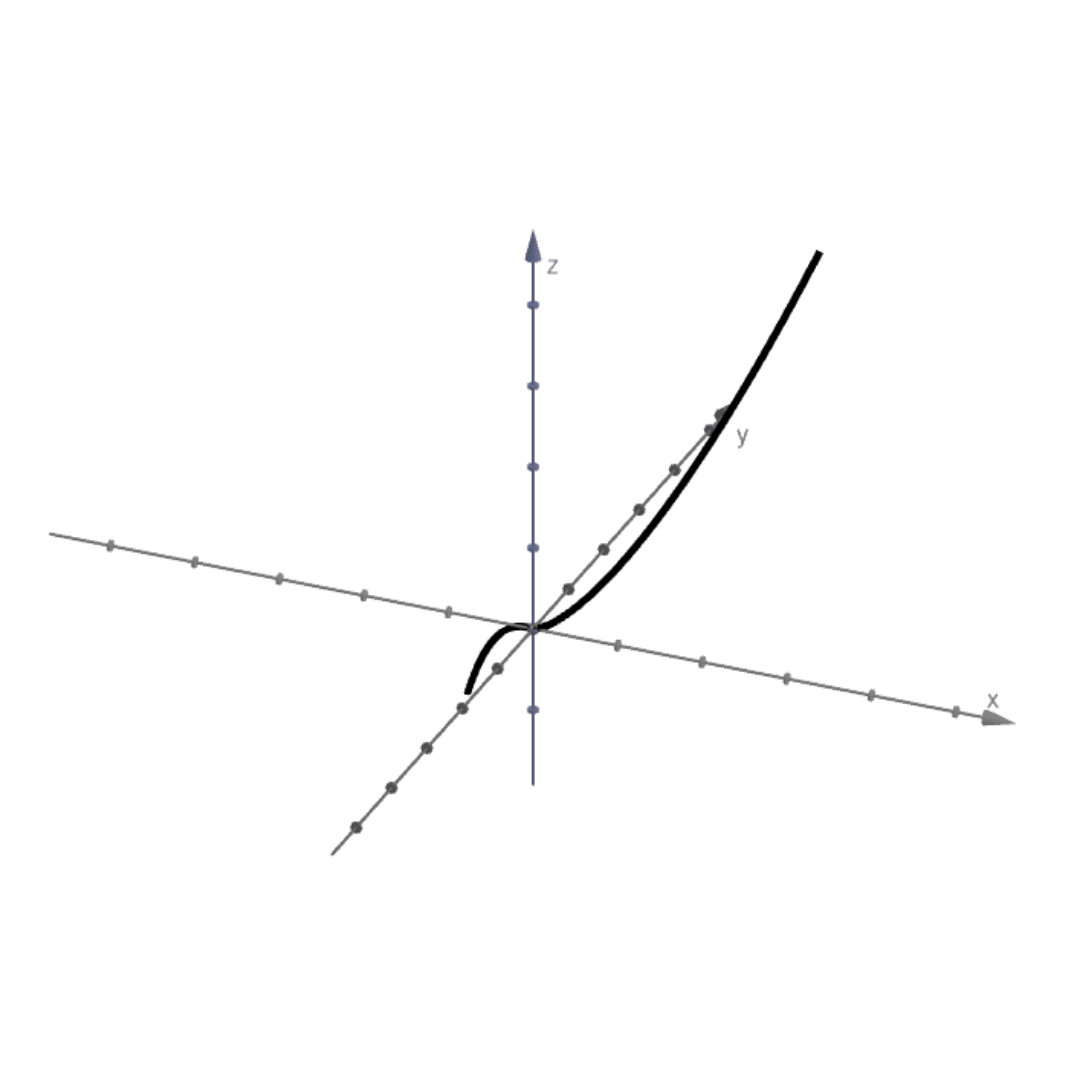
\includegraphics[width=0.3\linewidth]{Imagenes/Curva monomial}
			\caption{Curva monomial $Z(y^2-xz,yz-x^3,z^2-x^2y)$.}
			\label{fig:curva-monomial}
		\end{figure}
	\end{center}
\end{example}

\begin{corollary}\label{analiticoafin}
	Sea $V\subset \cc^n$ una variedad afín no singular de dimensión $r$. Entonces $V$ es una variedad compleja de dimensíon $r$.
\end{corollary}
\begin{proof}
	Sea $p\in V$ un punto albitrario. Como $V$ es no singular de dimensión $r$, por el teorema \ref{teocarlos}, existe una vecindad $U_p\subset V$ de $p$ y polinomios 
	\begin{equation*}
		h_1,\dots,h_{n-r}\in\cc[z_1,\dots,z_n]
	\end{equation*}
	tales que
	\begin{equation*}
		V\cap U_p=\{q\in U_p:h_1(q)=\cdots=h_{n-r}(q)=0\},
	\end{equation*}
	y la matriz jacobiana $(\frac{\partial h_i}{\partial z_j}(p))$ tiene rango $n-r$.\\
	De esto, $0\in \cc^{n-r}$ es un valor regular de la aplicación holomorfa $h=(h_1,\dots,h_{n-r}):U_p\subset\cc^n\to\cc^{n-r}$. Por el ejemplo \ref{interseccioncompleja}, $V\cap U_p$ es una variedad compleja de dimensión
	\begin{equation*}
		n-(n-r)=r.
	\end{equation*}
	Como $p$ fue cualquier punto, obtenemos una cubierta para $V$
	\begin{equation*}
		V=\bigcup_{p\in V}U_p.
	\end{equation*} 
	donde cada $U_p$ es una variedad compleja de dimensión $r$. Finalmente, aplicando el lema \ref{lemacubierta}, $V$ es una variedad compleja de dimensión $r$.
\end{proof}

Dado que toda variedad algebraica afín admite una estructura de variedad compleja, vale la pena preguntarnos si el recíproco es verdad. Es decir, toda variedad compleja se puede realizarse como una variedad algebraica afín. La respuesta a esta cuestión es negativa, pues en primer lugar, las variedades algebraicas afines son conjuntos cerrados de $\cc^n$. De hecho, incluso entre las variedades complejas cerradas en $\cc^n$ existen ejemplos no algebraicas. Esto significa que existen muchas más variedades complejas que variedades algebraicas, por lo que motiva el problema de determinar bajo qué condiciones una variedad compleja admite una realización algebraica.

\begin{example}[Superficie de Riemann no algebraica]\label{graficadelseno}
	Sea
	\begin{equation*}
		X=\{(z,w)\in\mathbb \cc^2:\ w=\sin z\}
	\end{equation*}
	la gráfica de $\sin z$. Entonces $X$ es una superficie de Riemann (de hecho biholomorfa a $\cc$ mediante la proyección $\pi(z,\sin z)=z$) y no es compacta. Supongamos que existe un polinomio no cero $P(z,w)\in\cc[z,w]$ tal que
	\begin{equation*}
		P(z,\sin z)= 0\qquad\text{para todo }z\in\cc.
	\end{equation*}
	Escribamos
	\begin{equation*}
		P(z,w)=\sum_{j=0}^m a_j(z)w^j,\qquad a_j(z)\in\mathbb \cc[z].
	\end{equation*}
	Al evaluar en $w=0$ obtenemos el polinomio $a_0(z)=P(z,0) $. Como $P(z,\sin z)=0$, entonces para todo $z$ tal que $\sin z=0$ (es decir $z=n\pi,\ n\in\mathbb{Z}$) se cumple que $P(z,0)=0$. Así $a_0(z)$ tiene infinitos ceros y por ser un polinomio en $\cc[z]$ debe ser idénticamente cero.
	
	Con lo cual, $w$ divide a $P(z,w)$ en $\cc[z,w]$, es decir existe $P_1\in\cc[z,w] $ tal que
	\begin{equation*}
		P(z,w)=wP_1(z,w)
	\end{equation*}
	Con esto tenemos que
	\begin{equation*}
		0=P(z,\sin z)=\sin zP_1(z,\sin z),
	\end{equation*}
	y como $\sin z$ no es la función cero, entonces $ P_1(z,\sin z)=0$. Usando el mismo razonamiento, obtenemos que $P$ es divisible por $w^k$ para todo $k\geq 1$. Esto sólo es posible si $P$ es el polinomio cero, contradiciendo la hipótesis de que $P\neq0$. Por tanto, $X$ no es algebraica. 
	\begin{figure}[H]
		\centering
		
\includegraphics[width=0.5\linewidth]{Imagenes/Grafica del seno}
		\caption{Gráfica de la función seno}
		%			\caption{La función seno tiene una cantidad infinita de ceros la recta $w=0$. Por lo tanto, si la gráfica del seno fuera algebraica, al intersectar con la recta $w=0$ debería ser algebraica, lo cual no es posible.}
		\label{fig:grafica-del-seno}
	\end{figure}
\end{example}


\begin{definition}
	Sea $V\subset\pp^n$ una variedad algebraica y consideremos $V=\bigcup_{i=0}^n V_i$ la cubierta estandar afín. Definimos la \textbf{dimensión} de $V$ como el máximo de las dimensiones de las variedades afines $V_i\subset\cc^n$.
\end{definition}

En particular, la dimensión es una propiedad local e intrinseca de la variedad  algebraica, sin importar el espacio ambierte donde se encuentre.

\begin{remark}\label{dimcubierta}
	Denotemos por $\cc(V)$ al campo de funciones racionales de la variedad algebraica (afín o proyectiva) $V$. De geometría algebraica (por ejemplo véase \parencite[Cap. 1 Sec. 3]{Harts}) sabemos que si $V$ es afín, entonces
	\begin{equation*}
		\trdeg_{\cc} \cc(V)=\dim V.
	\end{equation*}
	Además, si $V\subset \pp^n$ es una variedad algebraica que no está totalmente contenida en $Z(z_i)$, entonces 
	\begin{equation*}
		\cc(V)\cong \cc(V_i),\qquad \text{con }V_i\text{ como variedad afín}.
	\end{equation*}
	De esta manera, si $V\subset\pp^n$ es una variedad algebraica, entonces para cada $i=0,1,\dots, n$ 
	\begin{equation*}
		\cc(V)\cong \cc(V_i)
	\end{equation*}
	si $V$ no está totalmente contenida en $Z(z_i)$. Asi,
	\begin{equation*}
		\trdeg_{\cc}\cc(V)=\trdeg_{\cc}\cc(V_i)=\dim V_i.
	\end{equation*}
	Por lo tanto, la dimensión de todas las variedades afines $V_i$ es igual a la dimensión de la variedad $V$.
\end{remark}

\begin{definition}
	Sea $V\subset\pp^n$ una variedad algebraica de dimensión $d$ y tomemos su cubierta afín
	\begin{equation*}
		V=\bigcup_{i=0}^n V_i
	\end{equation*}
	Decimos que la variedad $V$ es \textbf{no singular} si todos sus puntos son no singulares en todas las variedades afines. Es decir, las variedades afines $V_i$ son no singulares.
\end{definition}

Por definición, si $V\subset\pp^n$ es no singular, entonces $V$ está cubierta por $n+1$ variedades complejas (especificamente, está cubierto por abiertos en $V$ homeomorfos a una variedad compleja). Aprovecharemos esto para probar que $V$ también es una variedad compleja, pero determinemos antes las propiedades topológicas básicas de las variedades algebraicas.

\begin{lemma}\label{topovariedades}
	Toda variedad algebraica proyectiva es Hausdorff, segundo numerable y compacto (respecto a la topología compleja).
\end{lemma}

\begin{proof}
	Sea $X\subset \pp^n$ una variedad algebraica proyectiva. Notemos que $X$ como subespacio de $\pp^n$ es Hausdorff y segundo numerable. Solo es necesario demostrar que es compacto. Consideremos $X_i=X\cap U_i$ la cubierta afín de $X$. Lo que haremos es demostrar que cada $X_i$ es cerrado. Así, $X$ será cerrado por ser unión finita de cerrados y como $\pp^n$ es compacto, entonces $X$ es compacto.\\
	Como $X$ es variedad algebraica proyectiva, existen $F_k\in\cc[x_0,x_1,\dots,x_n]$ polinomios homogéneos tal que
	\begin{equation*}
		X=Z(F_1,F_2,\dots, F_k)        
	\end{equation*}
	Haremos la prueba para $i=0$, pero es análogo para todo $i=1,\dots, n$.
	Notemos que
	\begin{align*}
		\phi_0(X_0)=Z(f_1,f_2,\dots, f_n)
	\end{align*}
	donde 
	\begin{equation*}
		f_j(x_1,\dots,x_n)=F_j\left(1,x_1,\dots,x_n\right)
	\end{equation*}
	para cada $j=1,2\dots,k$. Esto porque
	\begin{align*}
		\phi_0(X_i)&=\{\phi([1:x_1:\dots:x_n]):[1:x_1.\dots:x_n]\in X_i\}\\
		&=\{(x_1,x_2,\dots,x_n):[1:x_1:\dots:x_n]\in X_i\}\\
		&=\{(x_1,x_2,\dots,x_n):F_j[1:x_1:\dots:x_n]=0, \text{ para toda } j=1,2\dots k\}\\
		&=\{(x_1,x_2,\dots,x_n):f_j(x_1,\dots,x_n)=0, \text{ para toda } j=1,2\dots k\}\\
		&=Z(f_1,f_2,\dots,f_j)\subset \cc^n
	\end{align*}
	Así
	\begin{equation*}
		\phi_0(X_0)=Z(f_1,f_2,\dots,f_j)=\bigcap_{k=1}^jZ(f_k)=\bigcap_{k=1}^jf_k^{-1}(0)
	\end{equation*}
	Por lo tanto, $\phi_0(X_0)$ es cerrado por ser intersección de cerrados y como $\phi$ es un homeomorfismo, entonces $X_0$ es cerrado.
\end{proof}

La conexidad de las variedades algebraicas es un hecho para nada trivial, pero es una propiedad muy importante que necesitamos considerar. Una prueba de esta propiedad se puede consultar en \parencite[Cap. 4 Sec. 4.2]{carlosga} o en \parencite[Cap. VII Sec. 2]{shafarevich2016basic}. Más aún, también podemos verlo como un caso particular del teorema \ref{irreducibleconexo}. Por lo tanto, podemos concluir que:

\begin{theorem}\label{varalg}
	Sea $V\subset\pp^n$ una variedad algebraica no singular de dimensión $r$. Entonces $V$ es una variedad compleja conexa compacta de dimensión $r$.    	
\end{theorem}
\begin{proof}
	Sea $V\subset\pp^n$ una variedad algebraica no singular de dimensión $r$ y consideremos su cubierta estándar 
	\begin{equation*}
		V=\bigcup_{i=0}^n V_i.
	\end{equation*}
	Supongamos que $V\not\subset Z(z_i)$ para todo $i=0,1,\dots,n$. Por la observación \ref{dimcubierta}, las variedades afines $V_i$ dimensión $r$. Luego, por definición de no singular, las $V_i$ son no singulares. De esta manera, por el corolario \ref{analiticoafin}, las variedades afines $V_i$ tienen estructura de variedad compleja de dimensión $r$.\\
	Por el lema \ref{lemacubierta}, como $V$ está cubierto por las variedades complejas $V_i$, concluimos que $V$ tiene estructura de variedad compleja de dimensión $r$.\\
	Ahora, si $V$ está totalmente contenida en algún $Z(z_i)$, digamos $i=0$, entonces $V_i=\emptyset$. Por lo que
	\begin{equation*}
		V=\bigcup_{i=0}^n V_i=\bigcup_{i=1}^n V_i
	\end{equation*}
	y la demostración sigue siendo válida.
	
	Por el lema \ref{topovariedades}, $V$ es compacta. Además, la conexidad de $V$ se sigue de la irreducibilidad de las variedades algebraicas proyectivas (véase la discusión previa al teorema). Por lo tanto, $V$ es una variedad compleja conexa y compacta de dimensión r.
\end{proof}

\section{Lo analítico en el mundo algebraico}

Veamos las consecuencias que occuren de que las variedades algebraicas son variedades complejas.

\begin{example}
    Sobre una variedad algebraica (afín o proyectiva) las funciones regulares son holomorfas y las funciones racionales son meromorfas.
\end{example}

Podriamos pensar que una función racional sea meromorfa en un punto y al mismo tiempo sea regular en el mismo punto. Sin embargo, esto no puede pasar:
\begin{theorem}
    Sea $V\subset\pp^n$ una variedad algebraica lisa y $\phi\in K(V)$. Si $f$ es holomorfa en $p$, entonces $f$ es regular en $p$.
\end{theorem}

Nos gustaría relacionar directamente las funciones regulares y holomorfas. Sin embargo, ambas nociones están definidas en topología distintas y estructuras distintas. La estructura algebraica dada por ceros de polinomios y la topología de Zariski, mientras y la estructura holomorfa (también llamada analítica) dadas por cartas holomorfas y la topología compleja. \\
Pero sí podemos demostrar la correspondencia con las funciones meromorfas y racionales definidas en toda la variedad. 

\begin{theorem}
    Sea $V\subset\pp^n$ una variedad proyectiva lisa. Entonces 
    \begin{equation*}
        K(V)=\mathcal{K}(V)
    \end{equation*}
    Es decir, las funciones racionales y meromorfas globales coinciden.
\end{theorem}

\begin{propo}
    Toda aplicación holomorfa $f:V\to W$ entre variedades algebraicas proyectivas lisas es regular.
\end{propo}

\begin{propo}
    Dos variedades algebraicas son isomorfas si, y  solo si, son biholomorfas.
\end{propo}

\begin{theorem}
    Toda variedad compleja compacta conexa dentro de una variedad algebraica lisa es una variedad algebraica lisa.
\end{theorem}



	
	\chapter{Encaje al proyectivo}\label{cap2}

	Encajar variedades en otros espacios juega un papel importante en la geometría diferencial, pues permiten trabajar variedades muy abstractas como subvariedades de algún espacio ya conocidos. Existen varios resultados clásicos en esta dirección, por ejemplo:
	
    \begin{theorem}[Teorema del Encaje de Whitney]
        Toda variedad diferenciable suave de dimensión $n$ admite un encaje suave y propio a $\rr^{2n+1}$.
    \end{theorem}
    
    Aunque este resultado no siempre proporciona la mejor cota posible para la dimensión del espacio ambiente\footnote{En general, $2n$ es suficiente para un encaje suave, pero es más complicado de probar. Además, una superficie real orientable puede encajarse en $\rr^3$, mientras que una no orientable puede encajarse, en general, en $\rr^4$.}, su importancia conceptual es fundamental, pues permite considerar toda variedad suave real como un objeto concreto dentro de algún espacio euclidiano $\rr^N$. Esta perspectiva hace posible abordar numerosas cuestiones geométricas y topológicas mediante herramientas del cálculo y de la geometría clásica \parencite[Ver Cap.~6]{lee2003smooth}.
    
    En el contexto de la geometría compleja la situación es sustancialmente más restrictiva (véase el ejemplo \ref{encajeccn}). La inexistencia general de un teorema de encaje holomorfo en espacios afines complejos podría parecer, en principio, una limitación.
    
    No obstante, conviene recordar el caso de las variedades algebraicas. Estas son variedades complejas que se realizan de manera natural como subvariedades del espacio proyectivo complejo. Dicho espacio ambiente posee propiedades topológicas y algebraicas de gran relevancia, como la topología de Zariski y la compacidad, que resultan extremadamente útiles desde el punto de vista geométrico.
   
    \begin{example}
        Consideremos el polinomio $f(x,y)=y^2-x^3+x\in\cc[x,y]$, el cual tiene grado $3$, es irreducible y no singular. Entonces 
        \begin{equation*}
            Z(f)=\{(x,y)\in\mathbb{C}^2: f(x,y)=0\}
        \end{equation*}
        es una curva compleja.
        \begin{figure}[H]
        	\centering
        	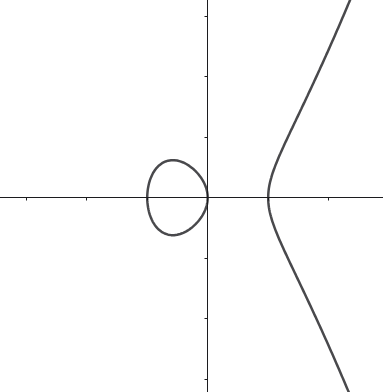
\includegraphics[width=0.25\linewidth]{Imagenes/Curva eliptica afin}
        	\caption{Curva algebraica afín $Z(y^2-x^3+x)$.}
        	\label{fig:curva-eliptica-afin}
        \end{figure}
        Ahora consideremos la homogeneización del polinomio $f(x,y)$ dada por
        \begin{equation*}
            F(X,Y,Z)=Z^3\left( \left(\frac{Y}{Z}\right)^2-\left(\frac{X}{Z}\right)^3+\frac{X}{Z}\right)=Y^2Z-X^3+XZ^2\in\cc[X,Y,Z].
        \end{equation*}
        Este polinomio es homogéneo de grado $3$ y su conjunto de ceros
        \begin{equation*}
            X=Z(F)=\{[X:Y:Z]\in\pp^2:F(X,Y,Z)=0\}
        \end{equation*}
        es una curva algebraica proyectiva. Ahora estudiemos sus puntos al infinito.\\
        Si $Z=0$, entonces $-X^3=0$. Esto implica que $X=0$. Por lo que el único punto al infinito es 
        \begin{equation*}
            [0:1:0].
        \end{equation*}
        Queremos ver ahora que $F$ no es singular en $[0:1:0]$. Las parciales de $F$ están dadas por
        \begin{equation*}
            F_X=-3X^2+Z^2,\qquad F_Y=2XZ,\qquad F_Z=Y^2+2XZ.
        \end{equation*}
        Con lo que, evaluando en el punto $[0:1:0]$, tenemos que
        \begin{equation*}
            F_X(0,1,0)=0,\qquad F_Y(0,1,0)=0,\qquad F_Z(0,1,0)=1.
        \end{equation*}
        Como todas las parciales son no cero, la curva es no singular en ese punto. Como $X$ es una curva proyectiva no singular, posee estructura natural de superficie de Riemann. Además, la fórmula de Plücker
        \begin{equation*}
        	\frac{(d-1))(d-2)}{2},\qquad \text{donde }d\text{ es el grado del polinomio }F
        \end{equation*}
        nos muestra que la curva tiene género 1. (véase figura \ref{fig:toro}).
        
        Más aún, dado que $X\subset\pp^2$ entonces $X$ es una variedad compleja que vive dentro del plano proyectivo $\pp^2$. Más adelante veremos que, de hecho, es una subvariedad compleja y subvariedad analítica de $\pp^2$.
    \end{example}
    
    Considerando el caso de las variedades algebraicas proyectivas, surge de manera natural la siguiente pregunta: \textit{¿Qué variedades complejas pueden realizarse como subvariedades de algún espacio proyectivo complejo?} Tan sencilla como aparentemente específica, esta pregunta constituye la motivación central de este trabajo. Su respuesta, sin embargo, dista de ser inmediata y conduce a resultados considerablemente más profundos de lo que su formulación inicial pueda sugerir.
    
\section{Encaje Holomorfo}
	
	Para de responder la pregunta anterior, introduciremos las nociones necesarias para formular con precisión el problema.
	
	Un \textit{encaje holomorfo} es una aplicación holomorfa que preserva la estructura compleja, la topología y la geometría exterior de una variedad compleja. El estudio de estos encajes al espacio proyectivo nos revela demasiada estructura de las variedades que los admiten, viendo que son bastante escasas los espacios que admiten estos encajes. En esta sección vamos a introducir el concepto de encaje holomorfo para analizar sus propiedades básicas, así como algunos ejemplos y contraejemplos relevantes.
	    
    \begin{definition}
        Sean $M$ y $N$ variedades complejas de dimensión $n$ y $k$ respectivamente. Una aplicación holomorfa $f:N\to M$ es un \textbf{encaje holomorfo} si satisface:
        \begin{enumerate}
            \item $f$ es inyectiva.
            \item (\textbf{Encaje topológico}) $f$ es un homeomorfismo con su imagen, es decir, $f:N\to f(N)$ es biyectiva, continua y con inversa continua ($f(N)$ lleva la topología del subespacio de $M$).
            \item Para cada $p\in N$, existen cartas $(U,\varphi)$ alrededor de $f(p)\in M$ y $(V,\psi)$ alrededor de $p\in N$ tales que $f(V)\subset U$ y en coordenadas
            \begin{equation*}
                \varphi\circ f\circ\psi^{-1}(z_1,\cdots,z_k)=(z_1,\cdots,z_k,0\cdots,0)\in\cc^n.
            \end{equation*}.
        \end{enumerate}
        Notemos que la condición $3$ nos indica que $f$, localmente, coincide con la inclusión $\cc^k\hookrightarrow\cc^n$, $z\mapsto (z,0)$.
    \end{definition}

    \begin{example}[Gráfica de una aplicación holomorfa]
    	Sea $N$ una variedad compleja de dimensión $n$ y $g:N\to\cc^{m}$ una aplicación holomorfa. Consideremos la aplicación
    	\begin{align*}
    		f:N\longrightarrow N\times\cc^{m}\\
    		z\mapsto(z,g(z)).
    	\end{align*}
    	Notemos que $f$ es una aplicación holomorfa pues cada una de sus componentes es holomorfa. Además, es inyectiva pues es la identidad en la primera entrada.\\
    	Luego, la aplicación inversa $f^{-1}:f(N)\to N$ está dada por
    	\begin{equation*}
    		f^{-1}(z,g(z))=z
    	\end{equation*}
    	la cual es continua. Por lo que $f:N\to f(N)$ es un homeomorfismo.\\ 
    	Consideremos una carta $(U,\varphi)$ una carta de $N$, $\varphi:U\to V\subset\cc^n$. Definamos la aplicación holomorfa $G:=g\circ \varphi^{-1}:V\to\cc^m$. De esta manera, obtenemos el biholomorfismo 
    	\begin{align*}
    		\Psi:V\times \cc^m\longrightarrow V\times \cc^m\\
    		(z,w)\mapsto (z,w-G(z)),
    	\end{align*}
    	pues su inversa es la aplicación $(z,w)\mapsto (z,w+G(z))$. Con lo cual, 
    	\begin{equation*}
    		\Psi(\varphi(U)\times\cc^m\cap f(U))=\{(z,0):z\in V\cap\varphi(U)\}=V\times\{0\}.
    	\end{equation*}
    	Definamos entonces la carta $\psi=\Psi\circ (\varphi\times \text{id})$ se cumple que
    	\begin{equation*}
    		\psi\circ f\circ \varphi^{-1}:V\to V\times\cc^m\subset \cc^{n+m} 
    	\end{equation*}
    	está dada por
    	\begin{equation*}
    		\psi\circ f\circ\varphi^{-1}(z)=(z,0)\in\cc^n\times\cc^m.
    	\end{equation*}
    	Por lo tanto, se cumple la definición de encaje holomorfo.\\
        Intuitivamente, $f$ está \enquote{dibujando} a la variedad $N$ dentro de $N\times\cc^m$ sin doblarla y sin autointersectarla.
        \begin{figure}[H]
        	\centering
        	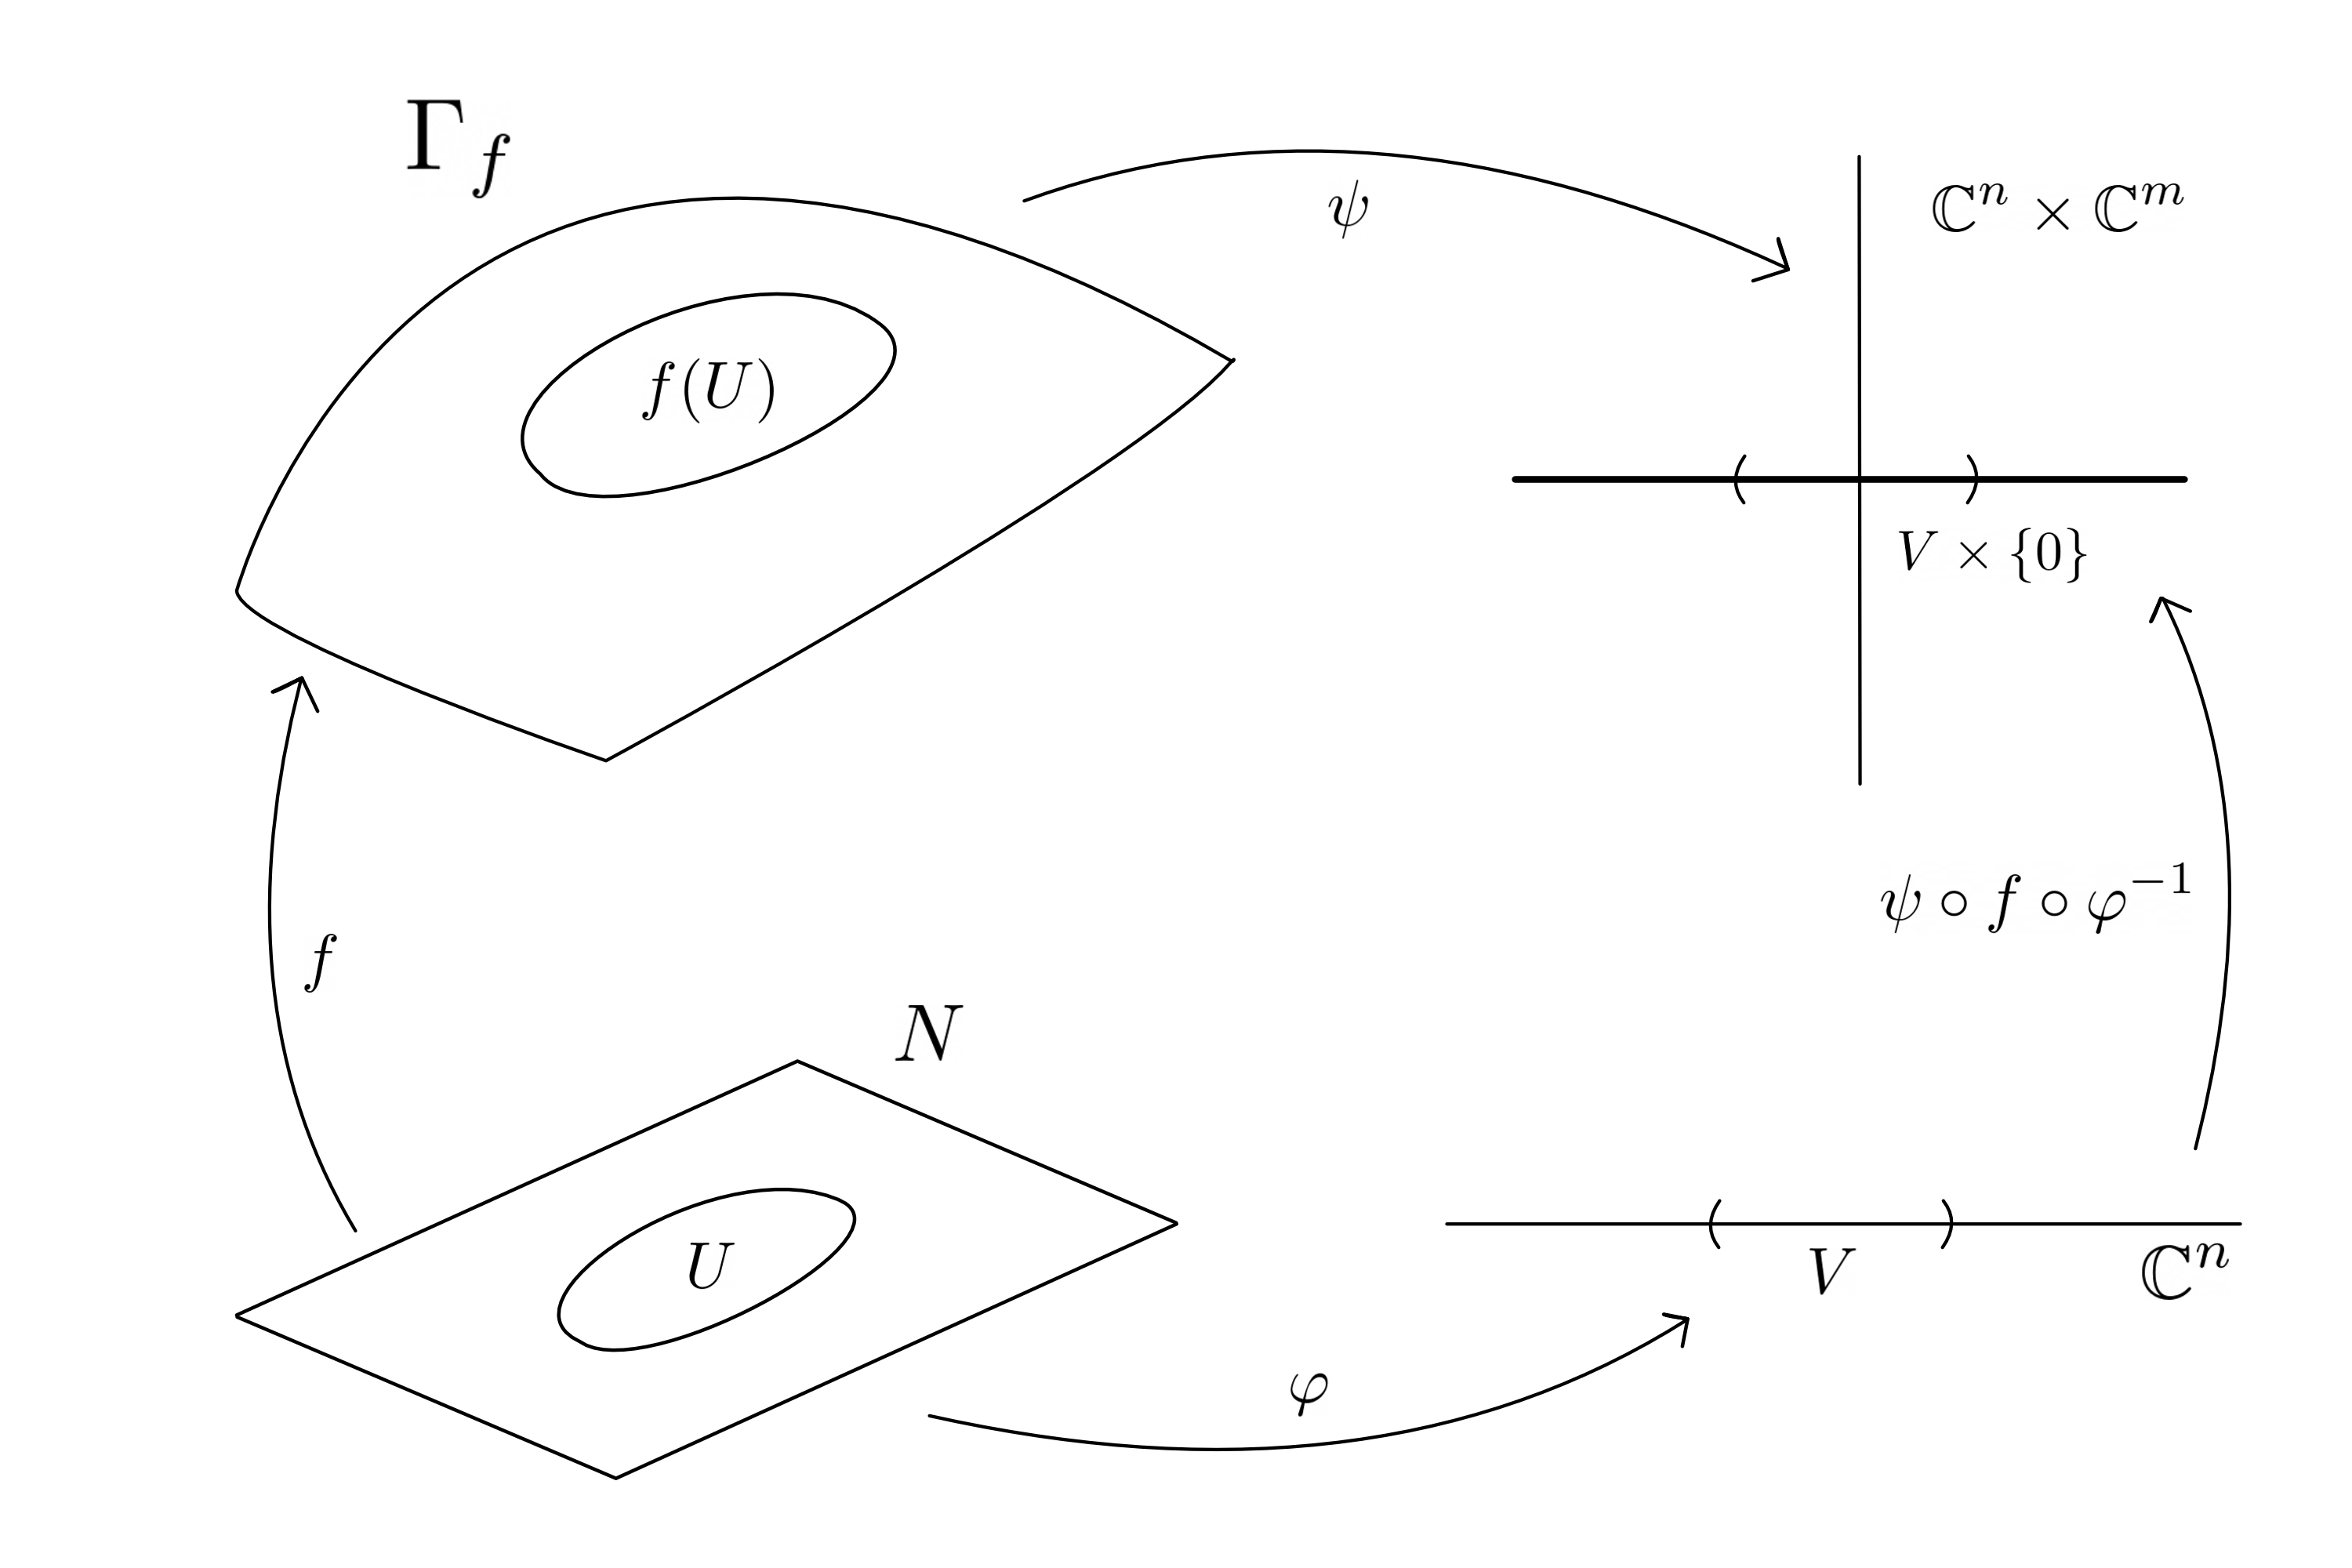
\includegraphics[width=0.6\linewidth]{Imagenes/Encaje de grafica}
        	\caption{Diagrama del encaje dada por una aplicación holomorfa.}
        	\label{fig:encaje-de-grafica}
        \end{figure}
         
    \end{example}
    
    
    \begin{definition}[Subvariedad compleja]
        Una variedad compleja $N$ es una \textbf{subvariedad compleja} (cerrada) de dimensión $k$ de una variedad compleja $M$, con $\dim M=n$, si $N\subset M$ es un subconjunto cerrado y existe un atlas holomorfo $\{U_i,\varphi_i\}$ de $M$ tal que 
        \begin{equation*}
            \varphi_i(U_i\cap N)\cong \varphi_i(U_i)\cap\cc^k
        \end{equation*}
        donde $\cc^k$ está encajado en $\cc^n$ por $z\mapsto (z,0)$. Definimos la \textbf{codimensión} de $N$ en $M$ como
        \begin{equation*}
            \mathrm{codim}N:=\dim M-\dim N=n-k.
        \end{equation*}
    \end{definition}
    
    \begin{remark}\label{subvariedadesporecuaciones} $ $
    	\begin{enumerate}
    		\item Si $N$ es una subvariedad compleja de $M$ y la inclusión $\iota:N\hookrightarrow M$ es propia (o $N$ es compacto), entonces $\iota$ es un encaje holomorfo. Más aún, si $f:N\to M$ es un encaje holomorfo, entonces $f(N)$ es una subvariedad compleja de $M$.
    		\item Consideremos una variedad compleja $M$ y una subvariedad compleja $N\subset M$ de dimensión $k$. Por definición, para todo punto $p\in N$ existe una carta holomorfa $(U,\varphi)$ de $M$ tal que, después de identificar $\cc^k$ con el subespacio lineal
    		\begin{equation*}
    			\cc^k\times\{0\}\subset\cc^n
    		\end{equation*}
    		se cumple que
    		\begin{equation*}
    			\varphi(U\cap N)=\varphi(U)\cap (\cc^k\times \{0\}).
    		\end{equation*}
    		Si tomamos las coordenadas $z_1,\dots,z_n$ de $\cc^n$, entonces en dicha carta, $U\cap N$ queda descrita por las ecuaciones 
    		\begin{equation*}
    			z_{k+1}=\cdots=z_n=0.
    		\end{equation*}
    		Equivalentemente
    		\begin{equation*}
    			U\cap N=\bigcap_{j=k+1}^n f_j^{-1}(0)=Z(f_{k+1},\dots f_n),
    		\end{equation*}
    		donde $f_j=z_j\circ \varphi$. Por lo tanto, localmente $N$ es una subvariedad de intersección completa descrita por $n-k$ funciones holomorfas.
    	\end{enumerate}
    \end{remark}

	\begin{example}\label{algsonsubvariedades}
		Toda variedad algebraica no singular es una subvariedad compleja del espacio proyectivo. 
			Sea $V\subset\pp^n$ una variedad algebraica proyectiva no singular. Por definición, existe una cantidad finita de polinomios homogéneos $F_1,\dots,F_r\in \cc[x_0,\dots,x_n]$ tal que
			\begin{equation*}
				V=Z(F_1,\dots,F_r).
			\end{equation*}
			Fijemos una carta afín $U_i\subset \pp^n$
			y consideremos las coordenadas afines
			\begin{equation*}
				z_j=\frac{x_j}{x_i},\qquad j\neq i.
			\end{equation*}
			En esta carta, las ecuaciones homogéneas se transforman en ecuaciones polinómicas
			\begin{equation*}
				f_\ell(z_1,\dots,\widehat{z_i},\dots,z_n)=0,
				\qquad \ell=1,\dots,r,
			\end{equation*}
			donde cada $f_\ell$ es una función holomorfa sobre $U_i\cong \cc^n$. De esta manera,
			\begin{equation*}
				V\cap U_i=\{p\in U_i : f_1(p)=\cdots=f_r(p)=0\}
			\end{equation*}
			Sea $p\in V\cap U_i$. Como $V$ es no singular, el jacobiano de las ecuaciones tiene rango máximo igual a la codimensión de $V$ en $\pp^n$. Por el teorema de la función implícita \ref{funcionimplicita}, existen coordenadas holomorfas locales
			\begin{equation*}
				(w_1,\dots,w_n)
			\end{equation*}
			en una vecindad de $p$ tales que
			\begin{equation*}
			 V\cap U_i=Z(w_{k+1},\dots w_n).
			\end{equation*}
			Por lo observación \ref{subvariedadesporecuaciones}, $V$ es una subvariedad compleja de $\pp^n$, y la estructura compleja inducida coincide con la obtenida mediante las cartas holomorfas de $\pp^n$.
	\end{example}

	\begin{example}[Biholomorfismo que no es encaje]
		Sea $f:\cc\to\cc^*\times\cc^*$ la aplicación holomorfa
		\begin{equation*}
			f(z)=(e^z,e^{\alpha z}),
		\end{equation*}
		donde $\alpha\in\rr\setminus\mathbb{Q}$. Vamos a probar que $f$ es biholomorfa a su imagen. 
		
		Para la inyectividad, supongamos que $f(z)=f(w)$. Entonces
		\begin{equation*}
			e^{z-w}=1,\qquad e^{\alpha(z-w)}=1.
		\end{equation*}
		Así, existen $n,m\in \zz$ tales que
		\begin{equation*}
			z-w=2\pi i n,\qquad \alpha(z-w)=2\pi im.
		\end{equation*}
		Si $n\neq 0$, entonces $\alpha=m/n\in\mathbb{Q}$ lo cual es una contradicción. De esta manera, $n=0$ e implica que $z=w$. Por tanto, $f$ es inyectiva.
		
		Fijemos $z_0\in\cc$ y pongamos
		\begin{equation*}
			p=f(z_0).
		\end{equation*}
		Como la primera coordenada de $p=(p_1,p_2)$ es un punto en $\cc^*$, existe una vecindad $V$ de $p_1=e^{z_0}$ donde existe una rama del logaritmo
		\begin{equation*}
			\log_V:V\longrightarrow\cc.
		\end{equation*}
		Entonces, en una vecindad suficientemente pequeña de $p$ dentro de la imagen
		\begin{equation*}
			f^{-1}(w_1,w_2)=\log_V(w_1).
		\end{equation*}
		Con esto, $f^{-1}$ es holomorfa alrededor de cada punto de la imagen. Es decir, la aplicación
		\begin{equation*}
			f^{-1}:f(\cc)\longrightarrow\cc
		\end{equation*}
		es holomorfa. Con esto, $f$ es biholomorfa con su imagen. 
		
		Para probar que $f$ no es encaje, vamos a probar que $f:\cc\to f(\cc)$ no es un homeomorfismo si $f(\cc)$ lleva la topología del subespacio. 
		
		Consideremos la sucesión 
		\begin{equation*}
			z_n=2\pi in.
		\end{equation*} 
		Entonces
		\begin{equation*}
			f(z_n)=(1,e^{2\pi i\alpha n}).
		\end{equation*}
		Como $\alpha$ es irracional, la sucesión $\{e^{2\pi i\alpha n}\}$ es densa en $S^1$. Por lo que, existe una subsucesión $n_k$ tal que
		\begin{equation*}
			e^{2\pi i\alpha n_k}\longrightarrow 1.
		\end{equation*} 
		De esta manera, 
		\begin{equation*}
			f(z_{n_k})\longrightarrow (1,1)=f(0).
		\end{equation*}
		Sin embargo, $z_{n_k}=2\pi i n_k$ no converge a $0\in\cc$. Por lo que, la inversa $f^{-1}:f(\cc)\to\cc$ no es continua como espacios métricos, es decir, $f:\cc\to f(\cc)$ no es un homeomorfismo con la topología del subespacio de $f(\cc)$.
		\begin{figure}[H]
			\centering
			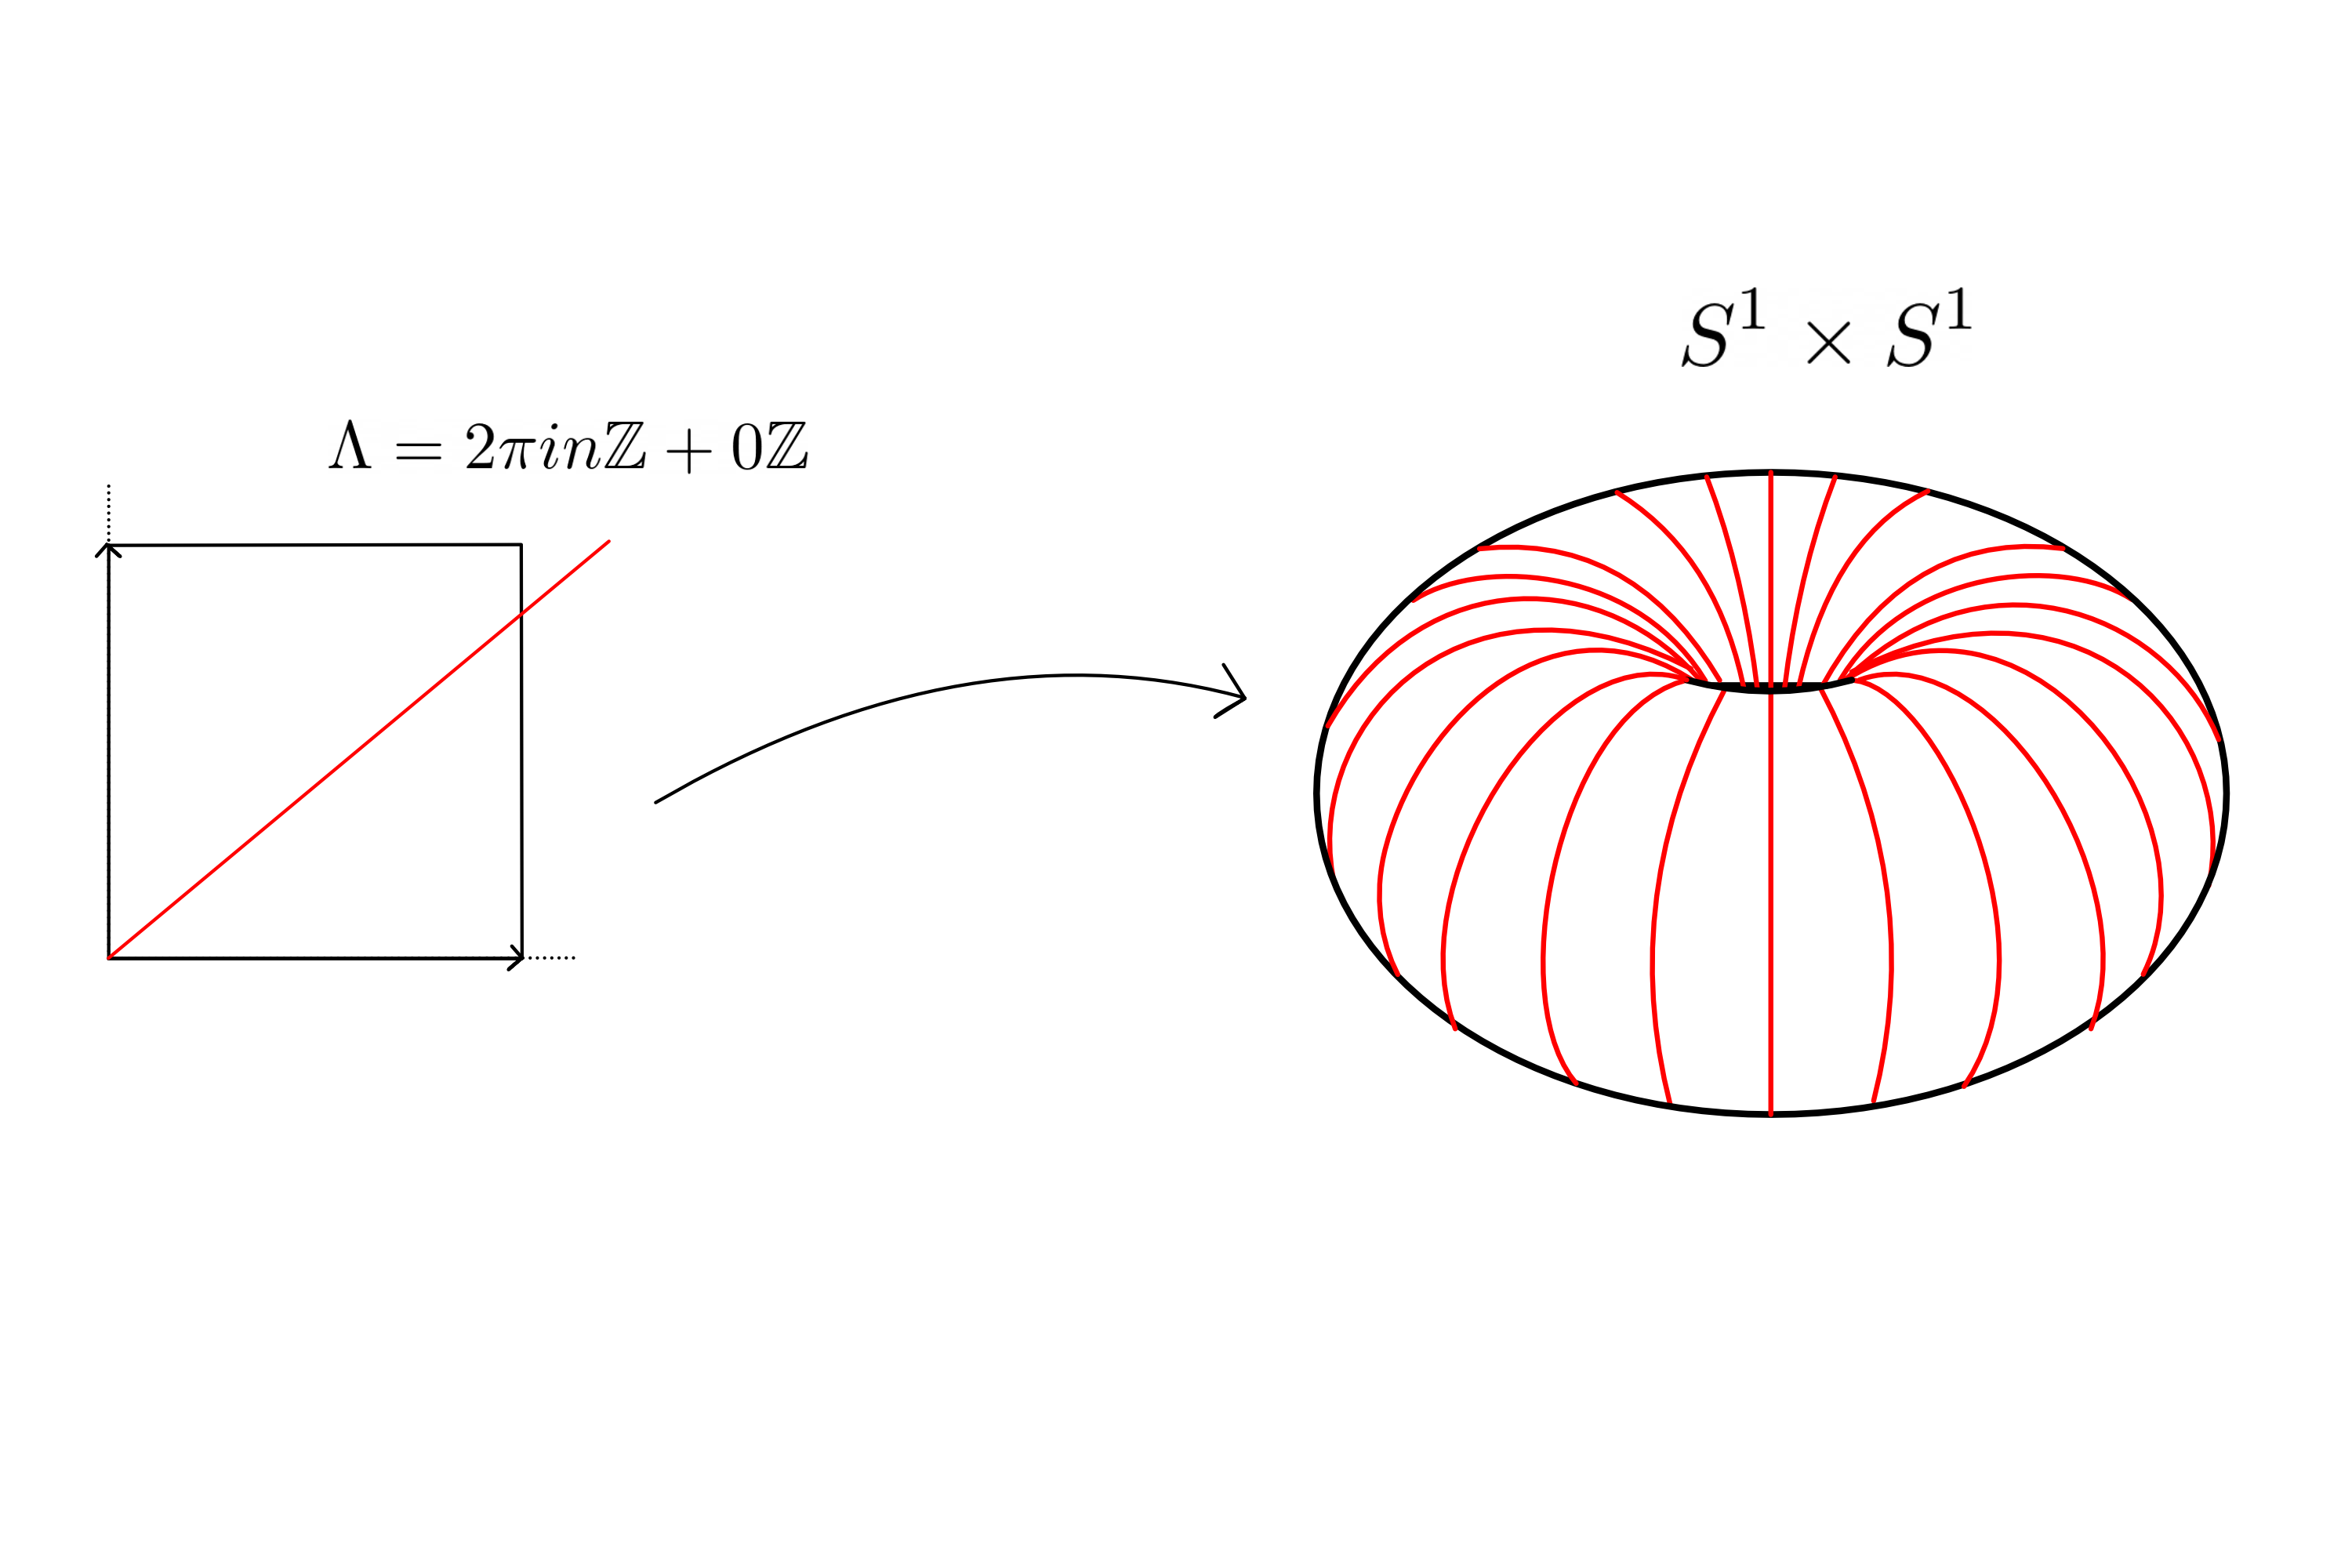
\includegraphics[width=0.7\linewidth]{Imagenes/biholomorfismo}
			\caption{Imagen de la recta imaginaria enrollada de forma densa sobre el toro (enrollamiento irracional sobre el toro).}
			\label{fig:biholomorfismo}
		\end{figure}
		
	\end{example}
	
    Como mencionabamos, el teorema de Whitney es un resultado general importante en la geometría diferencia real, pero no podemos tener un análogo directo en geometría compleja.
    
    \begin{example}\label{encajeccn}
        \textbf{No existen} subvariedades complejas compactas de $\cc^n$ de dimensión no cero. Ya que si $M\subset\cc^n$ es una subvariedad compleja compacta, entonces cada funcion de $\cc^n$ coordenada (proyección) $z_j$\footnote{Como $M$ es subvariedad, la inclusión $i:M\to \cc^n$ es holomorfa. Si $\pi_j:\cc^n\to\cc$ es la proyección a la $j$-ésima entrada, la función de $\cc^n$ coordenada $z_j=\pi_j\circ i:M\to \cc$ es una función holomorfa por ser composición de aplicaciones holomorfas.} restringida a $M$ es una función holomorfa global de $M$. Por el teorema \ref{holomorfasglobal}, $z_j$ es constante en cada componente conexa de $M$. Por lo que la inclusión $i:M\to\cc^n$ es constante en cada componente conexa de $M$. Con lo cual, cada componente conexa de $M$ consta de un único punto. Como $M$ es compacto, sólo puede tener un número finito de componentes conexas. En consecuencia, $M$ es un conjunto finito y, por tanto, tiene dimensión 0.
    \end{example}
    
    Ahora vamos a probar un resultado que nos ayudará a comprobar que una aplicación sea un encaje holomorfo. 
    
    \begin{propo}\label{encajesubvariedades}
    	Una aplicación holomorfa $f:M\to N$ es un encaje holomorfo si, y solo si, $f:M\to f(M)$ es un biholomorfismo y $f(M)\subset N$ es una subvariedad compleja.
    \end{propo}
    \begin{proof}
    		Primero, supongamos que $f:M\to N$ es un encaje. Por la condición de encaje topológico, $f:M\to f(M)$ es un homeomorfismo. En particular, la inversa $f^{-1}:f(M)\to M$ es continua.
    		
    		Tomemos $p\in M$ y sea $q=f(p)\in N$. Por la condición $(3)$ de encaje, existen cartas holomorfas $(V,\psi)$ alrededor de $q$ y $(U,\varphi)$ alrededor de $p$ tales que $f(U)\subset V$ y
    		\begin{equation*}
    			\psi\circ f\circ \varphi^{-1}(z_1,\dots,z_k)=(z_1,\dots,z_k,0,\dots,0)\in \cc^n.
    		\end{equation*}
    		Como $f$ es un homeomorfismo, $f(U)$ es abierto en $f(M)$ y $f(M)$ lleva la topología de subespacio, al reducir $V$ si es necesario podemos suponer que $V\cap f(M)=f(U)$. Entonces, en este abierto la inversa de $f$ se escribe en coordenadas como la proyección sobre las primeras $k$ coordenadas:
    		\begin{equation*}
    			\varphi\circ f^{-1}\circ \psi^{-1}(w_1,\dots,w_n)=(w_1,\dots,w_k),
    			\qquad (w_1,\dots,w_n)\in \psi(V\cap f(M)).
    		\end{equation*}
    		Esta expresión es holomorfa. Como $p$ era arbitrario, $f^{-1}$ es holomorfa en todo $f(M)$. Por tanto, $f:M\to f(M)$ es un biholomorfismo.
    		
    		Para ver que $f(M)$ es una subvariedad compleja de $N$, observemos que las mismas cartas satisfacen
    		\begin{equation*}
    			\psi(V\cap f(M))=\psi(V)\cap (\cc^k\times \{0\}).
    		\end{equation*}
  			Es decir, $f(M)$ es una subvariedad compleja de $N$.
  			
  			Ahora, supongamos que $f:M\to f(M)$ es un biholomorfismo y $f(M)$ es subvariedad compleja. Entonces es inmediato que $f:M\to f(M)$ es un encaje topológico donde $f(M)$ lleva la topología del subespacio. 
  			
  			Sea $p\in M$ y $q=f(p)\in N$. Como $f(M)$ es una subvariedad compleja, existe una carta holomorfa $(V,\psi)$ de $q$ tal que
  			\begin{equation*}
  				\psi(V\cap f(M))=\psi(V)\cap (\cc^k\times \{0\}).
  			\end{equation*} 
  			Sea $U:=f^{-1}(V)\subset M$. Entonces $f|_U:U\to V\cap f(M)$ sigue siendo un biholomorfismo. Consideremos la proyección a las primeras $k$ entradas
  			\begin{align*}
  				&\pi:\cc^n\longrightarrow \cc^k\\
  				(z_1,\dots,z_k&,\dots,z_n)\mapsto (z_1,\dots, z_k).
  			\end{align*} 
  			Definamos entonces 
  			\begin{equation*}
  				\varphi:=\pi\circ \psi\circ f|_U:U\longrightarrow\cc^k.
  			\end{equation*}
    		Como $\psi(f(V))\subset \cc^k\times \{0\}$, la aplicación restringida a $\pi$ sigue siendo un biholomorfismo sobre $\cc^k$. Por lo que, $\varphi$ es una carta holomorfa alrededor de $p$.
    		
    		Además, para todo $z\in\varphi(U)\subset\cc^k$, 
    		\begin{equation*}
    			\psi\circ f\circ \varphi^{-1}(z)=(z,0)\in\cc^n.
    		\end{equation*}
    		Por lo tanto, $f$ satisface la propiedad $(3)$ y concluimos que $f$ es un encaje holomorfo. 
    \end{proof}
    
    Un biholomorfismo sobre su imagen solo exige que existe una inversa holomorfa entre conjuntos, pero no garantiza que el dominio tenga la estructura analítica de la subvariedad imagen. En otras palabras, un encaje holomorfo es un biholomorfismo sobre su imagen cuya imagen es una subvariedad compleja. 
    
%    \begin{example}
%        Consideremos la aplicación holomorfa $f:\cc\to\pp^1$ dada por 
%        \begin{equation*}
%        	f(z)=[z:1]
%        \end{equation*}
%      	Notemos que $f$ es un homeomorfismo pues es la inversa de una carta afín de $\pp^1$. Así, determina un biholomorfismo entre $\cc$ y $\pp^1\setminus \{[1:0]\}$. Sin embargo, $\pp^1\setminus\{[1:0]\}$ no es una subvariedad compleja de $\pp^1$. Por lo tanto, $f$ no es un encaje holomorfo.
%      	\begin{figure}[H]
%      		\centering
%      		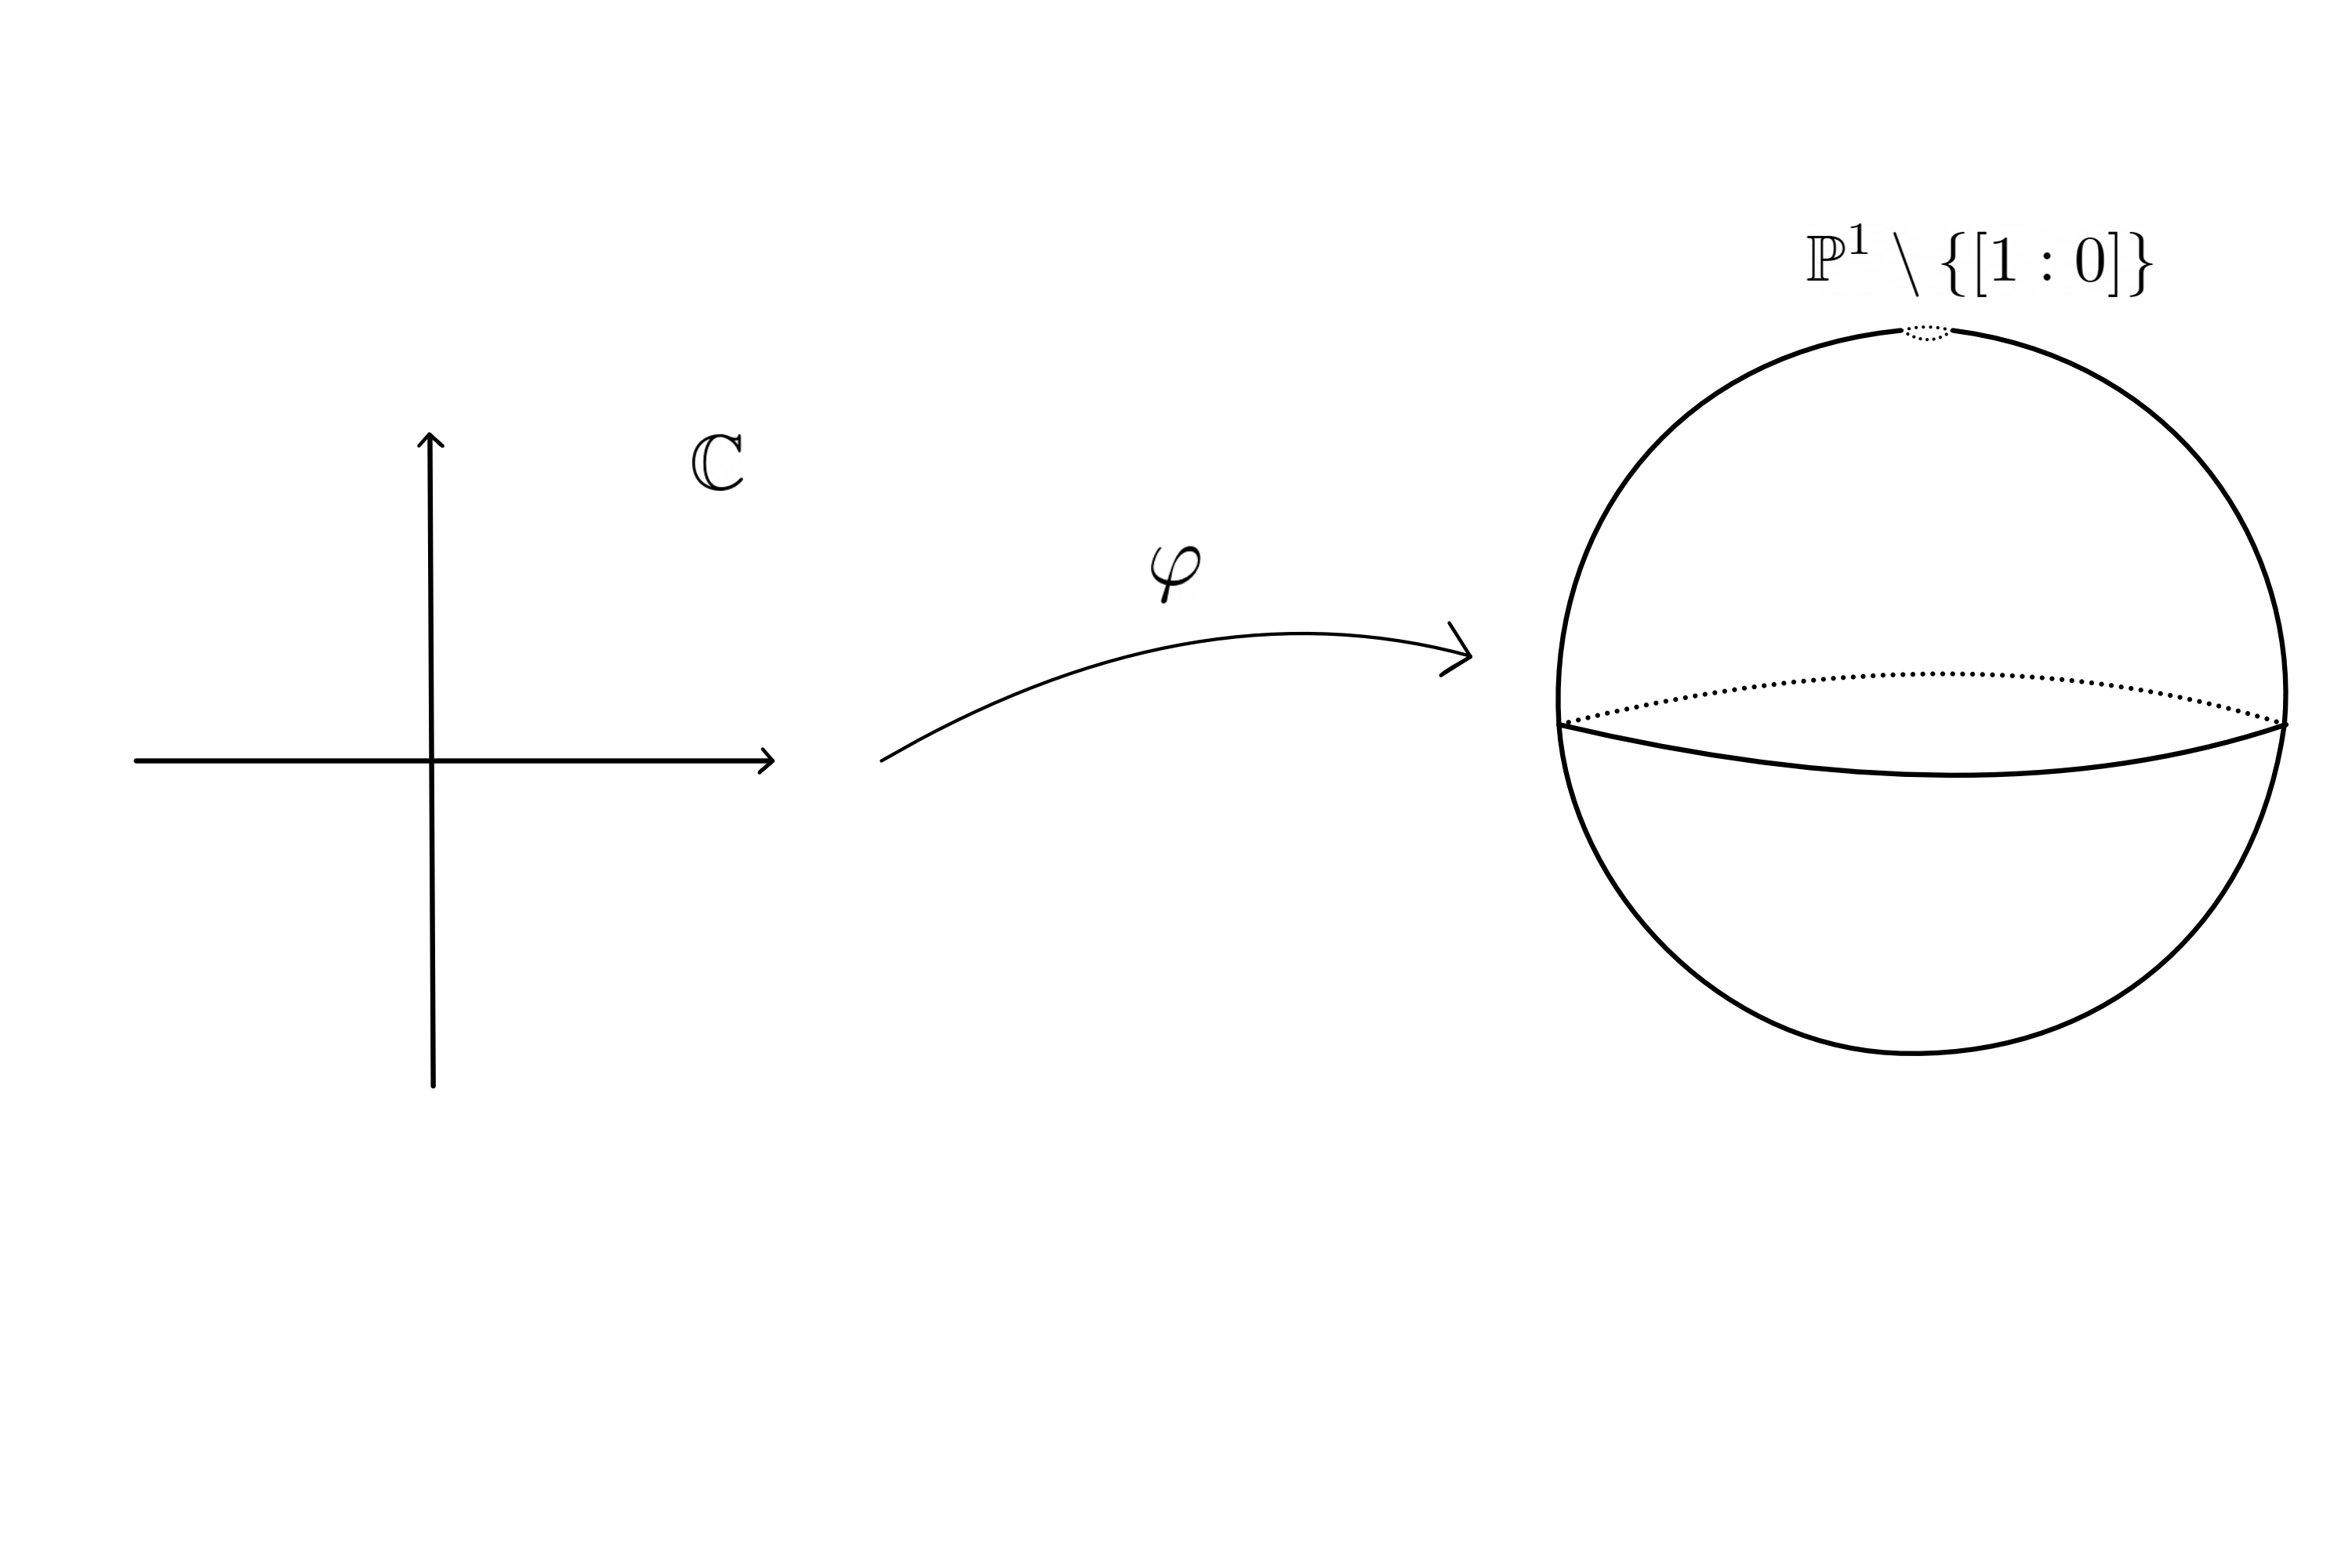
\includegraphics[width=0.5\linewidth]{Imagenes/no encaje a P1}
%      		\caption{Inmersión de $\cc$ en $\pp^1$.}
%      		\label{fig:no-encaje-a-p1}
%      	\end{figure}
%      	
%    \end{example}
   	
   	Un encaje puede entenderse, en este contexto, como una manera de \enquote{incrustar} una variedad en otra sin perder su estructura compleja. En particular, nos interesan los encajes en espacios proyectivos, cuya importancia será gracias al teorema de Chow, que abordaremos en el siguiente capítulo. Finalmente, introduzcamos la noción de una variedad que admita un encaje al espacio proyectivo.
   	
   	\begin{definition}
   		Una variedad compleja $M$ se dice \textbf{proyectiva} si admite un biholomorfismo sobre una subvariedad compleja de algún espacio proyectivo complejo. Equivalentemente por la proposición anterior, $M$ es proyectiva si admite un encaje a un espacio proyectivo.
   	\end{definition}
   	
   	\subsection{El caso de las curvas complejas}
   	
   	El problema del encaje proyectivo ya está completamente resuelto en dimensión uno. La construcción de dicho encaje constituye el antecedente directo a todo nuestro desarrollo y se basa en la teoría de divisores y el teorema de \textit{Riemann-Roch}.
   	
   	Consideremos una superficie de Riemann compacta $S$ de género $g$. Recordemos que un \textbf{divisor} sobre $S$ es una función $D:S\to \zz$ distinta de cero en un conjunto finito. Se suele escribir como una suma formal
   	\begin{equation*}
   		D=\sum_{p\in S} n_p\cdot p
   	\end{equation*}
   	donde $D(p)=n_p$ y este número es llamado \textbf{peso} de $p$.
   	
   	Por esta manera, podemos definir el \textbf{grado} del divisor $D$ como el valor finito.
   	\begin{equation*}
   		\deg(D)=\sum_{p\in S} n_p
   	\end{equation*}
   	Dado un divisor $D$, podemos considerar el \textbf{espacio de funciones meromorfas asociado al divisor} dado por el conjunto
   	\begin{equation*}
   		L(D):=\{f\in\mathscr{M}(S):\mathrm{ord}_{p}f\geq -n_p\text{ para todo }p\in S\}.
   	\end{equation*}
   	Este espacio es un $\cc$-espacio vectorial finito y su dimensión se denota como $\ell(D):=\dim_{\cc}L(D)$.\\
   	Vamos a construir una aplicación holomorfa con esta información. Consideremos $\{s_1,\cdots, s_{\ell(D)}\}$ una base del espacio $L(D)$. Sea $p\in S$, $(U,z)$ una carta alrededor de $p$ tal que $z(p)=0$ y
   	\begin{equation*}
   		k=\min_j\{\mathrm{ord}_ps_j\}.
   	\end{equation*}
   	Así, podemos escribir a $s_j$ como
   	\begin{equation*}
   		s_j=z^kg_j,
   	\end{equation*}
   	donde $g_j\in\oo_S(U)$. De esta manera, al menos una de las funciones $g_j$ no se anula en $p$, por lo que el vector
   	\begin{equation*}
   		(g_1(p),\dots,g_{\ell(D)}(p))
   	\end{equation*}
   	es no nulo y determina un punto en $\pp^{\ell(D)-1}$. Además, la definición es independiente de la carta. Con lo cual, la aplicación
   	\begin{align*}
   		\varphi_D:S\longrightarrow \pp^{\ell(D)-1}\\
   		p\mapsto[g_1(p):\cdots:g_{\ell(D)}(p)].
   	\end{align*}
   	está bien definida.
   	
   	\begin{theorem}\label{encajedesuperficies}
   		Sea $S$ una superficie de Riemann compacta de género $g$. Consideremos $D$ un divisor sobre $S$ tal que $\deg(D)\geq 2g+1$, entonces la aplicación
   		\begin{equation*}
   			\varphi_D:S\longrightarrow \pp^{\ell(D)-1}
   		\end{equation*}
   		es un encaje holomorfo.
   	\end{theorem}
   	Una demostración puede consultarse en \parencite[Teo.~5.111]{zaldrimann}. En consecuencia, toda superficie de Riemann compacta es proyectiva.
	
	Nuestro objetivo será extender esta construcción a variedades complejas de dimensión arbitraria mediante haces lineales y estudiar bajo qué hipótesis es posible obtener un encaje proyectivo.
	
\section{Haces Lineales holomorfos}

%	Un \textit{haz lineal} puede entenderse como una familia de rectas complejas parametrizadas por una variedad compleja. A cada punto $p\in M$ se le asocia un espacio vectorial complejo de dimensión uno, llamado fibra, de manera que todas estas fibras se \enquote{ensamblan} holomórficamente formando una nueva variedad $L$, denominada espacio total. Localmente, este espacio se comporta como un producto $U\times$, aunque globalmente puede presentar una geometría mucho más rica.
	
    Un \textit{haz lineal} es un objeto geométrico que asocia, a cada punto de una variedad $M$, un espacio vectorial de dimensión uno, de modo que todos estos espacios se \enquote{ensamblan} suavemente formando un nuevo espacio. Este espacio total se proyecta sobre $M$ y, cerca de cualquier punto, se ve exactamente como un producto entre un abierto y $\cc$. Así, el haz lineal puede imaginarse como una variedad \enquote{engrosada} por fibras lineales que se extienden continuamente por encima de $M$ en cada punto.

    \begin{definition}
	Sea $M$ una variedad compleja. Un \textbf{haz lineal} (holomorfo) es una triada $ (L,\pi, M) $ con la siguiente información:
	\begin{itemize}
		\item $L$ es una variedad compleja y $\pi:L\to M$ es una aplicación holomorfa sobreyectiva.
		\item Para cada punto $ p\in M $, la fibra $L_p:=\pi^{-1}(p)$ es biholomorfa a un $\cc$-espacio vectorial de dimensión $1$. Esto es, $L_p\cong \cc$. 
		\item Existe una cubierta de $\{U_i\}_{i\in I}$ de $M$ y biholomorfismos 
		\begin{align*}
			\phi_i:\pi^{-1}(U_i)\to U_i\times\cc,
		\end{align*}
		llamados \textbf{trivialización local}, tales que el siguiente diagrama conmuta
		\begin{center}
			\begin{tikzcd}
				{L|_{U_i}:=\pi^{-1}(U_i)} && {U_i\times\cc} \\
				\\
				& M
				\arrow["{\phi_i}", from=1-1, to=1-3]
				\arrow["\pi"', from=1-1, to=3-2]
				\arrow["{pr_1}", from=1-3, to=3-2]
			\end{tikzcd}
		\end{center}
		y si $ p\in U_i$, entonces la restricción a las fibras es un morfismo de $ \cc $-espacios vectoriales
		\begin{center}
			\begin{tikzcd}
				{L_p=\pi^{-1}(p)} && {\{p\}\times \cc\subset U_i\times\cc} && {\cc}
				\arrow["\phi_i|_{L_p}", from=1-1, to=1-3]
				\arrow["{\pi_2}", from=1-3, to=1-5]
			\end{tikzcd}
		\end{center}
		
		\begin{figure}[H]
			\centering
			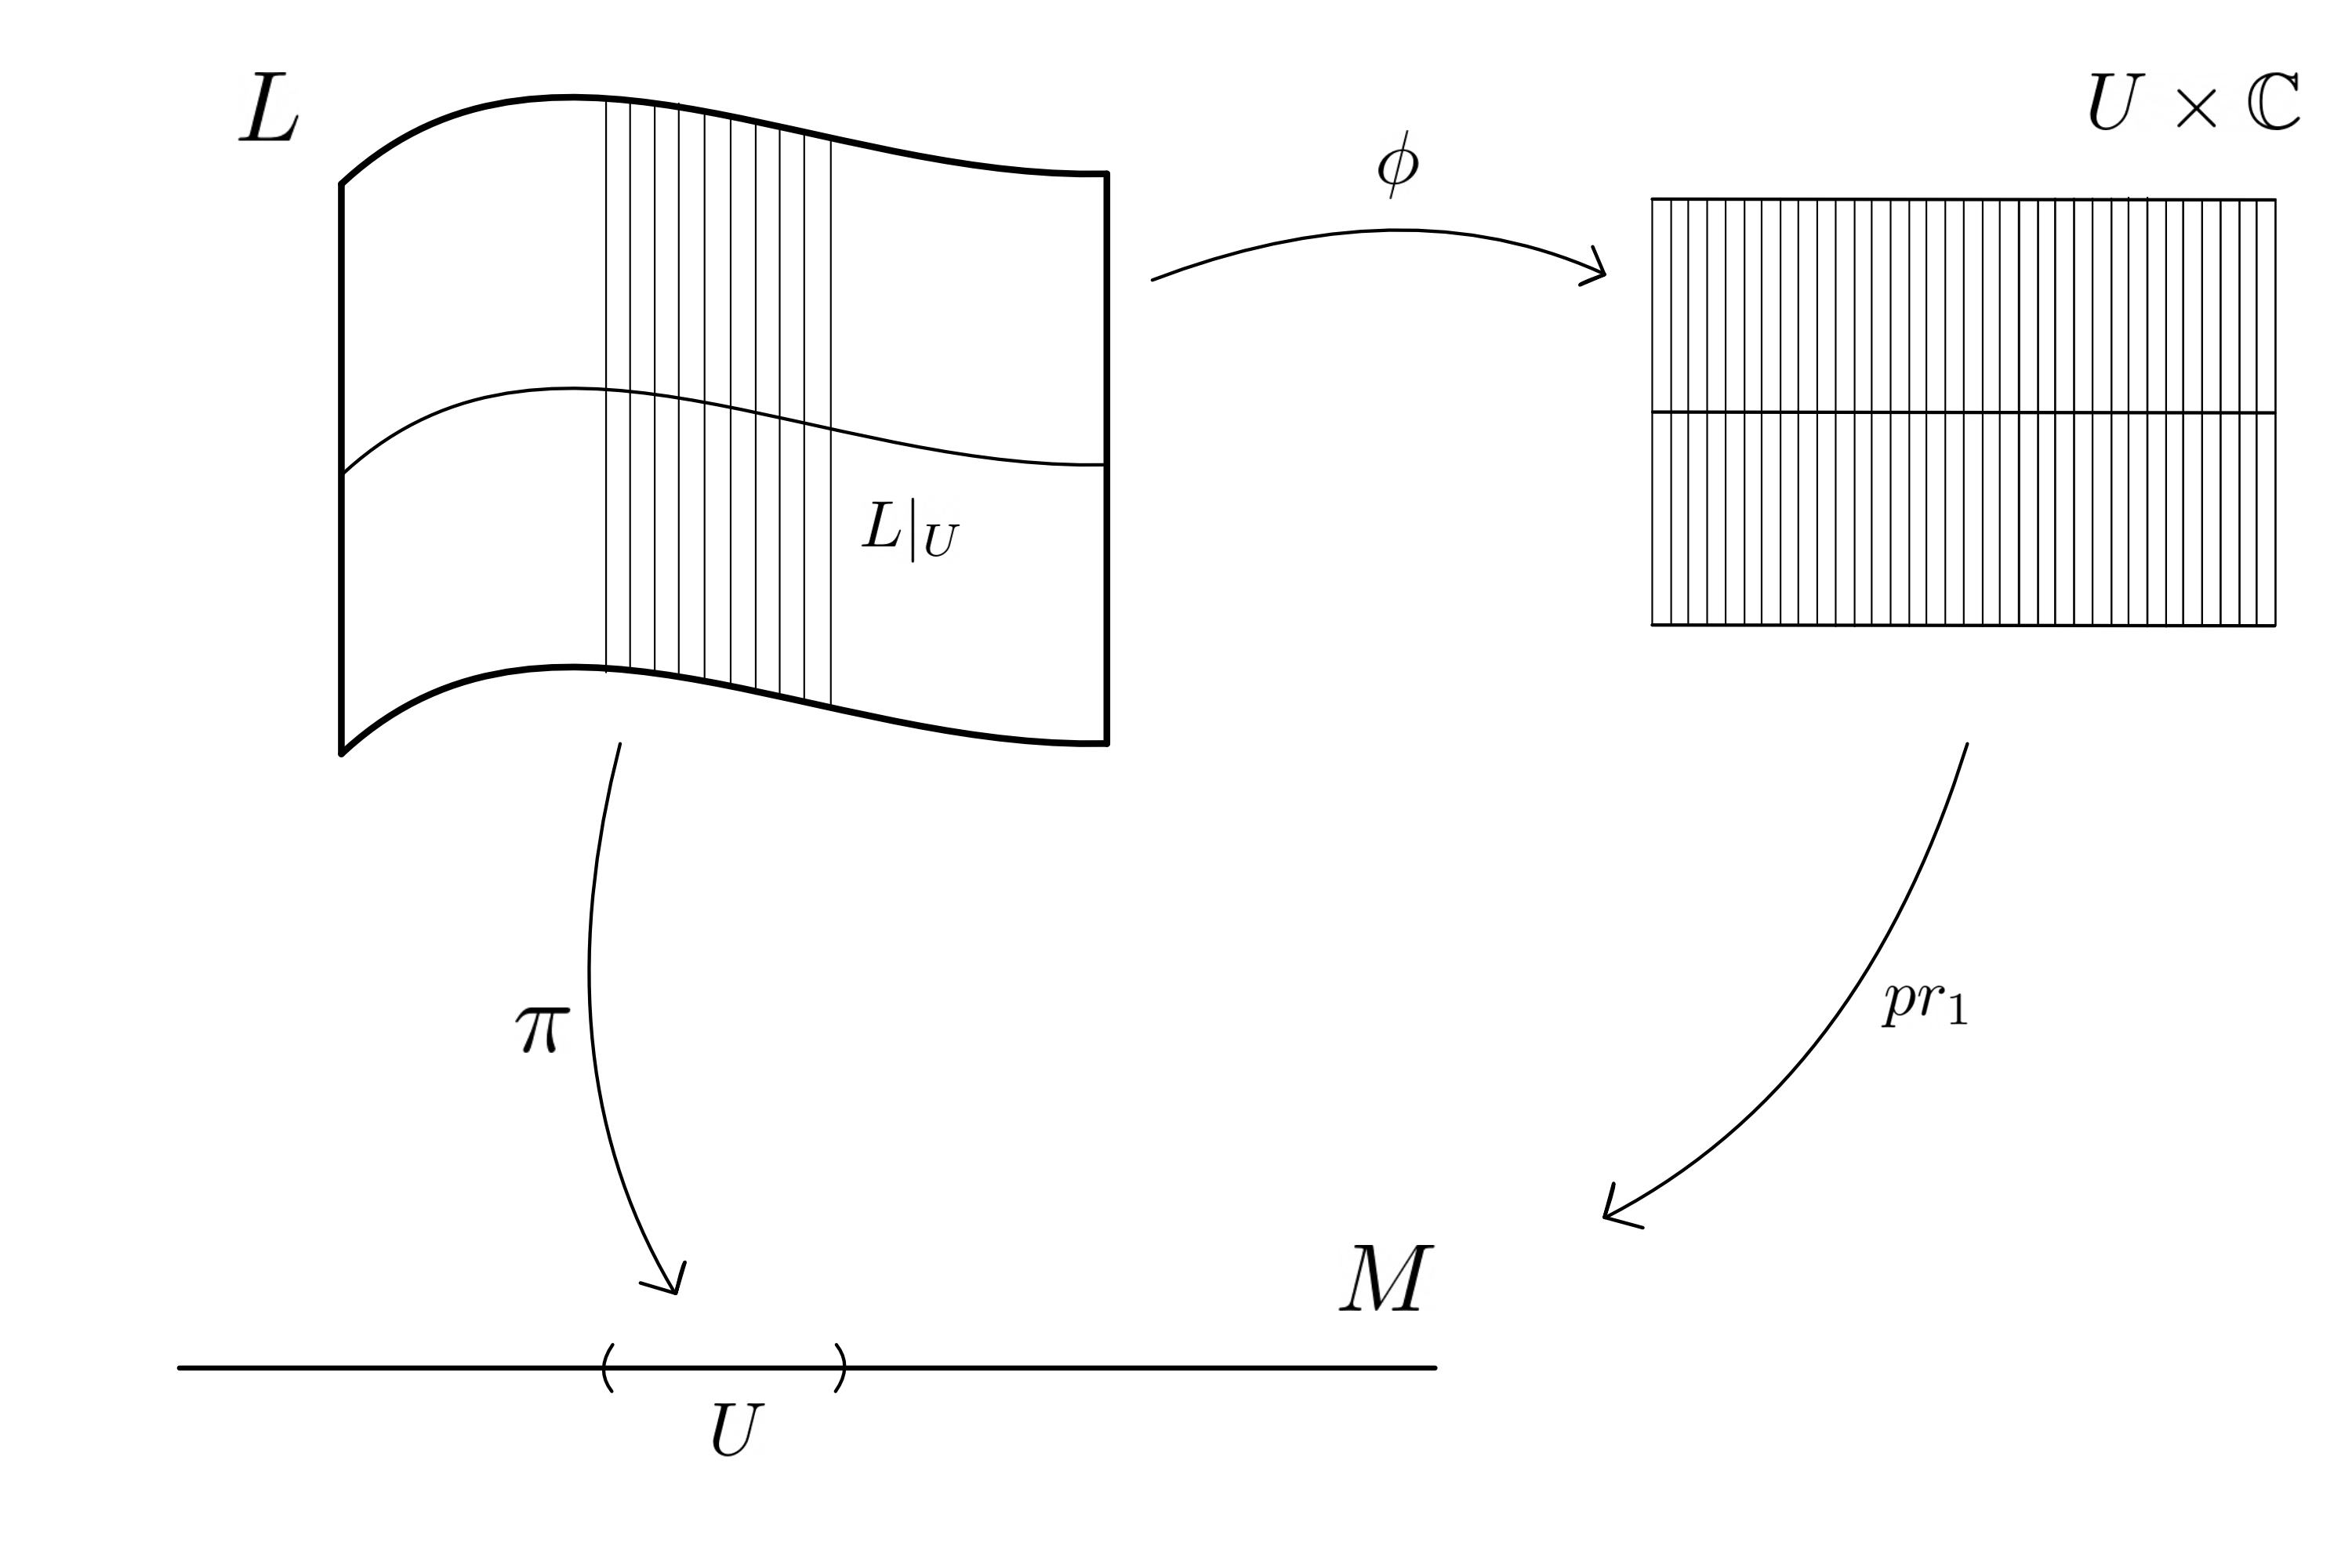
\includegraphics[width=0.7\linewidth]{Imagenes/definicion de haz}
			\caption{Una trivialización de un haz lineal.}
			\label{fig:definicion-de-haz}
		\end{figure}
		
	\end{itemize}
    \end{definition}

    \begin{remark}
    	Sea $ (L,\pi, M) $ es un haz lineal holomorfo. Al espacio $M$ se le llama \textbf{espacio base}, al espacio $ L $ se le llama \textbf{espacio total} y a la función sobreyectiva $\pi:L\to M$ se le llama \textbf{proyección}. Cuando la proyección es clara, se suele denotar $ L\longrightarrow M$ o
    	\begin{center}
    		\begin{tikzcd}
    			L \\
    			\\
    			M
    			\arrow[no head, from=1-1, to=3-1]
    		\end{tikzcd}
    	\end{center}
    	Y si el espacio base también es claro o es fijo, solo decimos que $L$ es un haz lineal. 
    \end{remark}

    \begin{example}[Haz trivial]\label{haztrivial}
    	Sea $M$ un espacio topológico. Notemos que el espacio producto $L:=M\times\cc$ tiene una función proyección a la primera entrada
    	\begin{align*}
    		\pi:&M\times\cc\longrightarrow M\\
    		&(p,z)\mapsto p
    	\end{align*}
    	la cual es holomorfa y sobreyectiva. Si $p\in M$, entonces
    	\begin{align*}
    		L_p=\pi^{-1}(p)=\{p\}\times\cc\cong \cc.
    	\end{align*}
    	Luego, para toda cubierta $\{U_i\}_{i\in I}$ de $M$, tenemos que 
    	\begin{align*}
    		L|_{U_i}=\pi^{-1}(U_i)=U_i\times \cc.
    	\end{align*} 
    	Así, la trivialización local está dada por $\{U_i\}_{i\in I}$ y los biholomorfismos identidad $id_i:L|_{U_i}\to U_i\times\cc$ y claramente conmuta el diagrama
    	\begin{center}
    		\begin{tikzcd}
    			{L|_{U_i}:=\pi^{-1}(U_i)} && {U_i\times\cc} \\
    			\\
    			& M
    			\arrow["{id_i}", from=1-1, to=1-3]
    			\arrow["\pi"', from=1-1, to=3-2]
    			\arrow["{\pi_1}", from=1-3, to=3-2]
    		\end{tikzcd}
    	\end{center}
    	Por lo tanto, $(M\times\cc,\pi_1,M)$ es un haz lineal sobre $M$. 
    \end{example}
    
    Sea $L$ un haz lineal sobre la variedad compleja $M$. Tomemos una trivialización $\{U_i\}_{i\in I}$ de $L$. Es decir, para cada $i$ existe un biholomorfismo
    \begin{equation*}
    	\psi_i :L|_{U_i}\longrightarrow U_i\times \mathbb{C}
    \end{equation*}
    En una intersección $U_{ij}:=U_i\cap U_j$, ambas trivializaciones difieren por multiplicación por una función holomorfa no nula
    \begin{equation*}
    	\psi_i\circ \psi_j^{-1}(x,z)=(x,g_{ij}(x)z),
    	\qquad x\in U_i\cap U_j,
    \end{equation*}
    donde
    \begin{equation*}
    	g_{ij}\in \mathcal{O}^*(U_i\cap U_j).
    \end{equation*}
    
    \begin{figure}[H]
    	\centering
    	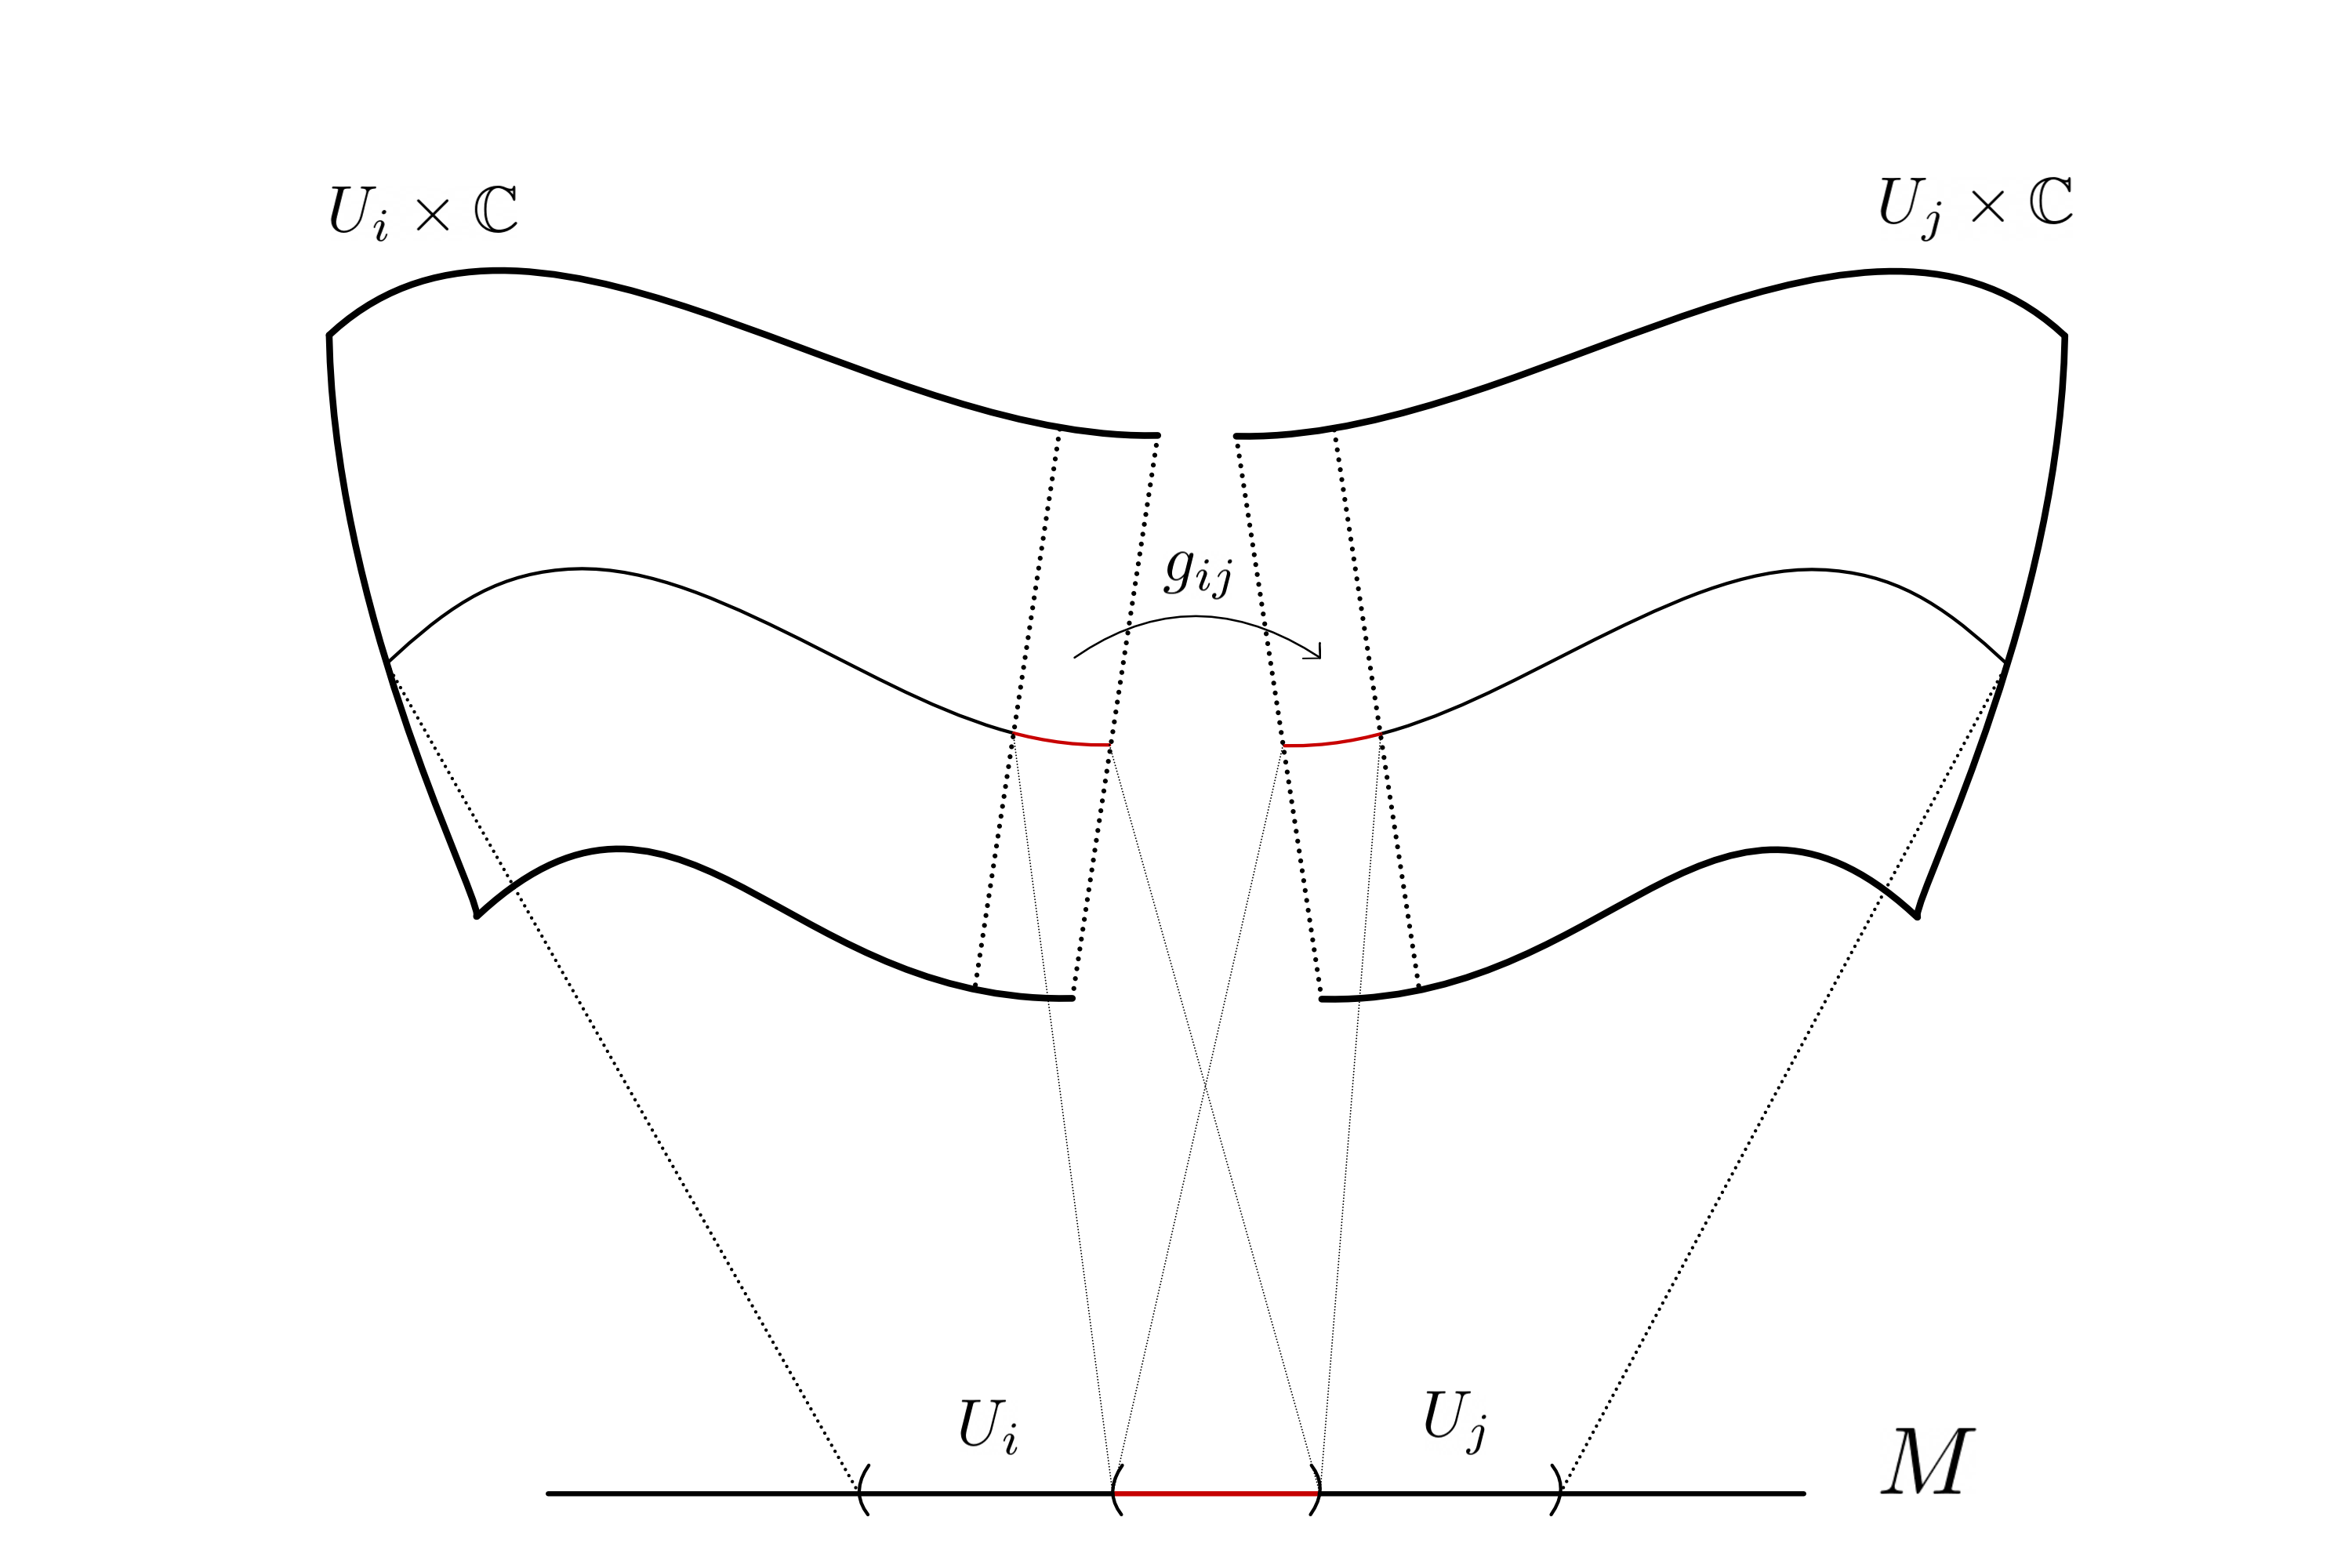
\includegraphics[width=0.5\linewidth]{Imagenes/funciones de transición}
    	\caption{Representación de las funciones de transición}
    	\label{fig:funciones-de-transicion}
    \end{figure}
    
    \begin{remark}\label{cociclos}
    	A las funciones $g_{ij}$ se le llaman \textbf{funciones de transición} y cumplen dos propiedades
    	\begin{align*}
    		g_{ii}&=1,\qquad \text{en }\enspace U_i;\\
    		g_{ij}g_{jk}g_{ki}&=1,\qquad \text{en }\enspace U_i\cap U_j\cap U_k.
    	\end{align*}
    	llamadas \textbf{condiciones de cociclo}.
    \end{remark}

	\begin{example}\label{gijhaztrivial}
		Consideremos el haz trivial $L=M\times \cc$. Por el ejemplo \ref{haztrivial}, sabemos que para cualquier cubierta $\{U_i\}_{i\in I}$ de $M$ se tiene la trivialización
		\begin{align*}
			\psi_i=L|_{U_i}\longrightarrow U_i\times \cc\\
			(p,z)\mapsto (p,z).
		\end{align*}
		Por lo tanto, las funciones de transición de $L$ están dadas por
		\begin{equation*}
			g_{ij}=1,\qquad \text{para todo }i,j\in I.
		\end{equation*}
	\end{example}
	
	Las funciones de transición contienen toda la información necesaria para reconstruir el haz lineal. De hecho, dos haces son isomorfos si y solo si sus funciones de transición representan el mismo cociclo, y recíprocamente, toda colección de funciones que satisfaga las condiciones de cociclo determina un haz lineal.
    
    \begin{propo}[Construcción de un haz holomorfo]\parencite[Chap. 3, Sec. 1, Prop. 3.5]{leecomplex}
	   Sea $M$ una variedad compleja y $\{U_i\}_{i\in I}$ una cubierta de $M$. Supongamos que para cada $i$ y $j$ tal que $ U_{ij} \neq \emptyset$ tenemos una función holomorfa $g_{ij}:U_{ij}\to \cc^*$ tales que satisfacen las condiciones de cociclos, entonces existe un haz lineal holomorfo $ L\longrightarrow M $ que admite una trivialización en $\{U_i\}_{i\in I}$ y con funciones de transición $g_{ij}$.
    \end{propo}

\subsection{Operaciones con haces lineales}

	De la proposición anterior se sigue que, para construir un haz lineal, basta definir funciones de transición que satisfagan la condición de cociclo. Esta observación proporciona un método natural para obtener nuevos haces lineales a partir de otros ya dados mediante sus funciones de transición.

\begin{definition}
	Sean $L$ y $L'$ dos haces lineales sobre $M$, con funciones de transición $\{U_i,g_{ij}\}$ y $\{U'_i,g'_{ij}\}$, respectivamente.
	\begin{enumerate}
		\item Definimos el \textbf{haz dual} de $L$, denotado por $L^*$, como el haz lineal cuyas funciones de transición son
		\begin{equation*}
			g_{ij}^{-1}:=\frac{1}{g_{ij}}.
		\end{equation*}
		\item Definimos el \textbf{producto tensorial} $L\otimes L'$ como el haz lineal cuyas funciones de transición son
		\begin{equation*}
			g_{ij}g'_{ij},
		\end{equation*}
		en las intersecciones donde ambas estén definidas\footnote{Las funciones de transición no tienen por qué estar definidas sobre los mismos abiertos. En tal caso, se considera un refinamiento común de las cubiertas, obtenido al intersectar los abiertos de ambas cubiertas.}.
		
		\item Para $k\in \mathbb{N}$, se denota
		\begin{equation*}
			L^{k}:=\underbrace{L\otimes\cdots\otimes L}_{k\text{ veces}},
		\end{equation*}
		al $k$-ésimo producto tensorial de $L$ consigo mismo. Además, usamos la notación 
		\begin{equation*}
			L^{-k}:=(L^*)^k
		\end{equation*}
	\end{enumerate}
\end{definition}	

	
	
	\begin{example}\label{Ltensordual}
		Sea $L$ un haz lineal sobre $M$ con funciones de transición $\{U_i,g_{ij}\}$ de $M$, entonces las funciones de transición de $L\otimes L^*$ están dadas por
		\begin{equation*}
			g_{ij}g_{ij}^{-1}=1,\qquad\text{para todo }i,j\in I.
		\end{equation*}
		Por el ejemplo \ref{gijhaztrivial}, el haz lineal $L\otimes L^*$ corresponde con el haz trivial de $M$.
	\end{example}
	
	\begin{definition}
		Sea $f:N\to M$ una aplicación holomorfa y $\pi:L\to M$ un haz lineal sobre $M$. El \textbf{pullback} de $L$ a través de $f$ es el espacio 
		\begin{equation*}
			f^*L=\{(n,l)\in N\times L: f(n)=\pi(l)\}.
		\end{equation*}
		junto a las aplicaciones naturales
		\begin{align*}
			\pi':f^*L\longrightarrow N\\
			(n,l)\mapsto n
		\end{align*}
		\begin{align*}
			h:f^*L\longrightarrow L\\
			(n,l)\mapsto l
		\end{align*}
		de forma que el siguiente diagrama conmuta
		\begin{center}
			\begin{tikzcd}
				{f ^*L} && L \\
				\\
				N && M
				\arrow["{h}", from=1-1, to=1-3]
				\arrow["{\pi'}"', from=1-1, to=3-1]
				\arrow["\pi", from=1-3, to=3-3]
				\arrow["f"', from=3-1, to=3-3]
			\end{tikzcd}
		\end{center}
	\end{definition}
	
	\begin{remark}
		Si $\{U_i\}_{i\in I}$ es una cubierta de $M$ sobre la cual $L$ se trivializa, con funciones de transición
		\begin{equation*}
				g_{ij}\in \mathcal{O}^*(U_i\cap U_j),
		\end{equation*}
		entonces el pullback $f^*L\to N$ se trivializa sobre la cubierta inducida $\{f^{-1}(U_i)\}_{i\in I}$ de $N$.
		
		En efecto, sobre cada $f^{-1}(U_i)$ definimos la trivialización local de $ f^*L$ usando la trivialización de $L$ sobre $U_i$. Si
		\begin{equation}
			\psi_i:\pi^{-1}(U_i)\longrightarrow U_i\times \mathbb{C}
		\end{equation}
		es una trivialización de $L$, entonces se obtiene una trivialización de $f^*L $ sobre $f^{-1}(U_i) $ dada por
		\begin{align*}
			\widetilde{\psi}_i:f^*L|_{f^{-1}(U_i)}&\longrightarrow f^{-1}(U_i)\times \mathbb{C}\\
			(n,\ell)&\mapsto \bigl(n, z\bigr),
		\end{align*}
		donde $\psi_i(\ell)=(f(n),z)$. Ahora, en una intersección $f^{-1}(U_{ij})$, el cambio de trivialización viene dado por
		\begin{equation*}
			\widetilde{\psi}_i\circ \widetilde{\psi}_j^{-1}(n,z)=\bigl(n, (g_{ij}\circ f)(n) z\bigr).
		\end{equation*}
		Por tanto, las funciones de transición del pullback $f^*L$ son precisamente
		\begin{equation*}
			(f^*g)_{ij}=g_{ij}\circ f
			\quad\text{en}\quad
			f^{-1}(U_{ij}).
		\end{equation*}
	\end{remark}

\subsection{Espacio de secciones}

	\begin{definition}
		Sea $\pi:L\to M$ un haz lineal sobre una variedad compleja $M$. Una \textbf{sección} (global) de $L$ es una aplicación holomorfa $s:M\to L$ tal que
		\begin{equation*}
			\pi\circ s=\mathrm{id}_M.
		\end{equation*}
		Una \textbf{sección local} es una sección $s:U\to L$ definida solo en un abierto $U\subset M$. 
		\begin{figure}[H]
			\centering
			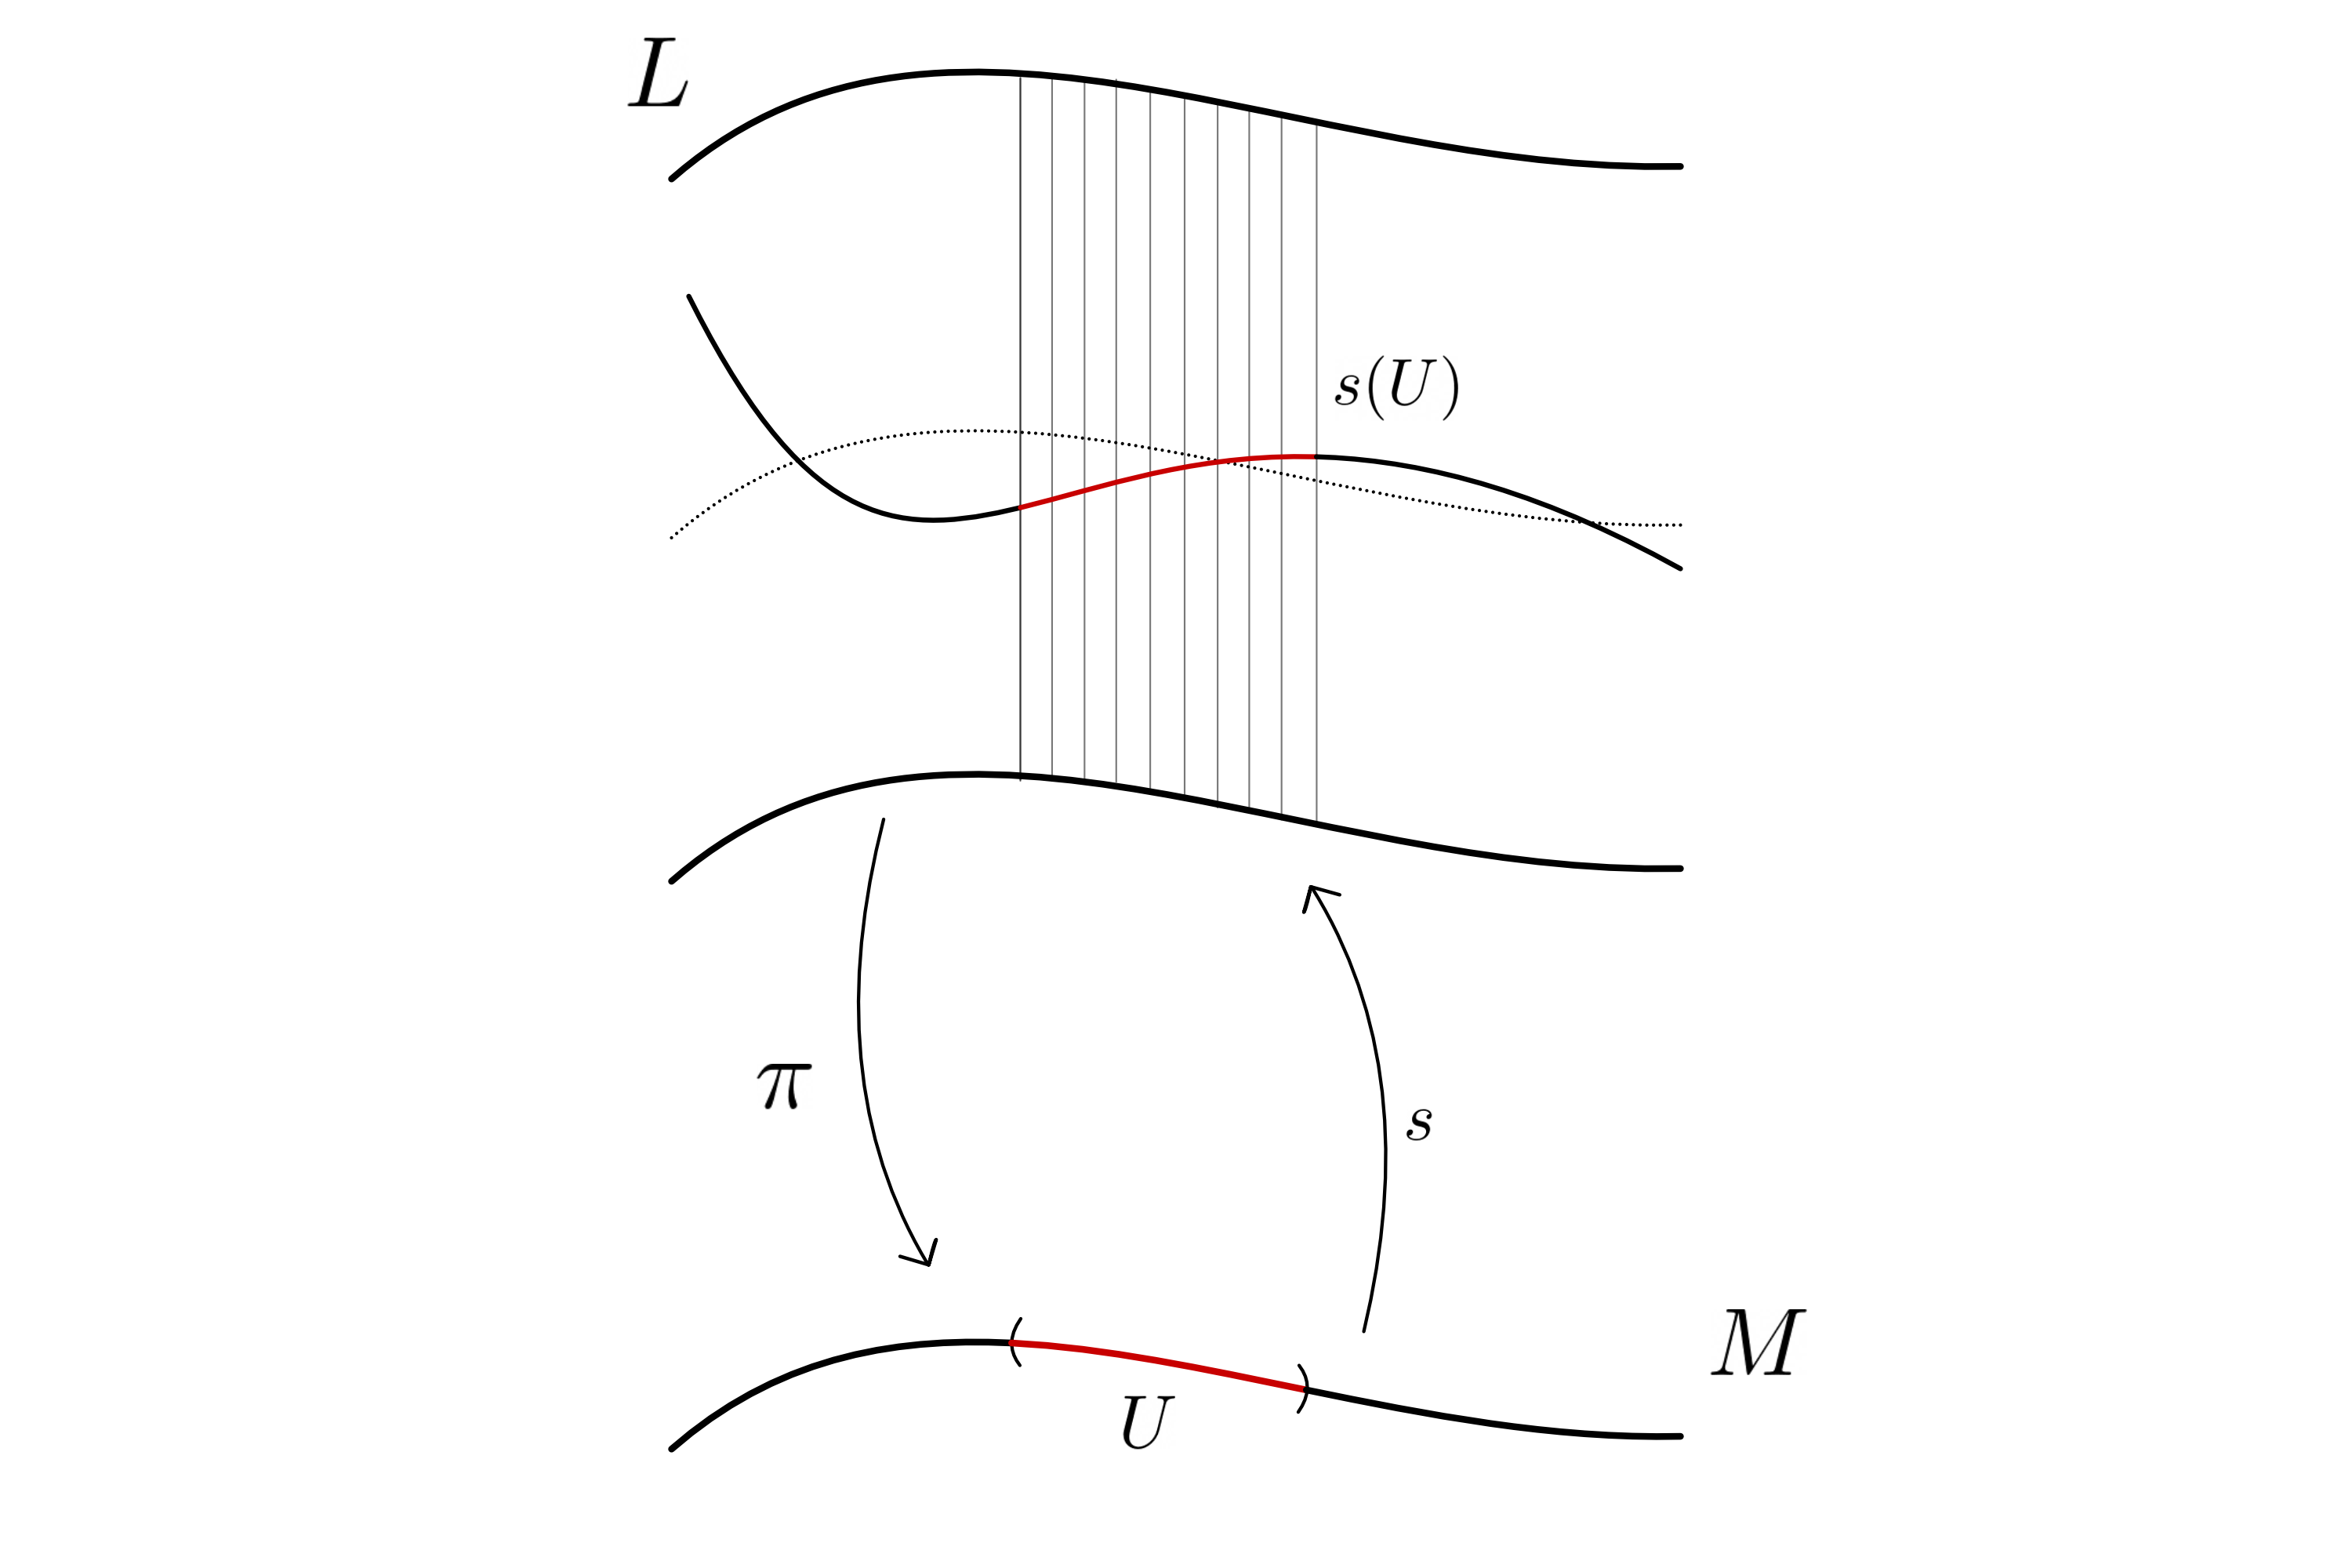
\includegraphics[width=0.5\linewidth]{Imagenes/seccion local}
			\caption{Interpretación de las secciones locales}
			\label{fig:seccion-local}
		\end{figure}
		
	\end{definition}
	
	Si $p\in M$ y $s:M\to L$ es una sección global, entonces $\pi(s(p))=p$. Así, $s(p)\in \pi^{-1}(p)=L_p$. Esto significa que las secciones $s$ siempre mandan a los puntos $p\in M$ a sus fibras $L_p$. Entonces, podemos pensar que una sección encaja a $M$ dentro de $L$ de manera que intersecta solo una vez a cada fibra. En particular, existe siempre una sección $s_0:M\to L$ definida como
	\begin{equation*}
		s_0(p)=0\in L_p,\qquad \text{para todo }p\in M.
	\end{equation*}
	La sección $s_0$ es llamada \textbf{sección cero} de $L$.
	
	\begin{definition}
		Sea $M$ una variedad compleja y $\pi:L\to M$ un haz lineal. Definimos el \textbf{espacio de secciones holomorfas} como
		\begin{equation*}
			\oo(U;L):=\{s:U\to L: s\text{ es una sección local de }L\}.
		\end{equation*}
	\end{definition}
	
	\begin{remark}\label{seccionlocalholomorfa}
		Sea $\pi:L\to M$ un haz lineal y $s:U\to L$ una sección local. Por definición
		\begin{equation}\label{pis(p)}
			\pi \circ s(p)=p,\qquad p\in U.
		\end{equation} 
		Supongamos que $L$ se trivializa en $U$, entonces
		\begin{equation*}
			\psi:\pi^{-1}(U)\cong U\times \cc.
		\end{equation*}
		Como $s(p)$ pertenece a la fibra de $p$, tenemos que
		\begin{equation*}
			s(p)\in \pi^{-1}(U)\cong U\times \cc.
		\end{equation*}
		Por (\ref{pis(p)}), tenemos que $s$ conmuta con la proyección a la primera entrada. Por lo que
		\begin{equation*}
			\psi(s(p))=(p,z)\in U\times \cc.
		\end{equation*}
		Como $s$ es holomorfa, existe una función holomorfa $f\in \oo_M(U)$ tal que
		\begin{equation*}
			\psi(s(p))=(p,f(p)).
		\end{equation*}
		Más aún, consideremos una intersección de abiertos trivializantes $U_i\cap U_j$ con funciones de transición $g_{ij}$. Entonces
		\begin{equation*}
			\psi_i(s(p))=(p,f_i(p)),\qquad \psi_j(s(p))=(p,f_j(p)).
		\end{equation*}
		Por definición de las funciones de transición
		\begin{equation*}
			\psi_i\circ \psi_j^{-1}(p,z)=(p,g_{ij}(p)z).
		\end{equation*}
		De esta manera,
		\begin{equation*}
			(p,f_i(p))=\psi_i(s(p))=\psi_i(\psi_j^{-1}(p,f_j(p)))=(p,g_{ij}(p)f_j(p)).
		\end{equation*}
		Por lo tanto, 
		\begin{equation*}
			f_i(p)=g_{ij}(p)f_j(p).
		\end{equation*}
	\end{remark}
	
	Notemos que las secciones holomorfas de un haz lineal pueden sumarse y multiplicarse por escalares complejos, gracias a la estructura de $\cc$-espacio vectorial de las fibras. Además, por la observación anterior, estas operaciones preservan la holomorfía, pues se reducen punto a punto a operaciones entre funciones holomorfas. En consecuencia, tenemos lo siguiente:
	
	\begin{propo}
		Sea $M$ una variedad compleja y $\pi:L\to M$ un haz lineal. Entonces el funtor definido por
		\begin{align*}
			\mathcal{O}(L)(U):=\mathcal{O}(U;L)
		\end{align*}
		para todo abierto $U$ de $M$, es una gavilla de $\cc$-espacios vectoriales.
	\end{propo}
	
	La demostración de esta proposición es análoga a la de la gavilla de funciones holomorfas. Además, las secciones holomorfas pueden multiplicarse por funciones holomorfas locales y el resultado sigue siendo una sección holomorfa. Esto muestra que la gavilla $\mathcal{O}(L)(\_)$ posee de manera natural una estructura de gavilla de $\mathcal{O}_M$-módulos. En particular, por la observación \ref{seccionlocalholomorfa}, dicha gavilla es localmente isomorfa a $\mathcal{O}_M$; es decir, $\mathcal{O}(L)(\_)$ es una gavilla de $\mathcal{O}_M$-módulos localmente libre de rango $1$. Por lo tanto, $\mathcal{O}(L)(\_)$ es una gavilla coherente (véase \parencite[Chap.~5, Sec.~3.4]{griffiths}).

	\begin{example}\label{seccionesdeltrivial}
		Consideremos el haz trivial $L$ sobre $M$ y tomemos $U$ un abierto no vacío de $M$. Entonces
		\begin{equation*}
			\pi^{-1}(U)= U\times \cc.
		\end{equation*}
		Por la observación \ref{seccionlocalholomorfa}, tenemos que si $s$ es una sección local sobre $U$ entonces
		\begin{equation*}
			s(p)=(p,f(p)),\qquad \text{para todo }\ p\in U,
		\end{equation*}
		donde $f\in\oo_M(U)$. De esta manera, $s$ está totalmente determinada por la función holomorfa $f$. Asimismo, toda función holomorfa $f$ de $M$ determina una sección local de $L$. Por lo tanto, la gavilla $\mathcal{O}(L)$ corresponde con la gavilla de funciones holomorfas $\oo_M$.
	\end{example}
	
	\begin{theorem}
		Sea $M$ una variedad compleja compacta y $\pi:L\to M$ un haz lineal. Entonces el espacio de secciones globales $	H^0(M,L):=\mathcal{O}(M;L)$ \footnote{La notación proviene del hecho de que el espacio de secciones globales coincide con el grupo de cohomología de Čech de grado $0$ de la gavilla asociada al haz lineal $L$.} es un $\cc$-espacio vectorial de dimensión finita.
	\end{theorem}
	
	Este resultado muestra nuevamente la rigidez de la geometría compleja, pues aunque un haz lineal pueda admitir muchas secciones locales, la compacidad de la variedad impone una fuerte restricción sobre las secciones holomorfas globales. En general, la finitud de $H^0(M,L)$ se deduce del hecho de que la gavilla $\mathcal{O}(L)(\_)$ es coherente (véase \parencite[Chap.~VIII, Sec.~A, Cor.~10]{gunningrossi}). Sin embargo, también puede obtenerse mediante argumentos analíticos más elementales, introduciendo una norma global sobre $\mathcal{O}(M;L)$ y demostrando que la bola unitaria cerrada es compacta (véase \parencite[Chap.~3, Sec.~1, Theo.~3.13]{leecomplex}).
	
	\begin{example}\label{H0deltrivial}
		Consideremos el haz trivial $L$ sobre $M$. Por el ejemplo \ref{seccionesdeltrivial} tenemos que
		\begin{equation*}
			H^0(M,L)\cong \oo_M(M).
		\end{equation*} 
		Si $M$ es compacta, toda función holomorfa global es constante (véase teorema \ref{holomorfasglobal}), luego
		\begin{equation*}
			H^0(M,L)\cong\cc.
		\end{equation*}
		Por lo tanto,
		\begin{equation*}
			\dim_\cc H^0(M,L)=1.
		\end{equation*}
	\end{example}
	
	\begin{example}[Secciones del pullback]\label{seccionespullback}
		Sea $f:N\to M$ una aplicación holomorfa y $\pi:L\to M$ un haz lineal. Recordemos que el pullback está dado por
		\begin{equation*}
			f^*L=\{(n,l)\in N\times L:f(n)=\pi(l)\}.
		\end{equation*}
		Sea $s\in H^0(M,L)$ una sección global de $L$. Definamos
		\begin{align*}
			f^*s&:N\longrightarrow f^*L\\
			f^*s(n)&=(n,s(f(n))).
		\end{align*}	
		Es inmediato que $f^*s$ es holomorfa y 
		\begin{equation*}
			(\pi'\circ f^*s)(n)=\pi'(f^*s(n))=\pi'(n,s(f(n)))=n.
		\end{equation*}
		De esta manera, $f^*s$ es una sección global de $f^*L$. Notemos además que esta construcción determina una aplicación $\cc$-lineal
		\begin{equation*}
			f^*:H^0(M,L)\longrightarrow H^0(N,f^*L).
		\end{equation*}
		En general, $f^*$ no es sobreyectiva. Por ejemplo, tomemos $M=\{\mathrm{pt}\}$ y $L=\cc$ es haz trivial sobre $M$. Entonces $H^0(M,L)\cong\cc$, mientras que para cualquier variedad compleja $N$ se tiene que
		\begin{equation*}
			H^0(N,f^*L)\cong H^0(N,N\times \cc)=\oo_N(N).
		\end{equation*} 
		Tomando $N=\cc$, entonces $\oo_N(N)$ tiene dimensión infinita pues $N$ no es compacta. Por lo que $f^*$ determina un morfismo lineal
		\begin{equation*}
			\cc\longrightarrow \oo(\cc).
		\end{equation*}
		el cual no es sobreyectivo.
	\end{example}
	
\section{Haces amplios y encajes}

Los haces lineales son importantes en el estudio de los encajes al espacio proyectivo porque actúan como el mecanismo que nos permite construir aplicaciones holomorfas desde una variedad compleja hacia $\pp^N$. Sin la estructura de los haces lineales, no existiría una forma natural de generar las coordenadas homogéneas necesarias para \enquote{sumergir} una variedad compleja en el mundo algebraico del espacio proyectivo. 

\subsection{Haces lineales del espacio proyectivo}

	Consideremos el espacio proyectivo $\pp^n$ y definamos el conjunto
	\begin{equation*}
		\mathcal{O}(-1)=\{(l,z)\in\pp^n\times \cc^{n+1}:l\in\pp^n, z\in l\text{ ó }z=0\}.
	\end{equation*}
	Notemos que la proyección a la primera entrada $\pi:\mathcal{O}(-1)\to\pp^n$ es una aplicación holomorfa sobreyectiva. Con esto podemos ver que:
	
	\begin{propo}
		$\mathcal{O}(-1)$ es un haz lineal del espacio proyectivo $\pp^n$.
	\end{propo}
	\begin{proof}
		Sea $l\in\pp^n$, entonces la fibra $\pi^{-1}(l)$ es el conjunto de puntos $z\in\cc^{n+1}$ que pertencen a la línea compleja $l$. Con lo cual,
		\begin{equation*}
			\pi^{-1}(l)\cong \cc.
		\end{equation*}
		Consideremos $\pp^n=\bigcup_{i=0}^n U_i$ la cubierta estandar afin del espacio proyectivo. 
%		Una trivialización canónica de $\oo(-1)$ sobre la cubierta es
%		\begin{align*}
%			\psi_i:\pi^{-1}(U_i)\longrightarrow U_i\times\cc\\
%			(l,z)\mapsto (l,\mathrm{pr}_i(z))
%		\end{align*}
%		donde $z=(z_0,\dots,z_n)$. 
		
		Determinemos sus funciones de transición a partir de trivializaciones locales. Para cada abierto $U_i$, definimos
		\begin{equation*}
			\psi_i:\pi^{-1}(U_i)\longrightarrow U_i\times \cc
		\end{equation*}
		mediante
		\begin{equation*}
			\psi_i(l,w)=
			\left(
			l,
			\frac{w_i}{z_i}
			\right),
		\end{equation*}
		donde $w=(w_0,\dots,w_n)\in l$. Esta expresión está bien definida, pues como $w$ pertenece a la recta $l$, existe $\lambda\in\cc$ tal que $w=\lambda z$, y por tanto
		\begin{equation*}
			\frac{w_i}{z_i}=\lambda.
		\end{equation*}
		La inversa de $\psi_i$ está dada por
		\begin{equation*}
			\psi_i^{-1}([z],\lambda)=([z],\lambda z),
		\end{equation*}
		de modo que $\psi_i$ es una trivialización holomorfa.
		
		Ahora, sobre la intersección $U_i\cap U_j$, el cambio de trivialización
		\begin{equation*}
			\psi_i\circ \psi_j^{-1}:
			(U_i\cap U_j)\times\cc
			\longrightarrow
			(U_i\cap U_j)\times\cc,
		\end{equation*}
		está dado por
		\begin{equation*}
			\psi_i\circ \psi_j^{-1}([z],\lambda)
			=\left([z],\frac{z_j}{z_i}\lambda \right).
		\end{equation*}
		Por lo tanto, las funciones de transición de $\mathcal{O}(-1)$ son
		\begin{equation*}
			g_{ij}=\frac{z_j}{z_i}.
		\end{equation*}
	\end{proof}
	
	\begin{figure}
		\centering
		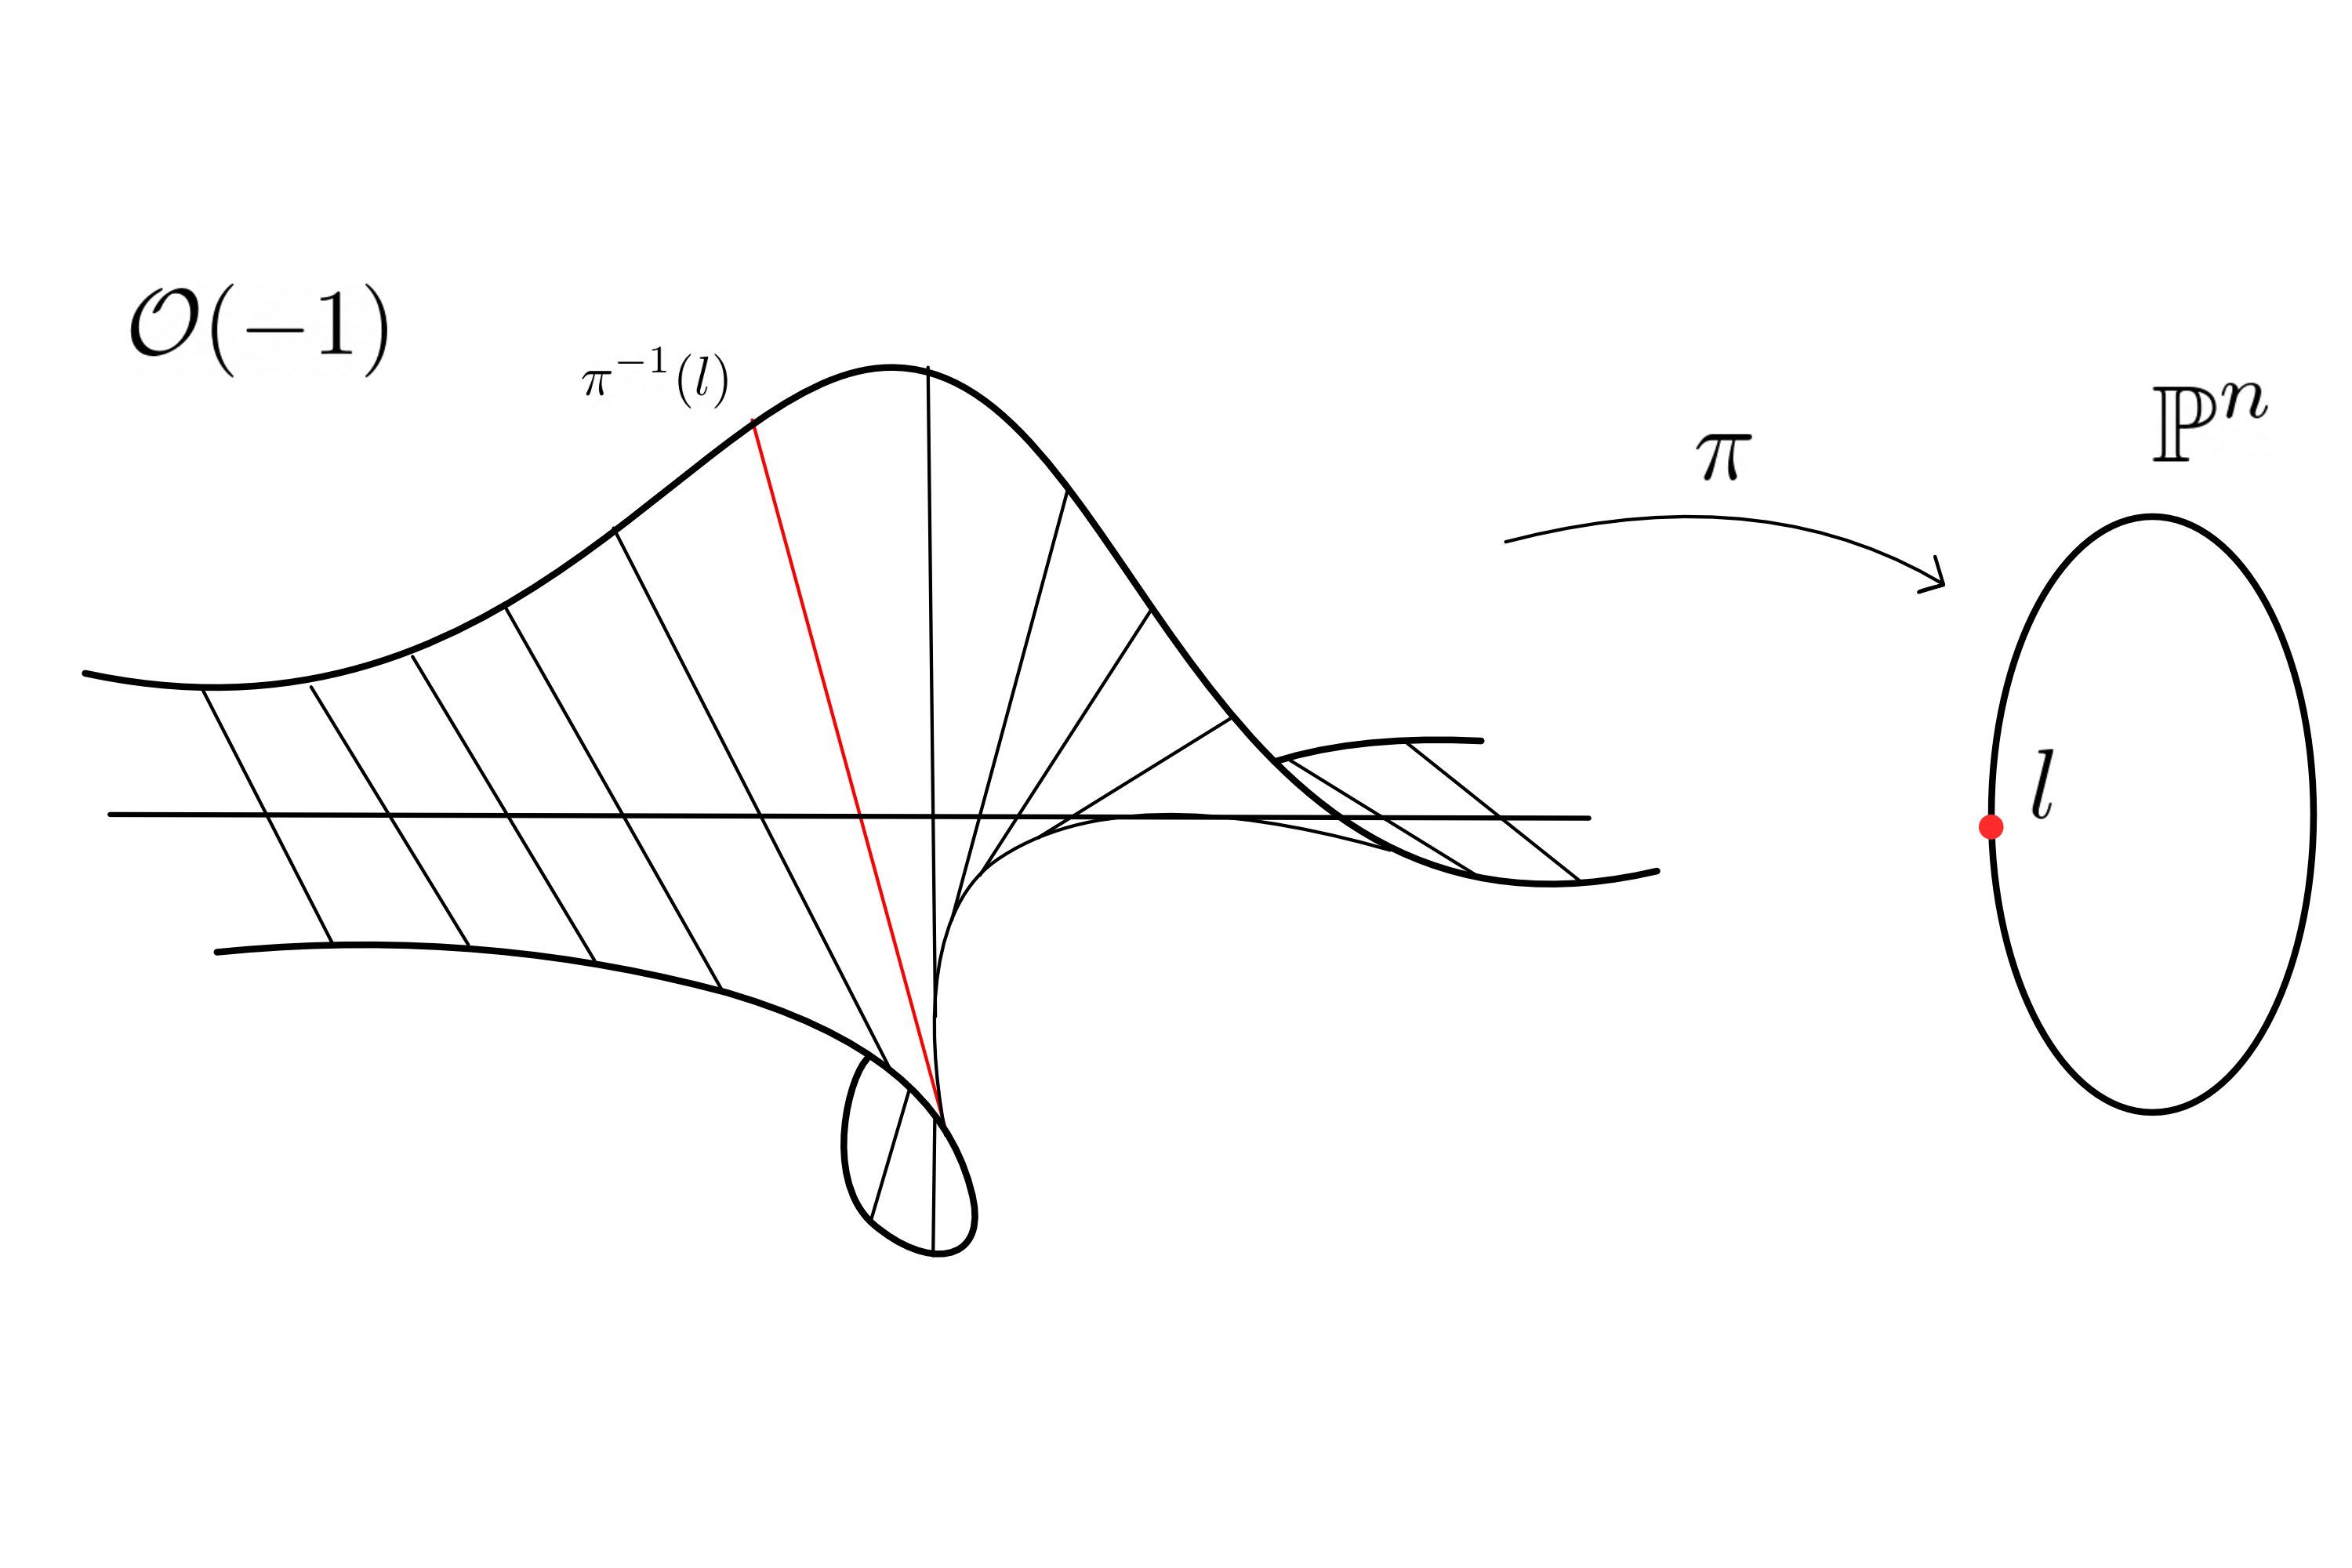
\includegraphics[width=0.7\linewidth]{Imagenes/tautologico}
		\caption{Interpretación geométrica del haz lineal $\mathcal{O}(-1)$.}
		\label{fig:tautologico}
	\end{figure}
	
	
	\begin{definition}
		Consideremos el haz lineal $\oo(-1)$ sobre el espacio proyectivo $\pp^n$.
		\begin{enumerate}
			\item El haz lineal $\mathcal{O}(-1)$ es llamado \textbf{haz tautológico}.
			\item El haz dual $\mathcal{O}(1):=\mathcal{O}(-1)^*$ es llamado \textbf{haz de hiperplanos}.
			\item El haz trivial sobre $\pp^n$ lo denotamos como $\mathcal{O}(0):=\pp^n\times\cc$.
			\item La potencia tensorial la denotamos como $\mathcal{O}(-d):=\mathcal{O}(-1)^d$ y  $\mathcal{O}(d):=\mathcal{O}(1)^{d}$.
		\end{enumerate}
	\end{definition}

	\begin{lemma}\label{seccionesnotriviales}
		Sea $L$ un haz lineal holomorfo sobre una variedad compleja conexa compacta $M$. Entonces $L$ es trivial si, y solo si, $L$ y su dual $L^*$ admite secciones globales no triviales.  
	\end{lemma}
	\begin{proof}
		Supongamos que $L$ es trivial. Por el ejemplo \ref{seccionesdeltrivial}, $L$ admite secciones constantes no cero. Además, el dual $L^*$ vuelve a ser $L$, por lo que $L^*$ también admite secciones constantes no cero.
		
		Ahora supongamos que $L$ y $L^*$ admite secciones globales no cero. Tomemos las secciones globales no cero
		\begin{equation*}
			s\in H^0(M,L),
			\qquad
			t\in H^0(M,L^*).
		\end{equation*}
		Entonces por el ejemplo \ref{Ltensordual} tenemos que
		\begin{equation*}
			s\otimes t\in H^0(M,L\otimes L^*)\cong H^0(M,\oo_M).
		\end{equation*}
		Eso significa que $s\otimes t$ corresponde con una función holomorfa global $f\in \oo_M(M)$. Por el teorema \ref{holomorfasglobal}, $s\otimes t$ es constante. 
		
		Como $s$ y $t$ son holomorfas no cero, siempre existe $r\in M$ tal que $s(r)\neq 0$ y $t(r)\neq 0$. Con lo cual $(s\otimes t)(r)\neq 0$. De esta manera, $s\otimes t\neq 0$. En particular, $s(p)\neq 0$ para todo punto $p\in M$.
		
		Ahora bien, una sección global que nunca se anula trivializa globalmente al haz $L$. Definamos
		\begin{align*}
			\Psi:M\times \cc\longrightarrow L,\\
			\Psi(p,\lambda)=\lambda s(p).
		\end{align*}
		Consideremos una trivialización local $(U,\psi)$ de $L$, entonces
		\begin{equation*}
			s|_U(p)=(p,f(p)),\qquad \text{para todo }\ p\in U
		\end{equation*}
		donde $f\in\oo_M(U)$. Como $s$ nunca se anula, entonces $f$ tampoco nunca se anula. Además, como $L|_U=\pi^{-1}(U)\cong U\times \cc$, entonces a todo punto $x\in L|_U$ se le asocia de manera única un punto $(q,\lambda')\in U\times \cc$. De esta manera, podemos definir $\Psi^{-1}$ localmente como
		\begin{equation*}
			\Psi|_U^{-1}(x)=\left(q,\frac{\lambda'}{f(q)}\right),
		\end{equation*}
		la cual está bien definida porque $f$ nunca se anula.
		Notemos que en efecto es la inversa, pues
		\begin{align*}
			\Psi\circ\Psi^{-1}(x)=\Psi\left(q,\frac{\lambda'}{f(q)}\right)=\frac{\lambda'}{f(q)}s(q)=\frac{\lambda'}{f(q)}(q,f(q))=\left(q,\frac{\lambda'}{f(q)}f(q)\right)=(q,\lambda')=x,\\
			\Psi^{-1}\circ\Psi(p,\lambda)=\Psi^{-1}(\lambda s(p))=\Psi^{-1}(\lambda(p,f(p)))=\Psi^{-1}(p,\lambda f(p))=\left(p,\frac{\lambda f(p)}{f(p)}\right)=(p,\lambda).
		\end{align*}
		Por lo tanto, $\Psi:M\times \cc\to L$ es un biholomorfismo y $L$ es trivial.
	\end{proof}
	
	Con este lema, podemos probar uno de los resultados más importante de los haces lineales del espacio proyectivo.
	
	\begin{theorem}\label{seccionesproyectivo}
		Consideremos el haz lineal $\oo(1)$ del espacio proyectivo $\pp^n$ y sea $d$ un entero positivo no cero. Entonces se cumple lo siguiente:
		\begin{enumerate}
			\item $H^0(\pp^n, \mathcal{O}(d))\cong \cc[z_0,\cdots,z_n]_{(d)}$
			\item $H^0(\pp^n, \mathcal{O}(0))\cong \cc$
			\item $H^0(\pp^n, \mathcal{O}(-d))\cong\{0\}$
		\end{enumerate}
	\end{theorem}
	\begin{proof} $ $
		\begin{enumerate}
			\item Recordemos que el conjunto $\cc[z_0,\cdots,z_n]_{(d)}$ es el anillo de polinomios homogéneos de grado $d$.
			
			Consideremos la cubierta estandar afín de $\pp^n$
			\begin{equation*}
				\pp^n=\bigcup_{i=0}^n U_i.
			\end{equation*}
			En una intersección $U_j\cap U_k$, las funciones de transición de $\mathcal{O}(-1)$ están dadas por 
			\begin{equation*}
				g_{ij}=\frac{z_j}{z_i}.
			\end{equation*}
			Entonces las funciones de transición de $\mathcal{O}(d)$ son de la forma
			\begin{equation*}
				g'_{ij}=\frac{z_k^d}{z_j^d}.
			\end{equation*}
			Por la observación \ref{seccionlocalholomorfa}, toda sección global $s\in H^0(M,L)$ está determinada por una colección de funciones holomorfas $f_i\in\oo_{\pp^n}(U_i)$ tal que $f_j=\frac{z_k^d}{z_j^d}f_k$ en $U_i\cap U_j$. Consideremos la aplicación cociente
			\begin{align*}
				q:\cc^{n+1}\setminus\{0\}\longrightarrow \pp^n,
			\end{align*}
			entonces el pullback $f'_j=f_j\circ q$ está bien definida y holomorfa cuando $z_j\neq 0$. De la relación
			\begin{equation*}
				z_j^df'_j=z_k^d f'_k
			\end{equation*}
			tenemos que la función
			\begin{equation*}
				F(z):=z_j^df_j([z])
			\end{equation*}
			no depende del índice $j$. Así, $F$ es holomorfa en $\cc^{n+1}\setminus\{0\}$. Por el teorema de Hartog \ref{hartogs}, esta función se extiende holomorfamente a $\cc^{n+1}$. Además, satisface la condición de homogeneidad 
			\begin{equation*}
				F(\lambda z)=(\lambda z_j)^d f_j([\lambda z])=\lambda^d F(z),\qquad \lambda\in\cc^*.
			\end{equation*}
			Al expandir en serie de potencias, esta identidad fuerza que solo aparezcan monomios de grado $d$. 
			Escribiendo
			\begin{equation*}
				F=\sum_\alpha a_\alpha z^\alpha,
			\end{equation*}
			la identidad $ F(\lambda z)=\lambda^dF(z)$ implica que
			\begin{equation*}
				\sum_\alpha a_\alpha \lambda^{|\alpha|}z^\alpha
				=
				\sum_\alpha a_\alpha \lambda^d z^\alpha.
			\end{equation*}
			Por unicidad de la serie de potencias,
			$a_\alpha=0$ si $|\alpha|\neq d$. Con lo cual, $F$ es un polinomio homogéneo de grado $d$.
			
			Consideremos un polinomio $P$ homogéneo de grado $d$, entonces en cada abierto $U_j$ podemos definir
			\begin{equation*}
				f_j([z])=\frac{P(z)}{z_j^d}.
			\end{equation*}
			Esta función es holomofa en $U_j$, y la expresión coincide en las intersecciones pues $P$ es un polinomio homogéneo de grado $d$. Por lo tanto, la colección $\{f_j\}_{j=0}^n$ determina una sección global holomorfa de $\mathcal{O}(d)$.
			
			\item Se sigue del ejemplo \ref{H0deltrivial}.
			
			\item Por el lema \ref{seccionesnotriviales}, tenemos que $\mathcal{O}(-d)=\mathcal{O}(d)^*$ no puede admitir secciones globales no triviales pues el haz $\mathcal{O}(d)$ no es trivial. Por lo que, 
			\begin{equation*}
				H^0(\pp^n,\mathcal{O}(-d))=\{s_0\}\cong \{0\}
			\end{equation*}
			donde $\{0\}$ es el subespacio vectorial de dimensión cero de $\cc$.
		\end{enumerate}
	\end{proof}
	
\subsection{Aplicación asociada a un haz}


    \begin{definition}[Puntos base]
		Sea $L$ un haz lineal sobre una variedad compleja conexa $M$. El conjunto de \textbf{puntos bases} de $L$ está dado por
		\begin{equation*}
			\mathrm{Bs}(L)=\{p\in M:s(p)=0\text{ para todo }s\in H^0(M,L)\},
		\end{equation*}
		donde $s(p)=0$ signifa que la sección $s$ coincide con la sección cero $s_0\in H^0(L,M)$ en el punto $p$.
	\end{definition}

	\begin{remark}
		Sea $L$ un haz lineal sobre una variedad compleja conexa $M$. Para cada sección global $ s\in H^0(M,L) $, su conjunto de ceros
		\begin{equation*}
			Z(s)=\{p\in M: s(p)=0\}
		\end{equation*}
		es un subconjunto cerrado de $M$. En efecto, localmente $L$ se trivializa, y bajo una trivialización $s$ se identifica con una función 
		holomorfa. Por definición,
		\begin{equation*}
			\mathrm{Bs}(L)=\bigcap_{s\in H^0(M,L)} Z(s).
		\end{equation*}
		La intersección arbitraria de cerrados es cerrada, entonces $\mathrm{Bs}(L)\subset M$ es un subconjunto cerrado.\\
		De esta manera, el abierto
		\begin{equation*}
			U:=M\setminus \mathrm{Bs}(L).
		\end{equation*}
		es una variedad compleja por ser un abierto de una variedad compleja.
%		Por definición de $ \mathrm{Bs}(L) $, para todo $ p\in U $ existe al menos una sección global $ s\in H^0(M,L) $ tal que $ s(p)\neq 0 $. Como $s$ es holomorfa, por el teorema de la identidad (\ref{teoidentidad}) el conjunto $ U_s:=\{q\in M \mid s(q)\neq 0\} $ es un abierto de $M$, y contiene a $p$. En particular, $ U_s $ es un abierto de una variedad compleja, luego es una variedad compleja también. Además,
%		\begin{equation*}
%			U=\bigcup_{s\in H^0(M,L)} U_s,
%		\end{equation*}
%		es decir, $ U $ es una unión de variedades complejas de la misma dimensión. Por la proposición (falta cita) $U$ es una variedad compleja.

	\end{remark}

	\begin{propo}
		Sea $L$ un haz lineal holomorfo sobre una variedad compleja $M$ y supongamos que $s_0,\dots,s_N$ es una base de $H^0(M,L)$. Entonces
		\begin{align*}
			\varphi_L:M\setminus Bs(L)\longrightarrow \pp^N\\
			p\mapsto [s_0(p):\cdots:s_N(p)]
		\end{align*}
		es una aplicación holomorfa.
	\end{propo}
	\begin{proof}
		Primero vamos a explicar la definición de $\varphi_L$. 
%		Puntualmente, consideremos $x\in M$, entonces $s_i(x)\in L_x\cong \cc$. Por lo que, $s_i(x)$ determina un punto $p_i\in\cc$. De esta manera, 
%		\begin{equation*}
%			\varphi_L(p)=[p_0:\cdots:p_N].
%		\end{equation*} 
%		Si $p\not\in Bs(L)$, entonces $\varphi_L(p)$ determina un punto bien definido en $\pp^N$.
%		
		Consideremos $p\in M\setminus Bs(L)$ y $\psi:L|_U\cong U\times\cc$ es una trivialización local en una vecindad $U$ de $p$. Además en las fibras, $\psi|_{L_p}:L_p\cong \{p\}\times \cc$. Entonces la notación $\varphi_L(x)=[s_0(p):\cdots:s_N(p)]$ denota al punto
		\begin{equation*}
			[\psi(s_0(p)):\cdots:\psi(s_N(p))]\in\pp^N.
		\end{equation*}	
		Esta definición es independiente de la trivialización, pues cualquier otra trivialización en $U$ es de la forma $f\psi$ para alguna función $f:U\to\cc$ holomorfa. Entonces
		\begin{equation*}
			[f(p)\psi(s_0(p)):\cdots:f(p)\psi(s_N(p))]=[\psi(s_0(p)):\cdots:\psi(s_N(p))].
		\end{equation*}
		Esta descripción local prueba que $\varphi_L$ está bien definida y es holomorfa en $M\setminus Bs(L)$.
	\end{proof}
    
    \begin{remark}
    	La aplicación $\varphi_L$ depende de la base, pero dos elecciones de base inducen aplicaciones que difieren por una tranformación lineal de $\pp^N$. Más aún, podemos definir esta aplicación mediante
    	\begin{align*}
    		\varphi_L:M\setminus \mathrm{Bs}(L)\longrightarrow\pp(H^0(M,L)^*)
    	\end{align*} 
    	el cual asocia a $x\in M\setminus \mathrm{Bs}(L)$ el funcional lineal $H^0(M,L)\to \cc$, $s\mapsto s(x)\in L_x\cong\cc$. Este funcional depende del isomorfismo $L_x\cong\cc$, por lo que obtenemos un punto en $\pp(H^0(M,L)^*)$. Ambas decripciones son compatibles al de fijar una base de $H^0(M,L)$ y coinciden a travez del isomorfismo inducido $\pp(H^0(M,L)^*)\cong\pp^N$.
    \end{remark}

	De este modo, los haces lineales nos sirven para generar coordenadas homogéneas sobre las variedades complejas. Sin embargo, no todo haz nos proporciona suficientes secciones \enquote{bien comportadas} para que la variedad no se \enquote{aplane} o colapse al ser proyectada. Por ello, es natural introducir una noción que defina cuando el haz tiene una \enquote{amplitud} suficiente para generar coordenadas suficientemente ricas.
	
	\begin{definition} 
		Sea $L$ un haz lineal holomorfo sobre una variedad compleja $M$. Decimos que $L$ es un \textbf{haz lineal muy amplio} si la aplicación inducida $\varphi_L$ es un encaje holomorfo.\\
		Decimos que $L$ es un \textbf{haz lineal amplio} si existe $k>0$ tal que la potencia tensorial $L^k$ es un haz lineal muy amplio.
	\end{definition}
	
%	La construcción anterior muestra que las secciones globales de un haz lineal generan de manera natural una aplicación al espacio proyectivo. Cuando dichas secciones son suficientemente abundantes para separar puntos y direcciones tangentes, esta aplicación resulta ser un encaje holomorfo. La noción de haz muy amplio abstrae precisamente esta propiedad y permite caracterizar las variedades proyectivas en términos intrínsecos.
	
	Si una variedad compleja $M$ admite la existencia de un haz lineal amplio, por definición, existe un encaje holomorfo a un espacio proyectivo. Por el teorema \ref{encajesubvariedades}, $M$ es un biholomorfa a una subvariedad compleja del espacio proyectivo, es decir, $M$ es proyectiva. Vamos a ver que el reciproco también es cierto.

	\begin{theorem}\label{proyectivossiamplio}
		Una variedad compleja conexa compacta es proyectiva si, y solo si, admite un haz lineal amplio.
	\end{theorem}
	\begin{proof}
		Si $L$ es amplio, entonces existe $k>0$ tal que $L^k$ es muy amplio. Entonces la aplicación inducida 
		\begin{equation*}
			\varphi_{L^k}:M\longrightarrow \pp^N
		\end{equation*}
		es un encaje holomorfo. Por la proposición \ref{encajesubvariedades}, $M$ es biholomorfa a una subvariedad compleja de $\pp^N$, es decir, $M$ es proyectiva.
		
		
		Ahora, supongamos que $M$ es una variedad compleja conexa compacta proyectiva. Entonces existe un encaje holomorfo
		\begin{equation*}
			f:M\longrightarrow\pp^N
		\end{equation*}
		Escribamos las coordenadas $f(p)=[p_0:\cdots:p_N]$ para todo $p\in M$.
		
		Consideremos el haz de hiperplanos $\oo(1)$ sobre $\pp^N$ y tomemos la base $z_0,\dots,z_N\in H^0(\pp^N,\oo(1))$. Bajo el isomorfismo del teorema \ref{seccionesproyectivo}, los polinomios lineales $z_0,\dots,z_N$ corresponden con una base de $H^0(\pp^N,\oo(1))$. Por el ejemplo \ref{seccionespullback}, determinan secciones globales del haz pullback
		\begin{equation*}
			s_i=f^*z_i,\qquad i=0,1,\cdots, N.
		\end{equation*}
		Sea $L=f^*\oo(1)$. Consideremos $p\in Bs(L)$, entonces
		\begin{equation*}
			s_i(p)=f^*z_i(p)=0.
		\end{equation*}
		Así,
		\begin{equation*}
			z_i(f(p))=p_i=0,\qquad i=0,1,\cdots, N.
		\end{equation*}
		Por lo que, $Bs(L)=\emptyset$. Luego, 
		\begin{align*}
			\varphi_L(p)&=(s_0(p),\dots,s_N(p))\\
			&=[z_0(f(p)):\cdots:z_N(f(p))]\\
			&=[p_0:\cdots:p_N]\\
			&=f(p).
		\end{align*}
		De esta forma, la aplicación $\varphi_L$ coincide con la aplicación $f$. Por lo tanto, como $f$ es un encaje, entonces $L=f^*\oo(1)$ es un haz muy amplio sobre $M$.
	\end{proof}
    
	\begin{example}[Encaje de Veronese]
		Consideremos el espacio proyectivo $\pp^n$ y el haz lineal $\oo(d)$. Por el teorema \ref{seccionesproyectivo}, las secciones globales de $\oo(d)$ corresponde con los polinomios homogéneos de grado $d$. Escojamos una base de $H^0(\pp^n,\oo(d))$ dada por los monomios de grado $d$
		\begin{equation*}
			z_0^{i_0}\cdots z_n^{i_n},\qquad\text{tal que}\qquad i_0+\cdots+i_n=d.
		\end{equation*}
		Notemos que el número de monomios de grado $d$ es $\binom{d+n}{d}$. Denotamos $N=\dim H^0(\pp^n,\oo(d))-1=\binom{d+n}{d}-1$.
		De esta manera, la aplicación inducida $\varphi_{\oo(d)}:\pp^n\longrightarrow \pp^N$, denotada por $\nu_d$, está dada por
		\begin{equation*}
			[z_0:\cdots:z_n]\mapsto [z_0^d:\cdots:z_0^{i_o}\cdots z_n^{i_n}:\cdots:z_n^d]=[z^\alpha]_{|\alpha|=d}.
		\end{equation*}
		Por su descripción por polinomios homogéneos, $\nu_d$ está bien definida y es holomorfa. 
		Notemos además que $Bs(\oo(d))=\emptyset$, pues si $p=[w_0:\cdots:w_n]$ se anula en todos los monomios $z_i^d$, entonces $w=(0,\dots,0)$. 
		
		Fijemos $i\in\{0,1,\dots,n\}$ y consideremos la carta afín $U_i=Z(z_i)^c\subset \pp^n$. En esta carta, las coordenadas están dadas por
		\begin{equation*}
			u_j=\frac{z_j}{z_i},\qquad j\neq i.
		\end{equation*}
		Consideremos la carta afín del espacio proyectivo 
		\begin{equation*}
			V_i=Z(Y_{de_i})^c\subset\pp^N
		\end{equation*}
		donde $Y_{de_i}$\footnote{En general, las coordenadas $Y_\alpha=z^\alpha$ están indexadas por el multiíndice $\alpha=(\alpha_0,\dots \alpha_n)\in\nn^{n+1}$, donde $e_i$ denota el $i$-ésimo vector de la base canónica.} corresponde con la coordenada $z_i^d$. De esta manera, la aplicación $v_d$ queda dada en coordenadas afines como
		\begin{align*}
			&\cc^n\longrightarrow \cc^N\\
			(u_0,u_1,\dots,u_{j-1},&u_{j+1},\dots,u_n)\mapsto (u^\alpha)_{|\alpha|=d}.
		\end{align*}
		Notemos que esta aplicación tiene inversa localmente pues podemos recuperar las coordenadas originales mediantes
		\begin{equation*}
			\frac{Y_{(d-1)e_i+e_j}}{Y_{de_i}}=\frac{x_i^{d-1}x_j}{x_i}=\frac{x_j}{x_i}=u_j.
		\end{equation*}
		Por lo que, la restricción
		\begin{equation*}
			\nu_d|_{U_i}:U_i\longrightarrow \nu_d(\pp^n)\cap V_i
		\end{equation*}
		es un biholomorfismo. 
		Como las cartas $U_i$ cubren $\pp^n$, se sigue que $\nu_d$ es localmente un biholomorfismo sobre su imagen. Además, la aplicación es inyectiva, pues las coordenadas afines $ \frac{z_j}{z_i}$ pueden recuperarse de manera única a partir de las coordenadas homogéneas de $\nu_d([z])$.
		
		Por ejemplo, consideremos el caso de $\pp^1$ y $d=3$, entonces
		\begin{align*}
			&\nu_3:\pp^1\longrightarrow \pp^3\\
			[s:t]&\mapsto [s^3:s^2t:st^2:t^3].
		\end{align*}
		Definamos
		\begin{equation*}
			Y_{(3,0)}=s^3,\qquad Y_{(2,1)}=s^2t,\qquad Y_{(1,2)}=st^2,\qquad Y_{(0,3)}=t^3.
		\end{equation*}
		Entonces se cumplen las siguientes relaciones
		\begin{align*}
			Y_{(3,0)}Y_{(1,2)}=(s^3)(st^2)=(s^2t)^2&=Y_{(2,1)}^2\\
			Y_{(2,1)}Y_{(0,3)}=(s^2t)(t^3)=(st^2)^2&=Y_{(1.2)}^2\\
			Y_{(3,0)}Y_{(0,3)}=(s^3)(t^3)=(s^2t)(st^2)&=Y_{(2,1)}Y_{(1,2)}.
		\end{align*}
		Por lo que se satisfacen las siguientes ecuaciones
		\begin{align*}
			Y_{(3,0)}Y_{(1.2)}-Y_{(2,1)}^2&=0\\
			Y_{(2,1)}Y_{(0,3)}-Y_{(1,2)}^2&=0\\
			Y_{(3,0)}Y_{(0,3)}-Y_{(2,1)}Y_{(1,2)}&=0,
		\end{align*}
		Así, la imagen de $\nu_3$ está dada por la variedad algebraica
		\begin{equation*}
			\nu_d(\pp^1)=Z(Y_{(3,0)}Y_{(1.2)}-Y_{(2,1)}^2,Y_{(2,1)}Y_{(0,3)}-Y_{(1.2)}^2,Y_{(3,0)}Y_{(0,3)}-Y_{(2,1)}Y_{(1,2)}).
		\end{equation*}
		A esta variedad $\nu_d(\pp^1)$ se le llama \textbf{curva racional}. En general, la imagen de $\nu_d(\pp^n)$ es una variedad algebraica de $\pp^N$ llamada \textbf{variedad de Veronese}.
		\begin{figure}[H]
			\centering
			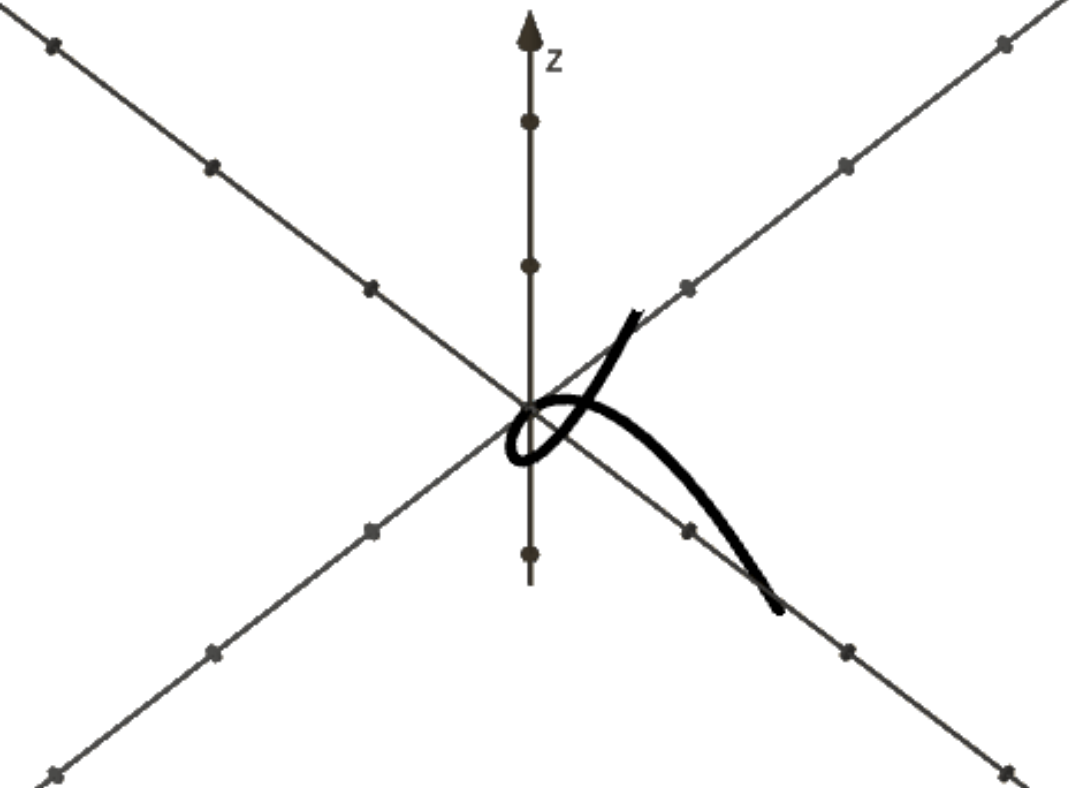
\includegraphics[width=0.3\linewidth]{Imagenes/curva normal}
			\caption{Curva racional en la carta afín $U_0$ dada por $t\mapsto (t,t^2,t^3)$.}
			\label{fig:curva-normal}
		\end{figure}
	
		Por el teorema \ref{encajesubvariedades}, la aplicación $\nu_d=\varphi_{\oo(d)}$ es un encaje holomorfo llamado \textbf{encaje de Veronese}. Por lo tanto, el haz lineal $\oo(d)$ es un haz lineal muy amplio. En particular, el haz lineal $\oo(1)$ es un haz amplio de $\pp^n$. 
		
		Si consideremos las funciones de transición de $\oo(1)$ sobre $\pp^N$
		\begin{equation*}
			g_{ij}=\frac{z_i}{z_j}.
		\end{equation*}
		Entonces las funciones de transición del pullback $v_d^*\oo(1)$ están dadas por
		\begin{equation*}
			(v_d^*g)_{ij}=g_{ij}\circ v_d=\frac{z_i^d}{z_j^d}.
		\end{equation*}
		Esto implica que 
		\begin{equation*}
			v_d^*\oo(1)\cong\oo(d)
		\end{equation*}
		como haces lineales sobre $\pp^n$.
	\end{example}
	
	\chapter{Algebrización de Variedades Complejas}

	Hasta este punto hemos introducido diversas herramientas cuya motivación está dada por la pregunta: ¿cuándo puede una variedad compleja describirse mediante ecuaciones algebraicas?
	
	\begin{definition}
		Una variedad compleja se dice \textbf{algebrizable}, o se dice que \textbf{admite una estructura algebraica}, si es biholomorfa a una variedad algebraica $V\subset \pp^N$.
	\end{definition}
	
	Si $M$ es una variedad compleja algebrizable, a la variedad algebraica $V\subset \pp^N$ se le denomina \textbf{realización} de $M$\footnote{También se suele decir que $M$ se \textbf{realiza} como la variedad algebraica $V$.}. Por el Teorema \ref{varalg}, toda variedad algebraica es conexa y compacta; y en consecuencia, en todo este trabajo nos hemos enfocado principalmente en variedades complejas con estas propiedades topológicas, pues toda variedad compleja algebrizable necesariamente debe ser conexa y compacta.
	
	En este último capítulo retomaremos todas las herramientas introducidas anteriormente para darle sentido a la pregunta de algebrización y exponer los criterios que nos permiten determinar cuándo una variedad compleja admite una estructura algebraica.

    \section{Subvariedades Analíticas}
    
    Antes de estudiar la algebrización de variedades, debemos introducir los últimos objetos fundamentales del trabajo.
    
    \begin{definition}[Subconjunto analítico]
    	Sea $M$ una variedad compleja. Un \textbf{subconjunto analítico} de $M$ es un subconjunto cerrado $V\subset M$ con la siguiente propiedad: para cada punto $x\in V$ existe una vecindad $U\subset M$ de $x$ tal que
    	\begin{equation*}
    		U\cap V=\{z\in U:f_1(z)=\cdots=f_k(z)=0\}
    	\end{equation*}  
    	para algunas funciones holomorfas $f_1,\dots,f_k\in\oo_M(U)$.
    \end{definition}
    
    Todo conjuntos algebraico de $\cc$ o $\pp^n$ son subconjuntos analíticos. Así, los subconjuntos analíticos son una generalización de los conjuntos algebraicos para otras variedades complejas.
    
    \begin{definition}[No singular]
    	Sea $M$ una variedad compleja y $V$ un subconjunto analítico de $M$. Decimos que $x\in V$ es \textbf{regular} o \textbf{no singular} si existe una carta $(U,\varphi)$ de $M$ alrededor de $x$ tal que $U\cap V=Z(f_1,\dots,f_k)$ y $\varphi(x)\in \varphi(U)$ es un punto regular de la aplicación
    	\begin{equation*}
    		f:=(f_1\circ\varphi^{-1},\dots,f_k\circ\varphi^{-1}):\varphi(U)\longrightarrow \cc^k.
    	\end{equation*}
    	Es decir, la jacobiana de $f$ en $\varphi(x)$ tiene rango $k$. Denotamos por $V^*$ al conjunto de todos los puntos regulares de $V$.
    	
    	Los puntos del conjunto $V_s:=V\setminus V^*$ son llamados \textbf{puntos singulares}. Por último, decimos que $V$ es \textbf{no singular} si $V_s=\emptyset$, es decir, si $V$ es una subvariedad compleja de $M$ (véase observación \ref{subvariedadesporecuaciones}).
    \end{definition}
    
    Los subconjuntos analíticos pueden interpretarse como variedades complejas que permiten singularidades. Aunque estas singularidades serán solo un subconjunto cerrado y al igual que las variedades algebraicas, los puntos regulares formarán un subconjunto denso. Esto implica que las subvariedades analíticas se comportan como subvariedades complejas con una muy pequeña cantidad\footnote{Puede ser infinita numerable si la variedad es no compacta.} de singularidades.
    
    \begin{propo}\parencite[Chap 0, Sec. 2.2]{griffiths}\label{puntossingulares}
    	Sea $M$ una variedad compleja y $V\subset M$ un subconjunto analítico. Entonces el conjunto de puntos singulares $V_s$ está contenido en un subconjunto analítico de $M$ no igual a $V$.
    \end{propo} 
%    \begin{proof}
%    	Tomemos $p\in V$ y una vecindad $U$ de $p$ tal que
%    	\begin{equation*}
%    		V\cap U=Z(f_1,\dots, f_r),\qquad f_i\in\oo_M(U).
%    	\end{equation*}
%    	Sea $J(f)$ la matriz jacobiana de la aplicación $f=(f_1,\dots,f_r)$. Definamos
%    	\begin{equation*}
%    		k=\max_{q\in V\cap U}\operatorname{rk} J(f)(q).
%    	\end{equation*}
%    	Entonces el conjunto
%    	\begin{equation*}
%    		W=\{q\in V\cap U:\mathrm{rk}J(f)(q)<k\}
%    	\end{equation*}
%    	está definido por la anulación de todos los menores $k\times k$, por lo que es un subconjunto analítico de $V\cap U$. En particular, $W\neq V\cap U$ pues existe al menos una menor $k\times k$ que no se anula idénticamente en $V\cap U$. De esta manera,
%    	\begin{equation*}
%    		V_s\cap U\subset W.
%    	\end{equation*}
%    	Por lo tanto, $V_s$ está contenido en un subconjunto analítico no igual a $V$.
%    \end{proof}
    
%    \begin{remark}
%    	Sea $V$ un subconjunto analítico de $M$ y $p\in V$ un punto no singular. Por definición, existe una vecindad $U$ de $p$ tal que
%    	\begin{equation*}
%    		V\cap U=Z(f_1,\cdots,f_k)
%    	\end{equation*}
%    	donde la función inducida en una carta tiene rango $k$. En particular, $p$ es un punto regular de $f$ y $f^{-1}(p)=V\cap U$ es una variedad compleja de dimensión $k$ (falta cita). Así, definimos 
%    	\begin{eqnarray*}
%    		\dim_p V:= k.
%    	\end{eqnarray*}
%    \end{remark}
   
    \begin{example}
    	Consideremos $D\subset \cc^n$ un conjunto discreto y cerrado no vacío. Esto significa que para todo punto $p=(p_1,\dots,p_n)\in D$ existe una vecindad del punto $U\subset\cc^n$ tal que
    	\begin{equation*}
    		U\cap D =\{p\}.
    	\end{equation*} 
    	Notemos que $Z(z_1-p_1,\cdots,z_n-p_n)=\{p\}$. Por lo tanto, $D$ es un subconjunto analítico de $\cc^n$.
    \end{example}
    
    \begin{remark}
    	Sabemos que los conjuntos algebraicos de $\mathbb{A}^1_\cc$ solo son conjuntos finitos. Por el ejemplo anterior, cualquier conjunto discreto $D$ en $\cc$ es analítico. Por lo tanto, los conjuntos algebraicos de  $\mathbb{A}^1_\cc$ también son analíticos, pero además, existen subconjuntos analíticos que no son algebraicos (véase ejemplo \ref{graficadelseno}).
    \end{remark}
    
    \begin{lemma}\label{preimagen analitico}
    	Sea $f:N\to M$ una aplicación holomorfa y $V\subset M$ un subconjunto analítico. Entonces $f^{-1}(V)\subset N$ es un subconjunto analítico.
    \end{lemma}
    \begin{proof}
    	Sea $V\subset M$ un subconjunto analítico y definamos $W=f^{-1}(V)$. Consideremos $p\in W$, entonces $f(p)\in V$. Como $V$ es analítico, existe una vecindad $U$ de $f(p)$ tal que
    	\begin{equation*}
    		U\cap V=Z(f_1,\dots,f_k)
    	\end{equation*} 
    	donde $f_1,\dots,f_k\in\oo_M(U)$. Luego, como $f$ es continua, $U'=f^{-1}(U)$ es una vecindad abierta de $p$. Definamos las funciones
    	\begin{equation*}
    		g_i=f_i\circ f:U'\to\cc,\quad i=1,2,\dots,k.
    	\end{equation*}
    	Notemos que las funciones $g_i$ son holomorfas, por ser composición de aplicaciones holomorfas. Así, 
    	\begin{align*}
    		U'\cap W&=f^{-1}(U\cap V)\\
    		&=f^{-1}(Z(f_1,\dots,f_k))\\
    		&=f^{-1}\left(\bigcap_{i=1}^k Z(f_i) \right)\\
    		&= \bigcap_{i=1}^k f^{-1}(Z(f_i))\\
    		&=\bigcap_{i=1}^k Z(f_i\circ f)\\
    		&=\bigcap_{i=1}^k Z(g_i)\\
    		&=Z(g_1,\dots,g_k).
    	\end{align*}
    	Por lo tanto, $W=f^{-1}(V)$ es un subconjunto analítico.
    \end{proof}
    
    \begin{definition}
    	Sea $M$ una variedad compleja y $V$ un subconjunto analítico de $M$. Decimos que $V$ es \textbf{irreducible} si no es posible escribirla como una unión $V=V_1\cup V_2$ de dos subconjuntos analíticos propios $V_i\subset V$ de $M$.\\
    	Un subconjunto analítico irreducible es llamado \textbf{subvariedad analítica}.
    \end{definition}
    
    \begin{corollary}
    	Sea $M$ una variedad compleja y $V$ un subconjunto analítico de $M$. Entonces el conjunto $V^*$ es denso en $V$ y una subvariedad compleja no vacía de $M$.
    \end{corollary}
    \begin{proof}
    	Supongamos que $V$ es irreducible. Sea $p\in V$ un punto regular, entonces existe una vecindad $U$ de $p$ tal que $V\cap U\subset V^*$ es una subvariedad compleja de $U$. De esta manera, $p$ es un punto interior de $V^*$. Con lo cual, $V^*$ es un abierto. 
    	
    	Por la proposición \ref{puntossingulares}, sabemos que existe un subconjunto analítico $W$ tal que
    	\begin{equation*}
    		V_s\subset W\subsetneq V.
    	\end{equation*}
    	Como $W\neq V$, entonces $V^*=V\setminus V_s$ es no vacío. En particular, $V^*$ es una subvariedad compleja no vacía.
    	
    	Supongamos que $V_s$ contiene un abierto no vacío $A\subset V$. Entonces $A\subset W$. Dado que $V$ es irreducible y $W$ es un subconjunto analítico propio, por el teorema de la identidad, las funciones que definen a $W$ cerca de $A$ se deben anular siempre. Esto implica que $W=V$, lo cual es una contradicción. Con lo cual, $A$ es vacío.
    	
    	Si $V_s$ contuviera un abierto no vacío de $V$, entonces también lo contiene el subconjunto analítico $W$. Sin embargo, un subconjunto analítico propio de un subconjunto analítico irreducible no puede contener un abierto relativo. Por lo que, $V_s$ no contiene abiertos de $V$
    	
    	Como $V_s$ es cerrado en $V$ y no contiene abiertos de $V$, entonces
    	\begin{equation*}
    		\mathrm{Int}(V_s)=\emptyset.
    	\end{equation*}
    	Con lo cual, $V^*=V\setminus V_s$ es denso en $V$.
    	
    	Si $V$ no es irreducible, se aplica el argumento a cada componente irreducible $V_i$. Obteniendo que $V_i^*$ es denso en $V_i$, y por tanto la unión de todos los puntos regulares es densa en $V$.
    \end{proof}
    
    \begin{definition}
    	Sea $V\subset M$ una subvariedad analítica. Definimos la \textbf{dimensión} de $V\subset M$ como
    	\begin{equation*}
    		\dim V:=\dim V^*.
    	\end{equation*}
    	Es decir, la dimensión como subvariedad compleja de sus puntos no singulares.
    	
    	De igual manera, definimos la \textbf{codimensión} de $V$ como la codimensión de $V^*$.
    	Una \textbf{hipersuperficie analítica} es una subvariedad analítica de codimensión uno.
    \end{definition}
    
    \begin{remark}
    	Una consecuencia directa de la geometría local (véase proposición \ref{hipersuperficiesenCn}), es que toda hipersuperficie analítica en una variedad compleja $M$ está definida localmente como el conjunto de ceros de una sola función. Es decir, si $H\subset M$ es una hipersuperficie analítica, entonces para todo punto $p\in H$ existe una vecindad $U$ de $p$ y una función holomorfa $f\in \oo_M(U)$ irreducible tal que
    	\begin{equation*}
    		H\cap U=Z(f).
    	\end{equation*}
    \end{remark}
    
    \begin{example}
    	Consideremos la función holomorfa $y^2-x^2-x^3$ en $\cc^2$. Su conjunto de ceros es un subconjunto analítico en $\cc^2$, y de hecho es irreducible, por lo que
    	\begin{equation*}
    		Z(y^2-x^2-x^3)\subset\cc^2
    	\end{equation*}
    	es una subvariedad analítica irreducible (de hecho también algebraica) de $\cc^2$. En una vecindad suficientemente pequeña del origen, la función $\sqrt{1+x}$ es holomorfa. De esta manera, como
    	\begin{equation*}
    		y^2-x^2-x^3=(y-x\sqrt{1+x})(y+x\sqrt{1+x}),
    	\end{equation*}
    	el germen de la subvariedad es reducible. Por lo tanto, existen dos componentes irreducibles localmente definidas por los factores $y\pm x\sqrt{1+x}$.
    	\begin{figure}[H]
    		\centering
    		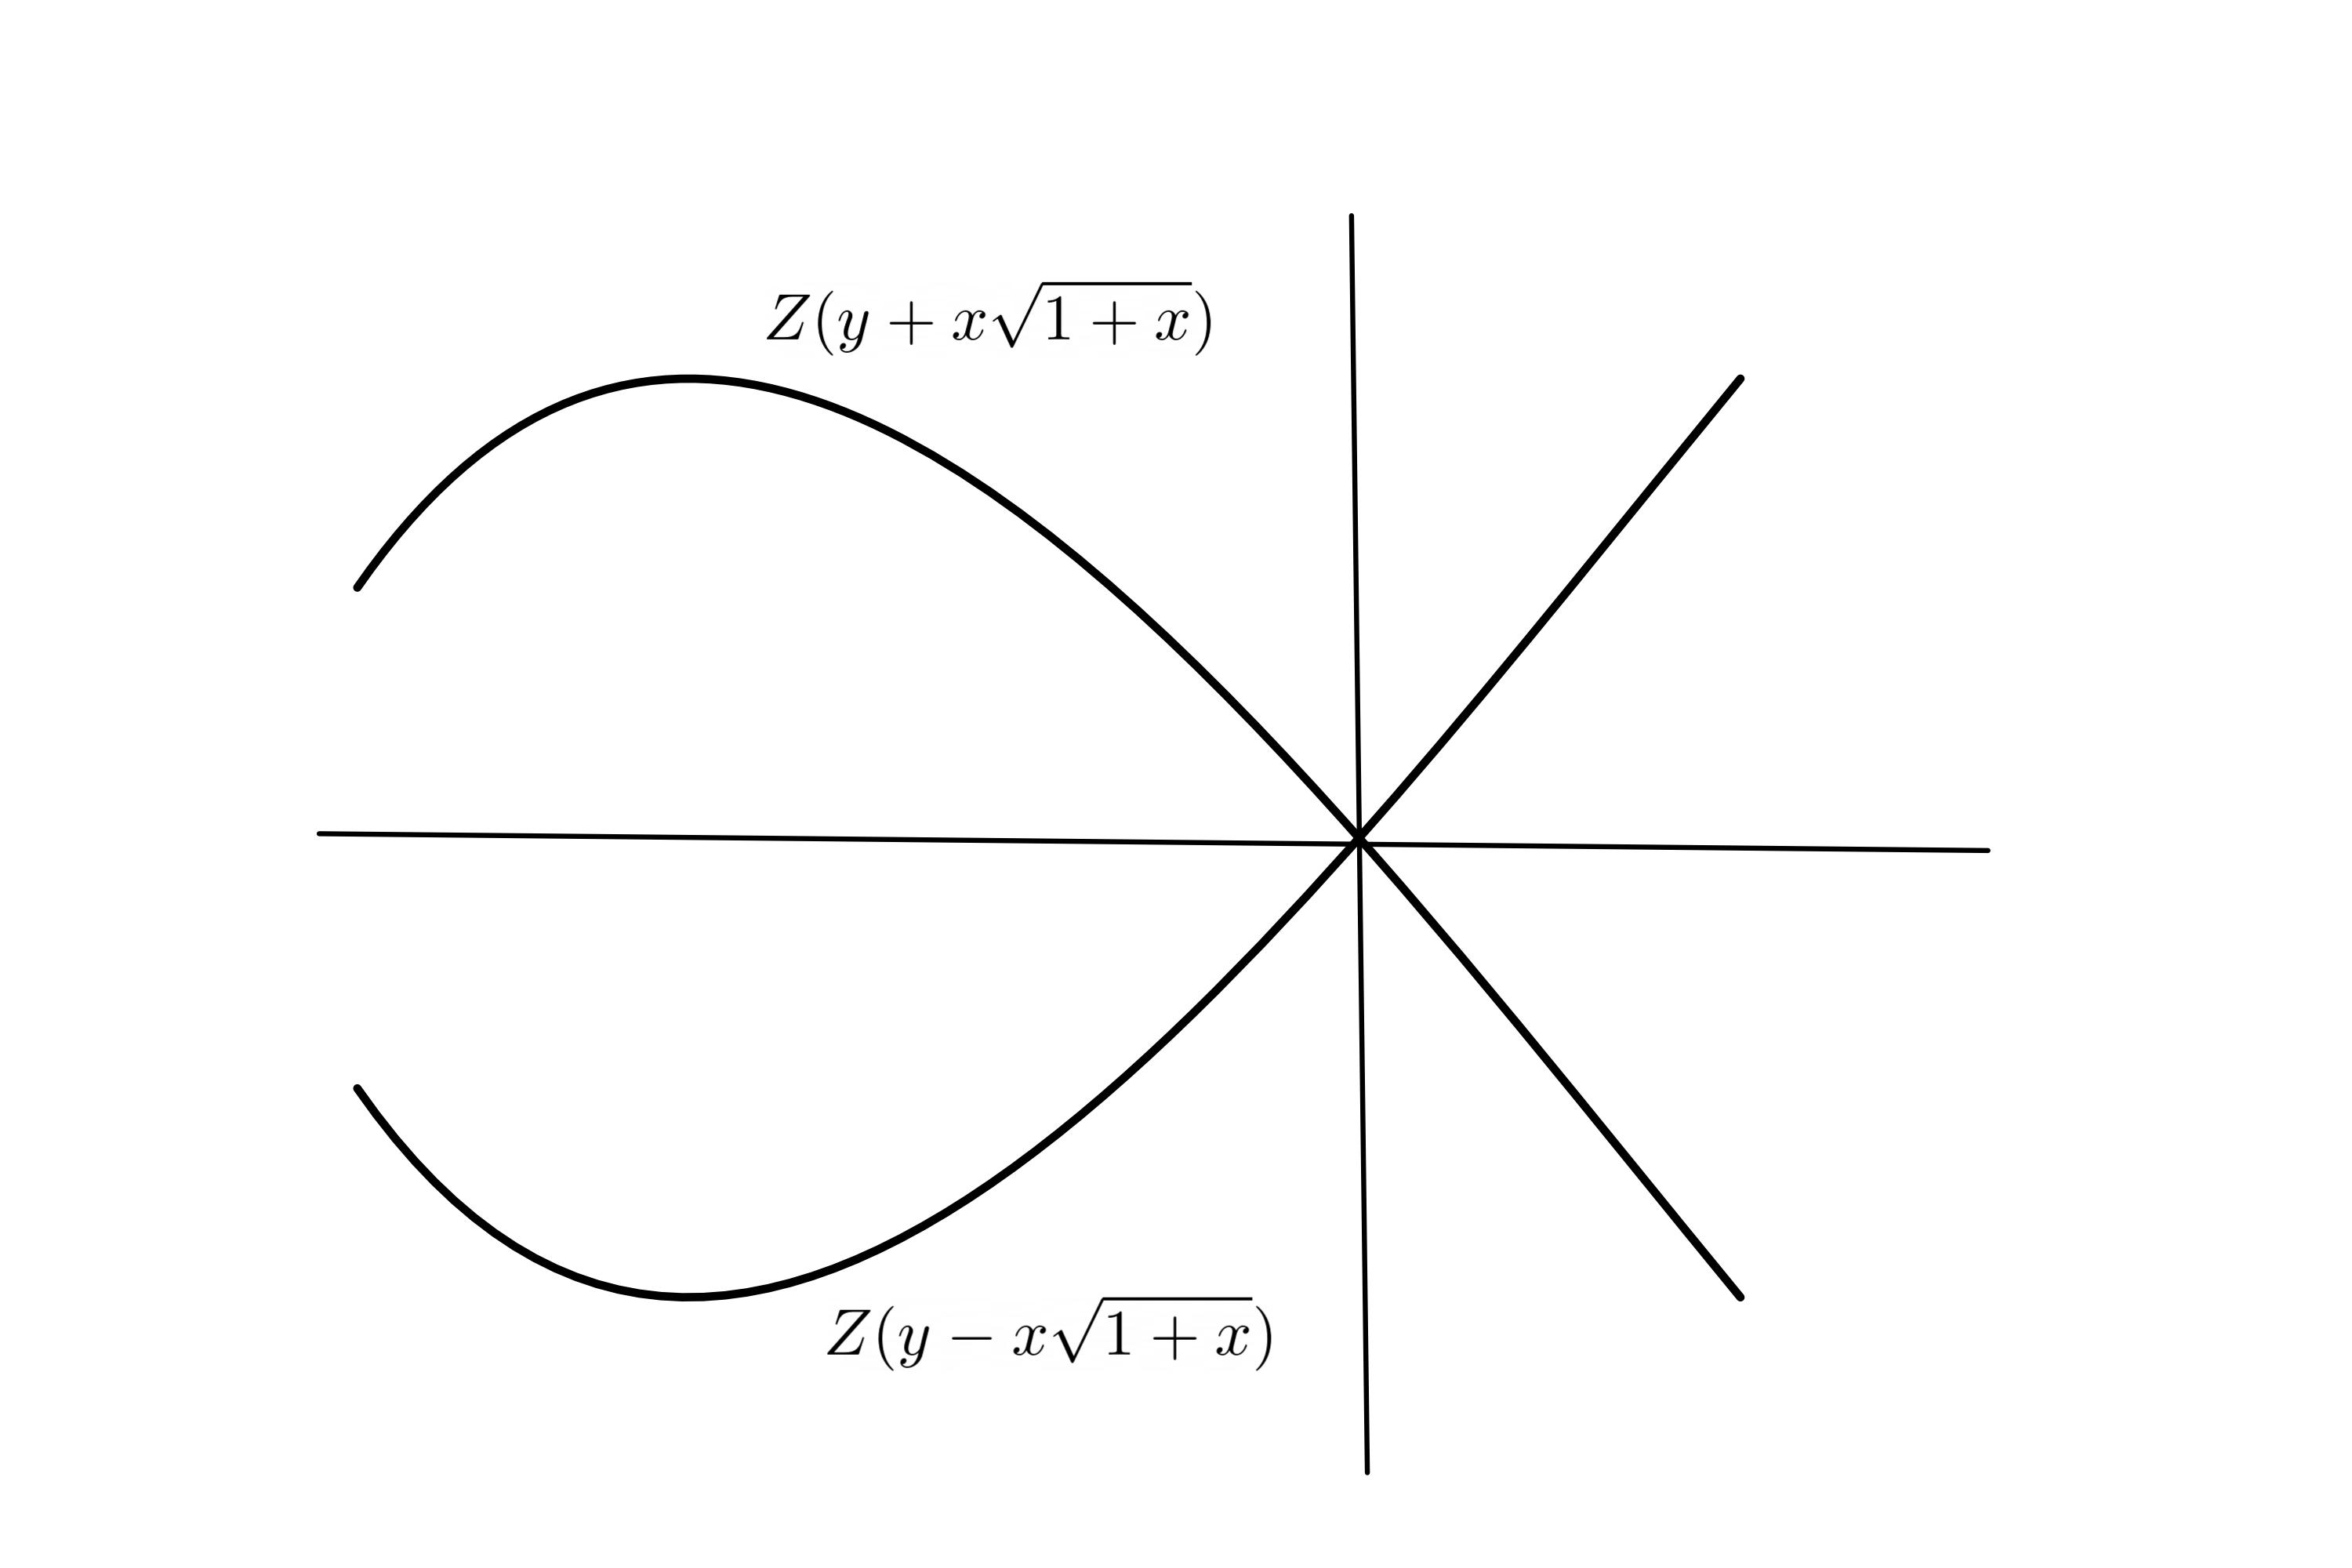
\includegraphics[width=0.5\linewidth]{Imagenes/componenteslocales}
    		\caption{Componentes irreducibles locales de $Z(y^2-x^2-x^3)$.}
    		\label{fig:componenteslocales}
    	\end{figure}
    	
    \end{example}
    
    Por último, presentaremos uno de los resultados más importantes de las subvariedades analíticas:
    
    \begin{theorem}\parencite[Chap 0, Sec. 2.2]{griffiths}\label{irreducibleconexo}
    	Sea $M$ una variedad compleja y $V\subset M$ un subconjunto analítico. Entonces $V$ es irreducible si, y solo si, $V^*$ es conexa.
    \end{theorem}
	
    \subsection{Teoremas de Remmert}
		
		Los subconjuntos analíticos son objetos muy importantes en la geometría algebraica y el análisis complejo. Sin embargo, describir su comportamiento es una tarea lejos de ser trivial y llevó a muchos matemáticos a estudiar en profundidad estos objetos.
		
		Los teoremas de \textit{Remmert} describen el comportamiento de los subconjuntos analíticos bajo imágenes y cerradura. El \textit{teorema de la aplicación propia} nos garantiza que la imagen de un subconjunto analítico por una aplicación holomorfa propia es nuevamente un subconjunto analítico, mientras que el \textit{teorema de Remmert-Stein} describe las condiciones para que la cerradura de un subconjunto analítico siga siendo analítico.
		
		Estos resultados son importantes para la teoría de subconjuntos analíticos y funcionan como herramientas esenciales en nuestro entendimiento de los encajes de variedades complejas. Solo nos limitaremos a enunciar ambos teoremas, remitiendo al lector a las referencias clásicas para entender sus demostraciones (véase \parencite{griffiths}, \parencite{lojasiewicz} y \parencite{chirka}). 
		
    	\begin{theorem}[de la aplicación propia de Remmert]\label{aplicacionpropia}
    		Sea $f:M\to N$ una aplicación holomorfa propia\footnote{Recordemos que una aplicación propia es una función continua entre espacios topológicos cuya preimagen de conjuntos compactos es compacta.} entre variedades complejas. Si $V$ es un subconjunto analítico de $M$, entonces $f(V)$ es un subconjunto analítico de $N$.
    	\end{theorem}
    	Una demostración puede consultarse en el libro \parencite[Chap.3~,Sec.2]{griffiths}, donde se basa fuertemente en una versión particular del teorema de Remmert-Stein llamado \textbf{teorema de Extensión de Levi (II)} y muchas técnicas del análisis complejo. Otra demostración, de carácter más geométrico, fue dada por Chirka \parencite[Chap. 4~, Sec.4.4]{chirka}.
    	
		
		\begin{theorem}[de Remmert-Stein para variedades complejas]\label{remmertstein}
			Sea $M$ una variedad compleja conexa de dimensión $n$ y $Z\subset M$ un subconjunto analítico de codimensión menor a $k+1$. Si $V\subset M\setminus Z$ es un subconjunto analítico de codimensión $k$, entonces la cerradura $\overline{V}$ en $M$ es un subconjunto analítico. 
		\end{theorem}
		
		Para probar este teorema se hace una reducción local del mismo. En primer lugar, por la proposición \ref{puntossingulares}, el conjunto de puntos singulares de $Z$ está contenido en un subconjunto analítico propio $Z_1$. Asimismo, los puntos singulares de $Z_1$ están contenidos en un subconjunto analítico propio $Z_2\subset Z_1$. De esta manera, tenemos la siguiente cadena de subconjuntos analíticos
		\begin{equation*}
			Z=Z_0\supset Z_1 \supset Z_2 \supset \cdots 
		\end{equation*}
		con cada $Z_j\setminus Z_{j+1}$ una subvariedad compleja de codimensión $\geq k$ en $M$. Como cada $Z_{j+1}$ es un subconjunto analítico propio de $Z_j$, su dimensión es estrictamente menor, por lo tanto, el proceso termina después de un número finito de pasos. Entonces existe un $r\in\nn$ tal que $Z_{r+1}=\emptyset$. De esta manera, podemos extender $V$ sucesivamente en cada subvariedad $Z_{j}\setminus Z_{j+1}$, primero tomando la cerradura en $M\setminus Z_{1}$, luego en $M\setminus Z_2$ y continuando una cantidad finita de veces. Con lo cual, es suficiente probarlo suponiendo que $Z\subset M$ es una subvariedad compleja de codimensión $\geq k$.
		
		En segundo lugar, para probar que $\overline{V}$ es analítico, es suficiente mostrar que lo es en una vecindad para cualquiera de sus puntos. Por lo tanto, podemos suponer que $M$ es un polidisco de $\cc^n$ que contiene al origen y $0\in Z$. Después de un cambio de coordenadas,  podemos ver que la subvariedad $Z$ es de la forma $Z=Z(z_1,z_2,\dots,z_{k+1})$. De esta manera, tenemos la reducción local del teorema:
		
		\begin{propo}
			Sean $D\subset\cc^n$ un polidisco que contiene al origen y $Z=Z(z_1,z_2,\dots,z_{k+1})$. Si $V$ es un subconjunto analítico de $D\setminus Z$ de codimensión $k$, entonces $\overline{V}$ es un subconjunto analítico de $D$.
		\end{propo}
		
		\begin{remark}
			El teorema de Remmert-Stein puede ser visto como una generalización geométrica del teorema de Hartogs. Una versión del teorema de Hartogs nos dice que si $f$ es una función holomorfa en $M\setminus\{p\}$, y $\dim M\geq 2$, entonces $f$ se extiende holomorficamente a toda $M$ (véase \parencite[Chap. 2, Sec. 1, Cor. 2.1.6]{huybrechts2005complex}).
			
			En esta misma situación, la gráfica
			\begin{equation*}
				\Gamma_f=\{(x,f(x)):x\in M\setminus \{p\}\}\subset (M\setminus \{p\})\times \cc,
			\end{equation*}
			es un subconjunto analítico. Así, el teorema de Remmert-Stein nos dice que la cerradura $\overline{\Gamma_f}$ es un subconjunto analítico de $M\times \cc$. En particular, $\overline{\Gamma_f}$ resulta ser la gráfica de una función holomorfa
			\begin{equation*}
				\tilde{f}\in\oo_M(M)
			\end{equation*}
			tal que $\tilde{f}|_{M\setminus\{p\}}=f$. Este es exactamente el mismo resultado que nos da Hartogs. 
		\end{remark}
		
    \section{Teorema de Chow}
    
	Hemos estudiado las subvariedades analíticas y visto muchas propiedades interesantes de ellas. Para el objetivo de buscar la algebrización de variedades complejas, vimos que las imágenes de subvariedades analíticas son analíticas (\ref{aplicacionpropia}). Así, un encaje de una variedad compleja al espacio proyectivo significa tener un biholomorfismo entre la variedad y una subvariedad analítica del espacio proyectivo. Por lo tanto, la última pregunta que nos interesa abordar resulta tanto natural como profunda. ¿Cómo son las subvariedades analíticas del espacio proyectivo?
	
	En 1949, \textit{Wei-Liang Chow} publicó su artículo \enquote{On Compact Complex Analytic Varieties}, en el cual demuestra un profundo resultado conocido actualmente como \textit{teorema de Chow} y responde a las cuestiones más importantes de todo este trabajo. La demostración de este resultado ha tenido una historia y desarrollo muy interesante durante el siglo pasado. El enfoque de Chow fue usar varias técnicas analíticas y topológicas, luego en 1953 Reinhold Remmert y Karl Stein presentaron una demostración más simple desarrollando un resultado relacionado con la cerradura de conjuntos analíticos. Tres años después, en 1956, \textit{Jean Pierre Serre} publicó su famoso artículo \textit{"Géométrie algébrique et géométrie analytique"}, bautizado como \textbf{GAGA}, y presentó una demostración muy elegante usando toda la nueva herramienta de gavillas coherentes que desarrolló en su artículo. En nuestro caso, presentaremos una demostración basada en la construcción de Remmert y Stein.

\begin{theorem}[Teorema de Chow]
	Todo subconjunto analítico del $n$-espacio proyectivo es algebraico.
\end{theorem}
	\begin{proof}\parencite{chirka}
		Sea $X\subset \pp^n$ un subconjunto analítico. Consideremos la proyección usual
		\begin{align*}
			\pi:\cc^{n+1}\setminus\{0\}\longrightarrow \pp^n
		\end{align*}
		Tomando $V_0=\pi^{-1}(X)\subset \cc^{n+1}\setminus\{0\}$, entonces $V_0$ es un subconjunto analítico (\ref{preimagen analitico}) de $\cc^{n+1}\setminus\{0\}$. Por el teorema de Remmert-Stein \ref{remmertstein}, la cerradura 
		\begin{equation*}
			V=\overline{V_0}=V_0\cup\{0\}
		\end{equation*}
		es un subconjunto analítico de $\cc^{n+1}$.\\
		Ahora, observemos que  si $z\in V$, entonces para todo $t\in\cc$ tenemos que $tz\in V$. Esto significa que $V$ es un cono complejo.
		
		Como $0\in V$, entonces existe una vecindad $U\subset\cc^{n+1}$ de $0$ y $f_1,\dots,f_k\in\mathscr{O}_{\cc^{n+1}}(U)$ tales que 
		\begin{equation*}
			V\cap U=Z(f_1,\dots,f_k).
		\end{equation*}
		Sea $I=\langle \overline{f_1},\dots,\overline{f_k} \rangle\subset \mathscr{O}_{n+1}$ el ideal de gérmenes. Si $\overline{f}\in I$, entonces $f$ se puede escribir como 
		\begin{equation*}
			f(z)=\sum_{i=0}^{\infty}h_i(z)
		\end{equation*}
		donde $h_i\in\cc[z_0,\dots,z_n]_{(i)}$ son polinomios homogéneos de grado $i$.\\
		Sea $z\in V$ y $|\lambda|<1$, entonces 
		\begin{equation*}
			0=f(\lambda z)=\sum_{i=0}^{\infty}h_i(\lambda z)=\sum_{i=0}^{\infty}\lambda^ih_i( z)
		\end{equation*}
		Como $f(\lambda z)$ es holomorfa en $\lambda$, entonces por el teorema de la identidad $h_i(z)=0$ para todo $i\in\nn$. Con esto, $\overline{h_i}\in I$.\\
		Así, $I$ está generado por polinomios homogéneos. Como $\mathscr{O}_{n+1}$ es noetheriano (véase teorema \ref{anillonoetheriano}), $I$ es finitamente generado. Esto significa que existen $F_1,\dots, F_m\in\cc[z_0,\dots,z_n]$ polinomios homogéneos tal que $I=\langle F_1,\dots, F_m \rangle$.
		Por lo tanto, $X=Z(F_1,\dots,F_m)$.
	\end{proof}
	
	Supongamos que $M$ admite un haz lineal amplio $L\longrightarrow M$, entonces existe un encaje holomorfo a algún espacio proyectivo $\varphi:M\hookrightarrow\pp^N$
	\[\begin{tikzcd}
		L \\
		\\
		M && {\mathbb{P}^N}
		\arrow[no head, from=1-1, to=3-1]
		\arrow[hook, from=3-1, to=3-3]
	\end{tikzcd}\]
	Como $\varphi$ es un encaje, $\varphi(M)$ es biholomorfo a $M$. Por el teorema de la aplicación propia (\ref{aplicacionpropia}), $\varphi(M)\subset\pp^N$ es una subvariedad analítica. Por el teorema de Chow, $\varphi(M)$ es una variedad algebraica. Por lo tanto, podemos concluir que:

\begin{corollary}
	Toda variedad compleja que admite un haz amplio es algebraica.
\end{corollary}

	Como observamos en el capítulo \ref{cap2}, en geometría compleja no existe un resultado general análogo al teorema de Whitney. Por ello, resulta natural buscar encajes en un espacio tan familiar y estructurado como lo es el espacio proyectivo complejo \(\mathbb{P}^N\). Sin embargo, el teorema de Chow nos muestra que la posibilidad de realizar una variedad compleja como subvariedad proyectiva es una propiedad exclusiva de las variedades algebrizables.
	
	En geometría algebraica, una variedad proyectiva se entiende como una subvariedad algebraica del espacio proyectivo. En nuestra definición, toda variedad proyectiva admite un encaje en un espacio proyectivo complejo; por el Teorema \ref{proyectivossiamplio}, dicha variedad es algebraica. Por lo tanto, nuestra definición de variedad proyectiva coincide con la noción clásica de la geometría algebraica.

	\begin{corollary}\label{teoriemann}
		Toda superficie de Riemann compacta es algebraica.
	\end{corollary}
	
	Con ello observamos que toda superficie de Riemann compacta puede realizarse como una variedad algebraica de dimensión $1$, es decir, como una curva algebraica. Sin embargo, estos resultados son solo teórico y no constituyen, por sí mismos, un método directo para determinar ecuaciones explícitas de una variedad compleja. De hecho, existe una rama activa de las matemáticas dedicada precisamente a construir y estudiar ecuaciones asociadas a superficies de Riemann; un ejemplo clásico de esta perspectiva es la teoría de las curvas modulares.
	
	\begin{example}\parencite{curvaselipticas}
		Consideremos la superficie de Riemann
		\[
		T=\cc/\Lambda,
		\]
		donde $\Lambda=\omega_1\zz+\omega_2\zz$ es una retícula de $\cc$. A este retículo le asociamos la \textbf{función de Weierstrass} $\wp$, que desciende a una función meromorfa en $T$ y está dada por
		\[
		\wp(z)=\frac{1}{z^2}+\sum_{\omega\in\Lambda\setminus\{0\}}
		\left(\frac{1}{(z-\omega)^2}-\frac{1}{\omega^2}\right).
		\]
		Su derivada satisface la relación
		\[
		(\wp'(z))^2=4\wp(z)^3-g_2\wp(z)-g_3,
		\]
		donde $g_2$ y $g_3$ son constantes que dependen de $\Lambda$ y vienen dadas por las \textbf{series de Eisenstein}
		\[
		g_2=60\sum_{\omega\in\Lambda\setminus\{0\}}\frac{1}{\omega^4},
		\qquad
		g_3=140\sum_{\omega\in\Lambda\setminus\{0\}}\frac{1}{\omega^6}.
		\]
		Con esto, obtenemos una aplicación holomorfa bien definida
		\[
		\phi:T\longrightarrow \pp^2,\qquad
		z\longmapsto [\wp(z):\wp(z)^2:1],
		\]
		la cual define un encaje holomorfo. Así, se obtiene un biholomorfismo entre el toro $T$ y la curva elíptica dada por la ecuación
		\[
		4y^2=4x^3-g_2x-g_3.
		\]
		En general, se puede probar que toda superficie de Riemann de género $1$ está dada por la ecuación afín
		\begin{equation*}
			y^2=x(x-1)(x-\lambda),\qquad \text{para todo }\ \lambda\in\cc\setminus\{0,1\}. 
		\end{equation*}
	\end{example}

	\begin{example}[Encaje de Segre]
		Consideremos la superficie compleja $M=\pp^1\times\pp^1$ y denotemos por $p_1:M\to \pp^1$ y $p_2:M\to \pp^1$ las proyecciones de $M$. Por el teorema \ref{seccionesproyectivo}, sabemos que
		\begin{equation*}
			H^0(\pp^1,\oo(1))\cong\langle x_0,x_1\rangle, \qquad H^0(\pp^1,\oo(1))\cong\langle y_0,y_1\rangle.
		\end{equation*}
		Además, el pullback de las secciones bajo las proyecciones vuelven a ser los monomios $x_0,x_1,y_0,y_1$. De esta manera, las secciones $x_0$ y $x_1$ son linealmente independientes en $H^0(M,p_1^*\oo(1))$, y análogo con $y_0$ y $y_1$. Por lo que, estas secciones definen un subespacio lineal
		\begin{equation*}
			\cc[x_0,x_1]_{(1)}\otimes \cc[y_0,y_1]_{(1)}=\langle x_0,x_1\rangle\otimes \langle y_0,y_1\rangle\subset H^0(M,p_1^*\oo(1))\otimes H^0(M,p_2^*\oo(1)).
		\end{equation*}
		Definamos el haz lineal $L=p_1^*\oo(1)\otimes p_2^*\oo(1)$. Entonces, las secciones
		\begin{equation*}
			x_0\otimes y_0,\enspace x_0\otimes y_1,\enspace x_1\otimes y_0,\enspace x_1\otimes y_1
		\end{equation*}
		definen secciones linealmente independientes de $H^0(M,L)$. Usando el isomorfismo
		\begin{align*}
			\cc[x_0,x_1]\otimes \cc[y_0,y_1]\cong \cc[x_0,x_1,y_0,y_1]
		\end{align*}
		obtenemos que los productos 
		\begin{equation*}
			x_0y_0,\enspace x_0y_1,\enspace x_1y_0,\enspace x_1y_1
		\end{equation*}
		definen secciones linealmente independientes de $H^0(M,L)$. Con lo cual, obtenemos el morfismo inducido por estas secciones
		\begin{align*}
				&\sigma:\pp^1\times\pp^1\longrightarrow \pp^3\\
			([x_0:x_1],[y_0:&y_1])\mapsto [x_0y_0:x_0y_1:x_1y_0:x_1y_1]
		\end{align*}

		Notemos que la aplicación $\sigma$ es holomorfa, pues sus coordenadas homogéneas son productos de coordenadas homogéneas en cada factor. Para probar que $\sigma$ es un encaje holomorfo, estudiaremos su expresión en cartas afines. Consideremos las cartas estándar de $\pp^1$
		\begin{align*}
			&U_0=\{[x_0:x_1]:x_0\neq 0\},\qquad U_1=\{[x_0:x_1]:x_1\neq 0\},\\
			&V_0=\{[y_0:y_1]:y_0\neq 0\},\qquad V_1=\{[y_0:y_1]:y_1\neq 0\}.
		\end{align*}
		En $U_0\times V_0$ tenemos las coordenadas afines $(s,t)$ donde
		\begin{equation*}
			s=\frac{x_1}{x_0},\qquad t=\frac{y_1}{y_0}.
		\end{equation*}
		Dado que 
		\begin{equation*}
			[x_0y_0:x_0y_1:x_1y_0:x_1y_1]=\left[ 1:\frac{y_1}{y_0}:\frac{x_1}{x_0}:\frac{x_1y_1}{x_0y_0}\right],
		\end{equation*}
		entonces en las coordenadas $(s,t)$ la aplicación $\sigma$ queda dada como
		\begin{equation*}
			(s,t)\longmapsto [1:t:s:st].
		\end{equation*}
		Por tanto, sobre la carta afín $Z(X_0)^c\subset\pp^3$, la inversa de $\sigma$ sobre su imagen viene dada por
		\begin{equation*}
			[X_0:X_1:X_2:X_3]\longmapsto \left([1:X_2/X_0],[1:X_1/X_0]\right),
		\end{equation*}
		la cual es holomorfa. Análogamente, en las otras tres cartas de $M$ se obtienen expresiones locales de $\sigma$ y de su inversa dadas por
		\begin{align*}
			&U_0\times V_1:\quad (s,t)\mapsto [t:1:st:s],\qquad
			[X]\mapsto \left([1:X_3/X_1],[X_0/X_1:1]\right),\\
			&U_1\times V_0:\quad (s,t)\mapsto [s:st:1:t],\qquad
			[X]\mapsto \left([X_0/X_2:1],[1:X_3/X_2]\right),\\
			&U_1\times V_1:\quad (s,t)\mapsto [st:s:t:1],\qquad
			[X]\mapsto \left([X_1/X_3:1],[X_2/X_3:1]\right).
		\end{align*}
		De aquí se sigue que $\sigma$ induce un biholomorfismo entre $M=\pp^1\times\pp^1$ y su imagen.
		
		Más aún, la imagen de $\sigma$ es la variedad algebraica proyectiva
		\begin{equation*}
			\sigma(M)=Z(X_0X_3-X_1X_2).
		\end{equation*}
		De esta manera, por la proposición \ref{encajesubvariedades}, la aplicación $\sigma$ es un encaje holomorfo.
		
		Por lo tanto, la superficie compleja $M=\pp^1\times\pp^1$ es algebrizable y la variedad algebraica asociada es
		\begin{equation*}
			V=Z(X_0X_3-X_1X_2)\subset\pp^3,
		\end{equation*}
			
%			Resta identificar la imagen. Si
%			\[
%			[X_0:X_1:X_2:X_3]=\sigma([u_0:u_1],[v_0:v_1]),
%			\]
%			entonces
%			\[
%			X_0X_3-X_1X_2
%			=
%			(u_0v_0)(u_1v_1)-(u_0v_1)(u_1v_0)=0,
%			\]
%			luego \(\sigma(\PP^1\times \PP^1)\subseteq V(X_0X_3-X_1X_2)\).
%			
%			Recíprocamente, si \([X_0:X_1:X_2:X_3]\in V(X_0X_3-X_1X_2)\), entonces la matriz
%			\[
%			\begin{pmatrix}
%				X_0 & X_1\\
%				X_2 & X_3
%			\end{pmatrix}
%			\]
%			tiene determinante cero, y por tanto rango a lo más uno. En consecuencia, dicha matriz se descompone como producto exterior de dos vectores no nulos de \(\CC^2\), es decir, existen \((u_0,u_1)\neq (0,0)\) y \((v_0,v_1)\neq (0,0)\) tales que
%			\[
%			\begin{pmatrix}
%				X_0 & X_1\\
%				X_2 & X_3
%			\end{pmatrix}
%			=
%			\begin{pmatrix}
%				u_0\\
%				u_1
%			\end{pmatrix}
%			\begin{pmatrix}
%				v_0 & v_1
%			\end{pmatrix}.
%			\]
%			Por lo tanto,
%			\[
%			[X_0:X_1:X_2:X_3]
%			=
%			[u_0v_0:u_0v_1:u_1v_0:u_1v_1]
%			\in \sigma(\PP^1\times\PP^1).
%			\]
%			Así,
%			\[
%			\sigma(\PP^1\times\PP^1)=V().
%			\]
%			

	\end{example}

\section{Otros criterios de algebrización}

En esta última sección presentaremos dos conceptos clave en la geometría compleja: las variedades de Moishezon y las variedades de Kähler. Ambos están profundamente relacionados con el problema de la algebrización. Sin embargo, para estudiarlos detalladamente necesitamos desarrollar herramientas más avanzadas que las desarrolladas hasta ahora.

La teoría de Moishezon se apoya en las funciones y aplicaciones meromorfas, las cuales surgen como un análogo a las funciones racionales y equivalencia birracional de la geometría algebraica. Por otro lado, la teoría de Kähler involucra técnicas de geometría diferencial, como métricas riemannianas, formas diferenciales, formas holomorfas y teorías de cohomología.

El objetivo no es desarrollar en profundidad estas teorías, sino presentar su importancia en la algebrización. Mientras que el trabajo de Moishezon estableció una relación muy profunda entre la geometría compleja con la algebraica, las variedades de Kähler lo hacen desde la geometría diferencial. De esta manera, esta sección funciona como una extensión conceptual del trabajo, orientada a mostrar conexiones con resultados más profundos de la geometría compleja.

\subsection{Variedades de Moishezon}

En geometría diferencial o algebraica, es común estudiar el comportamiento global de los objetos estudiando sus funciones. Sin embargo, notamos que las funciones holomorfas sobre variedades complejas conexas compactas (por ejemplo, las superficies de Riemann compactas) son constantes (\ref{holomorfasglobal}). Por lo que no podemos obtener información global de estas variedades a partir de sus funciones ¿Qué podemos hacer?

Las funciones meromorfas extienden el concepto de funciones holomorfas al permitir \enquote{polos controlados}, lo que enriquece aún más la estructura analítica de las variedades. Más aún, el conjunto de todas las funciones meromorfas forma un campo (véase proposición \ref{campodefunciones}), lo cual permite aplicar herramientas algebraicas más potentes. De esta manera, el estudio de las funciones meromorfas se vuelve esencial para comprender la estructura local y la geometría global de las variedades complejas.

\begin{definition}
	Sea $M$ una variedad compleja y $p\in M$. Definamos
	\begin{equation*}
		\mathcal{K}_{M,p}:=Q(\oo_{M,p})
	\end{equation*}
	donde $Q(\oo_{M,p})$ es el campo de fracciones asociado al dominio entero $\oo_{M,p}$ (véase corolario \ref{dominiolocal}). Esto es,
	\begin{equation*}
		\mathcal{K}_{M,p}=\left\{ \frac{f_p}{g_p}:f_p,g_p\in\oo_{M,p}\text{ y }g_p\neq 0\right\}.
	\end{equation*}
	Este campo es llamado \textbf{campo de funciones meromorfas} en $p$.
\end{definition}  

\begin{definition}
	Sea $M$ una variedad compleja. Una \textbf{función meromorfa} sobre $U\subset M$ es una aplicación
	\begin{equation*}
		f:U\longrightarrow \bigsqcup_{x\in U}\mathcal{K}_{M,x}
	\end{equation*}
	la cual asocia a $x\in U$ una función $f_x\in \mathcal{K}_{M,x}$ la cual cumple que para todo $p\in U$, existe una vecindad $V\subset U$ de $p$ y funciones holomorfas $g,h\in\oo_M(V)$, con $h\neq 0$, tal que $f|_V=\frac{g}{h}$\footnote{Esta igualdad significa que para todo $x\in V$ se tiene que $f(x)=\frac{g_x}{h_x}$.}.
\end{definition}

La \textbf{gavilla de funciones meromorfas} se denota por $\mathcal{K}_{M}$ y asigna a cada abierto $U$ el conjunto de funciones meromorfas sobre $U$.

\begin{propo}\label{campodefunciones}
	Sea $M$ una variedad compleja y $U\subset M$ un abierto conexo. Entonces $\mathcal{K}_{M}(U)$ es un campo.
\end{propo}
\begin{proof}
	Recordemos que la estructura de anillo de $\mathcal{K}_{M}(U)$ está dada punto a punto, es decir,
	\begin{align*}
		(f+g)(x):=f(x)+g(x)\in\mathcal{K}_{M,x}\\
		(fg)(x):=f(x)g(x)\in\mathcal{K}_{M,x}.
	\end{align*}
	y el elemento unidad es la función constante $1$ la cual es la fracción $1/1$ en cada campo $\mathcal{K}_{M,p}$.
	
	Sea $f\in \mathcal{K}_{M}(U)$ no cero. Buscamos un $f^{-1}\in\mathcal{K}_{M}(U)$ tal que $ff^{-1}=1$.
	Como $f\neq 0$, entonces existe un punto $p\in U$ tal que $f_p\in\mathcal{K}_{M,p}$ es no cero. Entonces existe una vecindad $V\subset U$ conexa de $p$ tal que
	\begin{equation*}
		f|_V=\frac gh,\qquad g,h\in\oo_M(V),\enspace h\neq 0,\enspace g_p\not\in\mathfrak{m}_p.
	\end{equation*}
	Es decir, $g_p\neq 0$ como germen en $p$. Notemos que el conjunto 
	\begin{equation*}
		Z=\{x\in V:g(x)=0\}
	\end{equation*}
	es un subconjunto analítico propio, esto es, $g$ no se puede anular en un abierto no vacío de $V$. Si $g$ se anulara en todo $V$, entonces $f|_V=0$ y contradice que $f_p\neq 0$.
	
	De esta manera, podemos definir la inversa localmente 
	\begin{equation*}
		f^{-1}|_V=\frac hg.
	\end{equation*} 
	Repetimos este proceso para cada punto donde el germen no sea nulo. Esto nos da una cubierta $\{W_i\}_{i\in I}$ de $U$ tal que
	\begin{equation*}
		f^{-1}|_{W_i}=\frac{h_i}{g_i}
	\end{equation*}
	está bien definida y satisfacen 
	\begin{equation*}
		f|_{W_i}f^{-1}|_{W_i}=1\in\mathcal{K}_M(W_i).
	\end{equation*}
	Notemos que además las funciones $f^{-1}|_{W_i}$ coinciden en las intersecciones $W_i\cap W_j$. Así, por la propiedad de sección global de la gavilla $\mathcal{K}_M$ tenemos que existe $f^{-1}\in \mathcal{K}_{M}(U)$ tal que
	\begin{equation*}
		ff^{-1}=1.
	\end{equation*}
\end{proof}

Si $M$ es una variedad compleja conexa, el espacio de secciones globales $\mathcal{K}_{M}(M)$ es llamado \textbf{campo de funciones meromorfas} sobre $M$ y lo denotamos por $\mathcal{K}(M)$. Este campo es de suma importancia para las variedades complejas y se relaciona con un teorema muy importante de la geometría compleja.

\begin{theorem}[Siegel]
	Sea $M$ una variedad compleja conexa compacta de dimensión $n$. Entonces
	\begin{equation*}
		\mathrm{trdeg}_\cc\mathcal{K}(M)\leq n.
	\end{equation*}
\end{theorem}
Una demostración detallada puede consultarse en \parencite[Teo. 4.23]{carlosga} y está basado en el lema de Schwarz de análisis complejo.

\begin{definition}
	Sea $M$ una variedad compleja conexa compacta. Definimos la \textbf{dimensión algebraica} de $M$ como
	\begin{equation*}
		a(M):=\mathrm{trdeg}_\cc\mathcal{K}(M).
	\end{equation*}
\end{definition}

Por el teorema de Siegel, la dimensión algebraica siempre está acotada por la dimensión de la variedad. Por lo que, la dimensión algebraica puede interpretarse como una medida del grado en que una variedad compleja se aproxima al mundo algebraico.

\begin{theorem}\parencite[Chap. VIII, Sec. 3.1, Theo. 1]{shafarevich2016basic}
	Sea $V\subset \pp^n$ una variedad algebraica no singular. Entonces las funciones meromorfas y funciones racionales en $V$ coinciden. Es decir, $\mathcal{K}(V)=\cc(V)$.
\end{theorem}

Sabemos que en variedades algebraicas, el grado de trascendencia de $\cc(V)$ sobre $\cc$ coincide con la dimensión de la variedad algebraica (véase observación \ref{dimcubierta}). Así, la dimensión algebraica de una variedad algebraica coincide con su dimensión compleja, esto es,
\begin{equation*}
	a(V)=n.
\end{equation*}
Esto último nos lleva a la siguiente definición.

\begin{definition}
	Una variedad compleja conexa compacta $M$ se llama \textbf{variedad de Moishezon} si
	\begin{equation*}
		a(M)=\dim M.
	\end{equation*}
\end{definition}

Su nombre se debe al matemático ruso \textit{Boris Gershevich Moishezon} y sus trabajos publicados en 1966 \enquote{On $n$-dimensional compact varieties with n algebraically independent meromorphic functions, I, II and III} en los cuales introdujo el estudio de estas variedades y desarrolló los resultados que veremos más adelante.

Las variedades algebraicas son ejemplos de variedades de Moishezon y de esta manera, tenemos el siguiente resultado:

\begin{corollary}
	Toda variedad compleja algebrizable es de Moishezon.
\end{corollary}

De esta manera, ser de Moishezon es una condición necesaria para buscar variedades algebrizables. Así, surgen dos preguntas importantes:

\begin{itemize}
	\item ¿Todas las variedades complejas son de Moishezon?
	\item ¿Ser de Moishezon es una condición suficiente para la algebrización?
\end{itemize}
Sin embargo, las respuestas a estas dos preguntas son negativas. Un contraejemplo a la primera cuestión es el siguiente:

\begin{example}[Variedad que no es Moishezon]\label{hopfsuperficie}
	Sea $A:\cc^2\to\cc^2$ la aplicación definida por
	\begin{equation*}
		A(z_1,z_2)=(\lambda z_1,\lambda z_2),\qquad 0<|\lambda|<1.
	\end{equation*}
	Consideremos el grupo cíclico
	\begin{equation*}
		\langle A\rangle=\{A^n:n\in\zz\}.
	\end{equation*}
	Como $A(z)=\lambda z$, entonces
	\begin{equation*}
		A^n(z)=\lambda^n z.
	\end{equation*}
	Así, tenemos la relación de equivalencia
	\begin{equation*}
		z\sim w\qquad \longleftrightarrow\qquad w=A^n(z)\enspace \text{para algún }\ n\in\zz.
	\end{equation*}
	Con lo cual, obtenemos la superficie compleja
	\begin{equation*}
		M=\cc^2\setminus\{0\}/\sim,
	\end{equation*}
	llamada \textbf{superficie de Hopf} (véase \parencite[Example 1.19]{leecomplex}). En particular, $M$ es difeomorfo a $S^1\times S^3$. Sea
	\begin{equation*}
		f\in\mathcal{K}(M)
	\end{equation*}
	una función meromorfa definida en $M$. Tomando el pullback por el cociente $\pi:\cc^2\setminus\{0\}\to M$
	\begin{equation*}
		\tilde{f}:=f\circ\pi,
	\end{equation*}
	levanta $f$ a una función meromorfa en $\cc^2\setminus\{0\}$ y $A$-invariante, es decir, $\tilde{f}\in\mathcal{K}(\cc^2\setminus\{0\})$ y $\tilde{f}\circ A=\tilde{f}$. Vamos a probar que $\tilde{f}$ es constante.\\
	Notemos que el conjunto $\{0\}$ tiene codimensión $2$ sobre $\cc^2$. Sin embargo, los polos de una función meromorfa están contenidos en un conjunto de codimensión $1$. Así, $\tilde{f}$ tiene una singularidad aislada en el cero. Por el teorema de Hartogs, $\tilde{f}$ se extiende holomorficamente a $0$. En particular, $\tilde{f}$ es continua en $0$.
	Sea $z\in \cc^2\setminus\{0\}$, entonces la sucesión $\{A^nz\}=\{\lambda^nz\}$ converge a cero. Por la continuidad de $\tilde{f}$ en el cero tenemos que 
	\begin{equation*}
		\tilde{f}(z)=\tilde{f}(A^nz)\underset{n\to\infty}{\longrightarrow}\tilde{f}(0).
	\end{equation*}
	Esto quiere decir que $\tilde{f}(z)=\tilde{f}(0)$ para todo $z\in \cc^2\setminus\{0\}$, es decir, $\tilde{f}$ es constante. De esta manera, $f$ es una función constante. Por lo tanto,
	\begin{equation*}
		\mathrm{trdeg}_\cc\mathcal{K}(M)=0.
	\end{equation*} 
	y $M$ no es una variedad de Moishezon.
\end{example}

Un resultado que ya intuía Riemann, el cual fue demostrado más tarde, es que toda superficie de Riemann admite funciones meromorfas no constantes. Es decir, si $S$ es una superficie de Riemann compacta se cumple que
\begin{equation*}
	\mathrm{trdeg}_\cc\mathcal{K}(S)\neq 0.
\end{equation*}
Dado que una superficie de Riemann es una variedad compleja de dimensión $1$, entonces por el teorema de Siegel
\begin{equation*}
	\mathrm{trdeg}_\cc\mathcal{K}(S)=1.
\end{equation*}
De esta manera, toda superficie de Riemann es de Moishezon y por el teorema \ref{teoriemann} sabemos que toda superficie de Riemann compacta es algebrizable. Por lo tanto, en dimensión $1$, ser de Moishezon sí es condición suficiente para ser algebrizable. 

Para dimensión dos, la situación es similar.
\begin{theorem}[Kodaira]
	Toda variedad compleja compacta de dimensión 2 con dos funciones meromorfas algebraicamente independientes es algebrizable.
\end{theorem}  
Por lo tanto, en dimensión $2$, ser de Moishezon también es una condición suficiente para admitir una estructura algebraica. Esto nos quiere decir un contraejemplo de una variedad de Moishezon que no sea algebraica lo vamos a encontrar en dimensión $\geq 3$ (véase contraejemplo de Hironaka \ref{hironakaejemplo}).

Un concepto relacionado con las funciones racionales de variedades algebraicas son las aplicaciones birracionales. Vamos a extender esta área de la geometría algebraica a un contexto analítico.

\begin{definition}[Modificación]
	Sea $\Phi:M\to N$ una aplicación holomorfa propia sobreyectiva. Decimos que $\Phi$ es una \textbf{modificación} (propia) si existen dos subconjuntos analíticos $A\subset M$ y $B\subset N$ tales que 
	\begin{enumerate}
		\item $B=\Phi(A)$.
		\item $\Phi|_{M\setminus A}:M\setminus A\to N\setminus B$ es un biholomorfismo. 
		\item $A$ y $B$ tiene codimensión al menos $1$.
		\item $A$ y $B$ son mínimos con las propiedades anteriores.
	\end{enumerate}
	$A$ es llamado \textbf{conjunto excepcional} y $B$ el \textbf{centro} de la aplicación $\Phi$. También se suele decir que $\Phi$ es el \textbf{blow-down} de $X$ a lo largo de $A$.
\end{definition}

Un modificación propia es el análogo de los morfismos birracionales	 propios de geometría algebraica, pues funcionan como un biholomorfismo en \enquote{casi todas partes}. Es decir, existe un subconjunto analítico cerrado y de interior vacío sobre el cual la aplicación deja de ser un biholomorfismo, pero fuera de él, los espacios son localmente idénticos. En particular, la composición de estos morfismos está bien definidos en un conjunto denso.

\begin{example}[Blow up]
	Vamos a considerar el caso del origen en $\cc^n$. Cada punto $z\in \cc^n$ determina una única línea que pasa por el origen, y en consecuencia un punto en $\pp^{n-1}$, excepto cuando $z=0$. De esta manera, se define
	\begin{equation*}
		\mathrm{Bl}_0\cc^n=\{(z,l)\in\cc^n\times\pp^{n-1}:z\text{ pertenece a la línea }l\subset\cc^n\}.
	\end{equation*}
	Notemos que es exactamente la misma definición que el espacio total del haz tautológico de $\pp^{n-1}$ pero ahora vamos a considerar la proyección a la primera entrada.	
	
	Decimos que $\mathrm{Bl}_0\cc^n$ es el \textbf{blow-up} de $\cc^n$ en el origen y el conjunto $E=\Phi^{-1}(0)$ es llamado \textbf{divisor excepcional}.
	
	Sea $K\subset\cc^n$ un conjunto compacto, entonces
	\begin{equation*}
		\Phi^{-1}(K)=K\times \pp^{n-1}.
	\end{equation*}
	Como el producto de compactos es compacto, entonces $\Phi^{-1}(K)$ es un conjunto compacto. Por lo que, $\Phi$ es una aplicación propia. Notemos además que
	\begin{equation*}
		E=\{(0,l)\in\cc^n\times\pp^{n-1}:l\in\pp^{n-1}\}=\{0\}\times\pp^{n-1},
	\end{equation*}
	el cual es una subvariedad analítica de $\cc^n\times\pp^{n-1}$. Más aún, $E$ tiene codimensión $1$. Luego, el centro es
	\begin{equation*}
		B=\Phi(E)=\{0\}\subset\cc^n
	\end{equation*}
	es una subvariedad analítica de codimensión $n$.
	
	Notemos además que
	\begin{equation*}
		\Phi|_{\mathrm{Bl}_0\cc^n\setminus E}:\mathrm{Bl}_0\cc^n\setminus E\longrightarrow \cc^n\setminus\{0\}
	\end{equation*}
	es biyectiva por definición. Además, es holomorfa por ser una proyección y su inversa viene dada por
	\begin{equation*}
		z\mapsto (z,[z]),
	\end{equation*}
	la cual también es holomorfa. Por lo tanto, $\Phi:\mathrm{Bl}_0\cc^n\to \cc^n$ es una modificación propia.\\
	Sabemos que el morfismo
	\begin{align*}
		&f:\cc^n\dashrightarrow \pp^{n-1}\\
		(z_1,\dots &,z_n)\mapsto [z_1:\cdots:z_n]
	\end{align*}
	no está bien definido en el cero. Sin embargo, se puede factorizar por la proyección a la segunda entrada $\pi:\mathrm{Bl}_0\cc^n\to \pp^{n-1}$, la cual es holomorfa, y el blow-up de la siguiente manera  
	\begin{center}
		\begin{tikzcd}
			& {\mathrm{Bl}_0\mathbb{C}^n} & \\
			\\
			{\mathbb{C}^n} && {\mathbb{P}^{n-1}}
			\arrow["\Phi"', from=1-2, to=3-1]
			\arrow["\pi", from=1-2, to=3-3]
			\arrow["f"', from=3-1, to=3-3]
		\end{tikzcd}
	\end{center}
	En geometría algebraica, a este proceso se le llama \textbf{eliminación de indeterminaciones}.
	\begin{figure}[H]
		\centering
		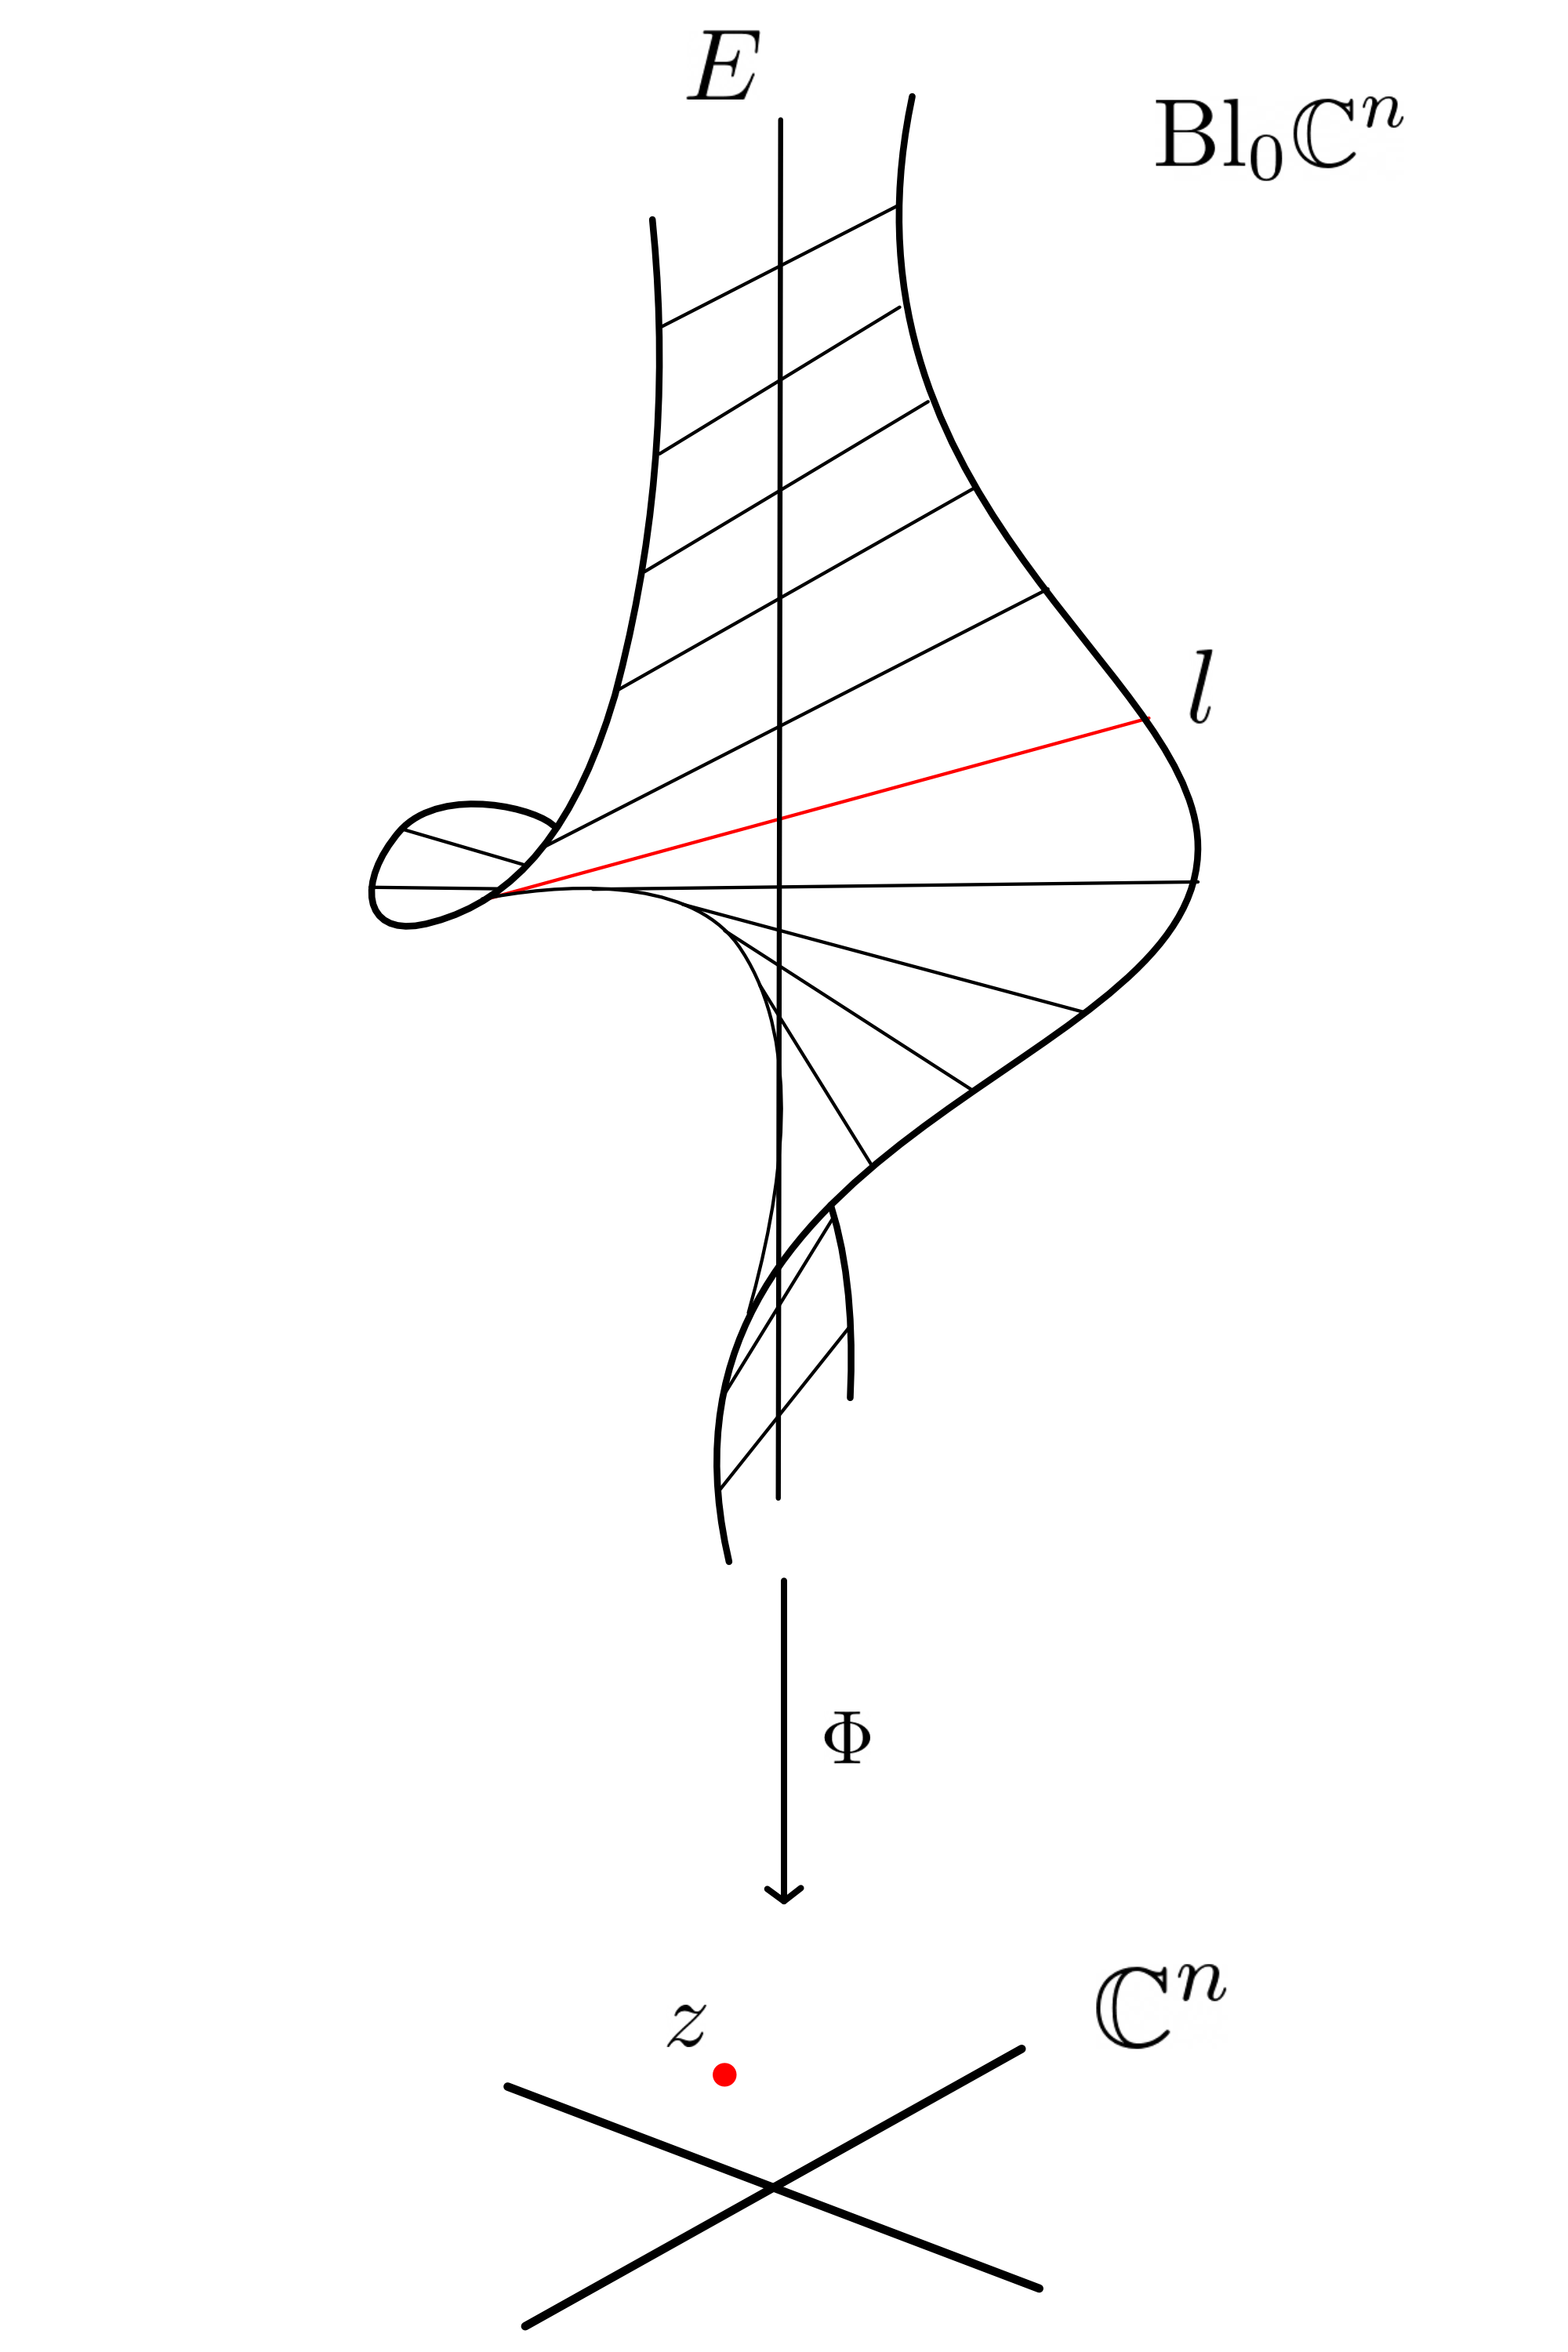
\includegraphics[width=0.45\linewidth]{Imagenes/exposion}
		\caption{Interpretación geométrica del blow-up}
		\label{fig:exposion}
	\end{figure}
	
\end{example}

Las modificaciones son los \enquote{morfismos elementales} de la geometría bimeromorfa, esto debido a que preservan las funciones meromorfas:

\begin{propo}\parencite[Chap VII, Sec. 1, Prop. 1.3]{grauertremment}
	Sea $\Phi:M\to N$ una modificación propia.
	\begin{enumerate}
		\item La aplicación canónica $\widehat{\Phi}:\oo_N\to \Phi_*(\oo_M)$ es un morfismo de gavillas inyectivo.
		\item La aplicación canónica $\widetilde{\Phi}:\mathscr{K}_N\to\Phi_*\mathscr{K}_M$ es un isomorfismo de gavillas.
	\end{enumerate}
	En particular, $\Phi$ induce un isomorfismo de campos $\mathscr{K}(M)\cong\mathscr{K}(N)$.
\end{propo}

\begin{definition}
	Sea $M$ y $N$ variedades complejas. Decimos que una aplicación
	\begin{equation*}
		f:M\dashrightarrow N
	\end{equation*}
	es dice \textbf{meromorfa} si cumple que
	\begin{enumerate}
		\item Existe un subconjunto analítico $A\subset M$ de codimensión al menos $1$ tal que $f$ está bien definido y holomorfo sobre el conjunto abierto denso $U=M\setminus A$. Este conjunto es llamado \textbf{conjunto de indeterminación}.
		\item La cerradura de la gráfica
		\begin{equation*}
			\Gamma_f := \{(x,y)\in U\times N : y=f(x)\}\subset M\times N
		\end{equation*}
		es una subvariedad analítica.
		\item La proyección a la primera coordenada $\Gamma_f\to M$ es una modificación propia.
	\end{enumerate}
	Decimos que $f$ es un \textbf{bimeromorfismo} si existe otra aplicación meromorfa $g:N\dashrightarrow M$ tal que
	\begin{align*}
		f\circ g= id_N,\\
		g\circ f= id_M.
	\end{align*}
	En este caso decimos que $M$ es \textbf{bimeromorfa} a $N$.
\end{definition}

Una aplicación meromorfa $f:M\dashrightarrow N$ puede interpretarse como una aplicación holomorfa después de resolver las indeterminaciones. Específicamente si tomamos las proyecciones
\begin{equation*}
	p_M:\Gamma_f\longrightarrow M\qquad\text{y}\qquad p_N:\Gamma_f\longrightarrow N
\end{equation*}
entonces
\begin{equation*}
	f=p_N\circ p_M^{-1}.
\end{equation*}
Es decir, $f$ se factoriza por una modificación propia. 

De esta manera, $f:N\dashrightarrow M$ es holomorfo casi en todas partes y su gráfica define un subvariedad analítica \enquote{bien comportada} en $M\times N$. La parte \enquote{meromorfa} consiste precisamente en permitir un conjunto de indeterminación de codimensión $\geq 1$, donde no hay una función bien definida.

\begin{remark}\parencite[Chap VII, Sec. 1]{grauertremment}
	Algunos hechos importantes de estas aplicaciones son los siguientes:
	\begin{enumerate}
		\item Si $L$ es un haz lineal sobre $M$, entonces la aplicación inducida
		\begin{equation*}
			\varphi_L:M\longrightarrow\pp^N
		\end{equation*}
		es una aplicación meromorfa, donde el conjunto de indeterminación es $Bs(L)$.
		\item (Teorema de eliminación de indeterminaciones) Sea $f:M\dashrightarrow N$ una aplicación meromorfa. Entonces existe una modificación propia $\sigma:\tilde{M}\to M$ y una aplicación holomorfa $\tau:\tilde{M}\to N$ tal que el siguiente diagrama conmuta
		\begin{center}
			\begin{tikzcd}
				& {\tilde{M}} & \\
				\\
				M && N
				\arrow["\sigma"', from=1-2, to=3-1]
				\arrow["\tau", from=1-2, to=3-3]
				\arrow["f"', from=3-1, to=3-3]
			\end{tikzcd}
		\end{center}
		\item Toda modificación propia es bimeromorfismo.
		\item Toda modificación propia $\Phi:M\to N$ entre superficies complejas compactas es la composición de una cantidad finita de blow-ups en un solo punto.
		\item Toda aplicación bimeromorfa $f:M\dashrightarrow N$ entre variedades complejas compactas puede escribirse como una composición $f=f_1\circ\cdots\circ f_k$ donde $f_i$ son blow-up en un punto o la inversa de un blow-ups en un punto. A la composición de un blow-up con su inversa suele ser llamado \textbf{transformación monoidal}.
	\end{enumerate}
\end{remark}

Análogo al caso de geometría algebraica, si $f:M\dashrightarrow N$ es una aplicación bimeromorfa, entonces induce un isomorfismo de campos
\begin{equation*}
	\mathcal{K}(N)\cong \mathcal{K}(M).
\end{equation*}
Eso significa que
\begin{equation*}
	a(N)=a(M).
\end{equation*}
Por lo tanto, la dimensión algebraica es un invariante bimeromorfo. 

\begin{theorem}[de Moishezon]\parencite{Moishezonlemmachow}
	Sea $M$ una variedad de Moishezon, entonces existe una aplicación bimeromorfa $f:M\dashrightarrow V$ donde $V$ es una variedad algebraica. Es decir, $M$ es bimeromorfa a una variedad algebraica.
\end{theorem}

Este teorema, con un sabor idéntico al \textit{lema de Chow}, muestra una naturaleza algebraica de ciertas variedades complejas. Además, orienta el estudio de la geometría compleja hacia la combinación de técnicas analíticas, birracionales y algebraicas. 

\begin{remark}\parencite[Chap. VII, Sec. 6.4]{grauertremment}\label{espaciosdemoishezon}
	Un \textbf{espacio complejo} (o espacio analítico complejo) es un espacio localmente anillado $(X,\oo_X)$ tal que $X$ es Hausdorff y para cada punto $x\in X$ existe una vecindad $U$ isomorfa a un subconjunto analítico abierto de $\cc^n$, es decir, el espacio localmente anillado $(U,\oo_X|_U)$ es isomorfo a espacio localmente anillado $(Y,\oo_Y)$ donde $Y$ es el abierto
	\begin{equation*}
		Y=\{x\in \Omega\subset\cc^n:f_1(x)=\cdots=f_k(x)=0\}
	\end{equation*}
	junto a la gavilla cociente definida por
	\begin{equation*}
		\oo_Y=\oo_\Omega/\langle f_1,\dots, f_k\rangle,
	\end{equation*}
	restringida a la topología de $Y$.
	
	Los espacios complejos generalizan a las variedades complejas, admitiendo singularidades y elementos nilpotentes en su gavilla. Más aún, existe un funtor llamado \textbf{funtor de analitificación}
	\begin{equation*}
		(\_)^{an}:\{\text{esquemas de tipo finito}/\cc\}\to\{\text{espacios analíticos complejos}\},
	\end{equation*}
	el cual le asocia a un esquema $X$ de tipo finito sobre $\cc$ un espacio complejo $X^{an}$. Sin embargo, este funtor no es una equivalencia pues, como hemos visto, existen muchas variedades complejas (o subconjuntos analíticos en general) que no son algebrizables. Un \textbf{espacio de Moishezon} $X$ es un espacio complejo compacto reducido (sin nilpotentes) bimeromorfo a una variedad algebraica, o equivalentemente,
	\begin{equation*}
		a(X)=\dim X.
	\end{equation*}
	Con lo cual, también hemos trabajado en determinar que espacios de Moishezon sí provienen de esquemas proyectivos de tipo finito sobre $\cc$. Por lo tanto, podemos también preguntarnos: ¿Cuáles son los \enquote{objetos algebraicos} que corresponden con espacios de Moishezon (si es que existen)?
	\end{remark}

\subsection{Variedades de Kähler}

En geometría compleja, la geometría diferencial se desarrolla bajo la restricción impuesta por la estructura compleja. El análogo complejo de una métrica riemanniana es una métrica hermitiana, que es compatible con la estructura compleja y permite introducir nociones métricas respetando la holomorfía. Entre ellas, las métricas de Kähler se distinguen por satisfacer una condición diferencial que unifica la geometría riemanniana, simpléctica y compleja, dando lugar a una teoría especialmente rígida y estructurada.

Para trabajar en este contexto diferencial, primero debemos presentar los espacios tangentes a una variedad compleja. Las construcciones están principalmente basadas de los libros \parencite[Sec. 1.2]{huybrechts2005complex} y \parencite[Cap. 1]{leecomplex}. Fijemos $M$ una variedad compleja y $p\in M$. 
\begin{equation*}
	T_{\rr,p}M=\mathrm{gen}_\rr\left\{\frac{\partial}{\partial x_i},\frac{\partial}{\partial y_i}\right\}.
\end{equation*} 
Definamos el endomorfismo
\begin{align*}
	&J:T_{\rr,p}M\longrightarrow T_{\rr,p}M\\
	J\left(\frac{\partial}{\partial x_i}  \right)&=\frac{\partial}{\partial y_i},\qquad J\left(\frac{\partial}{\partial y_i} \right)=-\frac{\partial}{\partial x_i},
\end{align*}
el cual cumple que $J^2=-\mathrm{Id}$. Esta función es llamada \textbf{estructura casi compleja} de $T_{\rr,p}M$. Ahora, consideremos el espacio complexificado
\begin{equation*}
	T_{\cc.p}M=T_{\rr,p}M\otimes \cc,
\end{equation*}
el cual es llamado \textbf{espacio tangente complejo} de $p$. Además, podemos considerar la extensión de la estructura casi compleja al espacio complexificado $J_\cc:T_{\cc.p}M\to T_{\cc.p}M$. De esta manera, tenemos la descomposición
\begin{equation*}
	T_{\cc.p}M=T_{p}^\prime M\oplus T_p^{\prime\prime}M, 
\end{equation*}
donde
\begin{align*}
	&T_{p}^\prime M=\{v\in T_{\cc.p}M: J(v)=iv\},\\		&T_p^{\prime\prime}M =\{v\in T_{\cc.p}M: J(v)=-iv\}.
\end{align*}
En particular, el espacio $T_{p}^\prime M$ es llamado \textbf{espacio tangente holomorfo} y juega el papel del espacio tangente en la geometría compleja. Además, se cumple que
\begin{equation*}
	\dim_{\cc} T_{p}^\prime M=n
\end{equation*}
pues los operadores 
\begin{equation*}
	\frac{\partial }{\partial z_i}=\frac{1}{2}\left( \frac{\partial }{\partial x_i}-i\frac{\partial }{\partial y_i}\right).
\end{equation*}
forman una base para el espacio tangente holomorfo. Más aún, se tiene la siguiente sucesión exacta de $\rr$-módulos
\begin{center}
	\begin{tikzcd}
		0 & {T_{\mathbb{R},p}M} & {T_{\mathbb{C},p}M} & {T_p^\prime M} & 0
		\arrow[from=1-1, to=1-2]
		\arrow[from=1-2, to=1-3]
		\arrow[from=1-3, to=1-4]
		\arrow[from=1-4, to=1-5]
	\end{tikzcd}
\end{center}
Por lo tanto, podemos concluir que
\begin{equation*}
	T_{\mathbb{R},p}M\cong T_p^\prime M
\end{equation*}
\begin{definition}
	Una \textbf{forma hermitiana} es una función $h:T^\prime_pM\times T^\prime_pM\to\cc$ lineal en la primera entrada y 
	\begin{equation*}
		h(v_1,v_2)=\overline{h(v_2,v_1)},\qquad v_1,v_2\in T^\prime_pM.
	\end{equation*}
\end{definition}
De la definición podemos notar es $\cc$-antilineal y $h_p(v,v)\in\rr$ para todo $v\in T^\prime_pM$. Decimos que $h_p$ es \textbf{positiva definida} si $h_p(v,v)>0$ para todo $v\in T^\prime_pM$.

Usando el isomorfismo $T_{\rr,p}M\cong T^\prime_pM$, podemos ver que si $h_p$ es positivo definido se cumple que
\begin{equation*}
	g(v_1,v_2):=\mathrm{Re}h_p(v_1,v_2)=\frac{1}{2}(h_p(v_1,v_2)+h_p(v_2,v_1))
\end{equation*}
es una métrica riemanniana sobre $M$ como variedad suave. Más aún, $h_p$ está definida únicamente por $g_p$.

\begin{definition}
	Una función bilineal $g:T^\prime_pM\times T^\prime_pM\to\rr$ sobre $M$ se dice \textbf{compatible} con $J$ si
	\begin{equation*}
		g(Ju,Jv)=g(u,v),\qquad\text{para todo }u,v\in T_pM.
	\end{equation*}
\end{definition}

Notemos que la estructura casi compleja $J$ actúa como una rotación $90^\circ$ en cada plano complejo del espacio tangente, pero una métrica albitraria no necesariamente respeta este giro. La compatiblidad de $g$ nos dice que medir después de girar por $J$ es lo mismo que girar después de medir. Un cálculo directo muestra que:
\begin{propo}
	Una función $h_p:T^\prime_pM\times T^\prime_pM\to\cc$ es forma hermitiana si, y solo si, $g_p=\mathrm{Re}h_p$ es una métrica riemanniana en $p$ compatible con $J$.
\end{propo}
%\begin{proof}
%	Supongamos que $h_p:T^\prime_pM\times T^\prime_pM\to\cc$ es una forma hermitiana. Definimos $g:T_{\rr,p}M\times T_{\rr,p}M\to\rr$ la función dada por
%	\begin{equation*}
%		g(v_1,v_2)=\mathrm{Re}h_p(v_1,v_2)=\frac{1}{2}(h_p(v_1,v_2)+h_p(v_2,v_1)).
%	\end{equation*}
%	Notemos que $g$ es bilineal, pues
%	\begin{align*}
%		g(\lambda v_1+v_2,v)=\frac{1}{2}(h_p(\lambda v_1+v_2,v)+h_p(v,\lambda v_1+v_2))=\frac12 (\lambda h_p(v_1,v)+h_p(v_2,v)+\overline{\lambda}\overline{h_p(v_1,v)}´+\overline{h_p(v_1,v)})
%	\end{align*}
%	\textcolor{red}{ACABAR EJEMPLO}
%\end{proof}

Esto significa que la forma hermitiana $h_p$ determina de manera única una métrica riemanniana compatible con $J$, y viceversa. 

Considerando la parte imaginaria
\begin{equation*}
	w_p(u,v)=-\mathrm{Im}h_p(u,v)=\frac{i}{2}(h_p(u,v)-h_p(v,u))
\end{equation*}
es una forma bilineal alternante tal que $w_p(u,v)=g_p(u,Jv)$. Más aún, $h_p$ está definida únicamente por $w_p$.

\begin{propo}
	Una función $h_p:T^\prime_pM\times T^\prime_pM\to\cc$ es forma hermitiana si, y solo si, $w_p=-\mathrm{Im}h_p$ es una 2-forma compatible con $J$.	
\end{propo}
%\begin{proof}
%	\textcolor{red}{FALTA DEMOSTRACIÓN}
%\end{proof}

\begin{definition} 
	Una \textbf{métrica hermitiana} $H$ sobre una variedad compleja $M$ es una colección de formas Hermitianas $h_p$ para todo punto $p\in M$.
\end{definition}

De esta manera, una métrica hermitiana $H$ induce una métrica riemanniana $g=\mathrm{Re}H$ y una $2$-forma diferencial real valuada $w=-\mathrm{Im}H$. A esta forma diferencial se le llamada \textbf{forma fundamental} de $H$. Por lo tanto, esta métrica se puede interpretarse como la versión mínima y natural de una métrica riemanniana que respeta la estructura casi compleja.

\begin{propo}
	Toda variedad compleja admite una métrica hermitiana.
\end{propo}
\begin{proof}
	Sea $M$ una variedad compleja y consideremos una métrica riemanniana $g_0$ arbitraria. Definamos otra métrica riemanniana
	\begin{equation*}
		g(u,v)=g_0(u,v)+g_0(Ju,Jv).
	\end{equation*}  
	Notemos que
	\begin{equation*}
		g(Ju,Jv)=g_0(Ju,Jv)+g_0(J^2u,J^2v)=g_0(-u,-v)+g_0(Ju,Jv)=g_0(u,v)+g_0(Ju,Jv)=g(u,v).
	\end{equation*}
	De esta manera, $g$ es compatible con $J$. Por lo tanto, definiendo $w(u,v)=g(u,Jv)$ obtenemos una métrica hermitiana para $M$
	\begin{equation*}
		h(u,v)=g(u,v)-iw(u,v).
	\end{equation*}
\end{proof}                                     

Si $M$ tiene coordenadas $(z^1,\cdots,z^n)$, entonces una dos forma diferencial $\omega$ está dada por
\begin{equation*}
	\omega=\sum_{i<j}w_{ij}(z)dz^i\wedge dz^j,
\end{equation*}
entonces
\begin{equation*}
	d\omega=\sum_{i<j<k}\left( \frac{\partial w_{jk}}{\partial z_i}+\frac{\partial w_{ki}}{\partial z_j}+\frac{\partial w_{ij}}{\partial z_k}\right)dz^i\wedge dz^j\wedge dz^k.
\end{equation*}
Decimos que $w$ es cerrada si $d\omega=0$.

\begin{definition}
	Una \textbf{variedad de Kähler} es una variedad compleja equipada con una métrica Hermitiana $H$ cuya forma fundamental $\omega=-\mathrm{Im}H$ es cerrada, esto es,
	\begin{equation*}
		d\omega=0.
	\end{equation*}
	En este caso, la forma fundamental $w$ es llamada \textbf{forma de Kähler}.
\end{definition}

La forma fundamental $w$ puede interpretarse como una medida de áreas compatibles con la estructura compleja, por lo que pedir que sea cerrada nos dice que esas áreas complejas no varían infinitesimalmente al moverse en la variedad. Así, la métrica $g$ y la forma $w$ nos respetan los ángulos y áreas a un nivel complejo, es decir, son compatibles con la estructura compleja tanto desde el punto de vista métrico como simpléctico.

Veamos ahora unos ejemplos importantes de variedades de Kähler, los cuales nos ayudarán a entender el caso de algebrización.

\begin{example}
	Consideremos $\cc^n$ con la métrica donde $\frac{\partial}{\partial z_j}$ forman una base unitaria. La estructura casi compleja $J$ actúa sobre los vectores tangentes como
	\begin{equation*}
		J\frac{\partial}{\partial x_j}=\frac{\partial}{\partial y_j},\quad
		J\frac{\partial}{\partial y_j}=-\frac{\partial}{\partial x_j}.
	\end{equation*}
	La métrica euclidiana estándar en $\mathbb{C}^n\simeq\mathbb{R}^{2n}$ es
	\begin{equation*}
		g=\sum_{j=1}^n (dx_j\otimes dx_j+dy_j\otimes dy_j).
	\end{equation*}
	Por otro lado,
	\begin{equation*}
		\omega(u,v)=g(u,Jv).
	\end{equation*}
	En coordenadas, usando que $J$ envía $\partial/\partial x_j\mapsto\partial/\partial y_j$, se obtiene
	\begin{equation*}
		\omega=\sum_{j=1}^n dx_j\wedge dy_j=\frac{i}{2}\sum_{j=1}^{n} dz_i\wedge d\overline{z}_j.
	\end{equation*}
	Como $\omega$ tiene coeficientes constantes, su diferencial exterior es
	\begin{equation*}
		d\omega=\sum_{j=1}^n d(dx_j\wedge dy_j)=
		\sum_{j=1}^n (d dx_j)\wedge dy_j - dx_j\wedge d dy_j=0,
	\end{equation*}
	porque $d (dx_j)=d (dy_j)=0$ para diferenciales exactos de coordenadas. Así que
	\begin{equation*}
		d\omega=0\quad\text{en todo}\qquad \mathbb{C}^n.
	\end{equation*}
	Por lo tanto, $\cc^n$ es una variedad de Kähler.
\end{example}

\begin{example}
	Sea $N\subset M$ una subvariedad compleja. Para todo $p\in N$ se cumple que $T_p^\prime N\subset T_p^\prime M$, entonces una métrica Hermitiana $H_M$ induce naturalmente una métrica en $N$. Calculando en coordenadas locales, se cumple que
	\begin{equation*}
		w_N=i^*w_M
	\end{equation*}
	donde $i:N\hookrightarrow M$ es la aplicación inclusión. Por lo tanto, si $M$ es de Kähler, entonces $N$ también lo es.
\end{example}

\begin{example}[Métrica de Fubini-Study]
	Consideremos el $n$-espacio proyectivo $\pp^n$ y la carta afín
	\begin{equation*}
		U_0=\{[Z_0:\cdots:Z_n]:Z_0\neq 0\}\subset\pp^n.
	\end{equation*}
	con coordenadas locales
	\begin{equation*}
		z_i=\frac{Z_i}{Z_0}.
	\end{equation*} 
	Definamos la función
	\begin{equation*}
		\varphi(z)=\log(1+\|z\|^2)=\log(1+|z_1|^2+\cdots+|z_n|^2).
	\end{equation*}
	llamada \textbf{potencial de Kähler} de la forma 
	\begin{equation*}
		\omega_{FS}=\frac{i}{2\pi}\partial \overline{\partial}\varphi.
	\end{equation*}
	La métrica hermitiana está dada por
	\begin{equation*}
		h_p\left(\frac{\partial}{\partial z_i},\frac{\partial}{\partial z_j}\right)=\frac{\partial^2 \varphi}{\partial z_i\partial \overline{z}_j}=\frac{(1+\|z\|^2)\delta_{ij}-\overline{z}_i z_j}{(1+\|z\|^2)^2}.
	\end{equation*}
	Por las identidades de Dolbeault,
	\begin{equation*}
		\partial^2=\overline{\partial}^2=0,\qquad d=\partial+\overline{\partial}.
	\end{equation*}
	tenemos que
	\begin{equation*}
		d\omega_{FS}=\frac{i}{2\pi}(\partial+\overline{\partial})\partial \overline{\partial}\varphi=\frac{i}{2\pi}(\partial^2\overline{\partial}\varphi+\overline{\partial}\partial\overline{\partial}\varphi)=0.
	\end{equation*}
	Por lo tanto, $\omega_{FS}$ es una forma de Kähler llamada \textbf{forma fundamental de Fubini-Study}.
\end{example}

Como las variedades algebraicas son subvariedades complejas de un espacio proyectivo (véase ejemplo \ref{algsonsubvariedades}), los dos últimos ejemplos implican que todas las variedades algebraicas son variedades de Kähler. Por lo tanto:

\begin{corollary}
	Toda variedad compleja algebrizable es de Kähler.
\end{corollary}

En la teoría de Hodge, se estudia la cohomología de las variedades de Kähler y con una consecuencia de la descomposición de Hodge se llega a la conclusión de que las superficies de Hopf no son de Kähler (véase  \parencite[Corollary 6.13]{2002hodge}). De esta manera, no todas las variedades complejas son de Kähler ni es una condición suficiente para ser algebrizable. 

Una pregunta que nos hicimos en la sección anterior fue ¿Toda variedad de Moishezon es algebrizable? Vimos que si hay algún contraejemplo, debe estar en dimensión $\geq 3$. Vamos a construir el \textit{contraejemplo de Hironaka} que es una variedad de Moishezon de dimensión 3 que no es de Kähler, y en consecuencia tampoco es algebrizable. Para entender este ejemplo, vamos a utilizar un hecho importante de las variedades de Kähler:

\begin{theorem}\label{integralpositiva}
	Sea $M$ una variedad compleja compacta, entonces forma de Kähler $w$ en $M$ se evalúa positivamente sobre cualquier curva compleja irreducible $C\subset M$, es decir,
	\begin{equation*}
		\int_C w>0.
	\end{equation*}
\end{theorem}

\begin{example}[Contraejemplo de Hironoka]\label{hironakaejemplo}\parencite{barlet2015exampleshhironaka}
	Sea $X$ una variedad algebraica no singular de dimensión $3$, por ejemplo podemos tomar $X=\pp^3$. Consideremos dos curvas no singulares $C_1, C_2\subset X$ que se intersectan transversalmente en exactamente dos puntos
	\begin{equation*}
		P,Q\in X.
	\end{equation*} 
	Entonces podemos cubrir a $X$ por dos abiertos
	\begin{equation*}
		X=(X\setminus P)\cup(X\setminus Q).
	\end{equation*}
	Con esto, los puntos $P$ y $Q$ quedan separados por cada abierto. En cada abierto, vamos a hacer dos blow-up: En $X\setminus P$ hacemos un blow-up con centro en $C_1$ y luego hacemos blow-up en la preimagen propia de la curva $C_2$. Análogamente, en $X\setminus Q$ hacemos un blow-up con centro en $C_2$ y luego hacemos blow-up en la preimagen propia de la curva $C_1$.\\
	Como $C_1$ y $C_2$ no se intersectan en $(X\setminus P)\cap(X\setminus Q)$, los dos espacios obtenidos son isomorfos en la intersección y se pueden pegar. Así, obtenemos una variedad compleja $\tilde{X}$ y un bimeromorfismo propio
	\begin{equation*}
		\pi:\tilde{X}\longrightarrow X.
	\end{equation*} 
	Así, $X$ es bimeromorfa a $\tilde{X}$ y $\tilde{X}$ es de Moishezon, pues $X$ lo es. El contraejemplo consiste en demostrar que $\tilde{X}$ no admite métrica de Kähler.\\
	Sea 
	\begin{align*}
		L_1=\pi^{-1}(x),\qquad \text{ con }x\text{ punto genérico de }\enspace C_1.\\
		L_2=\pi^{-1}(y),\qquad \text{ con }y\text{ punto genérico de }\enspace C_2.
	\end{align*}
	Entonces
	\begin{equation*}
		L_1\cong \pp^1,\qquad L_2\cong\pp^1,
	\end{equation*}
	pues son fibras excepcionales de blow-up de curvas en una $3$-variedad. Ahora, la fibra de $\pi$ en $Q$ se descompone en dos componentes irreducibles
	\begin{equation*}
		\pi^{-1}(Q)=L_1^\prime\cup L_2^\prime,
	\end{equation*}
	donde $L_1^\prime$ proviene del blow-up a lo largo de $C_1$ y $L_2^\prime$ proviene del blow-up a lo largo de $C_2$. Además, se tienen las siguientes relaciones homológicas
	\begin{align*}
		&L_1^\prime\sim L_1\\
		&L_2^\prime\sim L_2\\
		&L_1^\prime+L_2^\prime\sim L_1
	\end{align*}
	Análogamente en $P$ obtenemos la descomposición $\pi^{-1}(P)=L_1^{\prime\prime}\cup L_2^{\prime\prime}$ con las relaciones
	\begin{align*}
		&L_1^{\prime\prime}\sim L_1\\
		&L_2^{\prime\prime}\sim L_2\\
		&L_1^{\prime\prime}+L_2^{\prime\prime}\sim L_2
	\end{align*}
	Así, obtenemos que
	\begin{equation*}
		L_1^\prime+	L_2^\prime\sim 0\qquad\text{en}\enspace H_2(\tilde{X},\zz).
	\end{equation*}	
	Si $\tilde{X}$ admitiera una forma de Kähler $w$, entonces por el teorema \ref{integralpositiva} tendríamos que
	\begin{equation*}
		\int_{L^\prime_1} w >0,\qquad	\int_{L^\prime_2} w >0.
	\end{equation*}
	Luego
	\begin{equation*}
		\int_{L^\prime_1+L^\prime_2} w>0.
	\end{equation*}
	Sin embargo, como el ciclo $L_1^\prime+	L_2^\prime$ es homológicamente trivial entonces $\int_{L_1^\prime+L_2^\prime}w=0$, lo cual es una contradicción. Por lo tanto, $\tilde{X}$ no admite métricas de Kähler. En consecuencia, $\tilde{X}$ tampoco puede ser algebrizable.
	\begin{figure}[H]
		\centering
		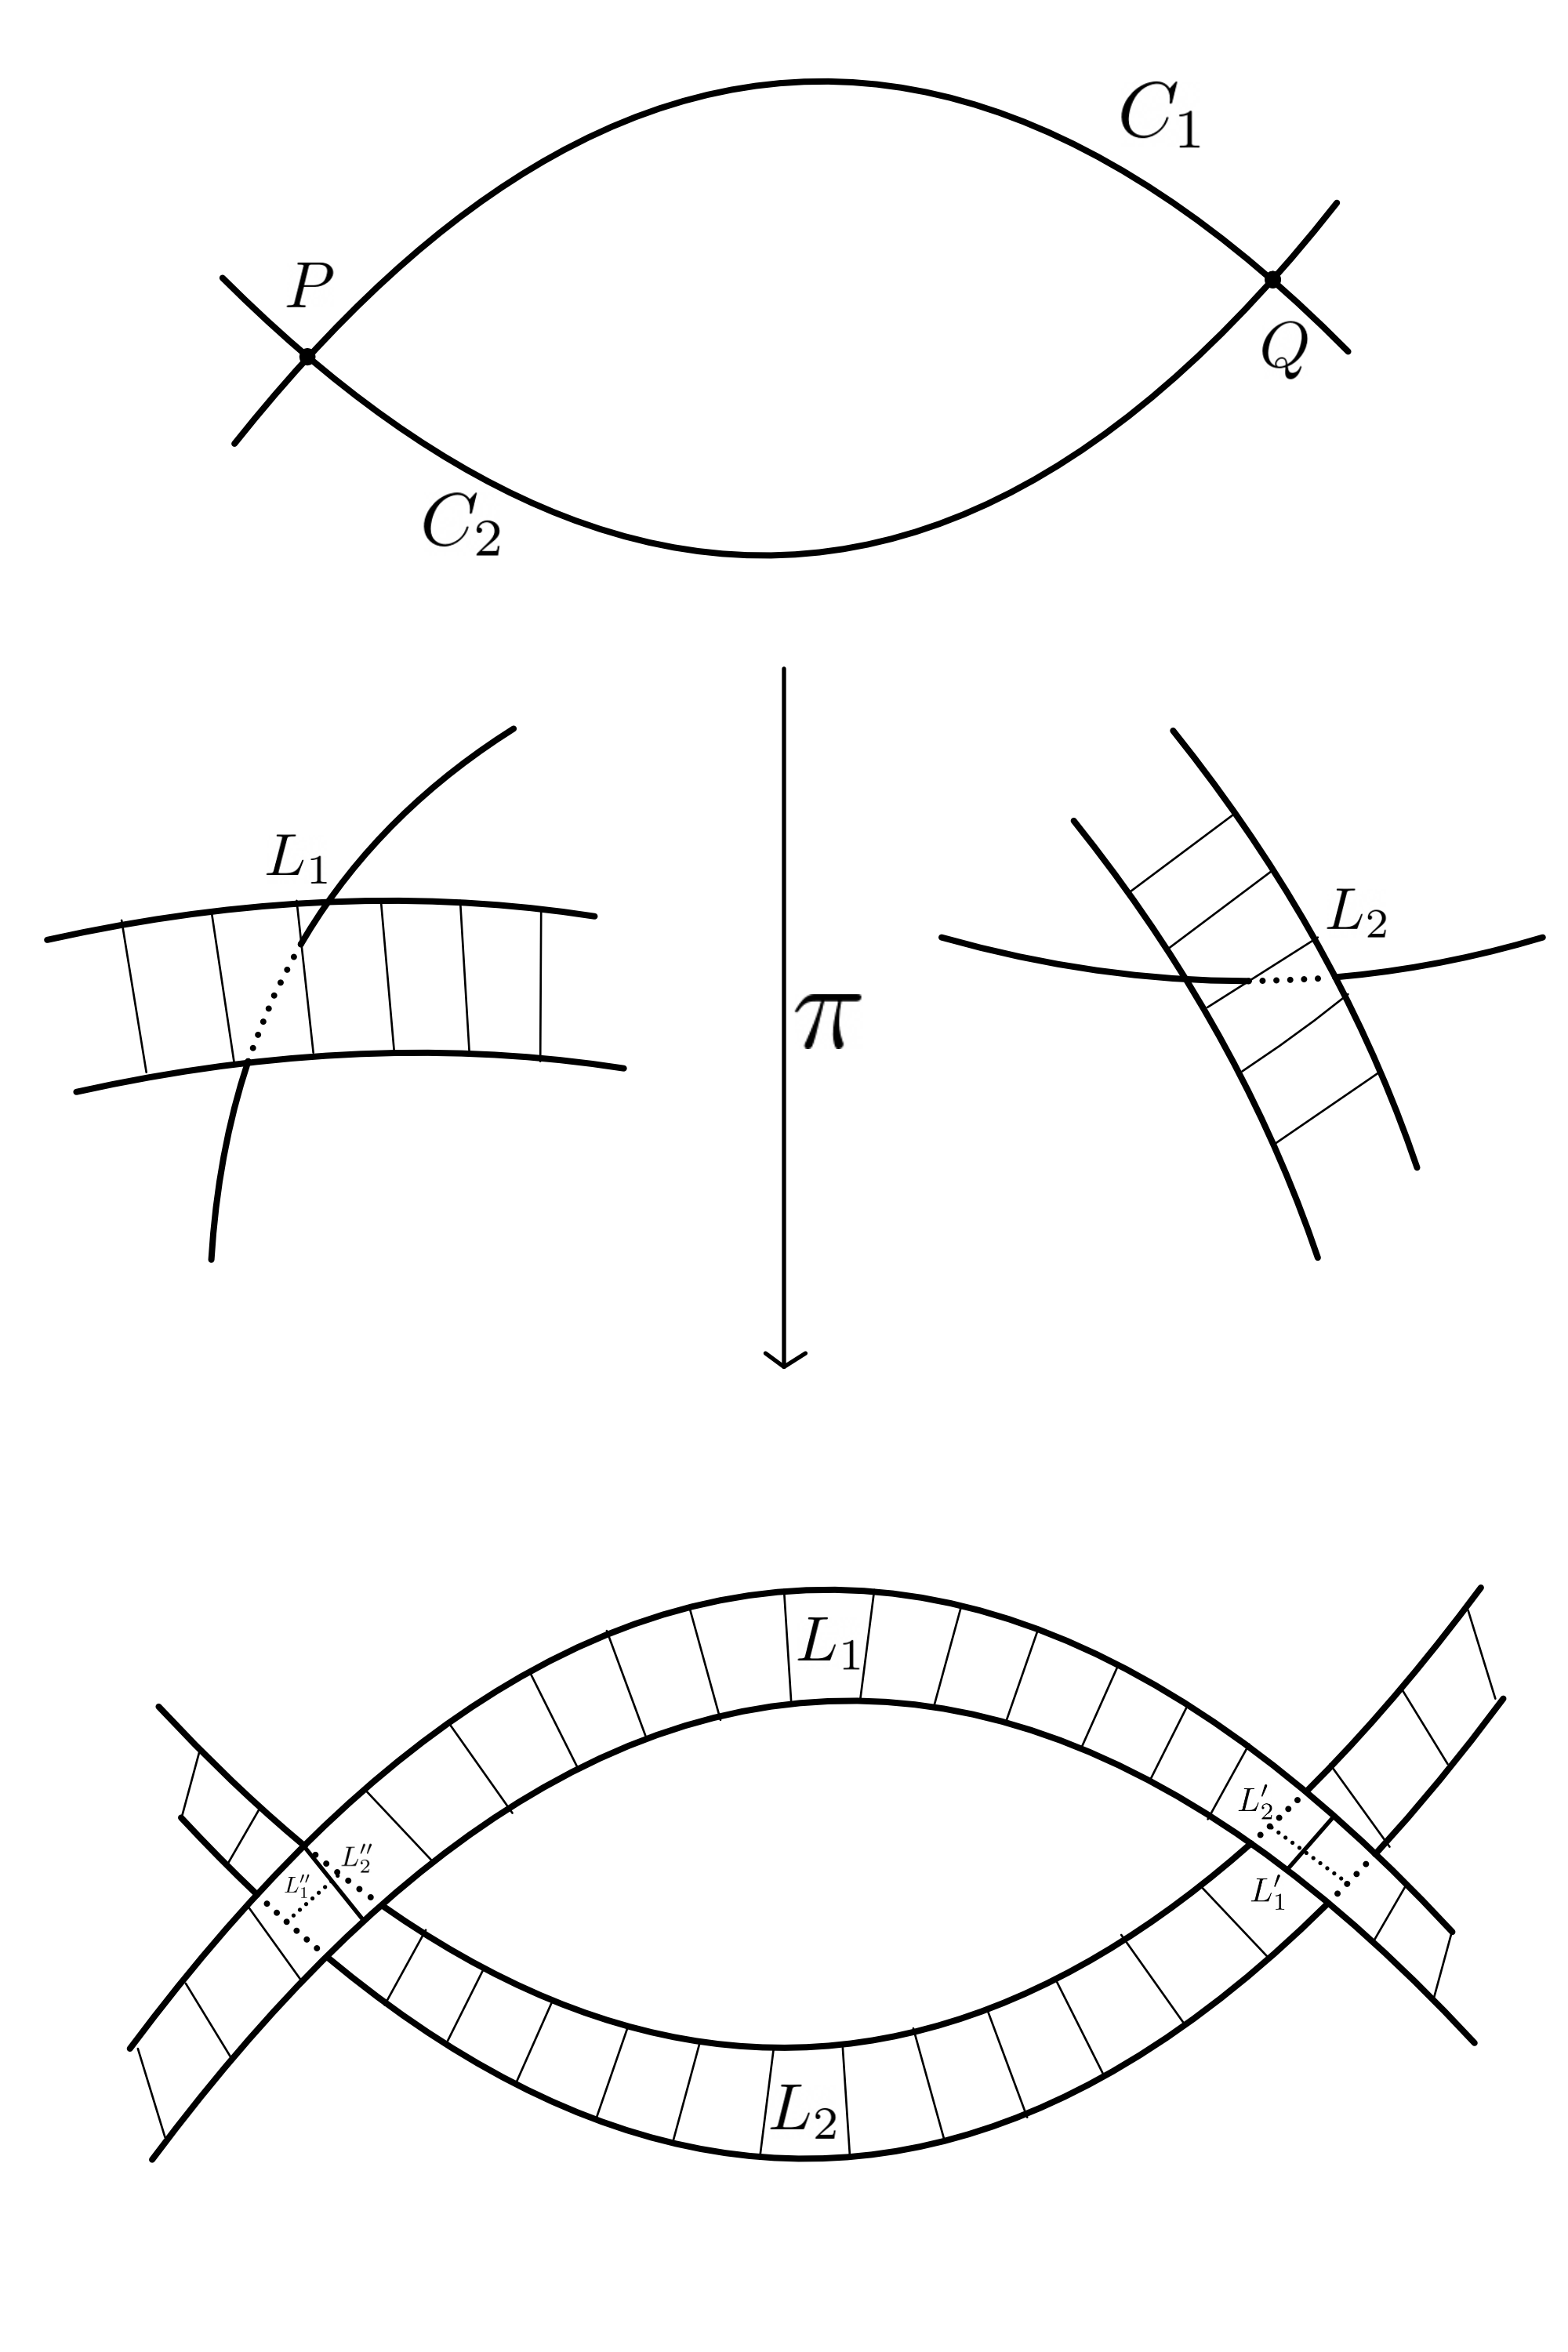
\includegraphics[width=0.4\linewidth]{Imagenes/Ejemplo Hironaka}
		\caption{Contraejemplo de Hironaka}
		\label{fig:ejemplo-hironaka}
	\end{figure}
\end{example}

\begin{remark}\parencite[Chap. VII, Sec. 6.4]{grauertremment}
	Continuando la observación \ref{espaciosdemoishezon}. El matemático americano \textit{Michael Artin} desarrolló unos objetos llamados \textbf{espacios algebraicos}. Intuitivamente, en lugar de utilizar esquemas afines como piezas locales de esquemas, los puntos en un espacio algebraico solo tienen vecindades étale y estas \enquote{piezas étale} luego deben pegarse. Los esquemas son naturalmente espacio algebraicos, pero una observación importante es que el contraejemplo de Hironaka genera un espacio algebraico que no es esquema. Además, se puede extender el funtor de analitificación al funtor
	\begin{equation*}
		(\_)^{an}:\{\text{espacios algebraicos de tipo finito }/\cc\}\longrightarrow\{\text{espacios complejos}\}.
	\end{equation*}
	En particular, Artin probó que este funtor induce la equivalencia categórica
	\begin{equation*}
		\{\text{espacios algebraicos propios de tipo finito}/\cc\}\cong\{\text{espacios de Moishezon}\}.
	\end{equation*}
	En otras palabras, todo espacio de Moishezon es de manera única un espacio algebraico, es decir, los espacios de Moishezon no se pueden pegar en general con la topología de Zariski como los esquemas, pero sí con la topología étale. Concluyendo que, para las necesidades de la geometría bimeromorfa, la categoría de esquemas suele ser insuficiente pues hay muy pocos objetos. Pero la categoría de espacios algebraicos sí lo es: no se puede abandonar esta categoría mediante modificaciones. 
\end{remark}

El resultado más importante de esta sección y conclusión final es el otro teorema demostrado por Moishezon.

\begin{theorem}[Teorema fundamental de Moishezon]\parencite{Moishezon1967}\label{fundamentaldemoishezon}
	Toda variedad de Moishezon y Kähler es algebrizable.
\end{theorem}

Este resultado conecta de forma conclusiva las distintas áreas de la geometría, pues significa que condiciones algebraicas y diferenciables en un contexto complejo imponen una estructura algebraica. De este modo, el teorema nos muestra la interacción entre la geometría diferencial, a través de la existencia de métricas de Kähler, y la geometría algebraica mediante la dimensión algebraica, dentro del marco de la geometría compleja, concluyen de manera natural al problema de algebrización abordado durante todo este trabajo. 

	
	
	%-----------------------new page----------------------------
	
%	\chapter{Encaje al proyectivo}\label{cap2}

	Encajar variedades en otros espacios juega un papel importante en la geometría diferencial, pues permiten trabajar variedades muy abstractas como subvariedades de algún espacio ya conocidos. Existen varios resultados clásicos en esta dirección, por ejemplo:
	
    \begin{theorem}[Teorema del Encaje de Whitney]
        Toda variedad diferenciable suave de dimensión $n$ admite un encaje suave y propio a $\rr^{2n+1}$.
    \end{theorem}
    
    Aunque este resultado no siempre proporciona la mejor cota posible para la dimensión del espacio ambiente\footnote{En general, $2n$ es suficiente para un encaje suave, pero es más complicado de probar. Además, una superficie real orientable puede encajarse en $\rr^3$, mientras que una no orientable puede encajarse, en general, en $\rr^4$.}, su importancia conceptual es fundamental, pues permite considerar toda variedad suave real como un objeto concreto dentro de algún espacio euclidiano $\rr^N$. Esta perspectiva hace posible abordar numerosas cuestiones geométricas y topológicas mediante herramientas del cálculo y de la geometría clásica \parencite[Ver Cap.~6]{lee2003smooth}.
    
    En el contexto de la geometría compleja la situación es sustancialmente más restrictiva (véase el ejemplo \ref{encajeccn}). La inexistencia general de un teorema de encaje holomorfo en espacios afines complejos podría parecer, en principio, una limitación.
    
    No obstante, conviene recordar uno de los ejemplos fundamentales de variedades complejas: las variedades algebraicas. Estas son variedades complejas que se realizan de manera natural como subvariedades del espacio proyectivo complejo. Dicho espacio ambiente posee propiedades topológicas y algebraicas de gran relevancia, como la topología de Zariski y la compacidad, que resultan extremadamente útiles desde el punto de vista geométrico.
   
    \begin{example}
        Consideremos el polinomio $f(x,y)=y^2-x^3+x\in\cc[x,y]$, el cual tiene grado $3$, es irreducible y no singular. Entonces 
        \begin{equation*}
            Z(f)=\{(x,y)\in\mathbb{C}^2: f(x,y)=0\}
        \end{equation*}
        es una curva compleja.
        \begin{figure}[H]
        	\centering
        	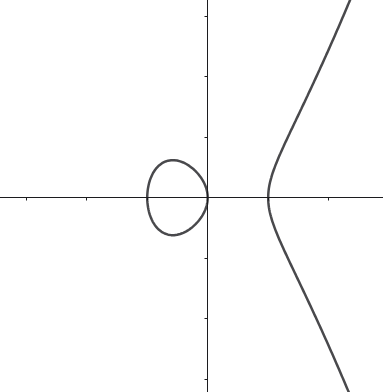
\includegraphics[width=0.25\linewidth]{Imagenes/Curva eliptica afin}
        	\caption{Curva algebraica afín $Z(y^2-x^3+x)$.}
        	\label{fig:curva-eliptica-afin}
        \end{figure}
        Ahora consideremos la homogeneización del polinomio $f(x,y)$ dada por
        \begin{equation*}
            F(X,Y,Z)=Z^3\left( \left(\frac{Y}{Z}\right)^2-\left(\frac{X}{Z}\right)^3+\frac{X}{Z}\right)=Y^2Z-X^3+XZ^2\in\cc[X,Y,Z].
        \end{equation*}
        Este polinomio es homogéneo de grado $3$ y su conjunto de ceros
        \begin{equation*}
            X=Z(F)=\{[X:Y:Z]\in\pp^2:F(X,Y,Z)=0\}
        \end{equation*}
        es una curva algebraica proyectiva. Ahora estudiemos sus puntos al infinito.\\
        Si $Z=0$, entonces $-X^3=0$. Esto implica que $X=0$. Por lo que el único punto al infinito es 
        \begin{equation*}
            [0:1:0].
        \end{equation*}
        Queremos ver ahora que $F$ no es singular en $[0:1:0]$. Las parciales de $F$ están dadas por
        \begin{equation*}
            F_X=-3X^2+Z^2,\qquad F_Y=2XZ,\qquad F_Z=Y^2+2XZ.
        \end{equation*}
        Con lo que, evaluando en el punto $[0:1:0]$, tenemos que
        \begin{equation*}
            F_X(0,1,0)=0,\qquad F_Y(0,1,0)=0,\qquad F_Z(0,1,0)=1.
        \end{equation*}
        Como no todas las parciales son cero, la curva es no singular en ese punto. Como $X$ es una curva proyectiva no singular, posee estructura natural de superficie de Riemann. Además, la fórmula de Plücker nos muestra que tiene género 1. (véase figura \ref{fig:toro}).
        
        Más aún, dado que $X\subset\pp^2$ entonces $X$ es una variedad compleja que vive dentro del plano proyectivo $\pp^2$. Más adelante veremos que, de hecho, es una subvariedad compleja y subvariedad analítica de $\pp^2$.
    \end{example}
    
    Considerando el caso de las variedades algebraicas proyectivas, surge de manera natural la siguiente pregunta: \textit{¿Qué variedades complejas pueden realizarse como subvariedades de algún espacio proyectivo complejo?} Tan sencilla como aparentemente específica, esta pregunta constituye la motivación central de este trabajo. Su respuesta, sin embargo, dista de ser inmediata y conduce a resultados considerablemente más profundos de lo que su formulación inicial pueda sugerir.
    
\section{Encaje Holomorfo}
	
	Antes de responder la pregunta anterior, introduciremos las nociones necesarias para formular con precisión el problema.
	
	Un \textit{encaje holomorfo} es una aplicación holomorfa que preserva la estructura compleja, la topología y la geometría exterior de una variedad compleja. El estudio de estos encajes nos revela profundas interacciones entre la geometría compleja, la teoría de haces y la cohomología, y nos conduce de manera natural a problemas centrales como la algebraización de variedades complejas y su relación con espacios proyectivos. En esta sección vamos A introducir el concepto de encaje holomorfo para analizar sus propiedades básicas, así como algunos ejemplos y contraejemplos relevantes.
	    
    \begin{definition}
        Sean $M$ y $N$ variedades complejas de dimensión $n$ y $k$ respectivamente. Una aplicación holomorfa $f:N\to M$ es un \textbf{encaje holomorfo} si satisface:
        \begin{enumerate}
            \item $f$ es inyectiva.
            \item (\textbf{Encaje topológico}) $f$ es un homeomorfismo con su imagen, es decir, $f:N\to f(N)$ es biyectiva, continua y con inversa continua ($f(N)$ lleva la topología del subespacio de $M$).
            \item Para cada $p\in N$, existen cartas $(U,\varphi)$ alrededor de $f(p)\in M$ y $(V,\psi)$ alrededor de $p\in N$ tales que $f(V)\subset U$ y en coordenadas
            \begin{equation*}
                \varphi\circ f\circ\psi^{-1}(z_1,\cdots,z_k)=(z_1,\cdots,z_k,0\cdots,0)\in\cc^n.
            \end{equation*}.
        \end{enumerate}
        Notemos que la condición $3$ nos indica que $f$, localmente, coincide con la inclusión $\cc^k\hookrightarrow\cc^n$, $z\mapsto (z,0)$.
    \end{definition}

    \begin{example}[Gráfica de una aplicación holomorfa]
    	Sea $N$ una variedad compleja de dimensión $n$ y $g:N\to\cc^{m}$ una aplicación holomorfa. Consideremos la aplicación
    	\begin{align*}
    		f:N\longrightarrow N\times\cc^{m}\\
    		z\mapsto(z,g(z)).
    	\end{align*}
    	Notemos que $f$ es una aplicación holomorfa pues cada una de sus componentes es holomorfa. Además, es inyectiva pues es la identidad en la primera entrada.\\
    	Luego, la aplicación inversa $f^{-1}:f(N)\to N$ está dada por
    	\begin{equation*}
    		f^{-1}(z,g(z))=z
    	\end{equation*}
    	la cual es continua. Por lo que $f:N\to f(N)$ es un homeomorfismo.\\ 
    	Consideremos una carta $(U,\varphi)$ una carta de $N$, $\varphi:U\to V\subset\cc^n$. Definamos la aplicación holomorfa $G:=g\circ \varphi^{-1}:V\to\cc^m$. De esta manera, obtenemos el biholomorfismo 
    	\begin{align*}
    		\Psi:V\times \cc^m\longrightarrow V\times \cc^m\\
    		(z,w)\mapsto (z,w-G(z)),
    	\end{align*}
    	pues su inversa es la aplicación $(z,w)\mapsto (z,w+G(z))$. Con lo cual, 
    	\begin{equation*}
    		\Psi(\varphi(U)\times\cc^m\cap f(U))=\{(z,0):z\in V\cap\varphi(U)\}=V\times\{0\}.
    	\end{equation*}
    	Definamos entonces la carta $\psi=\Psi\circ (\varphi\times \text{id})$ se cumple que
    	\begin{equation*}
    		\psi\circ f\circ \varphi^{-1}:V\to V\times\cc^m\subset \cc^{n+m} 
    	\end{equation*}
    	está dada por
    	\begin{equation*}
    		\psi\circ f\circ\varphi^{-1}(z)=(z,0)\in\cc^n\times\cc^m.
    	\end{equation*}
    	Por lo tanto, se cumple la definición de encaje holomorfo.\\
        Intuitivamente, $f$ está \enquote{dibujando} a la variedad $N$ dentro de $N\times\cc^m$ sin doblarla y sin autointersectarla.
        \begin{figure}[H]
        	\centering
        	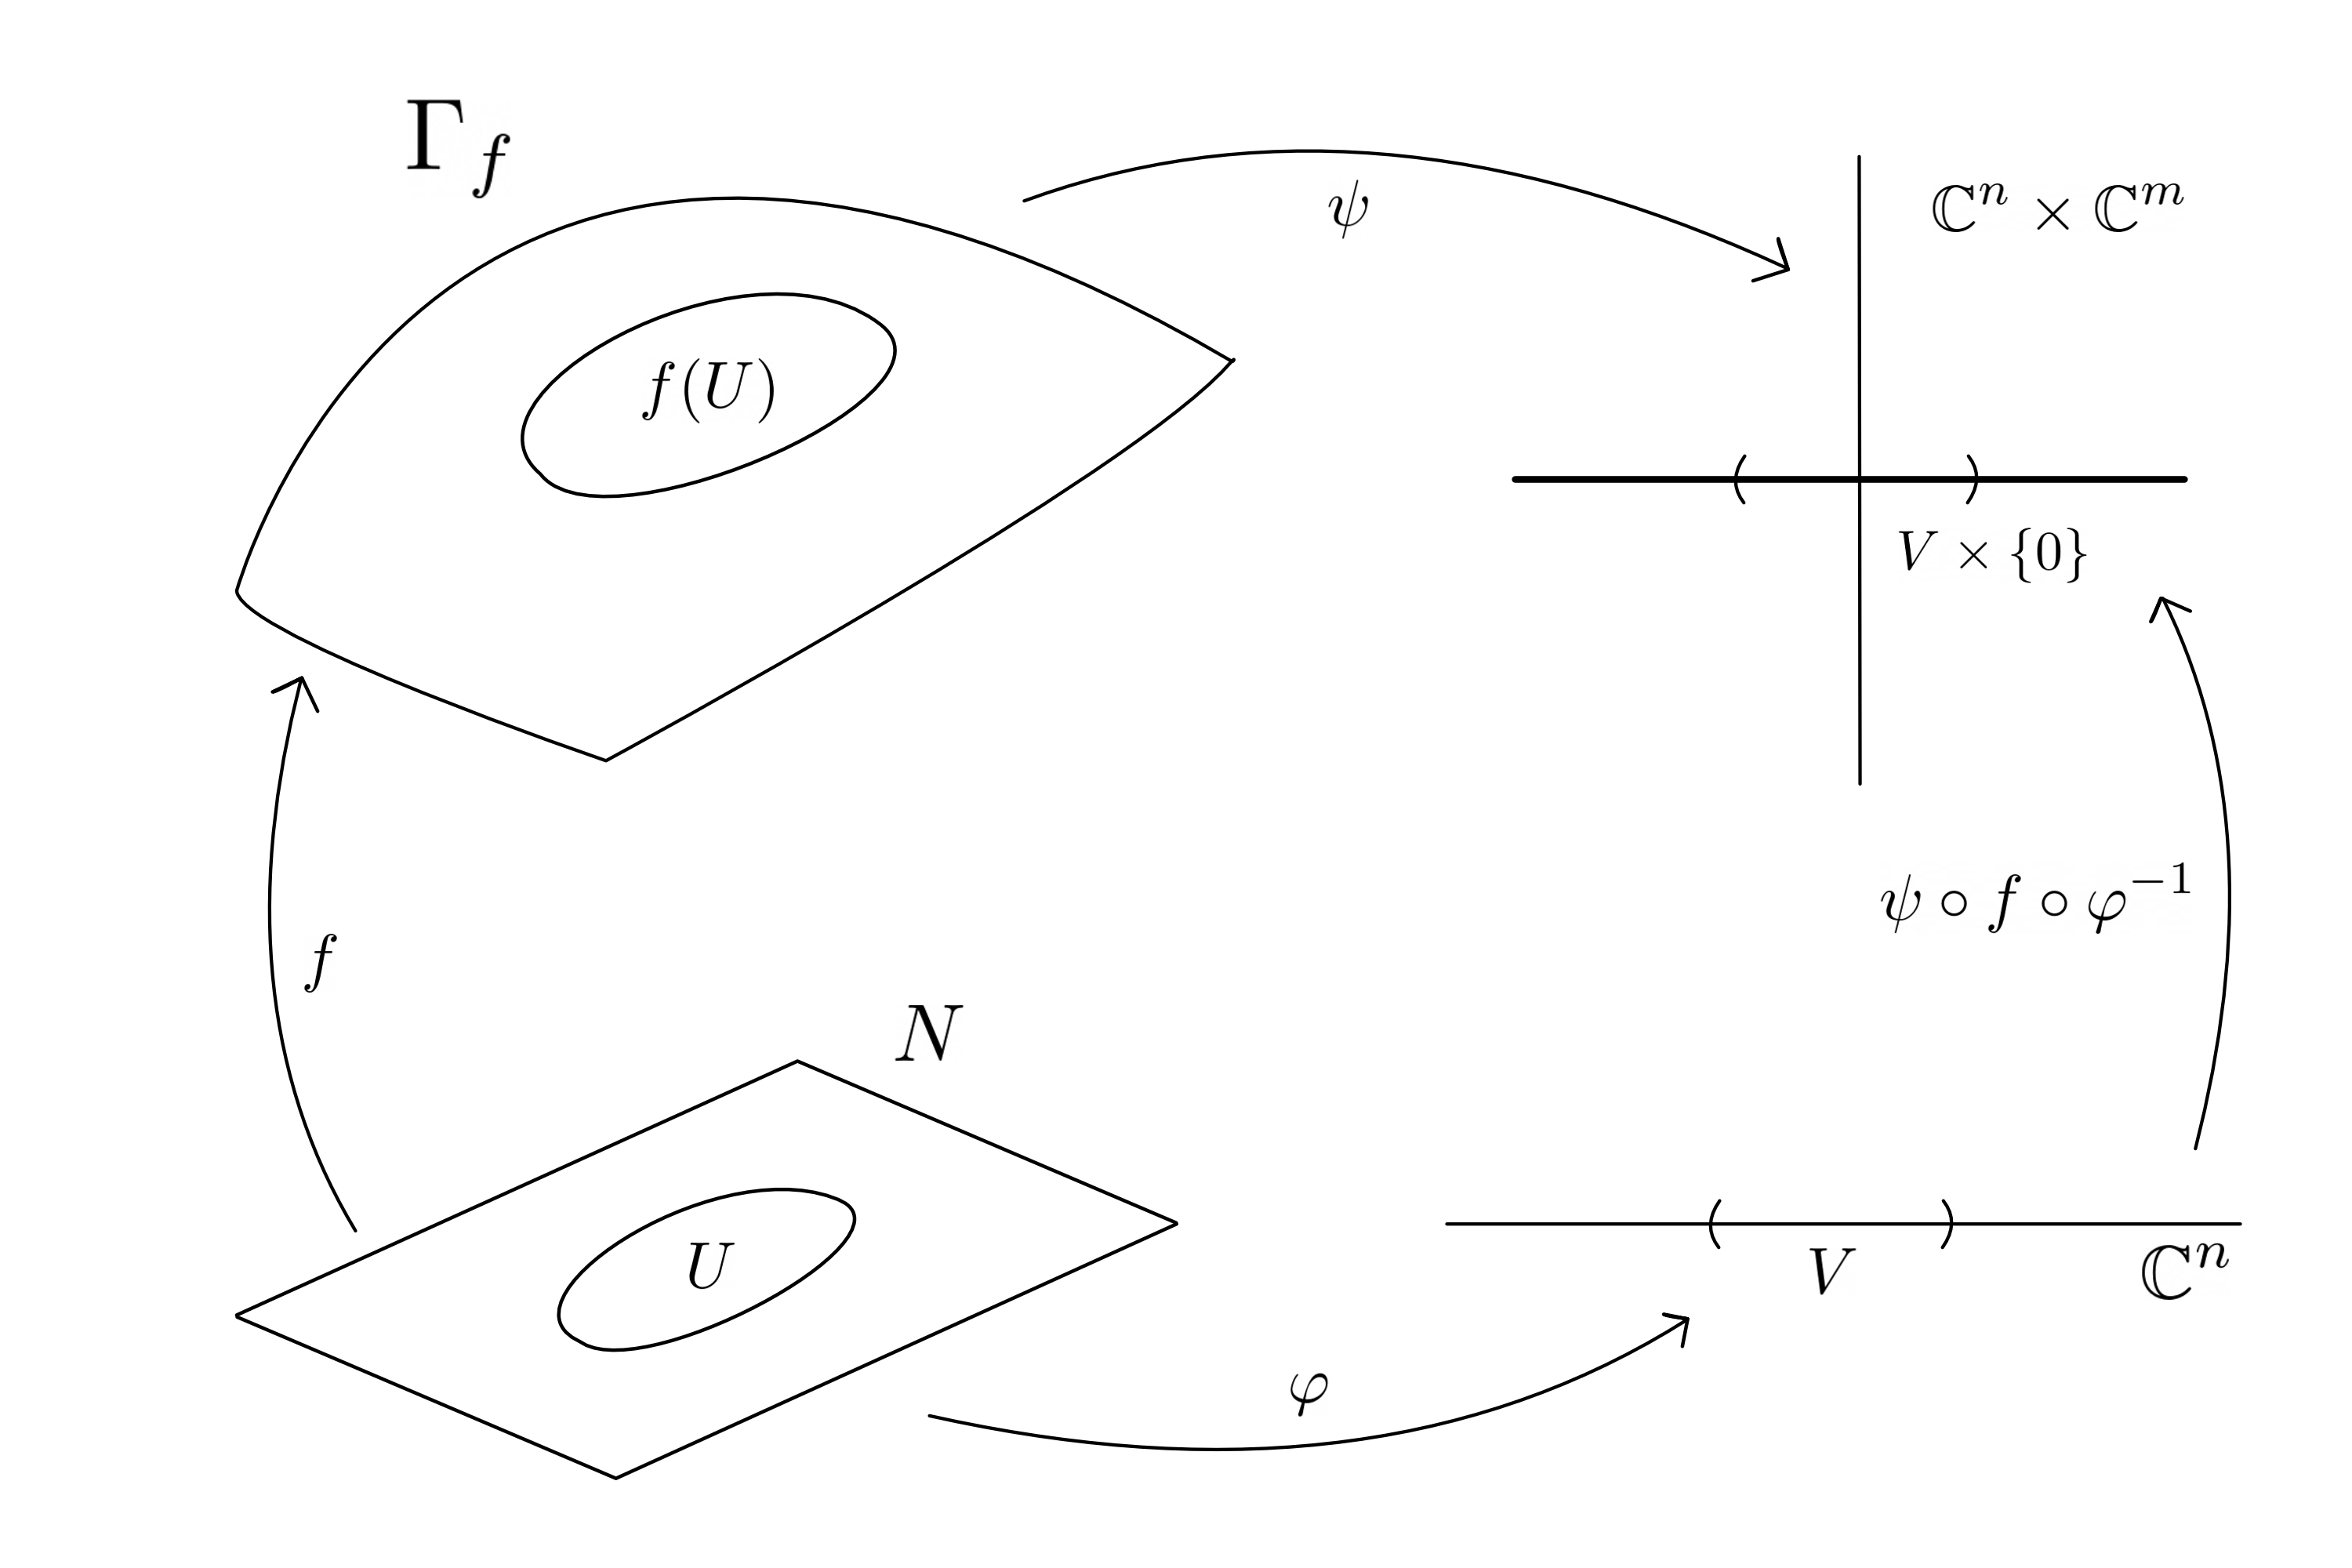
\includegraphics[width=0.6\linewidth]{Imagenes/Encaje de grafica}
        	\caption{Diagrama del encaje dada por una aplicación holomorfa.}
        	\label{fig:encaje-de-grafica}
        \end{figure}
         
    \end{example}
    
    
    \begin{definition}[Subvariedad compleja]
        Una variedad compleja $N$ es una subvariedad compleja (de dimensión $k$) de una variedad compleja $M$, con $\dim M=n$, si $N\subset M$ y existe un atlas holomorfo $\{U_i,\varphi_i\}$ de $M$ tal que 
        \begin{equation*}
            \varphi_i(U_i\cap N)\cong \varphi_i(U_i)\cap\cc^k
        \end{equation*}
        donde $\cc^k$ está encajado en $\cc^n$ por $z\mapsto (z,0)$. Definimos la \textbf{codimensión} de $N$ en $M$ como
        \begin{equation*}
            \mathrm{codim}N:=\dim M-\dim N=n-k.
        \end{equation*}
    \end{definition}
    
    \begin{remark}\label{subvariedadesporecuaciones} $ $
    	\begin{enumerate}
    		\item Si $N$ es una subvariedad compleja de $M$, entonces la inclusión $i:N\hookrightarrow M$ es un encaje holomorfo. Más aún, si $f:N\to M$ es un encaje holomorfo, entonces $f(N)$ es una subvariedad compleja de $M$.
    		\item Consideremos una variedad compleja $M$ y una subvariedad compleja $N\subset M$ de dimensión $k$. Por definición, para todo punto $p\in N$ existe una carta holomorfa $(U,\varphi)$ de $M$ tal que, después de identificar $\cc^k$ con el subespacio lineal
    		\begin{equation*}
    			\cc^k\times\{0\}\subset\cc^n
    		\end{equation*}
    		se cumple que
    		\begin{equation*}
    			\varphi(U\cap N)=\varphi(U)\cap (\cc^k\times \{0\}).
    		\end{equation*}
    		Si tomamos las coordenadas $z_1,\dots,z_n$ de $\cc^n$, entonces en dicha carta, $U\cap N$ queda descrita por las ecuaciones 
    		\begin{equation*}
    			z_{k+1}=\cdots=z_n=0.
    		\end{equation*}
    		Equivalentemente
    		\begin{equation*}
    			U\cap N=\bigcap_{j=k+1}^n f_j^{-1}(0)=Z(f_{k+1},\dots f_n),
    		\end{equation*}
    		donde $f_j=z_j\circ \varphi$. Por lo tanto, localmente $N$ es una subvariedad de intersección completa descrita por $n-k$ funciones holomorfas.
    	\end{enumerate}
    \end{remark}

	\begin{example}\label{algsonsubvariedades}
		Toda variedad algebraica no singular es una subvariedad compleja del espacio proyectivo. 
			Sea $V\subset\pp^n$ una variedad algebraica proyectiva no singular. Por definición, existe una cantidad finita de polinomios homogéneos $F_1,\dots,F_r\in \cc[x_0,\dots,x_n]$ tal que
			\begin{equation*}
				V=Z(F_1,\dots,F_r).
			\end{equation*}
			Fijemos una carta afín $U_i\subset \pp^n$
			y consideremos las coordenadas afines
			\begin{equation*}
				z_j=\frac{x_j}{x_i},\qquad j\neq i.
			\end{equation*}
			En esta carta, las ecuaciones homogéneas se transforman en ecuaciones polinómicas
			\begin{equation*}
				f_\ell(z_1,\dots,\widehat{z_i},\dots,z_n)=0,
				\qquad \ell=1,\dots,r,
			\end{equation*}
			donde cada $f_\ell$ es una función holomorfa sobre $U_i\cong \cc^n$. De esta manera,
			\begin{equation*}
				V\cap U_i=\{p\in U_i : f_1(p)=\cdots=f_r(p)=0\}
			\end{equation*}
			Sea $p\in V\cap U_i$. Como $V$ es no singular, el jacobiano de las ecuaciones tiene rango máximo igual a la codimensión de $V$ en $\pp^n$. Por el teorema de la función implícita \ref{funcionimplicita}, existen coordenadas holomorfas locales
			\begin{equation*}
				(w_1,\dots,w_n)
			\end{equation*}
			en una vecindad de $p$ tales que
			\begin{equation*}
			 V\cap U_i=Z(w_{k+1},\dots w_n).
			\end{equation*}
			Por lo observación \ref{subvariedadesporecuaciones}, $V$ es una subvariedad compleja de $\pp^n$, y la estructura compleja inducida coincide con la obtenida mediante las cartas holomorfas de $\pp^n$.
	\end{example}

	\begin{example}[Biholomorfismo que no es encaje]
		Sea $f:\cc\to\cc^*\times\cc^*$ la aplicación holomorfa
		\begin{equation*}
			f(z)=(e^z,e^{\alpha z}),
		\end{equation*}
		donde $\alpha\in\rr\setminus\mathbb{Q}$. Vamos a probar que $f$ es biholomorfa a su imagen. 
		
		Para la inyectividad, supongamos que $f(z)=f(w)$. Entonces
		\begin{equation*}
			e^{z-w}=1,\qquad e^{\alpha(z-w)}=1.
		\end{equation*}
		Así, existen $n,m\in \zz$ tales que
		\begin{equation*}
			z-w=2\pi i n,\qquad \alpha(z-w)=2\pi im.
		\end{equation*}
		Si $n\neq 0$, entonces $\alpha=m/n\in\mathbb{Q}$ lo cual es una contradicción. De esta manera, $n=0$ e implica que $z=w$. Por tanto, $f$ es inyectiva.
		
		Fijemos $z_0\in\cc$ y pongamos
		\begin{equation*}
			p=f(z_0).
		\end{equation*}
		Como la primera coordenada de $p=(p_1,p_2)$ es un punto en $\cc^*$, existe una vecindad $V$ de $p_1=e^{z_0}$ donde existe una rama del logaritmo
		\begin{equation*}
			\log_V:V\longrightarrow\cc.
		\end{equation*}
		Entonces, en una vecindad suficientemente pequeña de $p$ dentro de la imagen
		\begin{equation*}
			f^{-1}(w_1,w_2)=\log_V(w_1).
		\end{equation*}
		Con esto, $f^{-1}$ es holomorfa alrededor de cada punto de la imagen. Es decir, la aplicación
		\begin{equation*}
			f^{-1}:f(\cc)\longrightarrow\cc
		\end{equation*}
		es holomorfa. Con esto, $f$ es biholomorfa con su imagen. 
		
		Para probar que $f$ no es encaje, vamos a probar que $f:\cc\to f(\cc)$ no es un homeomorfismo si $f(\cc)$ lleva la topología del subespacio. 
		
		Consideremos la sucesión 
		\begin{equation*}
			z_n=2\pi in.
		\end{equation*} 
		Entonces
		\begin{equation*}
			f(z_n)=(1,e^{2\pi i\alpha n}).
		\end{equation*}
		Como $\alpha$ es irracional, la sucesión $\{e^{2\pi i\alpha n}\}$ es densa en $S^1$. Por lo que, existe una subsucesión $n_k$ tal que
		\begin{equation*}
			e^{2\pi i\alpha n_k}\longrightarrow 1.
		\end{equation*} 
		De esta manera, 
		\begin{equation*}
			f(z_{n_k})\longrightarrow (1,1)=f(0).
		\end{equation*}
		Sin embargo, $z_{n_k}=2\pi i n_k$ no converge a $0\in\cc$. Por lo que, la inversa $f^{-1}:f(\cc)\to\cc$ no es continua como espacios métricos, es decir, $f:\cc\to f(\cc)$ no es un homeomorfismo con la topología del subespacio de $f(\cc)$.
		\begin{figure}[H]
			\centering
			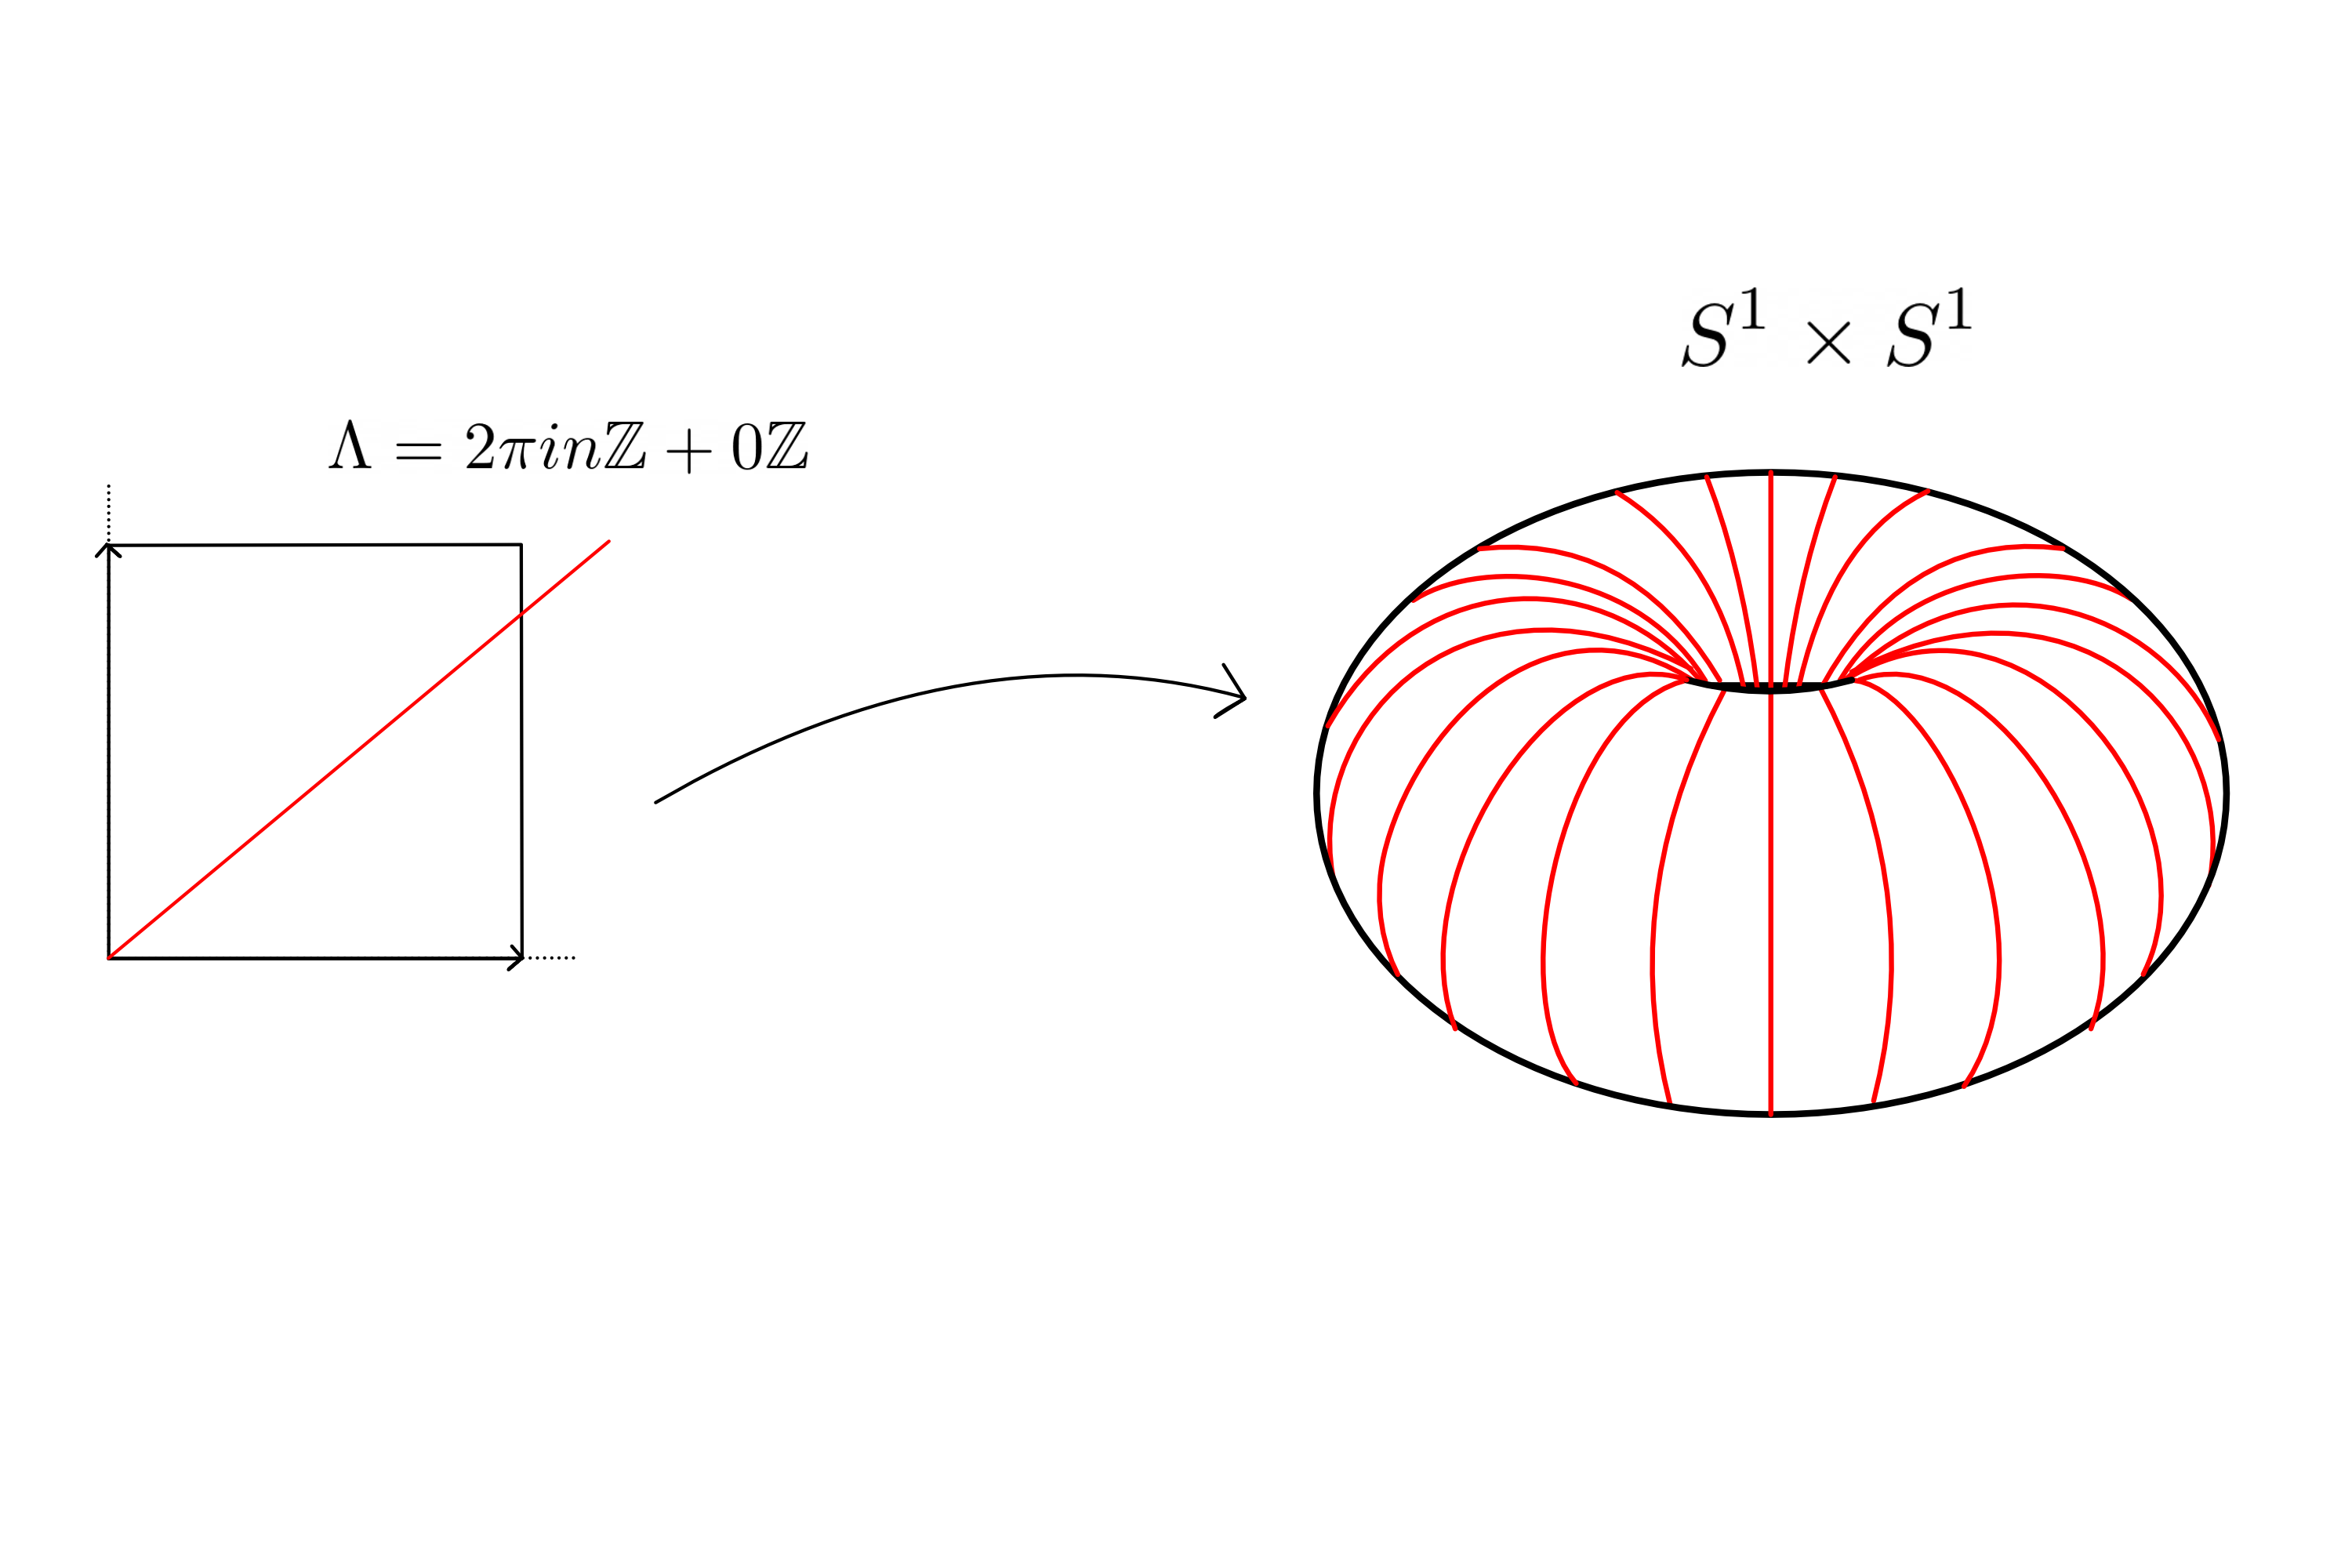
\includegraphics[width=0.7\linewidth]{Imagenes/biholomorfismo}
			\caption{Interpretación geométrica de la sucesión $z_n$.}
			\label{fig:biholomorfismo}
		\end{figure}
		
	\end{example}
	
    Como mencionabamos, el teorema de Whitney es un resultado general importante en la geometría diferencia real, pero no podemos tener un análogo directo en geometría compleja.
    
    \begin{example}\label{encajeccn}
        \textbf{No existen} subvariedades complejas compactas de $\cc^n$ de dimensión no cero. Ya que si $M\subset\cc^n$ es una subvariedad compleja compacta, entonces cada funcion de $\cc^n$ coordenada (proyección) $z_j$\footnote{Como $M$ es subvariedad, la inclusión $i:M\to \cc^n$ es holomorfa. Si $\pi_j:\cc^n\to\cc$ es la proyección a la $j$-ésima entrada, la función de $\cc^n$ coordenada $z_j=\pi_j\circ i:M\to \cc$ es una función holomorfa por ser composición de aplicaciones holomorfas.} restringida a $M$ es una función holomorfa global de $M$. Por el teorema \ref{holomorfasglobal}, $z_j$ es constante en cada componente conexa de $M$. Por lo que la inclusión $i:M\to\cc^n$ es constante en cada componente conexa de $M$. Con lo cual, cada componente conexa de $M$ consta de un único punto. Como $M$ es compacto, sólo puede tener un número finito de componentes conexas. En consecuencia, $M$ es un conjunto finito y, por tanto, tiene dimensión 0.
    \end{example}
    
    Ahora vamos a probar un resultado que nos ayudará a comprobar que una aplicación sea un encaje holomorfo. 
    
    \begin{propo}\label{encajesubvariedades}
    	Una aplicación holomorfa $f:M\to N$ es un encaje holomorfo si, y solo si, $f:M\to f(M)$ es un biholomorfismo y $f(M)\subset N$ es una subvariedad compleja.
    \end{propo}
    \begin{proof}
    		Primero, supongamos que $f:M\to N$ es un encaje. Por la condición de encaje topológico, $f:M\to f(M)$ es un homeomorfismo. En particular, la inversa $f^{-1}:f(M)\to M$ es continua.
    		
    		Tomemos $p\in M$ y sea $q=f(p)\in N$. Por la condición $(3)$ de encaje, existen cartas holomorfas $(V,\psi)$ alrededor de $q$ y $(U,\varphi)$ alrededor de $p$ tales que $f(U)\subset V$ y
    		\begin{equation*}
    			\psi\circ f\circ \varphi^{-1}(z_1,\dots,z_k)=(z_1,\dots,z_k,0,\dots,0)\in \cc^n.
    		\end{equation*}
    		Como $f$ es un homeomorfismo, $f(U)$ es abierto en $f(M)$ y $f(M)$ lleva la topología de subespacio, al reducir $V$ si es necesario podemos suponer que $V\cap f(M)=f(U)$. Entonces, en este abierto la inversa de $f$ se escribe en coordenadas como la proyección sobre las primeras $k$ coordenadas:
    		\begin{equation*}
    			\varphi\circ f^{-1}\circ \psi^{-1}(w_1,\dots,w_n)=(w_1,\dots,w_k),
    			\qquad (w_1,\dots,w_n)\in \psi(V\cap f(M)).
    		\end{equation*}
    		Esta expresión es holomorfa. Como $p$ era arbitrario, $f^{-1}$ es holomorfa en todo $f(M)$. Por tanto, $f:M\to f(M)$ es un biholomorfismo.
    		
    		Para ver que $f(M)$ es una subvariedad compleja de $N$, observemos que las mismas cartas satisfacen
    		\begin{equation*}
    			\psi(V\cap f(M))=\psi(V)\cap (\cc^k\times \{0\}).
    		\end{equation*}
  			Es decir, $f(M)$ es una subvariedad compleja de $N$.
  			
  			Ahora, supongamos que $f:M\to f(M)$ es un biholomorfismo y $f(M)$ es subvariedad compleja. Entonces es inmediato que $f:M\to f(M)$ es un encaje topológico donde $f(M)$ lleva la topología del subespacio. 
  			
  			Sea $p\in M$ y $q=f(p)\in N$. Como $f(M)$ es una subvariedad compleja, existe una carta holomorfa $(V,\psi)$ de $q$ tal que
  			\begin{equation*}
  				\psi(V\cap f(M))=\psi(V)\cap (\cc^k\times \{0\}).
  			\end{equation*} 
  			Sea $U:=f^{-1}(V)\subset M$. Entonces $f|_U:U\to V\cap f(M)$ sigue siendo un biholomorfismo. Consideremos la proyección a las primeras $k$ entradas
  			\begin{align*}
  				&\pi:\cc^n\longrightarrow \cc^k\\
  				(z_1,\dots,z_k&,\dots,z_n)\mapsto (z_1,\dots, z_k).
  			\end{align*} 
  			Definamos entonces 
  			\begin{equation*}
  				\varphi:=\pi\circ \psi\circ f|_U:U\longrightarrow\cc^k.
  			\end{equation*}
    		Como $\psi(f(V))\subset \cc^k\times \{0\}$, la aplicación restringida a $\pi$ sigue siendo un biholomorfismo sobre $\cc^k$. Por lo que, $\varphi$ es una carta holomorfa alrededor de $p$.
    		
    		Además, para todo $z\in\varphi(U)\subset\cc^k$, 
    		\begin{equation*}
    			\psi\circ f\circ \varphi^{-1}(z)=(z,0)\in\cc^n.
    		\end{equation*}
    		Por lo tanto, $f$ satisface la propiedad $(3)$ y concluimos que $f$ es un encaje holomorfo. 
    \end{proof}
    
    Un biholomorfismo sobre su imagen solo exige que existe una inversa holomorfa entre conjuntos, pero no garantiza que el dominio tenga la estructura analítica de la subvariedad imagen. En otras palabras, un encaje holomorfo es un biholomorfismo sobre su imagen cuya imagen es una subvariedad compleja. 
    
%    \begin{example}
%        Consideremos la aplicación holomorfa $f:\cc\to\pp^1$ dada por 
%        \begin{equation*}
%        	f(z)=[z:1]
%        \end{equation*}
%      	Notemos que $f$ es un homeomorfismo pues es la inversa de una carta afín de $\pp^1$. Así, determina un biholomorfismo entre $\cc$ y $\pp^1\setminus \{[1:0]\}$. Sin embargo, $\pp^1\setminus\{[1:0]\}$ no es una subvariedad compleja de $\pp^1$. Por lo tanto, $f$ no es un encaje holomorfo.
%      	\begin{figure}[H]
%      		\centering
%      		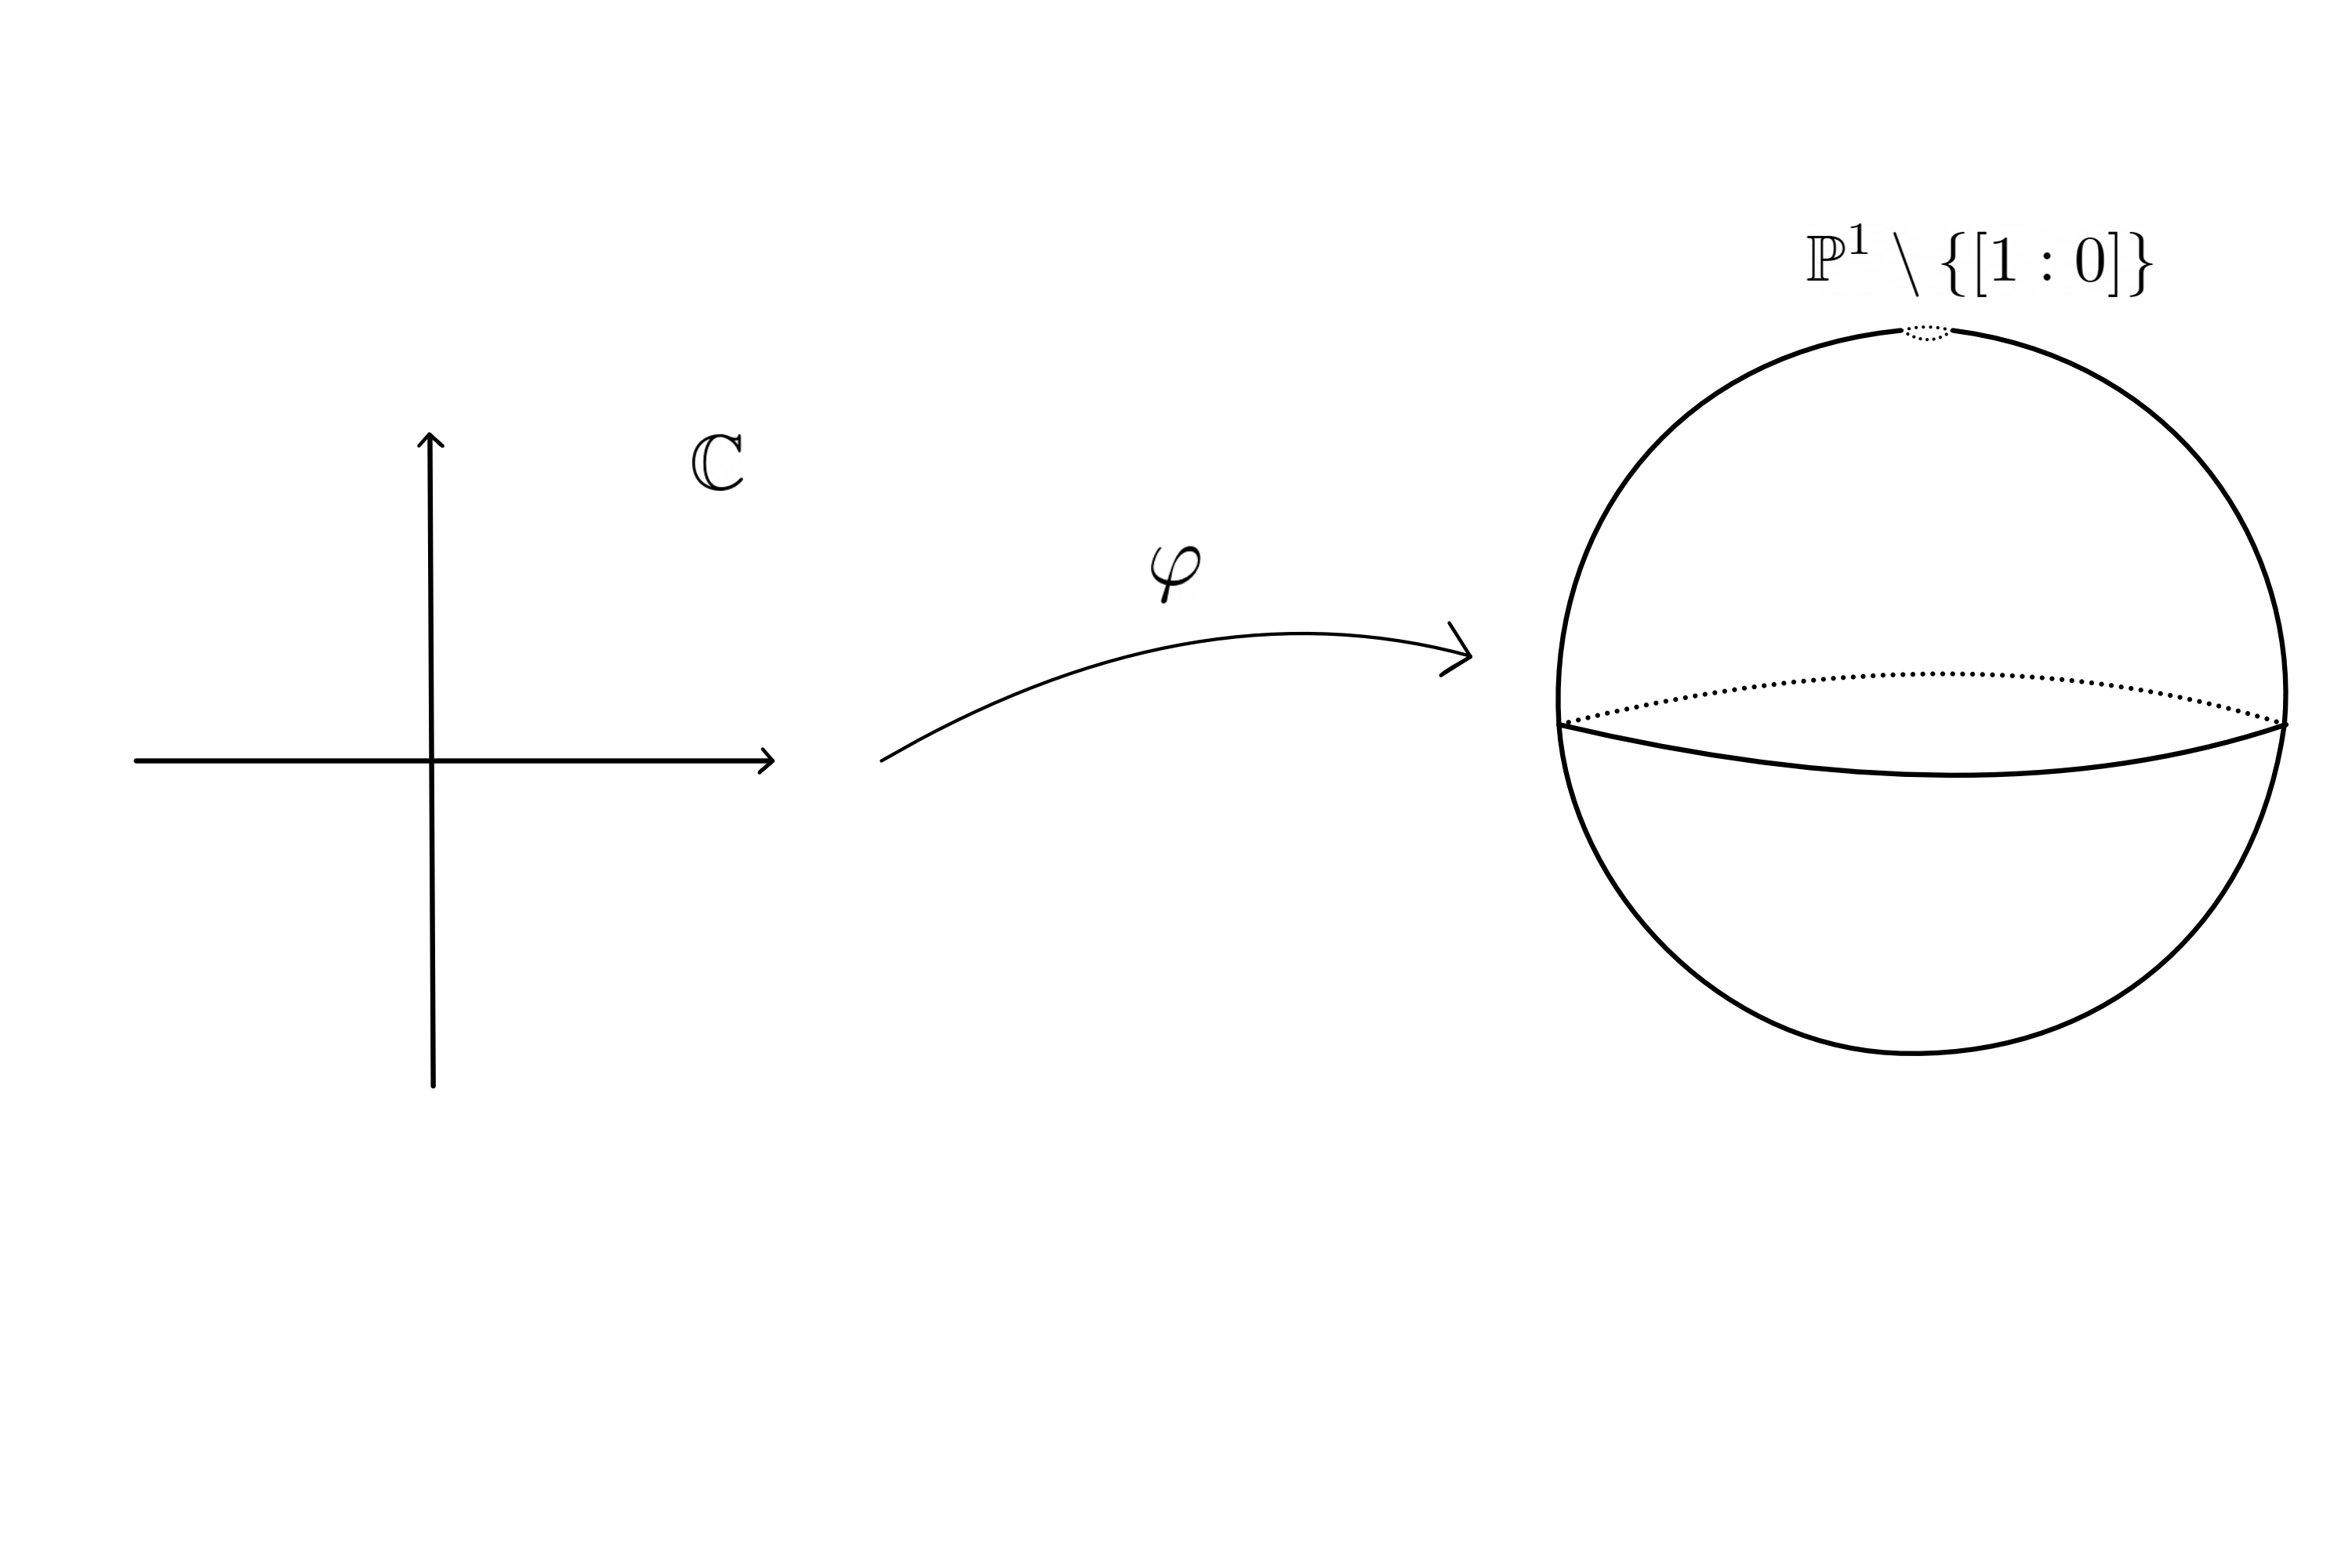
\includegraphics[width=0.5\linewidth]{Imagenes/no encaje a P1}
%      		\caption{Inmersión de $\cc$ en $\pp^1$.}
%      		\label{fig:no-encaje-a-p1}
%      	\end{figure}
%      	
%    \end{example}
   	
   	Un encaje puede entenderse, en este contexto, como una manera de \enquote{incrustar} una variedad en otra sin perder su estructura compleja. En particular, nos interesan los encajes en espacios proyectivos, cuya importancia será gracias al teorema de Chow, que abordaremos en el siguiente capítulo. Finalmente, introduzcamos la noción de una variedad que admita un encaje al espacio proyectivo.
   	
   	\begin{definition}
   		Una variedad compleja $M$ se dice \textbf{proyectiva} si admite un biholomorfismo sobre una subvariedad compleja de algún espacio proyectivo complejo.
   	\end{definition}
   	
   	\subsection{El caso de las curvas complejas}
   	
   	El problema del encaje proyectivo ya está completamente resuelto en dimensión uno. La construcción de dicho encaje constituye el antecedente directo a todo nuestro desarrollo y se basa en la teoría de divisores y el teorema de \textit{Riemann-Roch}.
   	
   	Consideremos una superficie de Riemann compacta $S$ de género $g$. Recordemos que un \textbf{divisor} sobre $S$ es una función $D:S\to \zz$ con soporte finito. Se suele escribir como una suma formal
   	\begin{equation*}
   		D=\sum_{p\in S} n_p\cdot p
   	\end{equation*}
   	donde $D(p)=n_p$ y este número es llamado \textbf{peso} de $p$.
   	
   	Por esta manera, podemos definir el \textbf{grado} del divisor $D$ como el valor finito.
   	\begin{equation*}
   		\deg(D)=\sum_{p\in S} n_p
   	\end{equation*}
   	Dado un divisor $D$, podemos considerar el \textbf{espacio de funciones meromorfas asociado al divisor} dado por el conjunto
   	\begin{equation*}
   		L(D):=\{f\in\mathscr{M}(S):\mathrm{ord}_{p}f\geq -n_p\text{ para todo }p\in S\}.
   	\end{equation*}
   	Este espacio es un $\cc$-espacio vectorial finito y su dimensión se denota como $\ell(D):=\dim_{\cc}L(D)$.\\
   	Vamos a construir una aplicación holomorfa con esta información. Consideremos $\{s_1,\cdots, s_{\ell(D)}\}$ una base del espacio $L(D)$. Sea $p\in S$, $(U,z)$ una carta alrededor de $p$ tal que $z(p)=0$ y
   	\begin{equation*}
   		k=\min_j\{\mathrm{ord}_ps_j\}.
   	\end{equation*}
   	Así, podemos escribir a $s_j$ como
   	\begin{equation*}
   		s_j=z^kg_j,
   	\end{equation*}
   	donde $g_j\in\oo_S(U)$. De esta manera, al menos una de las funciones $g_j$ no se anula en $p$, por lo que el vector
   	\begin{equation*}
   		(g_1(p),\dots,g_{\ell(D)}(p))
   	\end{equation*}
   	es no nulo y determina un punto en $\pp^{\ell(D)-1}$. Además, la definición es independiente de la carta. Con lo cual, la aplicación
   	\begin{align*}
   		\varphi_D:S\longrightarrow \pp^{\ell(D)-1}\\
   		p\mapsto[g_1(p):\cdots:g_{\ell(D)}(p)].
   	\end{align*}
   	está bien definida.
   	
   	\begin{theorem}\label{encajedesuperficies}
   		Sea $S$ una superficie de Riemann compacta de género $g$. Consideremos $D$ un divisor sobre $S$ tal que $\deg(D)\geq 2g+1$, entonces la aplicación
   		\begin{equation*}
   			\varphi_D:S\longrightarrow \pp^{\ell(D)-1}
   		\end{equation*}
   		es un encaje holomorfo.
   	\end{theorem}
   	Una demostración puede consultarse en \parencite[Teo.~5.111]{zaldrimann}. En consecuencia, toda superficie de Riemann compacta es proyectiva.
	
	Nuestro objetivo será extender esta construcción a variedades complejas de dimensión arbitraria mediante haces lineales y estudiar bajo qué hipótesis es posible obtener un encaje proyectivo.
	
\section{Haces Lineales holomorfos}

%	Un \textit{haz lineal} puede entenderse como una familia de rectas complejas parametrizadas por una variedad compleja. A cada punto $p\in M$ se le asocia un espacio vectorial complejo de dimensión uno, llamado fibra, de manera que todas estas fibras se \enquote{ensamblan} holomórficamente formando una nueva variedad $L$, denominada espacio total. Localmente, este espacio se comporta como un producto $U\times$, aunque globalmente puede presentar una geometría mucho más rica.
	
    Un \textit{haz lineal} es un objeto geométrico que asocia, a cada punto de una variedad $M$, un espacio vectorial de dimensión uno, de modo que todos estos espacios se \enquote{ensamblan} suavemente formando un nuevo espacio. Este espacio total se proyecta sobre $M$ y, cerca de cualquier punto, se ve exactamente como un producto entre un abierto y $\cc$. Así, el haz lineal puede imaginarse como una variedad \enquote{engrosada} por fibras lineales que se extienden continuamente por encima de $M$ en cada punto.

    \begin{definition}
	Sea $M$ una variedad compleja. Un \textbf{haz lineal} (holomorfo) es una triada $ (L,\pi, M) $ con la siguiente información:
	\begin{itemize}
		\item $L$ es una variedad compleja y $\pi:L\to M$ es una aplicación holomorfa sobreyectiva.
		\item Para cada punto $ p\in M $, la fibra $L_p:=\pi^{-1}(p)$ es homeomorfa a un $\cc$-espacio vectorial de dimensión $1$. Esto es, $L_p\cong \cc$. 
		\item Existe una cubierta de $\{U_i\}_{i\in I}$ de $M$ y biholomorfismos 
		\begin{align*}
			\phi_i:\pi^{-1}(U_i)\to U_i\times\cc,
		\end{align*}
		llamados \textbf{trivialización local}, tales que el siguiente diagrama conmuta
		\begin{center}
			\begin{tikzcd}
				{L|_{U_i}:=\pi^{-1}(U_i)} && {U_i\times\cc} \\
				\\
				& M
				\arrow["{\phi_i}", from=1-1, to=1-3]
				\arrow["\pi"', from=1-1, to=3-2]
				\arrow["{pr_1}", from=1-3, to=3-2]
			\end{tikzcd}
		\end{center}
		y si $ p\in U_i$, entonces la restricción a las fibras es un morfismo de $ \cc $-espacios vectoriales
		\begin{center}
			\begin{tikzcd}
				{L_p=\pi^{-1}(p)} && {\{p\}\times \cc\subset U_i\times\cc} && {\cc}
				\arrow["\phi_i|_{L_p}", from=1-1, to=1-3]
				\arrow["{\pi_2}", from=1-3, to=1-5]
			\end{tikzcd}
		\end{center}
		
		\begin{figure}[H]
			\centering
			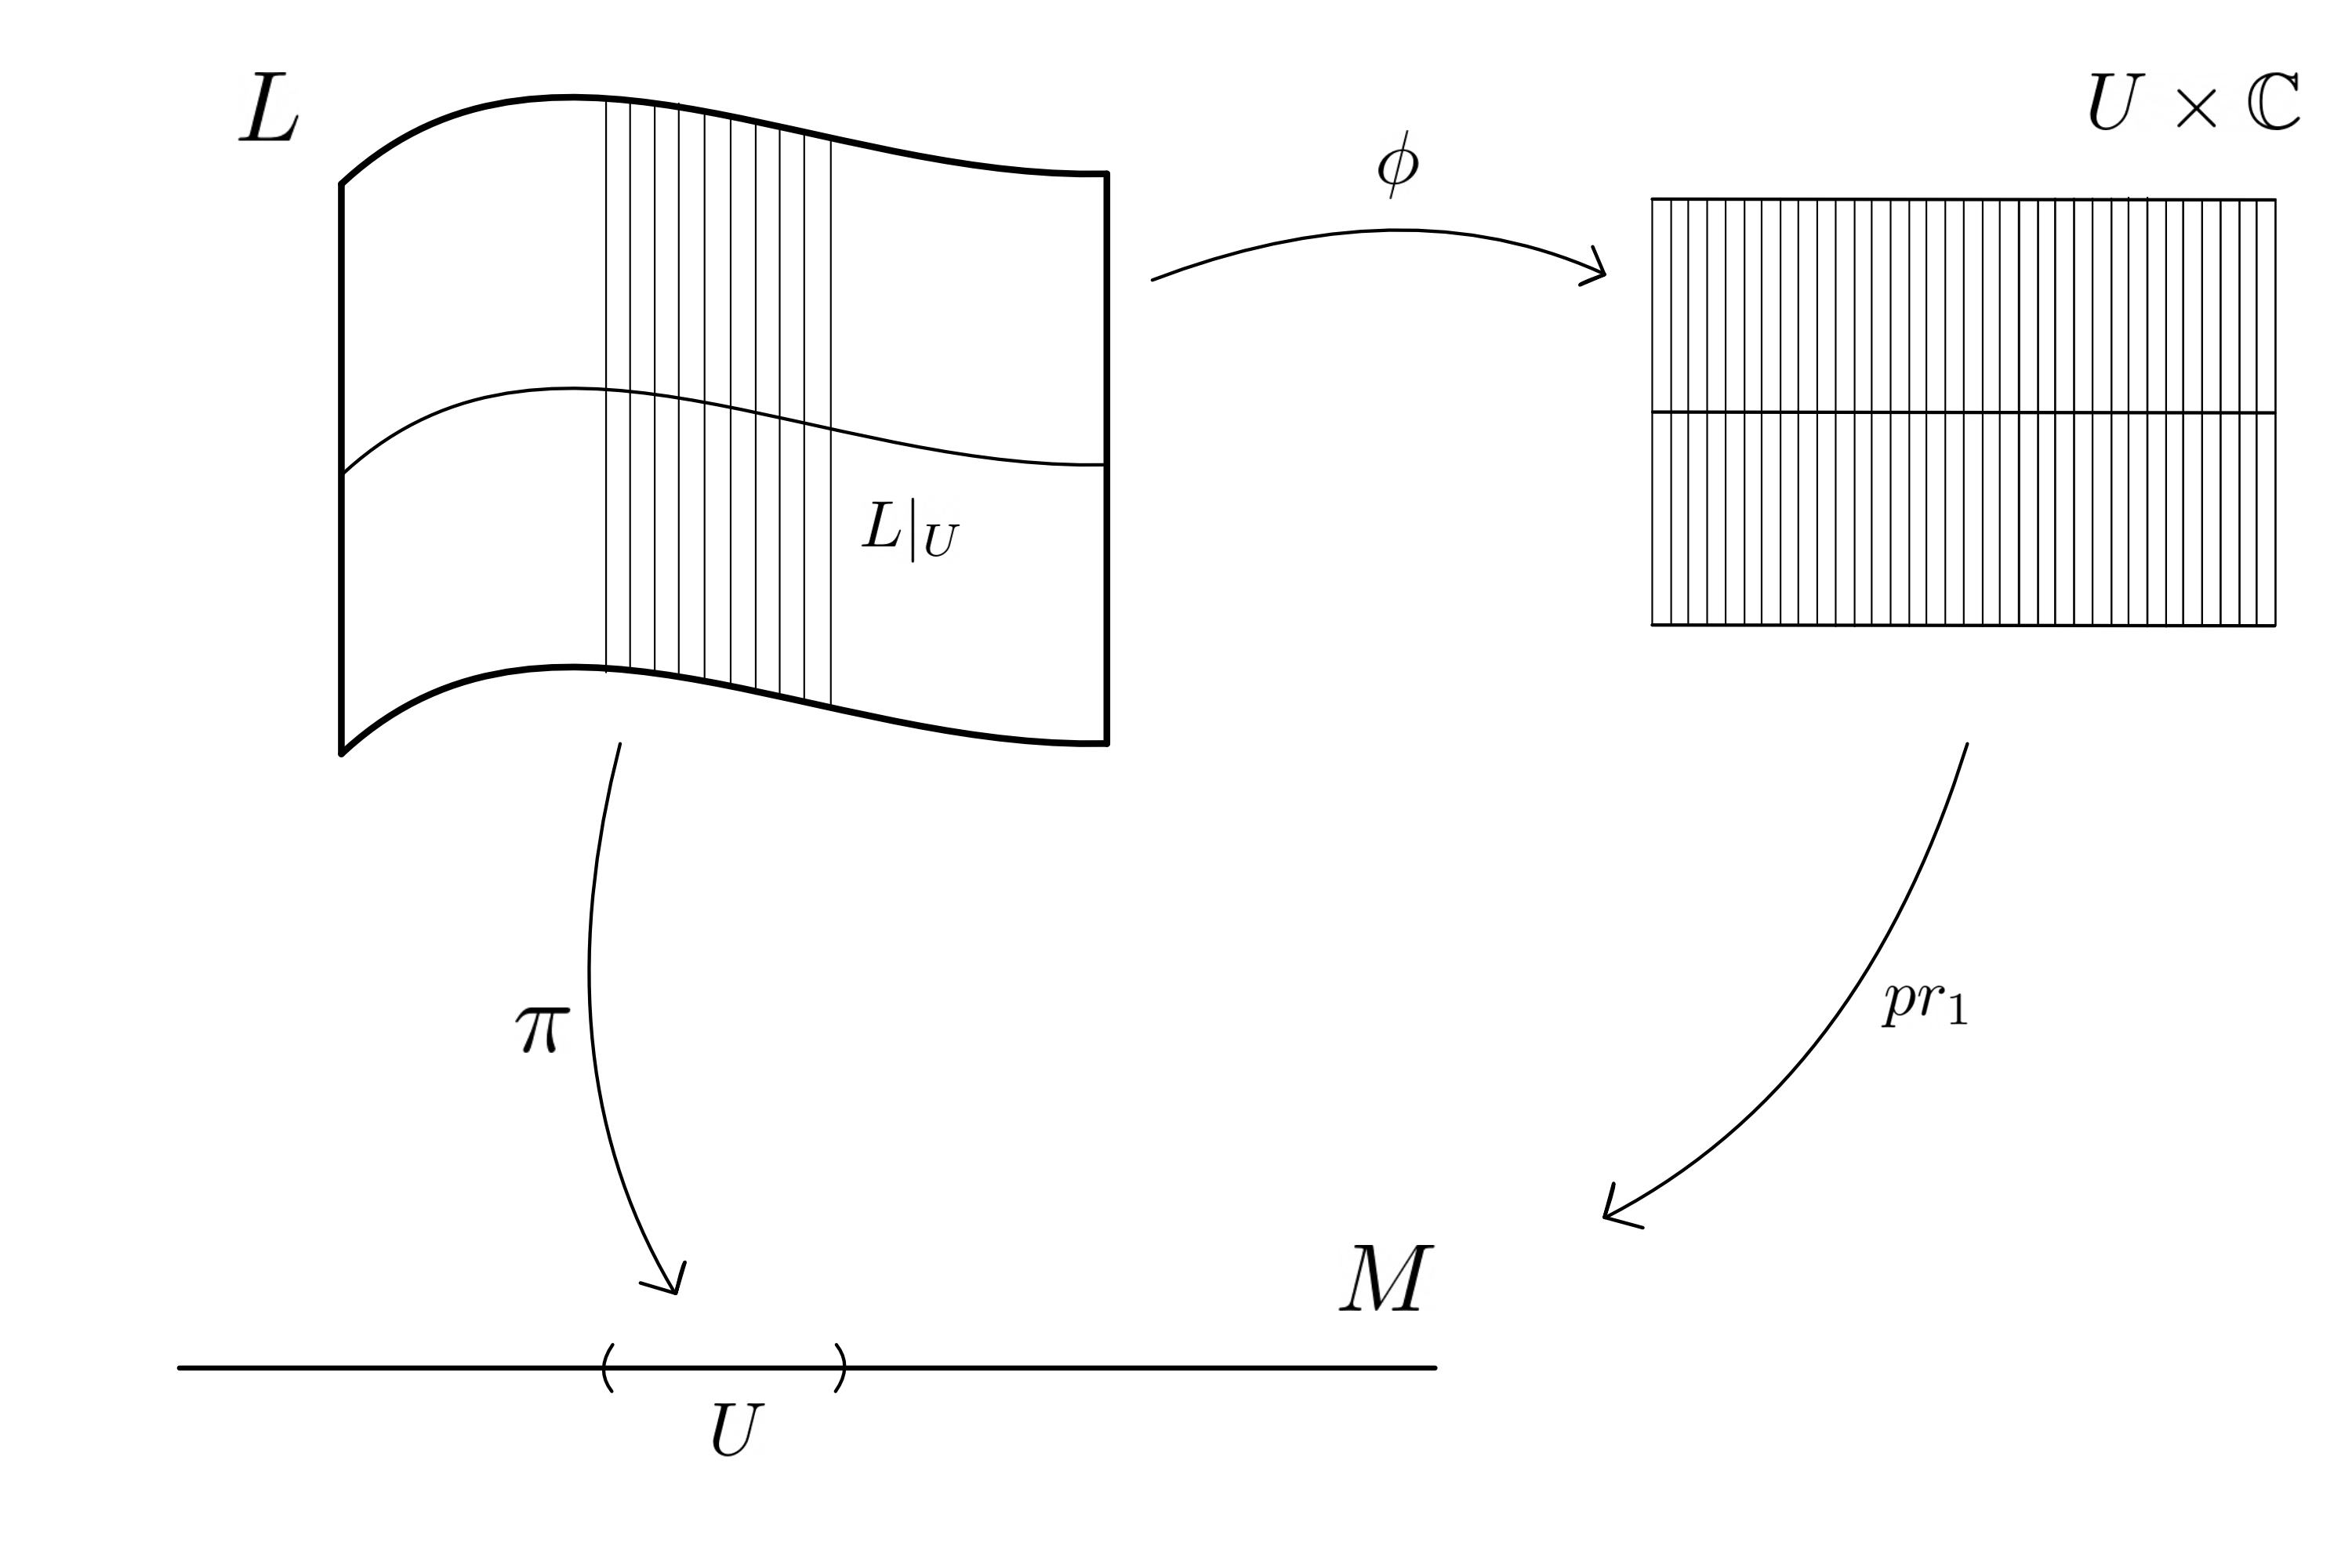
\includegraphics[width=0.7\linewidth]{Imagenes/definicion de haz}
			\caption{Una trivialización de un haz lineal.}
			\label{fig:definicion-de-haz}
		\end{figure}
		
	\end{itemize}
    \end{definition}

    \begin{remark}
    	Sea $ (L,\pi, M) $ es un haz lineal holomorfo. Al espacio $M$ se le llama \textbf{espacio base}, al espacio $ L $ se le llama \textbf{espacio total} y a la función sobreyectiva $\pi:L\to M$ se le llama \textbf{proyección}. Cuando la proyección es clara, se suele denotar $ L\longrightarrow M$ o
    	\begin{center}
    		\begin{tikzcd}
    			L \\
    			\\
    			M
    			\arrow[no head, from=1-1, to=3-1]
    		\end{tikzcd}
    	\end{center}
    	Y si el espacio base también es claro o es fijo, solo decimos que $L$ es un haz lineal. 
    \end{remark}

    \begin{example}[Haz trivial]\label{haztrivial}
    	Sea $M$ un espacio topológico. Notemos que el espacio producto $L:=M\times\cc$ tiene una función proyección a la primera entrada
    	\begin{align*}
    		\pi:&M\times\cc\longrightarrow M\\
    		&(p,z)\mapsto p
    	\end{align*}
    	la cual es holomorfa y sobreyectiva. Si $p\in M$, entonces
    	\begin{align*}
    		L_p=\pi^{-1}(p)=\{p\}\times\cc\cong \cc.
    	\end{align*}
    	Luego, para toda cubierta $\{U_i\}_{i\in I}$ de $M$, tenemos que 
    	\begin{align*}
    		L|_{U_i}=\pi^{-1}(U_i)=U_i\times \cc.
    	\end{align*} 
    	Así, la trivialización local está dada por $\{U_i\}_{i\in I}$ y los biholomorfismos identidad $id_i:L|_{U_i}\to U_i\times\cc$ y claramente conmuta el diagrama
    	\begin{center}
    		\begin{tikzcd}
    			{L|_{U_i}:=\pi^{-1}(U_i)} && {U_i\times\cc} \\
    			\\
    			& M
    			\arrow["{id_i}", from=1-1, to=1-3]
    			\arrow["\pi"', from=1-1, to=3-2]
    			\arrow["{\pi_1}", from=1-3, to=3-2]
    		\end{tikzcd}
    	\end{center}
    	Por lo tanto, $(M\times\cc,\pi_1,M)$ es un haz lineal sobre $M$. 
    \end{example}
    
    Sea $L$ un haz lineal sobre la variedad compleja $M$. Tomemos una trivialización ${U_i}*{i\in I}$ de $L$. Es decir, para cada $i$ existe un biholomorfismo
    \begin{equation*}
    	\psi_i :L|_{U_i}\longrightarrow U_i\times \mathbb{C}
    \end{equation*}
    En una intersección $U_{ij}:=U_i\cap U_j$, ambas trivializaciones difieren por multiplicación por una función holomorfa no nula
    \begin{equation*}
    	\psi_i\circ \psi_j^{-1}(x,z)=(x,g_{ij}(x)z),
    	\qquad x\in U_i\cap U_j,
    \end{equation*}
    donde
    \begin{equation*}
    	g_{ij}\in \mathcal{O}^*(U_i\cap U_j).
    \end{equation*}
    
    \begin{figure}[H]
    	\centering
    	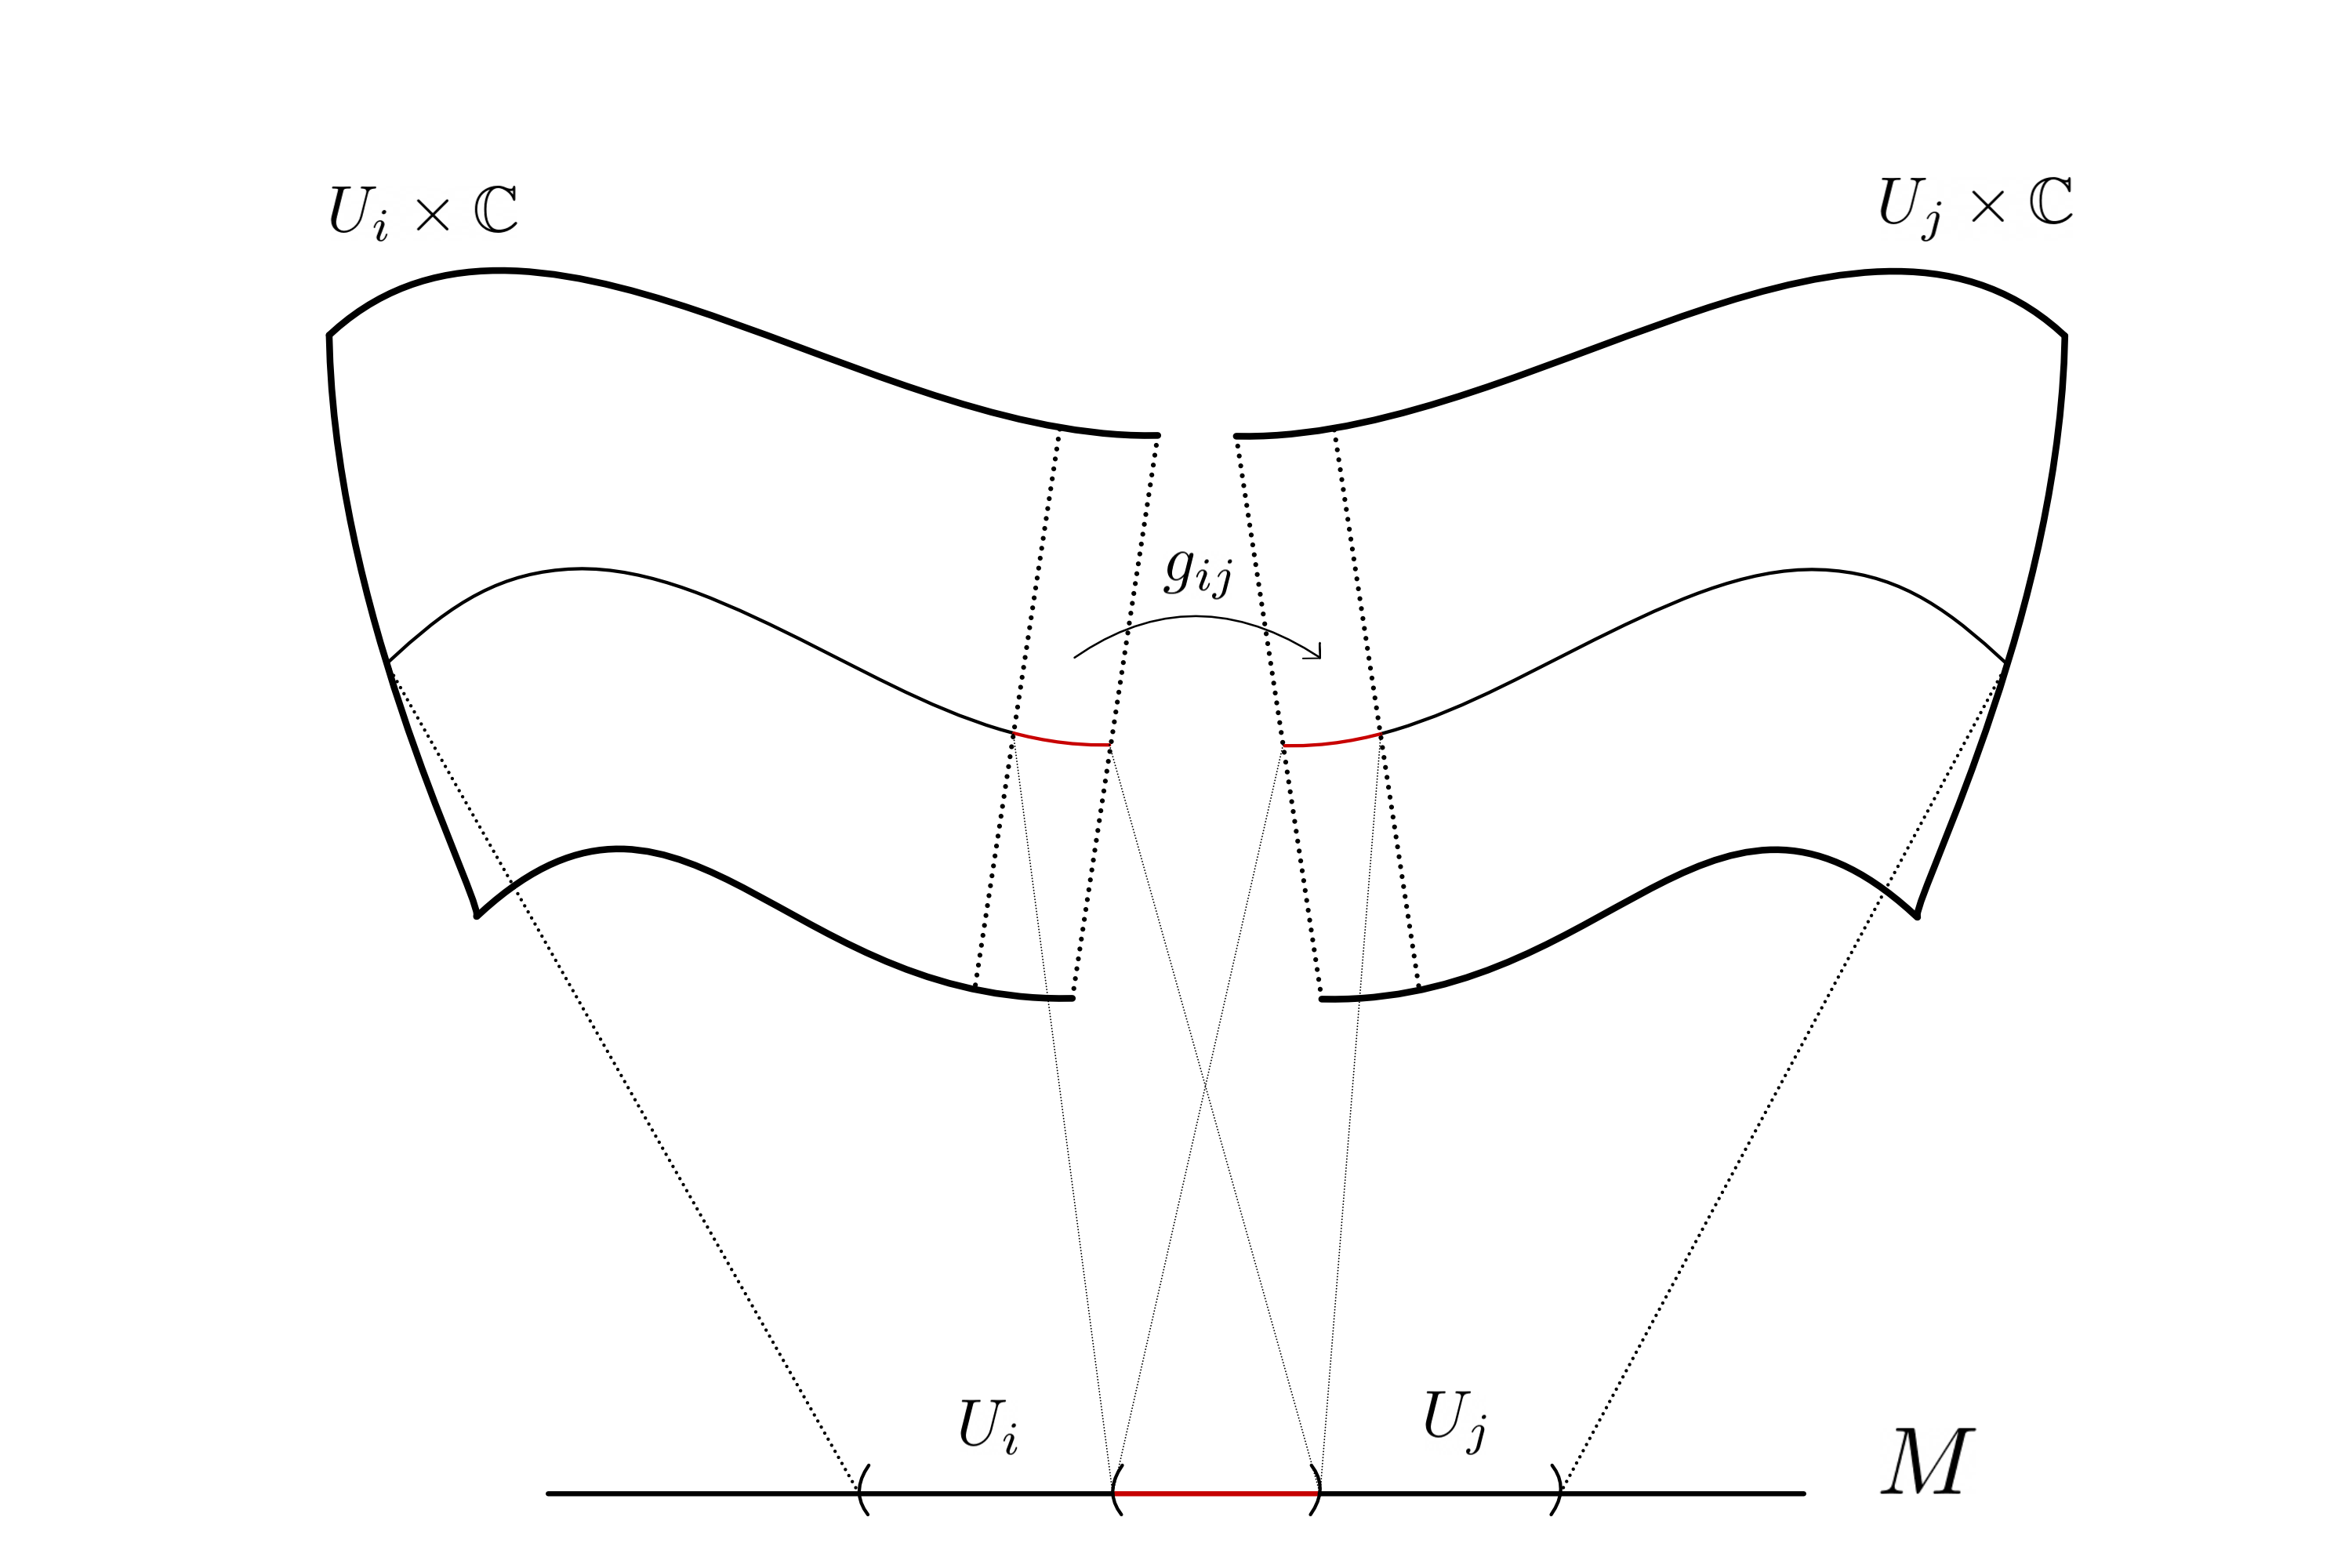
\includegraphics[width=0.5\linewidth]{Imagenes/funciones de transición}
    	\caption{Representación de las funciones de transición}
    	\label{fig:funciones-de-transicion}
    \end{figure}
    
    \begin{remark}\label{cociclos}
    	A las funciones $g_{ij}$ se le llaman \textbf{funciones de transición} y cumplen dos propiedades
    	\begin{align*}
    		g_{ii}&=1,\qquad \text{en }\enspace U_i;\\
    		g_{ij}g_{jk}g_{ki}&=1,\qquad \text{en }\enspace U_i\cap U_j\cap U_k.
    	\end{align*}
    	llamadas \textbf{condiciones de cociclo}.
    \end{remark}

	\begin{example}\label{gijhaztrivial}
		Consideremos el haz trivial $L=M\times \cc$. Por el ejemplo \ref{haztrivial}, sabemos que para cualquier cubierta $\{U_i\}_{i\in I}$ de $M$ se tiene la trivialización
		\begin{align*}
			\psi_i=L|_{U_i}\longrightarrow U_i\times \cc\\
			(p,z)\mapsto (p,z).
		\end{align*}
		Por lo tanto, las funciones de transición de $L$ están dadas por
		\begin{equation*}
			g_{ij}=1,\qquad \text{para todo }i,j\in I.
		\end{equation*}
	\end{example}
	
	Las funciones de transición contienen toda la información necesaria para reconstruir el haz lineal. De hecho, dos haces son isomorfos si y solo si sus funciones de transición representan el mismo cociclo, y recíprocamente, toda colección de funciones que satisfaga las condiciones de cociclo determina un haz lineal.
    
    \begin{propo}[Construcción de un haz holomorfo]
	   Sea $M$ una variedad compleja y $\{U_i\}_{i\in I}$ una cubierta de $M$. Supongamos que para cada $i$ y $j$ tal que $ U_{ij} \neq \emptyset$ tenemos una función holomorfa $g_{ij}:U_{ij}\to \cc^*$ tales que satisfacen las condiciones de cociclos, entonces existe un haz lineal holomorfo $ L\longrightarrow M $ que admite una trivialización en $\{U_i\}_{i\in I}$ y con funciones de transición $g_{ij}$.
    \end{propo}
	\begin{proof}
		\parencite[Chap. 3, Sec. 1, Prop. 3.5]{leecomplex}.
	\end{proof}

\subsection{Operaciones con haces lineales}

	De la proposición anterior se sigue que, para construir un haz lineal, basta definir funciones de transición que satisfagan la condición de cociclo. Esta observación proporciona un método natural para obtener nuevos haces lineales a partir de otros ya dados mediante sus funciones de transición.

\begin{definition}
	Sean $L$ y $L'$ dos haces lineales sobre $M$, con funciones de transición $\{U_i,g_{ij}\}$ y $\{U'_i,g'_{ij}\}$, respectivamente.
	\begin{enumerate}
		\item Definimos el \textbf{haz dual} de $L$, denotado por $L^*$, como el haz lineal cuyas funciones de transición son
		\begin{equation*}
			g_{ij}^{-1}:=\frac{1}{g_{ij}}.
		\end{equation*}
		\item Definimos el \textbf{producto tensorial} $L\otimes L'$ como el haz lineal cuyas funciones de transición son
		\begin{equation*}
			g_{ij}g'_{ij},
		\end{equation*}
		en las intersecciones donde ambas estén definidas\footnote{Las funciones de transición no tienen por qué estar definidas sobre los mismos abiertos. En tal caso, se considera un refinamiento común de las cubiertas, obtenido al intersectar los abiertos de ambas cubiertas.}.
		
		\item Para $k\in \mathbb{N}$, se denota
		\begin{equation*}
			L^{k}:=\underbrace{L\otimes\cdots\otimes L}_{k\text{ veces}},
		\end{equation*}
		al $k$-ésimo producto tensorial de $L$ consigo mismo. Además, usamos la notación 
		\begin{equation*}
			L^{-k}:=(L^*)^k
		\end{equation*}
	\end{enumerate}
\end{definition}	

	
	
	\begin{example}\label{Ltensordual}
		Sea $L$ un haz lineal sobre $M$ con funciones de transición $\{U_i,g_{ij}\}$ de $M$, entonces las funciones de transición de $L\otimes L^*$ están dadas por
		\begin{equation*}
			g_{ij}g_{ij}^{-1}=1,\qquad\text{para todo }i,j\in I.
		\end{equation*}
		Por el ejemplo \ref{gijhaztrivial}, el haz lineal $L\otimes L^*$ corresponde con el haz trivial de $M$.
	\end{example}
	
	\begin{definition}
		Sea $f:N\to M$ una aplicación holomorfa y $\pi:L\to M$ un haz lineal sobre $M$. El \textbf{pullback} de $L$ a través de $f$ es el espacio 
		\begin{equation*}
			f^*L=\{(n,l)\in N\times L: f(n)=\pi(l)\}.
		\end{equation*}
		junto a las aplicaciones naturales
		\begin{align*}
			\pi':f^*L\longrightarrow N\\
			(n,l)\mapsto n
		\end{align*}
		\begin{align*}
			h:f^*L\longrightarrow L\\
			(n,l)\mapsto l
		\end{align*}
		de forma que el siguiente diagrama conmuta
		\begin{center}
			\begin{tikzcd}
				{f ^*L} && L \\
				\\
				N && M
				\arrow["{h}", from=1-1, to=1-3]
				\arrow["{\pi'}"', from=1-1, to=3-1]
				\arrow["\pi", from=1-3, to=3-3]
				\arrow["f"', from=3-1, to=3-3]
			\end{tikzcd}
		\end{center}
	\end{definition}
	
	\begin{remark}
		Si $\{U_i\}_{i\in I}$ es una cubierta de $M$ sobre la cual $L$ se trivializa, con funciones de transición
		\begin{equation*}
				g_{ij}\in \mathcal{O}^*(U_i\cap U_j),
		\end{equation*}
		entonces el pullback $f^*L\to N$ se trivializa sobre la cubierta inducida $\{f^{-1}(U_i)\}_{i\in I}$ de $N$.
		
		En efecto, sobre cada $f^{-1}(U_i)$ definimos la trivialización local de $ f^*L$ usando la trivialización de $L$ sobre $U_i$. Si
		\begin{equation}
			\psi_i:\pi^{-1}(U_i)\longrightarrow U_i\times \mathbb{C}
		\end{equation}
		es una trivialización de $L$, entonces se obtiene una trivialización de $f^*L $ sobre $f^{-1}(U_i) $ dada por
		\begin{align*}
			\widetilde{\psi}_i:f^*L|_{f^{-1}(U_i)}&\longrightarrow f^{-1}(U_i)\times \mathbb{C}\\
			(n,\ell)&\mapsto \bigl(n, z\bigr),
		\end{align*}
		donde $\psi_i(\ell)=(f(n),z)$. Ahora, en una intersección $f^{-1}(U_{ij})$, el cambio de trivialización viene dado por
		\begin{equation*}
			\widetilde{\psi}_i\circ \widetilde{\psi}_j^{-1}(n,z)=\bigl(n, (g_{ij}\circ f)(n) z\bigr).
		\end{equation*}
		Por tanto, las funciones de transición del pullback $f^*L$ son precisamente
		\begin{equation*}
			(f^*g)_{ij}=g_{ij}\circ f
			\quad\text{en}\quad
			f^{-1}(U_{ij}).
		\end{equation*}
	\end{remark}

\subsection{Espacio de secciones}

	\begin{definition}
		Sea $\pi:L\to M$ un haz lineal sobre una variedad compleja $M$. Una \textbf{sección} (global) de $L$ es una aplicación holomorfa $s:M\to L$ tal que
		\begin{equation*}
			\pi\circ s=\mathrm{id}_M.
		\end{equation*}
		Una \textbf{sección local} es una sección $s:U\to L$ definida solo en un abierto $U\subset M$. 
		\begin{figure}[H]
			\centering
			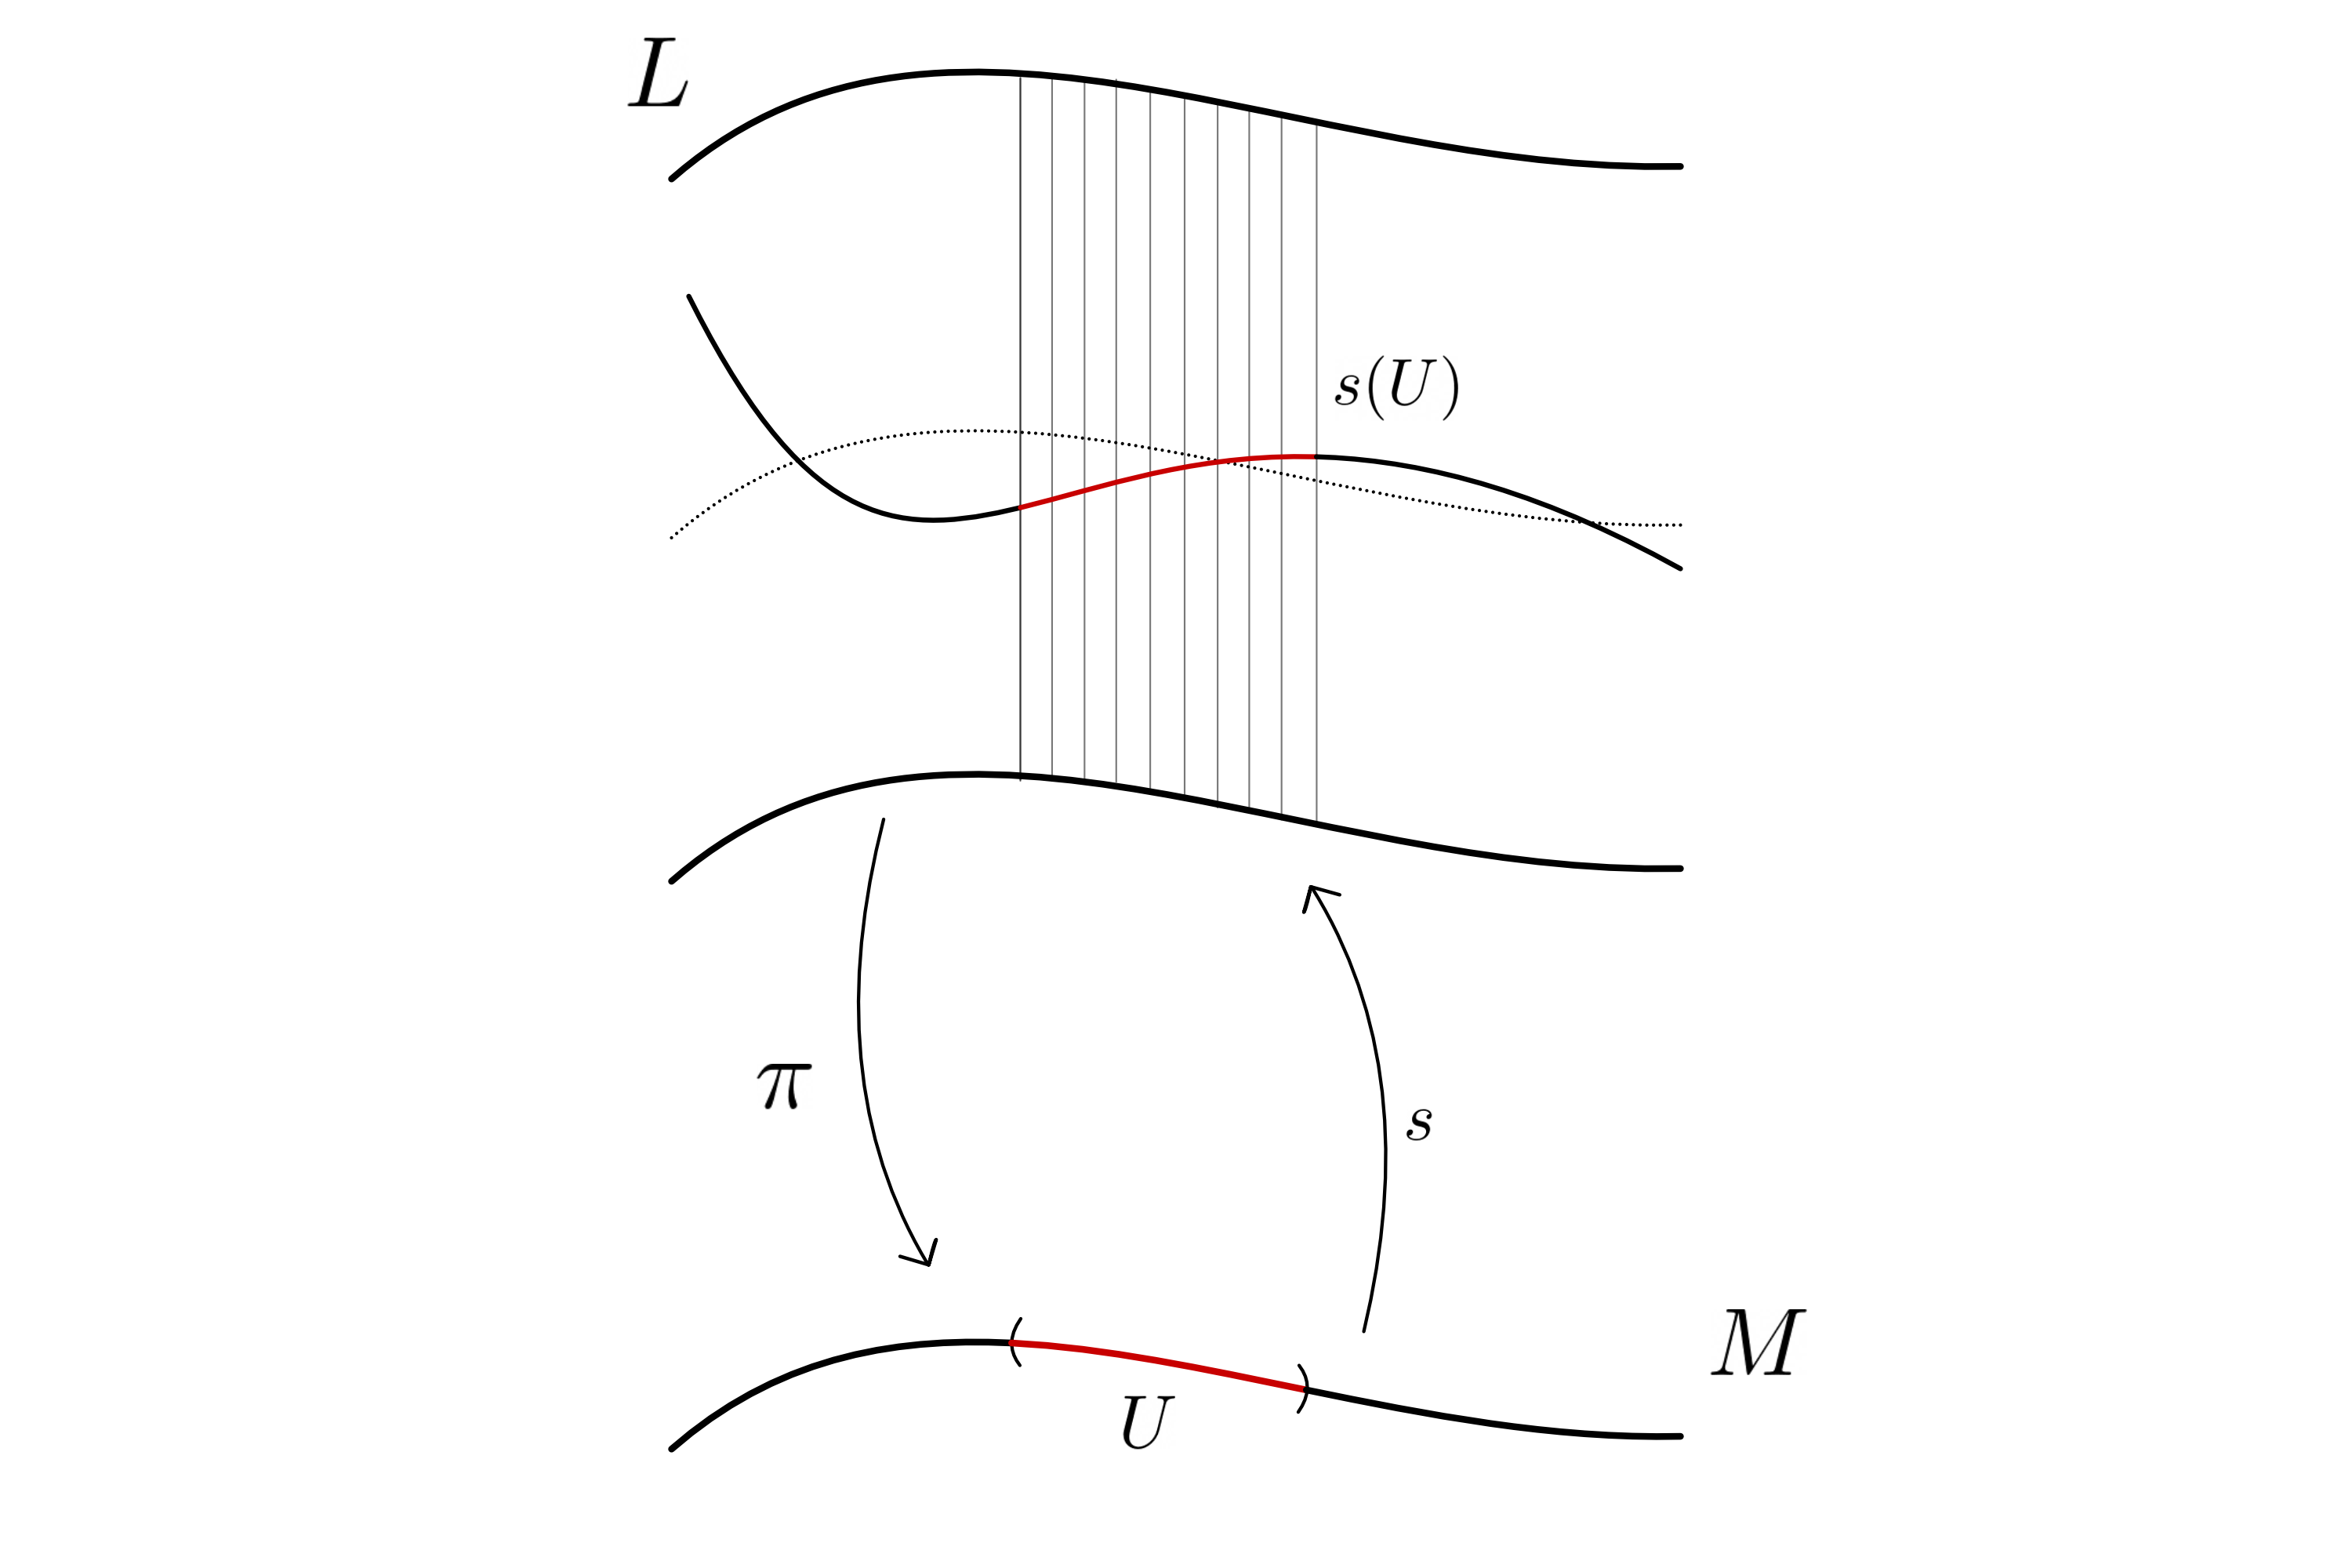
\includegraphics[width=0.5\linewidth]{Imagenes/seccion local}
			\caption{Interpretación de las secciones locales}
			\label{fig:seccion-local}
		\end{figure}
		
	\end{definition}
	
	Si $p\in M$ y $s:M\to L$ es una sección global, entonces $\pi(s(p))=p$. Así, $s(p)\in \pi^{-1}(p)=L_p$. Esto significa que las secciones $s$ siempre mandan a los puntos $p\in M$ a sus fibras $L_p$. Entonces, podemos pensar que una sección encaja a $M$ dentro de $L$ de manera que intersecta solo una vez a cada fibra. En particular, existe siempre una sección $s_0:M\to L$ definida como
	\begin{equation*}
		s_0(p)=0\in L_p,\qquad \text{para todo }p\in M.
	\end{equation*}
	La sección $s_0$ es llamada \textbf{sección cero} de $L$.
	
	\begin{definition}
		Sea $M$ una variedad compleja y $\pi:L\to M$ un haz lineal. Definimos el \textbf{espacio de secciones holomorfas} como
		\begin{equation*}
			\oo(U;L):=\{s:U\to L: s\text{ es una sección local de }L\}.
		\end{equation*}
	\end{definition}
	
	\begin{remark}\label{seccionlocalholomorfa}
		Sea $\pi:L\to M$ un haz lineal y $s:U\to L$ una sección local. Por definición
		\begin{equation}\label{pis(p)}
			\pi \circ s(p)=p,\qquad p\in U.
		\end{equation} 
		Supongamos que $L$ se trivializa en $U$, entonces
		\begin{equation*}
			\psi:\pi^{-1}(U)\cong U\times \cc.
		\end{equation*}
		Como $s(p)$ pertenece a la fibra de $p$, tenemos que
		\begin{equation*}
			s(p)\in \pi^{-1}(U)\cong U\times \cc.
		\end{equation*}
		Por (\ref{pis(p)}), tenemos que $s$ conmuta con la proyección a la primera entrada. Por lo que
		\begin{equation*}
			\psi(s(p))=(p,z)\in U\times \cc.
		\end{equation*}
		Como $s$ es holomorfa, existe una función holomorfa $f\in \oo_M(U)$ tal que
		\begin{equation*}
			\psi(s(p))=(p,f(p)).
		\end{equation*}
		Más aún, consideremos una intersección de abiertos trivializantes $U_i\cap U_j$ con funciones de transición $g_{ij}$. Entonces
		\begin{equation*}
			\psi_i(s(p))=(p,f_i(p)),\qquad \psi_j(s(p))=(p,f_j(p)).
		\end{equation*}
		Por definición de las funciones de transición
		\begin{equation*}
			\psi_i\circ \psi_j^{-1}(p,z)=(p,g_{ij}(p)z).
		\end{equation*}
		De esta manera,
		\begin{equation*}
			(p,f_i(p))=\psi_i(s(p))=\psi_i(\psi_j^{-1}(p,f_j(p)))=(p,g_{ij}(p)f_j(p)).
		\end{equation*}
		Por lo tanto, 
		\begin{equation*}
			f_i(p)=g_{ij}(p)f_j(p).
		\end{equation*}
	\end{remark}
	
	Notemos que las secciones holomorfas de un haz lineal pueden sumarse y multiplicarse por escalares complejos, gracias a la estructura de $\cc$-espacio vectorial de las fibras. Además, por la observación anterior, estas operaciones preservan la holomorfía, pues se reducen punto a punto a operaciones entre funciones holomorfas. En consecuencia, tenemos lo siguiente:
	
	\begin{propo}
		Sea $M$ una variedad compleja y $\pi:L\to M$ un haz lineal. Entonces el funtor definido por
		\begin{align*}
			\mathcal{O}(L)(U):=\mathcal{O}(U;L)
		\end{align*}
		para todo abierto $U$ de $M$, es una gavilla de $\cc$-espacios vectoriales.
	\end{propo}
	
	La demostración de esta proposición es análoga a la de la gavilla de funciones holomorfas. Además, las secciones holomorfas pueden multiplicarse por funciones holomorfas locales y el resultado sigue siendo una sección holomorfa. Esto muestra que la gavilla $\mathcal{O}(L)(\_)$ posee de manera natural una estructura de gavilla de $\mathcal{O}_M$-módulos. En particular, por la observación \ref{seccionlocalholomorfa}, dicha gavilla es localmente isomorfa a $\mathcal{O}_M$; es decir, $\mathcal{O}(L)(\_)$ es una gavilla de $\mathcal{O}_M$-módulos localmente libre de rango $1$. Por lo tanto, $\mathcal{O}(L)(\_)$ es una gavilla coherente (véase \parencite[Chap.~5, Sec.~3.4]{griffiths}).

	\begin{example}\label{seccionesdeltrivial}
		Consideremos el haz trivial $L$ sobre $M$ y tomemos $U$ un abierto no vacío de $M$. Entonces
		\begin{equation*}
			\pi^{-1}(U)= U\times \cc.
		\end{equation*}
		Por la observación \ref{seccionlocalholomorfa}, tenemos que si $s$ es una sección local sobre $U$ entonces
		\begin{equation*}
			s(p)=(p,f(p)),\qquad \text{para todo }\ p\in U,
		\end{equation*}
		donde $f\in\oo_M(U)$. De esta manera, $s$ está totalmente determinada por la función holomorfa $f$. Asimismo, toda función holomorfa $f$ de $M$ determina una sección local de $L$. Por lo tanto, la gavilla $\mathcal{O}(L)$ corresponde con la gavilla de funciones holomorfas $\oo_M$.
	\end{example}
	
	\begin{theorem}
		Sea $M$ una variedad compleja compacta y $\pi:L\to M$ un haz lineal. Entonces el espacio de secciones globales $	H^0(M,L):=\mathcal{O}(M;L)$ \footnote{La notación proviene del hecho de que el espacio de secciones globales coincide con el grupo de cohomología de Čech de grado $0$ de la gavilla asociada al haz lineal $L$.} es un $\cc$-espacio vectorial de dimensión finita.
	\end{theorem}
	
	Este resultado muestra nuevamente la rigidez de la geometría compleja, pues aunque un haz lineal pueda admitir muchas secciones locales, la compacidad de la variedad impone una fuerte restricción sobre las secciones holomorfas globales. En general, la finitud de $H^0(M,L)$ se deduce del hecho de que la gavilla $\mathcal{O}(L)(\_)$ es coherente (véase \parencite[Chap.~VIII, Sec.~A, Cor.~10]{gunningrossi}). Sin embargo, también puede obtenerse mediante argumentos analíticos más elementales, introduciendo una norma global sobre $\mathcal{O}(M;L)$ y demostrando que la bola unitaria cerrada es compacta (véase \parencite[Chap.~3, Sec.~1, Theo.~3.13]{leecomplex}).
	
	\begin{example}\label{H0deltrivial}
		Consideremos el haz trivial $L$ sobre $M$. Por el ejemplo \ref{seccionesdeltrivial} tenemos que
		\begin{equation*}
			H^0(M,L)\cong \oo_M(M).
		\end{equation*} 
		Si $M$ es compacta, toda función holomorfa global es constante (véase teorema \ref{holomorfasglobal}), luego
		\begin{equation*}
			H^0(M,L)\cong\cc.
		\end{equation*}
		Por lo tanto,
		\begin{equation*}
			\dim_\cc H^0(M,L)=1.
		\end{equation*}
	\end{example}
	
	\begin{example}[Secciones del pullback]\label{seccionespullback}
		Sea $f:N\to M$ una aplicación holomorfa y $\pi:L\to M$ un haz lineal. Recordemos que el pullback está dado por
		\begin{equation*}
			f^*L=\{(n,l)\in N\times L:f(n)=\pi(l)\}.
		\end{equation*}
		Sea $s\in H^0(M,L)$ una sección global de $L$. Definamos
		\begin{align*}
			f^*s&:N\longrightarrow f^*L\\
			f^*s(n)&=(n,s(f(n))).
		\end{align*}	
		Es inmediato que $f^*s$ es holomorfa y 
		\begin{equation*}
			(\pi'\circ f^*s)(n)=\pi'(f^*s(n))=\pi'(n,s(f(n)))=n.
		\end{equation*}
		De esta manera, $f^*s$ es una sección global de $f^*L$. Notemos además que esta construcción determina una aplicación $\cc$-lineal
		\begin{equation*}
			f^*:H^0(M,L)\longrightarrow H^0(N,f^*L).
		\end{equation*}
		En general, $f^*$ no es sobreyectiva. Por ejemplo, tomemos $M=\{\mathrm{pt}\}$ y $L=\cc$ es haz trivial sobre $M$. Entonces $H^0(M,L)\cong\cc$, mientras que para cualquier variedad compleja $N$ se tiene que
		\begin{equation*}
			H^0(N,f^*L)\cong H^0(N,N\times \cc)=\oo_N(N).
		\end{equation*} 
		Tomando $N=\cc$, entonces $\oo_N(N)$ tiene dimensión infinita pues $N$ no es compacta. Por lo que $f^*$ determina un morfismo lineal
		\begin{equation*}
			\cc\longrightarrow \oo(\cc).
		\end{equation*}
		el cual no es sobreyectivo.
	\end{example}
	
\section{Haces amplios y encajes}

Los haces lineales son importantes en el estudio de los encajes al espacio proyectivo porque actúan como el mecanismo que nos permite construir aplicaciones holomorfas desde una variedad compleja hacia $\pp^N$. Sin la estructura de los haces lineales, no existiría una forma natural de generar las coordenadas homogéneas necesarias para \enquote{sumergir} una variedad compleja en el mundo algebraico del espacio proyectivo. 

\subsection{Haces lineales del espacio proyectivo}

	Consideremos el espacio proyectivo $\pp^n$ y definamos el conjunto
	\begin{equation*}
		\mathcal{O}(-1)=\{(l,z)\in\pp^n\times \cc^{n+1}:l\in\pp^n, z\in l\text{ ó }z=0\}.
	\end{equation*}
	Notemos que la proyección a la primera entrada $\pi:\mathcal{O}(-1)\to\pp^n$ es una aplicación holomorfa sobreyectiva. Con esto podemos ver que:
	
	\begin{propo}
		$\mathcal{O}(-1)$ es un haz lineal del espacio proyectivo $\pp^n$.
	\end{propo}
	\begin{proof}
		Sea $l\in\pp^n$, entonces la fibra $\pi^{-1}(l)$ es el conjunto de puntos $z\in\cc^{n+1}$ que pertencen a la línea compleja $l$. Con lo cual,
		\begin{equation*}
			\pi^{-1}(l)\cong \cc.
		\end{equation*}
		Consideremos $\pp^n=\bigcup_{i=0}^n U_i$ la cubierta estandar afin del espacio proyectivo. 
%		Una trivialización canónica de $\oo(-1)$ sobre la cubierta es
%		\begin{align*}
%			\psi_i:\pi^{-1}(U_i)\longrightarrow U_i\times\cc\\
%			(l,z)\mapsto (l,\mathrm{pr}_i(z))
%		\end{align*}
%		donde $z=(z_0,\dots,z_n)$. 
		
		Determinemos sus funciones de transición a partir de trivializaciones locales. Para cada abierto $U_i$, definimos
		\begin{equation*}
			\psi_i:\pi^{-1}(U_i)\longrightarrow U_i\times \cc
		\end{equation*}
		mediante
		\begin{equation*}
			\psi_i(l,w)=
			\left(
			l,
			\frac{w_i}{z_i}
			\right),
		\end{equation*}
		donde $w=(w_0,\dots,w_n)\in l$. Esta expresión está bien definida, pues como $w$ pertenece a la recta $l$, existe $\lambda\in\cc$ tal que $w=\lambda z$, y por tanto
		\begin{equation*}
			\frac{w_i}{z_i}=\lambda.
		\end{equation*}
		La inversa de $\psi_i$ está dada por
		\begin{equation*}
			\psi_i^{-1}([z],\lambda)=([z],\lambda z),
		\end{equation*}
		de modo que $\psi_i$ es una trivialización holomorfa.
		
		Ahora, sobre la intersección $U_i\cap U_j$, el cambio de trivialización
		\begin{equation*}
			\psi_i\circ \psi_j^{-1}:
			(U_i\cap U_j)\times\cc
			\longrightarrow
			(U_i\cap U_j)\times\cc,
		\end{equation*}
		está dado por
		\begin{equation*}
			\psi_i\circ \psi_j^{-1}([z],\lambda)
			=\left([z],\frac{z_j}{z_i}\lambda \right).
		\end{equation*}
		Por lo tanto, las funciones de transición de $\mathcal{O}(-1)$ son
		\begin{equation*}
			g_{ij}=\frac{z_j}{z_i}.
		\end{equation*}
	\end{proof}
	
	\begin{figure}
		\centering
		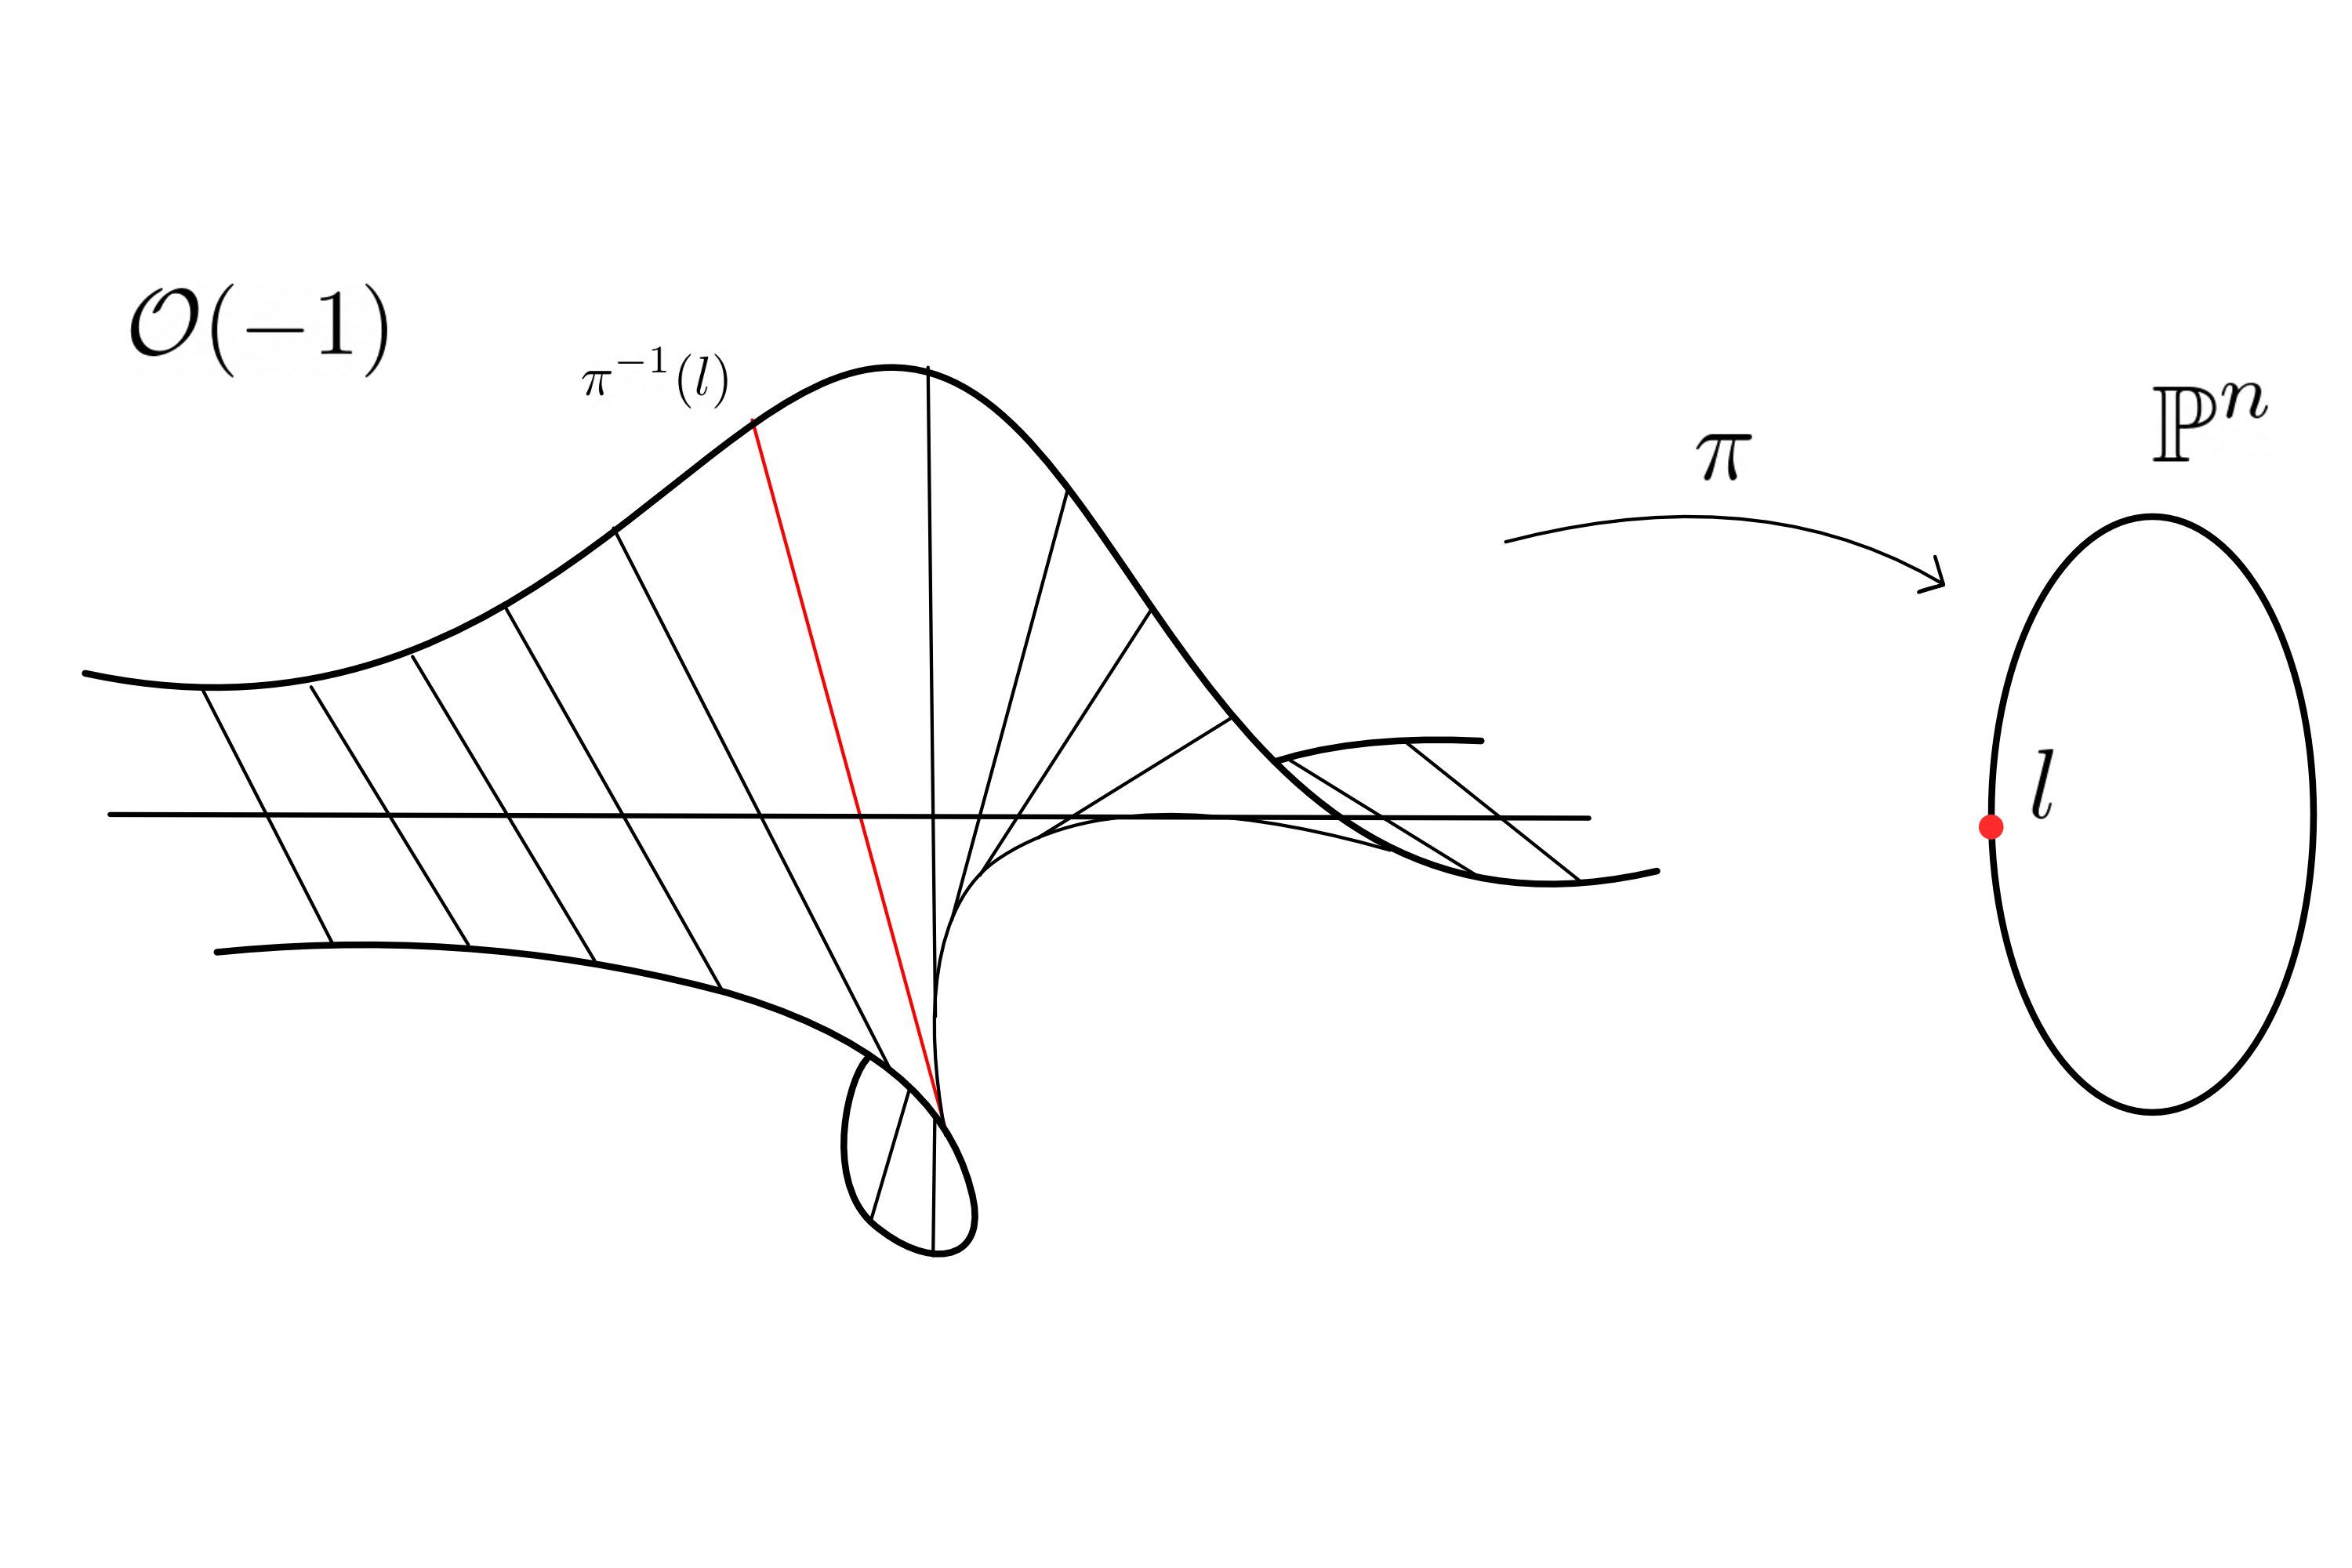
\includegraphics[width=0.7\linewidth]{Imagenes/tautologico}
		\caption{Interpretación geométrica del haz lineal $\mathcal{O}(-1)$.}
		\label{fig:tautologico}
	\end{figure}
	
	
	\begin{definition}
		Consideremos el haz lineal $\oo(-1)$ sobre el espacio proyectivo $\pp^n$.
		\begin{enumerate}
			\item El haz lineal $\mathcal{O}(-1)$ es llamado \textbf{haz tautológico}.
			\item El haz dual $\mathcal{O}(1):=\mathcal{O}(-1)^*$ es llamado \textbf{haz de hiperplanos}.
			\item El haz trivial sobre $\pp^n$ lo denotamos como $\mathcal{O}(0):=\pp^n\times\cc$.
			\item La potencia tensorial la denotamos como $\mathcal{O}(-d):=\mathcal{O}(-1)^d$ y  $\mathcal{O}(d):=\mathcal{O}(1)^{d}$.
		\end{enumerate}
	\end{definition}

	\begin{lemma}\label{seccionesnotriviales}
		Sea $L$ un haz lineal holomorfo sobre una variedad compleja conexa compacta $M$. Entonces $L$ es trivial si, y solo si, $L$ y su dual $L^*$ admite secciones globales no triviales.  
	\end{lemma}
	\begin{proof}
		Supongamos que $L$ es trivial. Por el ejemplo \ref{seccionesdeltrivial}, $L$ admite secciones constantes no cero. Además, el dual $L^*$ vuelve a ser $L$, por lo que $L^*$ también admite secciones constantes no cero.
		
		Ahora supongamos que $L$ y $L^*$ admite secciones globales no cero. Tomemos las secciones globales no cero
		\begin{equation*}
			s\in H^0(M,L),
			\qquad
			t\in H^0(M,L^*).
		\end{equation*}
		Entonces por el ejemplo \ref{Ltensordual} tenemos que
		\begin{equation*}
			s\otimes t\in H^0(M,L\otimes L^*)\cong H^0(M,\oo_M).
		\end{equation*}
		Eso significa que $s\otimes t$ corresponde con una función holomorfa global $f\in \oo_M(M)$. Por el teorema \ref{holomorfasglobal}, $s\otimes t$ es constante. 
		
		Como $s$ y $t$ son holomorfas no cero, siempre existe $r\in M$ tal que $s(r)\neq 0$ y $t(r)\neq o$. Con lo cual $(s\otimes t)(r)\neq 0$. De esta manera, $s\otimes t\neq 0$. En particular, $s(p)\neq 0$ para todo punto $p\in M$.
		
		Ahora bien, una sección global que nunca se anula trivializa globalmente al haz $L$. Definamos
		\begin{align*}
			\Psi:M\times \cc\longrightarrow L,\\
			\Psi(p,\lambda)=\lambda s(p).
		\end{align*}
		Consideremos una trivialización local $(U,\psi)$ de $L$, entonces
		\begin{equation*}
			s|_U(p)=(p,f(p)),\qquad \text{para todo }\ p\in U
		\end{equation*}
		donde $f\in\oo_M(U)$. Como $s$ nunca se anula, entonces $f$ tampoco nunca se anula. Además, como $L|_U=\pi^{-1}(U)\cong U\times \cc$, entonces a todo punto $x\in L|_U$ se le asocia de manera única un punto $(q,\lambda')\in U\times \cc$. De esta manera, podemos definir $\Psi^{-1}$ localmente como
		\begin{equation*}
			\Psi|_U^{-1}(x)=\left(q,\frac{\lambda'}{f(q)}\right),
		\end{equation*}
		la cual está bien definida porque $f$ nunca se anula.
		Notemos que en efecto es la inversa, pues
		\begin{align*}
			\Psi\circ\Psi^{-1}(x)=\Psi\left(q,\frac{\lambda'}{f(q)}\right)=\frac{\lambda'}{f(q)}s(q)=\frac{\lambda'}{f(q)}(q,f(q))=\left(q,\frac{\lambda'}{f(q)}f(q)\right)=(q,\lambda')=x,\\
			\Psi^{-1}\circ\Psi(p,\lambda)=\Psi^{-1}(\lambda s(p))=\Psi^{-1}(\lambda(p,f(p)))=\Psi^{-1}(p,\lambda f(p))=\left(p,\frac{\lambda f(p)}{f(p)}\right)=(p,\lambda).
		\end{align*}
		Por lo tanto, $\Psi:M\times \cc\to L$ es un biholomorfismo y $L$ es trivial.
	\end{proof}
	
	Con este lema, podemos probar uno de los resultados más importante de los haces lineales del espacio proyectivo.
	
	\begin{theorem}\label{seccionesproyectivo}
		Consideremos el haz lineal $\oo(1)$ del espacio proyectivo $\pp^n$ y sea $d$ un entero positivo no cero. Entonces se cumple lo siguiente:
		\begin{enumerate}
			\item $H^0(\pp^n, \mathcal{O}(d))\cong \cc[z_0,\cdots,z_n]_{(d)}$
			\item $H^0(\pp^n, \mathcal{O}(0))\cong \cc$
			\item $H^0(\pp^n, \mathcal{O}(-d))\cong\{0\}$
		\end{enumerate}
	\end{theorem}
	\begin{proof} $ $
		\begin{enumerate}
			\item Recordemos que el conjunto $\cc[z_0,\cdots,z_n]_{(d)}$ es el anillo de polinomios homogéneos de grado $d$.
			
			Consideremos la cubierta estandar afín de $\pp^n$
			\begin{equation*}
				\pp^n=\bigcup_{i=0}^n U_i.
			\end{equation*}
			En una intersección $U_j\cap U_k$, las funciones de transición de $\mathcal{O}(-1)$ están dadas por 
			\begin{equation*}
				g_{ij}=\frac{z_j}{z_i}.
			\end{equation*}
			Entonces las funciones de transición de $\mathcal{O}(d)$ son de la forma
			\begin{equation*}
				g'_{ij}=\frac{z_k^d}{z_j^d}.
			\end{equation*}
			Por la observación \ref{seccionlocalholomorfa}, toda sección global $s\in H^0(M,L)$ está determinada por una colección de funciones holomorfas $f_i\in\oo_{\pp^n}(U_i)$ tal que $f_j=\frac{z_k^d}{z_j^d}f_k$ en $U_i\cap U_j$. Consideremos la aplicación cociente
			\begin{align*}
				q:\cc^{n+1}\setminus\{0\}\longrightarrow \pp^n,
			\end{align*}
			entonces el pullback $f'_j=f_j\circ q$ está bien definida y holomorfa cuando $z_j\neq 0$. De la relación
			\begin{equation*}
				z_j^df'_j=z_k^d f'_k
			\end{equation*}
			tenemos que la función
			\begin{equation*}
				F(z):=z_j^df_j([z])
			\end{equation*}
			no depende del índice $j$. Así, $F$ es holomorfa en $\cc^{n+1}\setminus\{0\}$. Por el teorema de Hartog \ref{hartogs}, esta función se extiende holomorfamente a $\cc^{n+1}$. Además, satisface la condición de homogeneidad 
			\begin{equation*}
				F(\lambda z)=(\lambda z_j)^d f_j([\lambda z])=\lambda^d F(z),\qquad \lambda\in\cc^*.
			\end{equation*}
			Al expandir en serie de potencias, esta identidad fuerza que solo aparezcan monomios de grado $d$. 
			Escribiendo
			\begin{equation*}
				F=\sum_\alpha a_\alpha z^\alpha,
			\end{equation*}
			la identidad $ F(\lambda z)=\lambda^dF(z)$ implica que
			\begin{equation*}
				\sum_\alpha a_\alpha \lambda^{|\alpha|}z^\alpha
				=
				\sum_\alpha a_\alpha \lambda^d z^\alpha.
			\end{equation*}
			Por unicidad de la serie de potencias,
			$a_\alpha=0$ si $|\alpha|\neq d$. Con lo cual, $F$ es un polinomio homogéneo de grado $d$.
			
			Consideremos un polinomio $P$ homogéneo de grado $d$, entonces en cada abierto $U_j$ podemos definir
			\begin{equation*}
				f_j([z])=\frac{P(z)}{z_j^d}.
			\end{equation*}
			Esta función es holomofa en $U_j$, y la expresión coincide en las intersecciones pues $P$ es un polinomio homogéneo de grado $d$. Por lo tanto, la colección $\{f_j\}_{j=0}^n$ determina una sección global holomorfa de $\mathcal{O}(d)$.
			
			\item Se sigue del ejemplo \ref{H0deltrivial}.
			
			\item Se sigue del lema \ref{seccionesnotriviales}.
		\end{enumerate}
	\end{proof}
	
\subsection{Aplicación asociada a un haz}


    \begin{definition}[Puntos base]
		Sea $L$ un haz lineal sobre una variedad compleja conexa $M$. El conjunto de \textbf{puntos bases} de $L$ está dado por
		\begin{equation*}
			\mathrm{Bs}(L)=\{p\in M:s(p)=0\text{ para todo }s\in H^0(M,L)\},
		\end{equation*}
		donde $s(p)=0$ signifa que la sección $s$ coincide con la sección cero $s_0\in H^0(L,M)$ en el punto $p$.
	\end{definition}

	\begin{remark}
		Sea $L$ un haz lineal sobre una variedad compleja conexa $M$. Para cada sección global $ s\in H^0(M,L) $, su conjunto de ceros
		\begin{equation*}
			Z(s)=\{p\in M: s(p)=0\}
		\end{equation*}
		es un subconjunto cerrado de $M$. En efecto, localmente $L$ se trivializa, y bajo una trivialización $s$ se identifica con una función 
		holomorfa. Por definición,
		\begin{equation*}
			\mathrm{Bs}(L)=\bigcap_{s\in H^0(M,L)} Z(s).
		\end{equation*}
		La intersección arbitraria de cerrados es cerrada, entonces $\mathrm{Bs}(L)\subset M$ es un subconjunto cerrado.\\
		De esta manera, el abierto
		\begin{equation*}
			U:=M\setminus \mathrm{Bs}(L).
		\end{equation*}
		es una variedad compleja por ser un abierto de una variedad compleja.
%		Por definición de $ \mathrm{Bs}(L) $, para todo $ p\in U $ existe al menos una sección global $ s\in H^0(M,L) $ tal que $ s(p)\neq 0 $. Como $s$ es holomorfa, por el teorema de la identidad (\ref{teoidentidad}) el conjunto $ U_s:=\{q\in M \mid s(q)\neq 0\} $ es un abierto de $M$, y contiene a $p$. En particular, $ U_s $ es un abierto de una variedad compleja, luego es una variedad compleja también. Además,
%		\begin{equation*}
%			U=\bigcup_{s\in H^0(M,L)} U_s,
%		\end{equation*}
%		es decir, $ U $ es una unión de variedades complejas de la misma dimensión. Por la proposición (falta cita) $U$ es una variedad compleja.

	\end{remark}

	\begin{propo}
		Sea $L$ un haz lineal holomorfo sobre una variedad compleja $M$ y supongamos que $s_0,\dots,s_N$ es una base de $H^0(M,L)$. Entonces
		\begin{align*}
			\varphi_L:M\setminus Bs(L)\longrightarrow \pp^N\\
			p\mapsto [s_0(p):\cdots:s_N(p)]
		\end{align*}
		es una aplicación holomorfa.
	\end{propo}
	\begin{proof}
		Primero vamos a explicar la definición de $\varphi_L$. 
%		Puntualmente, consideremos $x\in M$, entonces $s_i(x)\in L_x\cong \cc$. Por lo que, $s_i(x)$ determina un punto $p_i\in\cc$. De esta manera, 
%		\begin{equation*}
%			\varphi_L(p)=[p_0:\cdots:p_N].
%		\end{equation*} 
%		Si $p\not\in Bs(L)$, entonces $\varphi_L(p)$ determina un punto bien definido en $\pp^N$.
%		
		Consideremos $p\in M\setminus Bs(L)$ y $\psi:L|_U\cong U\times\cc$ es una trivialización local en una vecindad $U$ de $p$. Además en las fibras, $\psi|_{L_p}:L_p\cong \{p\}\times \cc$. Entonces la notación $\varphi_L(x)=[s_0(p):\cdots:s_N(p)]$ denota al punto
		\begin{equation*}
			[\psi(s_0(p)):\cdots:\psi(s_N(p))]\in\pp^N.
		\end{equation*}	
		Esta definición es independiente de la trivialización, pues cualquier otra trivialización en $U$ es de la forma $f\psi$ para alguna función $f:U\to\cc$ holomorfa. Entonces
		\begin{equation*}
			[f(p)\psi(s_0(p)):\cdots:f(p)\psi(s_N(p))]=[\psi(s_0(p)):\cdots:\psi(s_N(p))].
		\end{equation*}
		Esta descripción local prueba que $\varphi_L$ está bien definida y es holomorfa en $M\setminus Bs(L)$.
	\end{proof}
    
    \begin{remark}
    	La aplicación $\varphi_L$ depende de la base, pero dos elecciones de base inducen aplicaciones que difieren por una tranformación lineal de $\pp^N$. Más aún, podemos definir esta aplicación mediante
    	\begin{align*}
    		\varphi_L:M\setminus \mathrm{Bs}(L)\longrightarrow\pp(H^0(M,L)^*)
    	\end{align*} 
    	el cual asocia a $x\in M\setminus \mathrm{Bs}(L)$ el funcional lineal $H^0(M,L)\to \cc$, $s\mapsto s(x)\in L_x\cong\cc$. Este funcional depende del isomorfismo $L_x\cong\cc$, por lo que obtenemos un punto en $\pp(H^0(M,L)^*)$. Ambas decripciones son compatibles al de fijar una base de $H^0(M,L)$ y coinciden a travez del isomorfismo inducido $\pp(H^0(M,L)^*)\cong\pp^N$.
    \end{remark}

	De este modo, los haces lineales nos sirven para generar coordenadas homogéneas sobre las variedades complejas. Sin embargo, no todo haz nos proporciona suficientes secciones \enquote{bien comportadas} para que la variedad no se \enquote{aplane} o colapse al ser proyectada. Por ello, es natural introducir una noción que defina cuando el haz tiene una \enquote{amplitud} suficiente para generar coordenadas suficientemente ricas.
	
	\begin{definition} 
		Sea $L$ un haz lineal holomorfo sobre una variedad compleja $M$. Decimos que $L$ es un \textbf{haz lineal muy amplio} si la aplicación inducida $\varphi_L$ es un encaje holomorfo.\\
		Decimos que $L$ es un \textbf{haz lineal amplio} si existe $k>0$ tal que la potencia tensorial $L^k$ es un haz lineal muy amplio.
	\end{definition}
	
%	La construcción anterior muestra que las secciones globales de un haz lineal generan de manera natural una aplicación al espacio proyectivo. Cuando dichas secciones son suficientemente abundantes para separar puntos y direcciones tangentes, esta aplicación resulta ser un encaje holomorfo. La noción de haz muy amplio abstrae precisamente esta propiedad y permite caracterizar las variedades proyectivas en términos intrínsecos.
	
	Si una variedad compleja $M$ admite la existencia de un haz lineal amplio, por definición, existe un encaje holomorfo a un espacio proyectivo. Por el teorema (\ref{encajesubvariedades}), $M$ es un biholomorfa a una subvariedad compleja del espacio proyectivo, es decir, $M$ es proyectiva. Vamos a ver que el reciproco también es cierto.

	\begin{theorem}\label{proyectivossiamplio}
		Una variedad compleja conexa compacta es proyectiva si, y solo si, admite un haz lineal amplio.
	\end{theorem}
	\begin{proof}
		Si $L$ es amplio, entonces existe $k>0$ tal que $L^k$ es muy amplio. Entonces la aplicación inducida 
		\begin{equation*}
			\varphi_{L^k}:M\longrightarrow \pp^N
		\end{equation*}
		es un encaje holomorfo. Por la proposición \ref{encajesubvariedades}, $M$ es biholomorfa a una subvariedad compleja de $\pp^N$, es decir, $M$ es proyectiva.
		
		
		Ahora, supongamos que $M$ es una variedad compleja conexa compacta proyectiva. Entonces existe un encaje holomorfo
		\begin{equation*}
			f:M\longrightarrow\pp^N
		\end{equation*}
		Escribamos las coordenadas $f(p)=[p_0:\cdots:p_N]$ para todo $p\in M$.
		
		Consideremos el haz de hiperplanos $\oo(1)$ sobre $\pp^N$ y tomemos la base $z_0,\dots,z_N\in H^0(\pp^N,\oo(1))$. Bajo el isomorfismo del teorema \ref{seccionesproyectivo}, los polinomios lineales $z_0,\dots,z_N$ corresponden con una base de $H^0(\pp^N,\oo(1))$. Por el ejemplo \ref{seccionespullback}, determinan secciones globales del haz pullback
		\begin{equation*}
			s_i=f^*z_i,\qquad i=0,1,\cdots, N.
		\end{equation*}
		Sea $L=f^*\oo(1)$. Consideremos $p\in Bs(L)$, entonces
		\begin{equation*}
			s_i(p)=f^*z_i(p)=0.
		\end{equation*}
		Así,
		\begin{equation*}
			z_i(f(p))=p_i=0,\qquad i=0,1,\cdots, N.
		\end{equation*}
		Por lo que, $Bs(L)=\emptyset$. Luego, 
		\begin{align*}
			\varphi_L(p)&=(s_0(p),\dots,s_N(p))\\
			&=[z_0(f(p)):\cdots:z_N(f(p))]\\
			&=[p_0:\cdots:p_N]\\
			&=f(p).
		\end{align*}
		De esta forma, la aplicación $\varphi_L$ coincide con la aplicación $f$. Por lo tanto, como $f$ es un encaje, entonces $L=f^*\oo(1)$ es un haz muy amplio sobre $M$.
	\end{proof}
    
	\begin{example}[Encaje de Veronese]
		Consideremos el espacio proyectivo $\pp^n$ y el haz lineal $\oo(d)$. Por el teorema \ref{seccionesproyectivo}, las secciones globales de $\oo(d)$ corresponde con los polinomios homogéneos de grado $d$. Escojamos una base de $H^0(\pp^n,\oo(d))$ dada por los monomios de grado $d$
		\begin{equation*}
			z_0^{i_0}\cdots z_n^{i_n},\qquad\text{tal que}\qquad i_0+\cdots+i_n=d.
		\end{equation*}
		Notemos que el número de monomios de grado $d$ es $\binom{d+n}{d}$. Denotamos $N=\dim H^0(\pp^n,\oo(d))-1=\binom{d+n}{d}-1$.
		De esta manera, la aplicación inducida $\varphi_{\oo(d)}:\pp^n\longrightarrow \pp^N$, denotada por $\nu_d$, está dada por
		\begin{equation*}
			[z_0:\cdots:z_n]\mapsto [z_0^d:\cdots:z_0^{i_o}\cdots z_n^{i_n}:\cdots:z_n^d]=[z^\alpha]_{|\alpha|=d}.
		\end{equation*}
		Por su descripción por polinomios homogéneos, $\nu_d$ está bien definida y es holomorfa. 
		Notemos además que $Bs(\oo(d))=\emptyset$, pues si $p=[w_0:\cdots:w_n]$ se anula en todos los monomios $z_i^d$, entonces $w=(0,\dots,0)$. 
		
		Fijemos $i\in\{0,1,\dots,n\}$ y consideremos la carta afín $U_i=Z(z_i)^c\subset \pp^n$. En esta carta, las coordenadas están dadas por
		\begin{equation*}
			u_j=\frac{z_j}{z_i},\qquad j\neq i.
		\end{equation*}
		Consideremos la carta afín del espacio proyectivo 
		\begin{equation*}
			V_i=Z(Y_{de_i})^c\subset\pp^N
		\end{equation*}
		donde $Y_{de_i}$\footnote{En general, las coordenadas $Y_\alpha=z^\alpha$ están indexadas por el multiíndice $\alpha=(\alpha_0,\dots \alpha_n)\in\nn^{n+1}$, donde $e_i$ denota el $i$-ésimo vector de la base canónica.} corresponde con la coordenada $z_i^d$. De esta manera, la aplicación $v_d$ queda dada en coordenadas afines como
		\begin{align*}
			&\cc^n\longrightarrow \cc^N\\
			(u_0,u_1,\dots,u_{j-1},&u_{j+1},\dots,u_n)\mapsto (u^\alpha)_{|\alpha|=d}.
		\end{align*}
		Notemos que esta aplicación tiene inversa localmente pues podemos recuperar las coordenadas originales mediantes
		\begin{equation*}
			\frac{Y_{(d-1)e_i+e_j}}{Y_{de_i}}=\frac{x_i^{d-1}x_j}{x_i}=\frac{x_j}{x_i}=u_j.
		\end{equation*}
		Por lo que, la restricción
		\begin{equation*}
			\nu_d|_{U_i}:U_i\longrightarrow \nu_d(\pp^n)\cap V_i
		\end{equation*}
		es un biholomorfismo. 
		Como las cartas $U_i$ cubren $\pp^n$, se sigue que $\nu_d$ es localmente un biholomorfismo sobre su imagen. Además, la aplicación es inyectiva, pues las coordenadas afines $ \frac{z_j}{z_i}$ pueden recuperarse de manera única a partir de las coordenadas homogéneas de $\nu_d([z])$.
		
		Por ejemplo, consideremos el caso de $\pp^1$ y $d=3$, entonces
		\begin{align*}
			&\nu_3:\pp^1\longrightarrow \pp^3\\
			[s:t]&\mapsto [s^3:s^2t:st^2:t^3].
		\end{align*}
		Definamos
		\begin{equation*}
			Y_{(3,0)}=s^3,\qquad Y_{(2,1)}=s^2t,\qquad Y_{(1,2)}=st^2,\qquad Y_{(0,3)}=t^3.
		\end{equation*}
		Entonces se cumplen las siguientes relaciones
		\begin{align*}
			Y_{(3,0)}Y_{(1,2)}=(s^3)(st^2)=(s^2t)^2&=Y_{(2,1)}^2\\
			Y_{(2,1)}Y_{(0,3)}=(s^2t)(t^3)=(st^2)^2&=Y_{(1.2)}^2\\
			Y_{(3,0)}Y_{(0,3)}=(s^3)(t^3)=(s^2t)(st^2)&=Y_{(2,1)}Y_{(1,2)}.
		\end{align*}
		Por lo que se satisfacen las siguientes ecuaciones
		\begin{align*}
			Y_{(3,0)}Y_{(1.2)}-Y_{(2,1)}^2&=0\\
			Y_{(2,1)}Y_{(0,3)}-Y_{(1,2)}^2&=0\\
			Y_{(3,0)}Y_{(0,3)}-Y_{(2,1)}Y_{(1,2)}&=0,
		\end{align*}
		Así, la imagen de $\nu_3$ está dada por la variedad algebraica
		\begin{equation*}
			\nu_d(\pp^1)=Z(Y_{(3,0)}Y_{(1.2)}-Y_{(2,1)}^2,Y_{(2,1)}Y_{(0,3)}-Y_{(1.2)}^2,Y_{(3,0)}Y_{(0,3)}-Y_{(2,1)}Y_{(1,2)}).
		\end{equation*}
		A esta variedad $\nu_d(\pp^1)$ se le llama \textbf{curva racional}. En general, la imagen de $\nu_d(\pp^n)$ es una variedad algebraica de $\pp^N$ llamada \textbf{variedad de Veronese}.
		\begin{figure}[H]
			\centering
			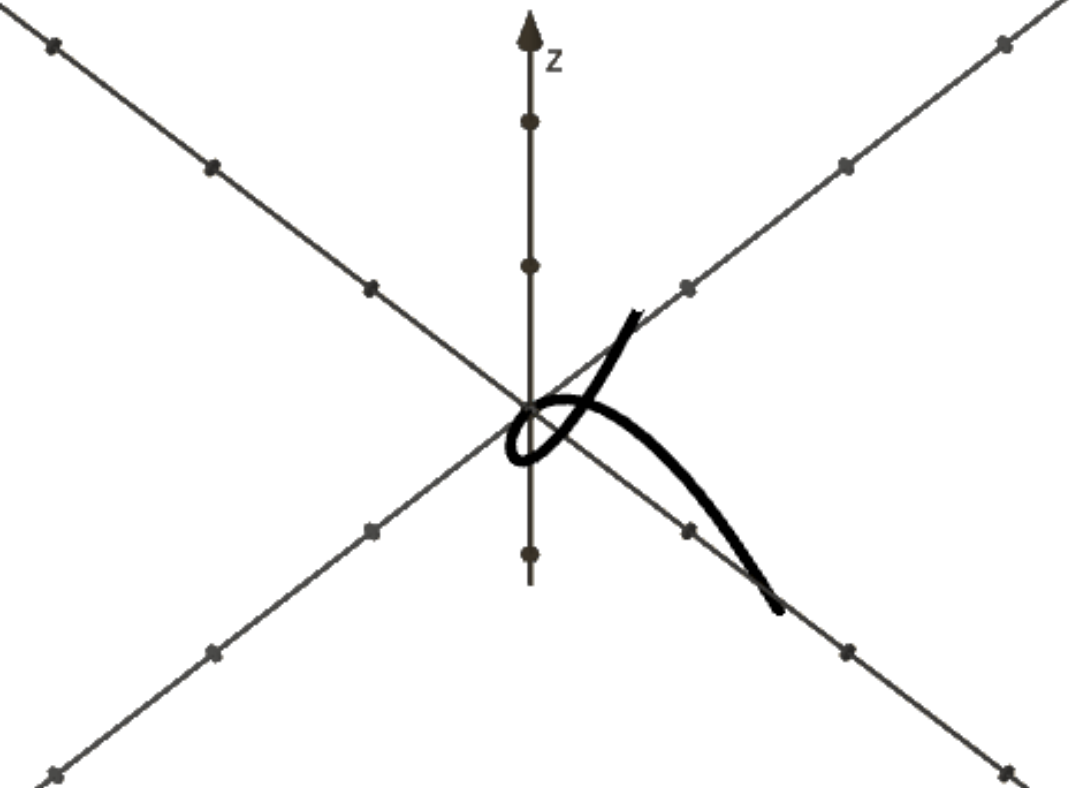
\includegraphics[width=0.3\linewidth]{Imagenes/curva normal}
			\caption{Curva racional en la carta afín $U_0$ dada por $t\mapsto (t,t^2,t^3)$.}
			\label{fig:curva-normal}
		\end{figure}
	
		Por el teorema \ref{encajesubvariedades}, la aplicación $\nu_d=\varphi_{\oo(d)}$ es un encaje holomorfo llamado \textbf{encaje de Veronese}. Por lo tanto, el haz lineal $\oo(d)$ es un haz lineal muy amplio. En particular, el haz lineal $\oo(1)$ es un haz amplio de $\pp^n$. 
	\end{example}
	
	%-----------------------new page----------------------------
	
%	\chapter{Algebrización de Variedades Complejas}

	Hasta este punto hemos introducido diversas herramientas cuya motivación está dada por la pregunta: ¿cuándo puede una variedad compleja describirse mediante ecuaciones algebraicas?
	
	\begin{definition}
		Una variedad compleja se dice \textbf{algebrizable}, o se dice que \textbf{admite una estructura algebraica}, si es biholomorfa a una variedad algebraica $V\subset \pp^N$.
	\end{definition}
	
	Si $M$ es una variedad compleja algebrizable, a la variedad algebraica $V\subset \pp^N$ se le denomina \textbf{realización} de $M$\footnote{También se suele decir que $M$ se \textbf{realiza} como la variedad algebraica $V$.}. Por el Teorema \ref{varalg}, toda variedad algebraica es conexa y compacta; y en consecuencia, en todo este trabajo nos hemos enfocado principalmente en variedades complejas con estas propiedades topológicas, pues toda variedad compleja algebrizable necesariamente debe ser conexa y compacta.
	
	En este último capítulo retomaremos todas las herramientas introducidas anteriormente para darle sentido a la pregunta de algebrización y exponer los criterios que nos permiten determinar cuándo una variedad compleja admite una estructura algebraica.

    \section{Subvariedades Analíticas}
    
    Antes de estudiar la algebrización de variedades, debemos introducir los últimos objetos fundamentales del trabajo.
    
    \begin{definition}[Subconjunto analítico]
    	Sea $M$ una variedad compleja. Un \textbf{subconjunto analítico} de $M$ es un subconjunto cerrado $V\subset M$ con la siguiente propiedad: para cada punto $x\in V$ existe una vecindad $U\subset M$ de $x$ tal que
    	\begin{equation*}
    		U\cap V=\{z\in U:f_1(z)=\cdots=f_k(z)=0\}
    	\end{equation*}  
    	para algunas funciones holomorfas $f_1,\dots,f_k\in\oo_M(U)$.
    \end{definition}
    
    Todo conjuntos algebraico de $\cc$ o $\pp^n$ son subconjuntos analíticos. Así, los subconjuntos analíticos son una generalización de los conjuntos algebraicos para otras variedades complejas.
    
    \begin{definition}[No singular]
    	Sea $M$ una variedad compleja y $V$ un subconjunto analítico de $M$. Decimos que $x\in V$ es \textbf{regular} o \textbf{no singular} si existe una carta $(U,\varphi)$ de $M$ alrededor de $x$ tal que $U\cap V=Z(f_1,\dots,f_k)$ y $\varphi(x)\in \varphi(U)$ es un punto regular de la aplicación
    	\begin{equation*}
    		f:=(f_1\circ\varphi^{-1},\dots,f_k\circ\varphi^{-1}):\varphi(U)\longrightarrow \cc^k.
    	\end{equation*}
    	Es decir, la jacobiana de $f$ en $\varphi(x)$ tiene rango $k$. Denotamos por $V^*$ al conjunto de todos los puntos regulares de $V$.
    	
    	Los puntos del conjunto $V_s:=V\setminus V^*$ son llamados \textbf{puntos singulares}. Por último, decimos que $V$ es \textbf{no singular} si $V_s=\emptyset$, es decir, si $V$ es una subvariedad compleja de $M$ (véase observación \ref{subvariedadesporecuaciones}).
    \end{definition}
    
    Los subconjuntos analíticos pueden interpretarse como variedades complejas que permiten singularidades. Aunque estas singularidades serán solo un subconjunto cerrado y al igual que las variedades algebraicas, los puntos regulares formarán un subconjunto denso. Esto implica que las subvariedades analíticas se comportan como subvariedades complejas con una muy pequeña cantidad de singularidades.
    
    \begin{propo}\parencite[Chap 0, Sec. 2.2]{griffiths}\label{puntossingulares}
    	Sea $M$ una variedad compleja y $V\subset M$ un subconjunto analítico. Entonces el conjuntos de puntos singulares $V_s$ está contenido en un subconjunto analítico de $M$ no igual a $V$.
    \end{propo} 
%    \begin{proof}
%    	Tomemos $p\in V$ y una vecindad $U$ de $p$ tal que
%    	\begin{equation*}
%    		V\cap U=Z(f_1,\dots, f_r),\qquad f_i\in\oo_M(U).
%    	\end{equation*}
%    	Sea $J(f)$ la matriz jacobiana de la aplicación $f=(f_1,\dots,f_r)$. Definamos
%    	\begin{equation*}
%    		k=\max_{q\in V\cap U}\operatorname{rk} J(f)(q).
%    	\end{equation*}
%    	Entonces el conjunto
%    	\begin{equation*}
%    		W=\{q\in V\cap U:\mathrm{rk}J(f)(q)<k\}
%    	\end{equation*}
%    	está definido por la anulación de todos los menores $k\times k$, por lo que es un subconjunto analítico de $V\cap U$. En particular, $W\neq V\cap U$ pues existe al menos una menor $k\times k$ que no se anula idénticamente en $V\cap U$. De esta manera,
%    	\begin{equation*}
%    		V_s\cap U\subset W.
%    	\end{equation*}
%    	Por lo tanto, $V_s$ está contenido en un subconjunto analítico no igual a $V$.
%    \end{proof}
    
%    \begin{remark}
%    	Sea $V$ un subconjunto analítico de $M$ y $p\in V$ un punto no singular. Por definición, existe una vecindad $U$ de $p$ tal que
%    	\begin{equation*}
%    		V\cap U=Z(f_1,\cdots,f_k)
%    	\end{equation*}
%    	donde la función inducida en una carta tiene rango $k$. En particular, $p$ es un punto regular de $f$ y $f^{-1}(p)=V\cap U$ es una variedad compleja de dimensión $k$ (falta cita). Así, definimos 
%    	\begin{eqnarray*}
%    		\dim_p V:= k.
%    	\end{eqnarray*}
%    \end{remark}
   
    \begin{example}
    	Consideremos $D\subset \cc^n$ un conjunto discreto y cerrado no vacío. Esto significa que para todo punto $p=(p_1,\dots,p_n)\in D$ existe una vecindad del punto $U\subset\cc^n$ tal que
    	\begin{equation*}
    		U\cap D =\{p\}.
    	\end{equation*} 
    	Notemos que $Z(z_1-p_1,\cdots,z_n-p_n)=\{p\}$. Por lo tanto, $D$ es un subconjunto analítico de $\cc^n$.
    \end{example}
    
    \begin{remark}
    	Sabemos que los conjuntos algebraicos de $\mathbb{A}^1_\cc$ solo son conjuntos finitos. Por el ejemplo anterior, cualquier conjunto discreto $D$ en $\cc$ es analítico. Por lo tanto, los conjuntos algebraicos de  $\mathbb{A}^1_\cc$ también son analíticos, pero además, existen subconjuntos analíticos que no son algebraicos (véase ejemplo \ref{graficadelseno}).
    \end{remark}
    
    \begin{lemma}\label{preimagen analitico}
    	Sea $f:N\to M$ una aplicación holomorfa y $V\subset M$ un subconjunto analítico. Entonces $f^{-1}(V)\subset N$ es un subconjunto analítico.
    \end{lemma}
    \begin{proof}
    	Sea $V\subset M$ un subconjunto analítico y definamos $W=f^{-1}(V)$. Consideremos $p\in W$, entonces $f(p)\in V$. Como $V$ es analítico, existe una vecindad $U$ de $f(p)$ tal que
    	\begin{equation*}
    		U\cap V=Z(f_1,\dots,f_k)
    	\end{equation*} 
    	donde $f_1,\dots,f_k\in\oo_M(U)$. Luego, como $f$ es continua, $U'=f^{-1}(U)$ es una vecindad abierta de $p$. Definamos las funciones
    	\begin{equation*}
    		g_i=f_i\circ f:U'\to\cc,\quad i=1,2,\dots,k.
    	\end{equation*}
    	Notemos que las funciones $g_i$ son holomorfas, por ser composición de aplicaciones holomorfas. Así, 
    	\begin{align*}
    		U'\cap W&=f^{-1}(U\cap V)\\
    		&=f^{-1}(Z(f_1,\dots,f_k))\\
    		&=f^{-1}\left(\bigcap_{i=1}^k Z(f_i) \right)\\
    		&= \bigcap_{i=1}^k f^{-1}(Z(f_i))\\
    		&=\bigcap_{i=1}^k Z(f_i\circ f)\\
    		&=\bigcap_{i=1}^k Z(g_i)\\
    		&=Z(g_1,\dots,g_k).
    	\end{align*}
    	Por lo tanto, $W=f^{-1}(V)$ es un subconjunto analítico.
    \end{proof}
    
    \begin{definition}
    	Sea $M$ una variedad compleja y $V$ un subconjunto analítico de $M$. Decimos que $V$ es \textbf{irreducible} si no es posible escribirla como una unión $V=V_1\cup V_2$ de dos subconjuntos analíticos propios $V_i\subset V$ de $M$.\\
    	Un subconjunto analítico irreducible es llamado \textbf{subvariedad analítica}.
    \end{definition}
    
    \begin{corollary}
    	Sea $M$ una variedad compleja y $V$ un subconjunto analítico de $M$. Entonces el conjunto $V^*$ es denso en $V$ y una subvariedad compleja no vacía de $M$.
    \end{corollary}
    \begin{proof}
    	Supongamos que $V$ es irreducible. Sea $p\in V$ un punto regular, entonces existe una vecindad $U$ de $p$ tal que $V\cap U\subset V^*$ es una subvariedad compleja de $U$. De esta manera, $p$ es un punto interior de $V^*$. Con lo cual, $V^*$ es un abierto. 
    	
    	Por la proposición \ref{puntossingulares}, sabemos que existe un subconjunto analítico $W$ tal que
    	\begin{equation*}
    		V_s\subset W\subsetneqq V.
    	\end{equation*}
    	Como $W\neq V$, entonces $V^*=V\setminus V_s$ es no vacío. En particular, $V^*$ es una subvariedad compleja no vacía.
    	
    	Supongamos que $V_s$ contiene un abierto no vacío $A\subset V$. Entonces $A\subset W$. Dado que $V$ es irreducible y $W$ es un subconjunto analítico propio, por el teorema de la identidad, las funciones que definen a $W$ cerca de $A$ se deben anular siempre. Esto implica que $W=V$, lo cual es una contradicción. Con lo cual, $A$ es vacío.
    	
    	Si $V_s$ contuviera un abierto no vacío de $V$, entonces también lo contiene el subconjunto analítico $W$. Sin embargo, un subconjunto analítico propio de un subconjunto analítico irreducible no puede contener un abierto relativo. Por lo que, $V_s$ no contiene abiertos de $V$
    	
    	Como $V_s$ es cerrado en $V$ y no contiene abiertos de $V$, entonces
    	\begin{equation*}
    		\mathrm{Int}(V_s)=\emptyset.
    	\end{equation*}
    	Con lo cual, $V^*=V\setminus V_s$ es denso en $V$.
    	
    	Si $V$ no es irreducible, se aplica el argumento a cada componente irreducible $V_i$. Obteniendo que $V_i^*$ es denso en $V_i$, y por tanto la unión de todos los puntos regulares es densa en $V$.
    \end{proof}
    
    \begin{definition}
    	Sea $V\subset M$ una subvariedad analítica. Definimos la \textbf{dimensión} de $V\subset M$ como
    	\begin{equation*}
    		\dim V:=\dim V^*.
    	\end{equation*}
    	Es decir, la dimensión como subvariedad compleja de sus puntos no singulares.
    	
    	De igual manera, definimos la \textbf{codimensión} de $V$ como la codimensión de $V^*$.
    	Una \textbf{hipersuperficie analítica} es una subvariedad analítica de codimensión uno.
    \end{definition}
    
    \begin{remark}
    	Una consecuencia directa de la geometría local (véase proposición \ref{hipersuperficiesenCn}), es que toda hipersuperficie analítica en una variedad compleja $M$ está definida localmente como el conjunto de ceros de una sola función. Es decir, si $H\subset M$ es una hipersuperficie analítica, entonces para todo punto $p\in H$ existe una vecindad $U$ de $p$ y una función holomorfa $f\in \oo_M(U)$ irreducible tal que
    	\begin{equation*}
    		H\cap U=Z(f).
    	\end{equation*}
    \end{remark}
    
    \begin{example}
    	Consideremos la función holomorfa $y^2-x^2-x^3$ en $\cc^2$. Su conjunto de ceros es un subconjunto analítico en $\cc^2$, y de hecho es irreducible, por lo que
    	\begin{equation*}
    		Z(y^2-x^2-x^3)\subset\cc^2
    	\end{equation*}
    	es una subvariedad analítica irreducible (de hecho también algebraica) de $\cc^2$. En una vecindad suficientemente pequeña del origen, la función $\sqrt{1+x}$ es holomorfa. De esta manera, como
    	\begin{equation*}
    		y^2-x^2-x^3=(y-x\sqrt{1+x})(y+x\sqrt{1+x}),
    	\end{equation*}
    	el germen de la subvariedad es reducible. Por lo tanto, existen dos componentes irreducibles localmente definidas por los factores $y\pm x\sqrt{1+x}$.
    	\begin{figure}[H]
    		\centering
    		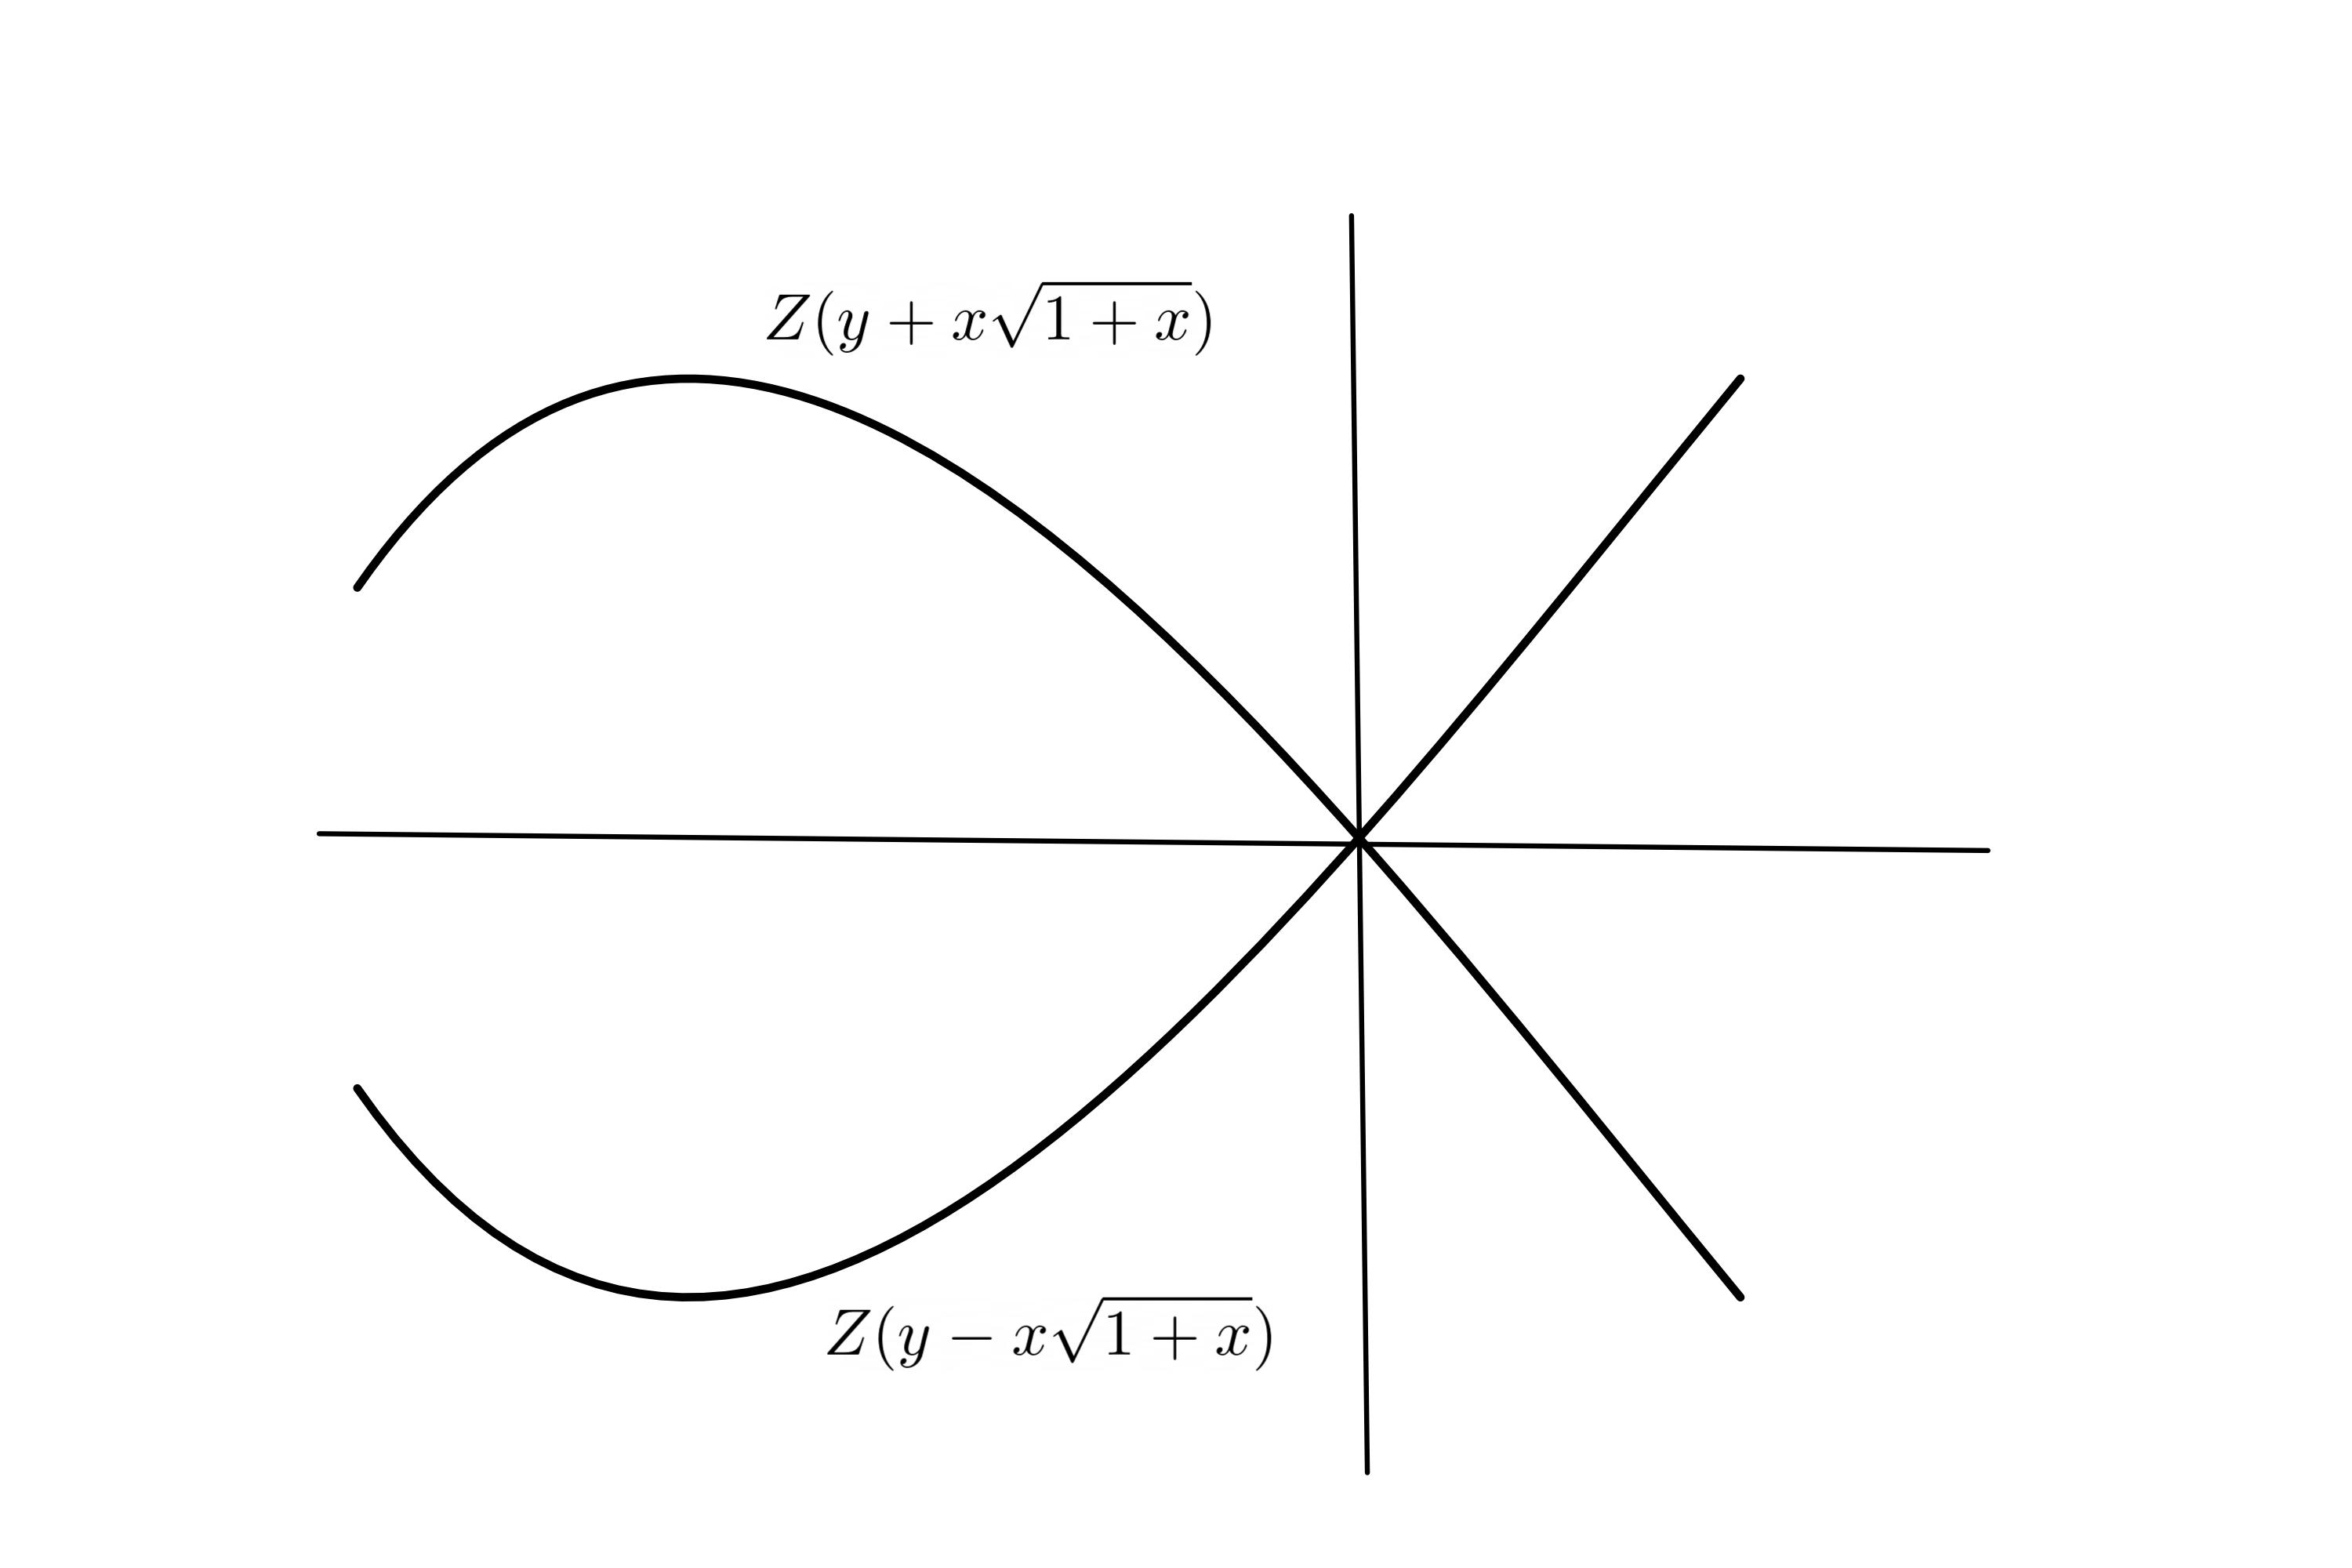
\includegraphics[width=0.5\linewidth]{Imagenes/componenteslocales}
    		\caption{Componentes irreducibles locales de $Z(y^2-x^2-x^3)$.}
    		\label{fig:componenteslocales}
    	\end{figure}
    	
    \end{example}
    
    Por último, presentaremos uno de los resultados más importantes de las subvariedades analíticas:
    
    \begin{theorem}\parencite[Chap 0, Sec. 2.2]{griffiths}\label{irreducibleconexo}
    	Sea $M$ una variedad compleja y $V\subset M$ un subconjunto analítico. Entonces $V$ es irreducible si, y solo si, $V^*$ es conexa.
    \end{theorem}
	
    \subsection{Teoremas de Remmert}
		
		Los subconjuntos analíticos son objetos muy importantes en la geometría algebraica y el análisis complejo. Sin embargo, describir su comportamiento es una tarea lejos de ser trivial y llevó a muchos matemáticos a estudiar en profundidad estos objetos.
		
		Los teoremas de \textit{Remmert} describen el comportamiento de los subconjuntos analíticos bajo imágenes y cerradura. El \textit{teorema de la aplicación propia} nos garantiza que la imagen de un subconjunto analítico por una aplicación holomorfa propia es nuevamente un subconjunto analítico, mientras que el \textit{teorema de Remmert-Stein} describe las condiciones para que la cerradura de un subconjunto analítico siga siendo analítico.
		
		Estos resultados son importantes para la teoría de subconjuntos analíticos y funcionan como herramientas esenciales en nuestro entendimiento de los encajes de variedades complejas. Solo nos limitaremos a enunciar ambos teoremas, remitiendo al lector a las referencias clásicas para entender sus demostraciones (véase \parencite{griffiths}, \parencite{lojasiewicz} y \parencite{chirka}). 
		
    	\begin{theorem}[de la aplicación propia de Remmert]\label{aplicacionpropia}
    		Sea $f:M\to N$ una aplicación holomorfa propia\footnote{Recordemos que una aplicación propia es una función continua entre espacios topológicos cuya preimagen de conjuntos compactos es compacta.} entre variedades complejas. Si $V$ es un subconjunto analítico de $M$, entonces $f(V)$ es un subconjunto analítico de $N$.
    	\end{theorem}
    	Una demostración puede consultarse en el libro \parencite[Chap.3~,Sec.2]{griffiths}, donde se basa fuertemente en una versión particular del teorema de Remmert-Stein llamado \textbf{teorema de Extensión de Levi (II)} y muchas técnicas del análisis complejo. Otra demostración, de carácter más geométrico, fue dada por Chirka \parencite[Chap. 4~, Sec.4.4]{chirka}.
    	
		
		\begin{theorem}[de Remmert-Stein para variedades complejas]\label{remmertstein}
			Sea $M$ una variedad compleja conexa de dimensión $n$ y $Z\subset M$ un subconjunto analítico de codimensión menor a $k+1$. Si $V\subset M\setminus Z$ es un subconjunto analítico de codimensión $k$, entonces la cerradura $\overline{V}$ en $M$ es un subconjunto analítico. 
		\end{theorem}
		
		Para probar este teorema se hace una reducción local del mismo. En primer lugar, por la proposición \ref{puntossingulares}, el conjunto de puntos singulares de $Z$ está contenido en un subconjunto analítico propio $Z_1$. Asimismo, los puntos singulares de $Z_1$ están contenidos en un subconjunto analítico propio $Z_2\subset Z_1$. De esta manera, tenemos la siguiente cadena de subconjuntos analíticos
		\begin{equation*}
			Z=Z_0\supset Z_1 \supset Z_2 \supset \cdots 
		\end{equation*}
		con cada $Z_j\setminus Z_{j+1}$ una subvariedad compleja de codimensión $\geq k$ en $M$. Como cada $Z_{j+1}$ es un subconjunto analítico propio de $Z_j$, su dimensión es estrictamente menor, por lo tanto, el proceso termina después de un número finito de pasos. Entonces existe un $r\in\nn$ tal que $Z_{r+1}=\emptyset$. De esta manera, podemos extender $V$ sucesivamente en cada subvariedad $Z_{j}\setminus Z_{j+1}$, primero tomando la cerradura en $M\setminus Z_{1}$, luego en $M\setminus Z_2$ y continuando una cantidad finita de veces. Con lo cual, es suficiente probarlo suponiendo que $Z\subset M$ es una subvariedad compleja de codimensión $\geq k$.
		
		En segundo lugar, para probar que $\overline{V}$ es analítico, es suficiente mostrar que lo es en una vecindad para cualquiera de sus puntos. Por lo tanto, podemos suponer que $M$ es un polidisco de $\cc^n$ que contiene al origen y $0\in Z$. Después de un cambio de coordenadas,  podemos ver que la subvariedad $Z$ es de la forma $Z=Z(z_1,z_2,\dots,z_{k+1})$. De esta manera, tenemos la reducción local del teorema:
		
		\begin{propo}
			Sean $D\subset\cc^n$ un polidisco que contiene al origen y $Z=Z(z_1,z_2,\dots,z_{k+1})$. Si $V$ es un subconjunto analítico de $D\setminus Z$ de codimensión $k$, entonces $\overline{V}$ es un subconjunto analítico de $D$.
		\end{propo}
		
		\begin{remark}
			El teorema de Remmert-Stein puede ser visto como una generalización geométrica del teorema de Hartogs. Una versión del teorema de Hartogs nos dice que si $f$ es una función holomorfa en $M\setminus\{p\}$, y $\dim M\geq 2$, entonces $f$ se extiende holomorficamente a toda $M$ (véase \parencite[Chap. 2, Sec. 1, Cor. 2.1.6]{huybrechts2005complex}).
			
			En esta misma situación, la gráfica
			\begin{equation*}
				\Gamma_f=\{(x,f(x)):x\in M\setminus \{p\}\}\subset (M\setminus \{p\})\times \cc,
			\end{equation*}
			es un subconjunto analítico. Así, el teorema de Remmert-Stein nos dice que la cerradura $\overline{\Gamma_f}$ es un subconjunto analítico de $M\times \cc$. En particular, $\overline{\Gamma_f}$ resulta ser la gráfica de una función holomorfa
			\begin{equation*}
				\tilde{f}\in\oo_M(M)
			\end{equation*}
			tal que $\tilde{f}|_{M\setminus\{p\}}=f$. Este es exactamente el mismo resultado que nos da Hartogs. 
		\end{remark}
		
    \section{Teorema de Chow}
    
	Hemos estudiado las subvariedades analíticas y visto muchas propiedades interesantes de ellas. Para el objetivo de buscar la algebrización de variedades complejas, vimos que las imágenes de subvariedades analíticas son analíticas (\ref{aplicacionpropia}). Así, un encaje de una variedad compleja al espacio proyectivo significa tener un biholomorfismo entre la variedad y una subvariedad analítica del espacio proyectivo. Por lo tanto, la última pregunta que nos interesa abordar resulta tanto natural como profunda. ¿Cómo son las subvariedades analíticas del espacio proyectivo?
	
	En 1949, \textit{Wei-Liang Chow} publicó su artículo \enquote{On Compact Complex Analytic Varieties}, en el cual demuestra un profundo resultado conocido actualmente como \textit{teorema de Chow} y responde a las cuestiones más importantes de todo este trabajo. La demostración de este resultado ha tenido una historia y desarrollo muy interesante durante el siglo pasado. El enfoque de Chow fue usar varias técnicas analíticas y topológicas, luego en 1953 Reinhold Remmert y Karl Stein presentaron una demostración más simple desarrollando un resultado relacionado con la cerradura de conjuntos analíticos. Tres años después, en 1956, \textit{Jean Pierre Serre} publicó su famoso artículo \textit{"Géométrie algébrique et géométrie analytique"}, bautizado como \textbf{GAGA}, y presentó una demostración muy elegante usando toda la nueva herramienta de gavillas coherentes que desarrolló en su artículo. En nuestro caso, presentaremos una demostración basada en la construcción de Remmert y Stein.

\begin{theorem}[Teorema de Chow]
	Todo subconjunto analítico del $n$-espacio proyectivo es algebraico.
\end{theorem}
	\begin{proof}\parencite{chirka}
		Sea $X\subset \pp^n$ un subconjunto analítico. Consideremos la proyección usual
		\begin{align*}
			\pi:\cc^{n+1}\setminus\{0\}\longrightarrow \pp^n
		\end{align*}
		Tomando $V_0=\pi^{-1}(X)\subset \cc^{n+1}\setminus\{0\}$, entonces $V_0$ es un subconjunto analítico (\ref{preimagen analitico}) de $\cc^{n+1}\setminus\{0\}$. Por el teorema de Remmert-Stein \ref{remmertstein}, la cerradura 
		\begin{equation*}
			V=\overline{V_0}=V_0\cup\{0\}
		\end{equation*}
		es un subconjunto analítico de $\cc^{n+1}$.\\
		Ahora, observemos que  si $z\in V$, entonces para todo $t\in\cc$ tenemos que $tz\in V$. Esto significa que $V$ es un cono completo.
		
		Como $0\in V$, entonces existe una vecindad $U\subset\cc^{n+1}$ de $0$ y $f_1,\dots,f_k\in\mathscr{O}_{\cc^{n+1}}(U)$ tales que 
		\begin{equation*}
			V\cap U=Z(f_1,\dots,f_k).
		\end{equation*}
		Sea $I=\langle \overline{f_1},\dots,\overline{f_k} \rangle\subset \mathscr{O}_{n+1}$ el ideal de gérmenes. Si $\overline{f}\in I$, entonces $f$ se puede escribir como 
		\begin{equation*}
			f(z)=\sum_{i=0}^{\infty}h_i(z)
		\end{equation*}
		donde $h_i\in\cc[z_0,\dots,z_n]_{(i)}$ son polinomios homogéneos de grado $i$.\\
		Como $V$ es un cono, entonces $\overline{h_i}\in I$ para todo $i$. En efecto, si $z\in V$ y $|\lambda|<1$, entonces 
		\begin{equation*}
			0=f(\lambda z)=\sum_{i=0}^{\infty}h_i(\lambda z)=\sum_{i=0}^{\infty}\lambda^ih_i( z)
		\end{equation*}
		Como $f(\lambda z)$ es holomorfa en $\lambda$, entonces por el teorema de la identidad, $h_i(z)=0$ para todo $i\in\nn$. Con esto, $\overline{h_i}\in I$.\\
		Así, $I$ está generado por polinomios homogéneos. Como $\mathscr{O}_{n+1}$ es noetheriano (véase teorema \ref{anillonoetheriano}), $I$ es finitamente generado. Esto significa que existen $F_1,\dots, F_m\in\cc[z_0,\dots,z_n]$ polinomios homogéneos tal que $I=\langle F_1,\dots, F_m \rangle$.
		Por lo tanto, $X=Z(F_1,\dots,F_m)$.
	\end{proof}
	
	Supongamos que $M$ admite un haz lineal amplio $L\longrightarrow M$, entonces existe un encaje holomorfo a algún espacio proyectivo $\varphi:M\hookrightarrow\pp^N$
	\[\begin{tikzcd}
		L \\
		\\
		M && {\mathbb{P}^N}
		\arrow[no head, from=1-1, to=3-1]
		\arrow[hook, from=3-1, to=3-3]
	\end{tikzcd}\]
	Como $\varphi$ es un encaje, $\varphi(M)$ es biholomorfo a $M$. Por el teorema de la aplicación propia (\ref{aplicacionpropia}), $\varphi(M)\subset\pp^N$ es una subvariedad analítica. Por el teorema de Chow, $\varphi(M)$ es una variedad algebraica. Por lo tanto, podemos concluir que:

\begin{corollary}
	Toda variedad compleja que admite un haz amplio es algebraica.
\end{corollary}

	Como observamos en el capítulo \ref{cap2}, en geometría compleja no existe un resultado general análogo al teorema de Whitney. Por ello, resulta natural buscar encajes en un espacio tan familiar y estructurado como lo es el espacio proyectivo complejo \(\mathbb{P}^N\). Sin embargo, el teorema de Chow nos muestra que la posibilidad de realizar una variedad compleja como subvariedad proyectiva es una propiedad exclusiva de las variedades algebrizables.
	
	En geometría algebraica, una variedad proyectiva se entiende como una subvariedad algebraica del espacio proyectivo. En nuestra definición, toda variedad proyectiva admite un encaje en un espacio proyectivo complejo; por el Teorema \ref{proyectivossiamplio}, dicha variedad es algebraica. Por lo tanto, nuestra definición de variedad proyectiva coincide con la noción clásica de la geometría algebraica.

	\begin{corollary}\label{teoriemann}
		Toda superficie de Riemann compacta es algebraica.
	\end{corollary}
	
	Con ello observamos que toda superficie de Riemann compacta puede realizarse como una variedad algebraica de dimensión $1$, es decir, como una curva algebraica. Sin embargo, estos resultados son solo teórico y no constituyen, por sí mismos, un método directo para determinar ecuaciones explícitas de una variedad compleja. De hecho, existe una rama activa de las matemáticas dedicada precisamente a construir y estudiar ecuaciones asociadas a superficies de Riemann; un ejemplo clásico de esta perspectiva es la teoría de las curvas modulares.
	
	\begin{example}\parencite{curvaselipticas}
		Consideremos la superficie de Riemann
		\[
		T=\cc/\Lambda,
		\]
		donde $\Lambda=\omega_1\zz+\omega_2\zz$ es una retícula de $\cc$. A este retículo le asociamos la \textbf{función de Weierstrass} $\wp$, que desciende a una función meromorfa en $T$ y está dada por
		\[
		\wp(z)=\frac{1}{z^2}+\sum_{\omega\in\Lambda\setminus\{0\}}
		\left(\frac{1}{(z-\omega)^2}-\frac{1}{\omega^2}\right).
		\]
		Su derivada satisface la relación
		\[
		(\wp'(z))^2=4\wp(z)^3-g_2\wp(z)-g_3,
		\]
		donde $g_2$ y $g_3$ son constantes que dependen de $\Lambda$ y vienen dadas por las \textbf{series de Eisenstein}
		\[
		g_2=60\sum_{\omega\in\Lambda\setminus\{0\}}\frac{1}{\omega^4},
		\qquad
		g_3=140\sum_{\omega\in\Lambda\setminus\{0\}}\frac{1}{\omega^6}.
		\]
		Con esto, obtenemos una aplicación holomorfa bien definida
		\[
		\phi:T\longrightarrow \pp^2,\qquad
		z\longmapsto [\wp(z):\wp(z)^2:1],
		\]
		la cual define un encaje holomorfo. Así, se obtiene un biholomorfismo entre el toro $T$ y la curva elíptica dada por la ecuación
		\[
		4y^2=4x^3-g_2x-g_3.
		\]
		En general, se puede probar que toda superficie de Riemann de género $1$ está dada por la ecuación afín
		\begin{equation*}
			y^2=x(x-1)(x-\lambda),\qquad \text{para todo }\ \lambda\in\cc\setminus\{0,1\}. 
		\end{equation*}
	\end{example}

	\begin{example}[Encaje de Segre]
		Consideremos la superficie compleja $M=\pp^1\times\pp^1$ y denotemos por $p_1:M\to \pp^1$ y $p_2:M\to \pp^1$ las proyecciones de $M$. Por el teorema \ref{seccionesproyectivo}, sabemos que
		\begin{equation*}
			H^0(\pp^1,\oo(1))\cong\langle x_0,x_1\rangle, \qquad H^0(\pp^1,\oo(1))\cong\langle y_0,y_1\rangle.
		\end{equation*}
		Además, el pullback de las secciones bajo las proyecciones vuelven a ser los monomios $x_0,x_1,y_0,y_1$. De esta manera, las secciones $x_0$ y $x_1$ son linealmente independientes en $H^0(M,p_1^*\oo(1))$, y análogo con $y_0$ y $y_1$. Por lo que, estas secciones definen un subespacio lineal
		\begin{equation*}
			\cc[x_0,x_1]_{(1)}\otimes \cc[y_0,y_1]_{(1)}=\langle x_0,x_1\rangle\otimes \langle y_0,y_1\rangle\subset H^0(M,p_1^*\oo(1))\otimes H^0(M,p_2^*\oo(1)).
		\end{equation*}
		Definamos el haz lineal $L=p_1^*\oo(1)\otimes p_2^*\oo(1)$. Entonces, las secciones
		\begin{equation*}
			x_0\otimes y_0,\enspace x_0\otimes y_1,\enspace x_1\otimes y_0,\enspace x_1\otimes y_1
		\end{equation*}
		definen secciones linealmente independientes de $H^0(M,L)$. Usando el isomorfismo
		\begin{align*}
			\cc[x_0,x_1]\otimes \cc[y_0,y_1]\cong \cc[x_0,x_1,y_0,y_1]
		\end{align*}
		obtenemos que los productos 
		\begin{equation*}
			x_0y_0,\enspace x_0y_1,\enspace x_1y_0,\enspace x_1y_1
		\end{equation*}
		definen secciones linealmente independientes de $H^0(M,L)$. Con lo cual, obtenemos el morfismo inducido por estas secciones
		\begin{align*}
				&\sigma:\pp^1\times\pp^1\longrightarrow \pp^3\\
			([x_0:x_1],[y_0:&y_1])\mapsto [x_0y_0:x_0y_1:x_1y_0:x_1y_1]
		\end{align*}

		Notemos que la aplicación $\sigma$ es holomorfa, pues sus coordenadas homogéneas son productos de coordenadas homogéneas en cada factor. Para probar que $\sigma$ es un encaje holomorfo, estudiaremos su expresión en cartas afines. Consideremos las cartas estándar de $\pp^1$
		\begin{align*}
			&U_0=\{[x_0:x_1]:x_0\neq 0\},\qquad U_1=\{[x_0:x_1]:x_1\neq 0\},\\
			&V_0=\{[y_0:y_1]:y_0\neq 0\},\qquad V_1=\{[y_0:y_1]:y_1\neq 0\}.
		\end{align*}
		En $U_0\times V_0$ tenemos las coordenadas afines $(s,t)$ donde
		\begin{equation*}
			s=\frac{x_1}{x_0},\qquad t=\frac{y_1}{y_0}.
		\end{equation*}
		Dado que 
		\begin{equation*}
			[x_0y_0:x_0y_1:x_1y_0:x_1y_1]=\left[ 1:\frac{y_1}{y_0}:\frac{x_1}{x_0}:\frac{x_1y_1}{x_0y_0}\right],
		\end{equation*}
		entonces en las coordenadas $(s,t)$ la aplicación $\sigma$ queda dada como
		\begin{equation*}
			(s,t)\longmapsto [1:t:s:st].
		\end{equation*}
		Por tanto, sobre la carta afín $Z(X_0)^c\subset\pp^3$, la inversa de $\sigma$ sobre su imagen viene dada por
		\begin{equation*}
			[X_0:X_1:X_2:X_3]\longmapsto \left([1:X_2/X_0],[1:X_1/X_0]\right),
		\end{equation*}
		la cual es holomorfa. Análogamente, en las otras tres cartas de $M$ se obtienen expresiones locales de $\sigma$ y de su inversa dadas por
		\begin{align*}
			&U_0\times V_1:\quad (s,t)\mapsto [t:1:st:s],\qquad
			[X]\mapsto \left([1:X_3/X_1],[X_0/X_1:1]\right),\\
			&U_1\times V_0:\quad (s,t)\mapsto [s:st:1:t],\qquad
			[X]\mapsto \left([X_0/X_2:1],[1:X_3/X_2]\right),\\
			&U_1\times V_1:\quad (s,t)\mapsto [st:s:t:1],\qquad
			[X]\mapsto \left([X_1/X_3:1],[X_2/X_3:1]\right).
		\end{align*}
		De aquí se sigue que $\sigma$ induce un biholomorfismo entre $M=\pp^1\times\pp^1$ y su imagen.
		
		Más aún, la imagen de $\sigma$ es la variedad algebraica proyectiva
		\begin{equation*}
			\sigma(M)=Z(X_0X_3-X_1X_2).
		\end{equation*}
		De esta manera, por la proposición \ref{encajesubvariedades}, la aplicación $\sigma$ es un encaje holomorfo.
		
		Por lo tanto, la superficie compleja $M=\pp^1\times\pp^1$ es algebrizable y la variedad algebraica asociada es
		\begin{equation*}
			V=Z(X_0X_3-X_1X_2)\subset\pp^3,
		\end{equation*}
			
%			Resta identificar la imagen. Si
%			\[
%			[X_0:X_1:X_2:X_3]=\sigma([u_0:u_1],[v_0:v_1]),
%			\]
%			entonces
%			\[
%			X_0X_3-X_1X_2
%			=
%			(u_0v_0)(u_1v_1)-(u_0v_1)(u_1v_0)=0,
%			\]
%			luego \(\sigma(\PP^1\times \PP^1)\subseteq V(X_0X_3-X_1X_2)\).
%			
%			Recíprocamente, si \([X_0:X_1:X_2:X_3]\in V(X_0X_3-X_1X_2)\), entonces la matriz
%			\[
%			\begin{pmatrix}
%				X_0 & X_1\\
%				X_2 & X_3
%			\end{pmatrix}
%			\]
%			tiene determinante cero, y por tanto rango a lo más uno. En consecuencia, dicha matriz se descompone como producto exterior de dos vectores no nulos de \(\CC^2\), es decir, existen \((u_0,u_1)\neq (0,0)\) y \((v_0,v_1)\neq (0,0)\) tales que
%			\[
%			\begin{pmatrix}
%				X_0 & X_1\\
%				X_2 & X_3
%			\end{pmatrix}
%			=
%			\begin{pmatrix}
%				u_0\\
%				u_1
%			\end{pmatrix}
%			\begin{pmatrix}
%				v_0 & v_1
%			\end{pmatrix}.
%			\]
%			Por lo tanto,
%			\[
%			[X_0:X_1:X_2:X_3]
%			=
%			[u_0v_0:u_0v_1:u_1v_0:u_1v_1]
%			\in \sigma(\PP^1\times\PP^1).
%			\]
%			Así,
%			\[
%			\sigma(\PP^1\times\PP^1)=V().
%			\]
%			

	\end{example}

\section{Otros criterios de algebrización}

En esta última sección presentaremos dos conceptos clave en la geometría compleja: las variedades de Moishezon y las variedades de Kähler. Ambos están profundamente relacionados con el problema de la algebrización. Sin embargo, para estudiarlos detalladamente necesitamos desarrollar herramientas más avanzadas que las desarrolladas hasta ahora.

La teoría de Moishezon se apoya en las funciones y aplicaciones meromorfas, las cuales surgen como un análogo a las funciones racionales y equivalencia birracional de la geometría algebraica. Por otro lado, la teoría de Kähler involucra técnicas de geometría diferencial, como métricas riemannianas, formas diferenciales, formas holomorfas y teorías de cohomología.

El objetivo no es desarrollar en profundidad estas teorías, sino presentar su importancia en la algebrización. Mientras que el trabajo de Moishezon estableció una relación muy profunda entre la geometría compleja con la algebraica, las variedades de Kähler lo hacen desde la geometría diferencial. De esta manera, esta sección funciona como una extensión conceptual del trabajo, orientada a mostrar conexiones con resultados más profundos de la geometría compleja.

\subsection{Variedades de Moishezon}

En geometría diferencial o algebraica, es común estudiar el comportamiento global de los objetos estudiando sus funciones. Sin embargo, notamos que las funciones holomorfas sobre variedades complejas conexas compactas (por ejemplo, las superficies de Riemann compactas) son constantes (\ref{holomorfasglobal}). Por lo que no podemos obtener información global de estas variedades a partir de sus funciones ¿Qué podemos hacer?

Las funciones meromorfas extienden el concepto de funciones holomorfas al permitir \enquote{polos controlados}, lo que enriquece aún más la estructura analítica de las variedades. Más aún, el conjunto de todas las funciones meromorfas forma un campo (véase proposición \ref{campodefunciones}), lo cual permite aplicar herramientas algebraicas más potentes. De esta manera, el estudio de las funciones meromorfas se vuelve esencial para comprender la estructura local y la geometría global de las variedades complejas.

\begin{definition}
	Sea $M$ una variedad compleja y $p\in M$. Definamos
	\begin{equation*}
		\mathcal{K}_{M,p}:=Q(\oo_{M,p})
	\end{equation*}
	donde $Q(\oo_{M,p})$ es el campo de fracciones asociado al dominio entero $\oo_{M,p}$ (véase corolario \ref{dominiolocal}). Esto es,
	\begin{equation*}
		\mathcal{K}_{M,p}=\left\{ \frac{f_p}{g_p}:f_p,g_p\in\oo_{M,p}\text{ y }g_p\neq 0\right\}.
	\end{equation*}
	Este campo es llamado \textbf{campo de funciones meromorfas} en $p$.
\end{definition}  

\begin{definition}
	Sea $M$ una variedad compleja. Una \textbf{función meromorfa} sobre $U\subset M$ es una aplicación
	\begin{equation*}
		f:U\longrightarrow \bigsqcup_{x\in U}\mathcal{K}_{M,x}
	\end{equation*}
	la cual asocia a $x\in U$ una función $f_x\in \mathcal{K}_{M,x}$ la cual cumple que para todo $p\in U$, existe una vecindad $V\subset U$ de $p$ y funciones holomorfas $g,h\in\oo_M(V)$, con $h\neq 0$, tal que $f|_V=\frac{g}{h}$\footnote{Esta igualdad significa que para todo $x\in V$ se tiene que $f(x)=\frac{g_x}{h_x}$.}.
\end{definition}

La \textbf{gavilla de funciones meromorfas} se denota por $\mathcal{K}_{M}$ y asigna a cada abierto $U$ el conjunto de funciones meromorfas sobre $U$.

\begin{propo}\label{campodefunciones}
	Sea $M$ una variedad compleja y $U\subset M$ un abierto conexo. Entonces $\mathcal{K}_{M}(U)$ es un campo.
\end{propo}
\begin{proof}
	Recordemos que la estructura de anillo de $\mathcal{K}_{M}(U)$ está dada punto a punto, es decir,
	\begin{align*}
		(f+g)(x):=f(x)+g(x)\in\mathcal{K}_{M,x}\\
		(fg)(x):=f(x)g(x)\in\mathcal{K}_{M,x}.
	\end{align*}
	y el elemento unidad es la función constante $1$ la cual es la fracción $1/1$ en cada campo $\mathcal{K}_{M,p}$.
	
	Sea $f\in \mathcal{K}_{M}(U)$ no cero. Buscamos un $f^{-1}\in\mathcal{K}_{M}(U)$ tal que $ff^{-1}=1$.
	Como $f\neq 0$, entonces existe un punto $p\in U$ tal que $f_p\in\mathcal{K}_{M,p}$ es no cero. Entonces existe una vecindad $V\subset U$ conexa de $p$ tal que
	\begin{equation*}
		f|_V=\frac gh,\qquad g,h\in\oo_M(V),\enspace h\neq 0,\enspace g_p\not\in\mathfrak{m}_p.
	\end{equation*}
	Es decir, $g_p\neq 0$ como germen en $p$. Notemos que el conjunto 
	\begin{equation*}
		Z=\{x\in V:g(x)=0\}
	\end{equation*}
	es un subconjunto analítico propio, esto es, $g$ no se puede anular en un abierto no vacío de $V$. Si $g$ se anulara en todo $V$, entonces $f|_V=0$ y contradice que $f_p\neq 0$.
	
	De esta manera, podemos definir la inversa localmente 
	\begin{equation*}
		f^{-1}|_V=\frac hg.
	\end{equation*} 
	Repetimos este proceso para cada punto donde el germen no sea nulo. Esto nos da una cubierta $\{W_i\}_{i\in I}$ de $U$ tal que
	\begin{equation*}
		f^{-1}|_{W_i}=\frac{h_i}{g_i}
	\end{equation*}
	está bien definida y satisfacen 
	\begin{equation*}
		f|_{W_i}f^{-1}|_{W_i}=1\in\mathcal{K}_M(W_i).
	\end{equation*}
	Notemos que además las funciones $f^{-1}|_{W_i}$ coinciden en las intersecciones $W_i\cap W_j$. Así, por la propiedad de sección global de la gavilla $\mathcal{K}_M$ tenemos que existe $f^{-1}\in \mathcal{K}_{M}(U)$ tal que
	\begin{equation*}
		ff^{-1}=1.
	\end{equation*}
\end{proof}

Si $M$ es una variedad compleja conexa, el espacio de secciones globales $\mathcal{K}_{M}(M)$ es llamado \textbf{campo de funciones meromorfas} sobre $M$ y lo denotamos por $\mathcal{K}(M)$. Este campo es de suma importancia para las variedades complejas y se relaciona con un teorema muy importante de la geometría compleja.

\begin{theorem}[Siegel]
	Sea $M$ una variedad compleja conexa compacta de dimensión $n$. Entonces
	\begin{equation*}
		\mathrm{trdeg}_\cc\mathcal{K}(M)\leq n.
	\end{equation*}
\end{theorem}
Una demostración detallada puede consultarse en \parencite[Teo. 4.23]{carlosga} y está basado en el lema de Schwarz de análisis complejo.

\begin{definition}
	Sea $M$ una variedad compleja conexa compacta. Definimos la \textbf{dimensión algebraica} de $M$ como
	\begin{equation*}
		a(M):=\mathrm{trdeg}_\cc\mathcal{K}(M).
	\end{equation*}
\end{definition}

Por el teorema de Siegel, la dimensión algebraica siempre está acotada por la dimensión de la variedad. Por lo que, la dimensión algebraica puede interpretarse como una medida del grado en que una variedad compleja se aproxima al mundo algebraico.

\begin{theorem}\parencite[Chap. VIII, Sec. 3.1, Theo. 1]{shafarevich2016basic}
	Sea $V\subset \pp^n$ una variedad algebraica no singular. Entonces las funciones meromorfas y funciones racionales en $V$ coinciden. Es decir, $\mathcal{K}(V)=\cc(V)$.
\end{theorem}

Sabemos que en variedades algebraicas, el grado de trascendencia de $\cc(V)$ coincide con la dimensión de la variedad algebraica (véase observación \ref{dimcubierta}). Así, la dimensión algebraica de una variedad algebraica coincide con su dimensión compleja, esto es,
\begin{equation*}
	a(V)=n.
\end{equation*}
Esto último nos lleva a la siguiente definición.

\begin{definition}
	Una variedad compleja conexa compacta $M$ se llama \textbf{variedad de Moishezon} si
	\begin{equation*}
		a(M)=\dim M.
	\end{equation*}
\end{definition}

Su nombre se debe al matemático ruso \textit{Boris Gershevich Moishezon} y sus trabajos publicados en 1966 \enquote{On $n$-dimensional compact varieties with n algebraically independent meromorphic functions, I, II and III} en los cuales introdujo el estudio de estas variedades y desarrolló los resultados que veremos más adelante.

Las variedades algebraicas son ejemplos de variedades de Moishezon y de esta manera, tenemos el siguiente resultado:

\begin{corollary}
	Toda variedad compleja algebrizable es de Moishezon.
\end{corollary}

De esta manera, ser de Moishezon es una condición necesaria para buscar variedades algebrizables. Así, surgen dos preguntas importantes:

\begin{itemize}
	\item ¿Todas las variedades complejas son de Moishezon?
	\item ¿Ser de Moishezon es una condición suficiente para la algebrización?
\end{itemize}
Sin embargo, las respuestas a estas dos preguntas son negativas. Un contraejemplo a la primera cuestión es el siguiente:

\begin{example}[Variedad que no es Moishezon]\label{hopfsuperficie}
	Sea $A:\cc^2\to\cc^2$ la aplicación definida por
	\begin{equation*}
		A(z_1,z_2)=(\lambda z_1,\lambda z_2),\qquad 0<|\lambda|<1.
	\end{equation*}
	Consideremos el grupo cíclico
	\begin{equation*}
		\langle A\rangle=\{A^n:n\in\zz\}.
	\end{equation*}
	Como $A(z)=\lambda z$, entonces
	\begin{equation*}
		A^n(z)=\lambda^n z.
	\end{equation*}
	Así, tenemos la relación de equivalencia
	\begin{equation*}
		z\sim w\qquad \longleftrightarrow\qquad w=A^n(z)\enspace \text{para algún }\ n\in\zz.
	\end{equation*}
	Con lo cual, obtenemos la superficie compleja
	\begin{equation*}
		M=\cc^2\setminus\{0\}/\sim,
	\end{equation*}
	llamada \textbf{superficie de Hopf} (véase \parencite[Example 1.19]{leecomplex}). En particular, $M$ es difeomorfo a $S^1\times S^3$. Sea
	\begin{equation*}
		f\in\mathcal{K}(M)
	\end{equation*}
	una función meromorfa definida en $M$. Tomando el pullback por el cociente $\pi:\cc^2\setminus\{0\}\to M$
	\begin{equation*}
		\tilde{f}:=f\circ\pi,
	\end{equation*}
	levanta $f$ a una función meromorfa en $\cc^2\setminus\{0\}$ y $A$-invariante, es decir, $\tilde{f}\in\mathcal{K}(\cc^2\setminus\{0\})$ y $\tilde{f}\circ A=\tilde{f}$. Vamos a probar que $\tilde{f}$ es constante.\\
	Notemos que el conjunto $\{0\}$ tiene codimensión $2$ sobre $\cc^2$. Sin embargo, los polos de una función meromorfa están contenidos en un conjunto de codimensión $1$. Así, $\tilde{f}$ tiene una singularidad aislada en el cero. Por el teorema de Hartogs, $\tilde{f}$ se extiende holomorficamente a $0$. En particular, $\tilde{f}$ es continua en $0$.
	Sea $z\in \cc^2\setminus\{0\}$, entonces la sucesión $\{A^nz\}=\{\lambda^nz\}$ converge a cero. Por la continuidad de $\tilde{f}$ en el cero tenemos que 
	\begin{equation*}
		\tilde{f}(z)=\tilde{f}(A^nz)\underset{n\to\infty}{\longrightarrow}\tilde{f}(0).
	\end{equation*}
	Esto quiere decir que $\tilde{f}(z)=\tilde{f}(0)$ para todo $z\in \cc^2\setminus\{0\}$, es decir, $\tilde{f}$ es constante. De esta manera, $f$ es una función constante. Por lo tanto,
	\begin{equation*}
		\mathrm{trdeg}_\cc\mathcal{K}(M)=0.
	\end{equation*} 
	y $M$ no es una variedad de Moishezon.
\end{example}

Un resultado que ya intuía Riemann, el cual fue demostrado más tarde, es que toda superficie de Riemann admite funciones meromorfas no constantes. Es decir, si $S$ es una superficie de Riemann compacta se cumple que
\begin{equation*}
	\mathrm{trdeg}_\cc\mathcal{K}(S)\neq 0.
\end{equation*}
Dado que una superficie de Riemann es una variedad compleja de dimensión $1$, entonces por el teorema de Siegel
\begin{equation*}
	\mathrm{trdeg}_\cc\mathcal{K}(S)=1.
\end{equation*}
De esta manera, toda superficie de Riemann es de Moishezon y por el teorema \ref{teoriemann} sabemos que toda superficie de Riemann compacta es algebrizable. Por lo tanto, en dimensión $1$, ser de Moishezon sí es condición suficiente para ser algebrizable. 

Para dimensión dos, la situación es similar.
\begin{theorem}[Kodaira]
	Toda variedad compleja compacta de dimensión 2 con dos funciones meromorfas algebraicamente independientes es algebrizable.
\end{theorem}  
Por lo tanto, en dimensión $2$, ser de Moishezon también es una condición suficiente para admitir una estructura algebraica. Esto nos quiere decir un contraejemplo de una variedad de Moishezon que no sea algebraica lo vamos a encontrar en dimensión $\geq 3$ (véase contraejemplo de Hironaka \ref{hironakaejemplo}).

Un concepto relacionado con las funciones racionales de variedades algebraicas son las aplicaciones birracionales. Vamos a extender esta área de la geometría algebraica a un contexto analítico.

\begin{definition}[Modificación]
	Sea $\Phi:M\to N$ una aplicación holomorfa propia sobreyectiva. Decimos que $\Phi$ es una \textbf{modificación} (propia) si existen dos subconjuntos analíticos $A\subset M$ y $B\subset N$ tales que 
	\begin{enumerate}
		\item $B=\Phi(A)$.
		\item $\Phi|_{M\setminus A}:M\setminus A\to N\setminus B$ es un biholomorfismo. 
		\item $A$ y $B$ tiene codimensión al menos $1$.
		\item $A$ y $B$ son mínimos con las propiedades anteriores.
	\end{enumerate}
	$A$ es llamado \textbf{conjunto excepcional} y $B$ el \textbf{centro} de la aplicación $\Phi$. También se suele decir que $\Phi$ es el \textbf{blow-down} de $X$ a lo largo de $A$.
\end{definition}

Un modificación propia es el análogo de los morfismos birracionales	 propios de geometría algebraica, pues funcionan como un biholomorfismo en \enquote{casi todas partes}. Es decir, existe un subconjunto analítico cerrado y de interior vacío sobre el cual la aplicación deja de ser un biholomorfismo, pero fuera de él, los espacios son localmente idénticos. En particular, la composición de estos morfismos está bien definidos en un conjunto denso.

\begin{example}[Blow up]
	Vamos a considerar el caso del origen en $\cc^n$. Cada punto $z\in \cc^n$ determina una única línea que pasa por el origen, y en consecuencia un punto en $\pp^{n-1}$, excepto cuando $z=0$. De esta manera, se define
	\begin{equation*}
		\mathrm{Bl}_0\cc^n=\{(z,l)\in\cc^n\times\pp^{n-1}:z\text{ pertenece a la línea }l\subset\cc^n\}.
	\end{equation*}
	Notemos que es exactamente la misma definición que el espacio total del haz tautológico de $\pp^{n-1}$ pero ahora vamos a considerar la proyección a la primera entrada.	
	
	Decimos que $\mathrm{Bl}_0\cc^n$ es el \textbf{blow-up} de $\cc^n$ en el origen y el conjunto $E=\Phi^{-1}(0)$ es llamado \textbf{divisor excepcional}.
	
	Sea $K\subset\cc^n$ un conjunto compacto, entonces
	\begin{equation*}
		\Phi^{-1}(K)=K\times \pp^{n-1}.
	\end{equation*}
	Como el producto de compactos es compacto, entonces $\Phi^{-1}(K)$ es un conjunto compacto. Por lo que, $\Phi$ es una aplicación propia. Notemos además que
	\begin{equation*}
		E=\{(0,l)\in\cc^n\times\pp^{n-1}:l\in\pp^{n-1}\}=\{0\}\times\pp^{n-1},
	\end{equation*}
	el cual es una subvariedad analítica de $\cc^n\times\pp^{n-1}$. Más aún, $E$ tiene codimensión $1$. Luego, el centro es
	\begin{equation*}
		B=\Phi(E)=\{0\}\subset\cc^n
	\end{equation*}
	es una subvariedad analítica de codimensión $n$.
	
	Notemos además que
	\begin{equation*}
		\Phi|_{\mathrm{Bl}_0\cc^n\setminus E}:\mathrm{Bl}_0\cc^n\setminus E\longrightarrow \cc^n\setminus\{0\}
	\end{equation*}
	es biyectiva por definición. Además, es holomorfa por ser una proyección y su inversa viene dada por
	\begin{equation*}
		z\mapsto (z,[z]),
	\end{equation*}
	la cual también es holomorfa. Por lo tanto, $\Phi:\mathrm{Bl}_0\cc^n\to \cc^n$ es una modificación propia.\\
	Sabemos que el morfismo
	\begin{align*}
		&f:\cc^n\dashrightarrow \pp^{n-1}\\
		(z_1,\dots &,z_n)\mapsto [z_1:\cdots:z_n]
	\end{align*}
	no está bien definido en el cero. Sin embargo, se puede factorizar por la proyección a la segunda entrada $\pi:\mathrm{Bl}_0\cc^n\to \pp^{n-1}$, la cual es holomorfa, y el blow-up de la siguiente manera  
	\begin{center}
		\begin{tikzcd}
			& {\mathrm{Bl}_0\mathbb{C}^n} & \\
			\\
			{\mathbb{C}^n} && {\mathbb{P}^{n-1}}
			\arrow["\Phi"', from=1-2, to=3-1]
			\arrow["\pi", from=1-2, to=3-3]
			\arrow["f"', from=3-1, to=3-3]
		\end{tikzcd}
	\end{center}
	En geometría algebraica, a este proceso se le llama \textbf{eliminación de indeterminaciones}.
	\begin{figure}[H]
		\centering
		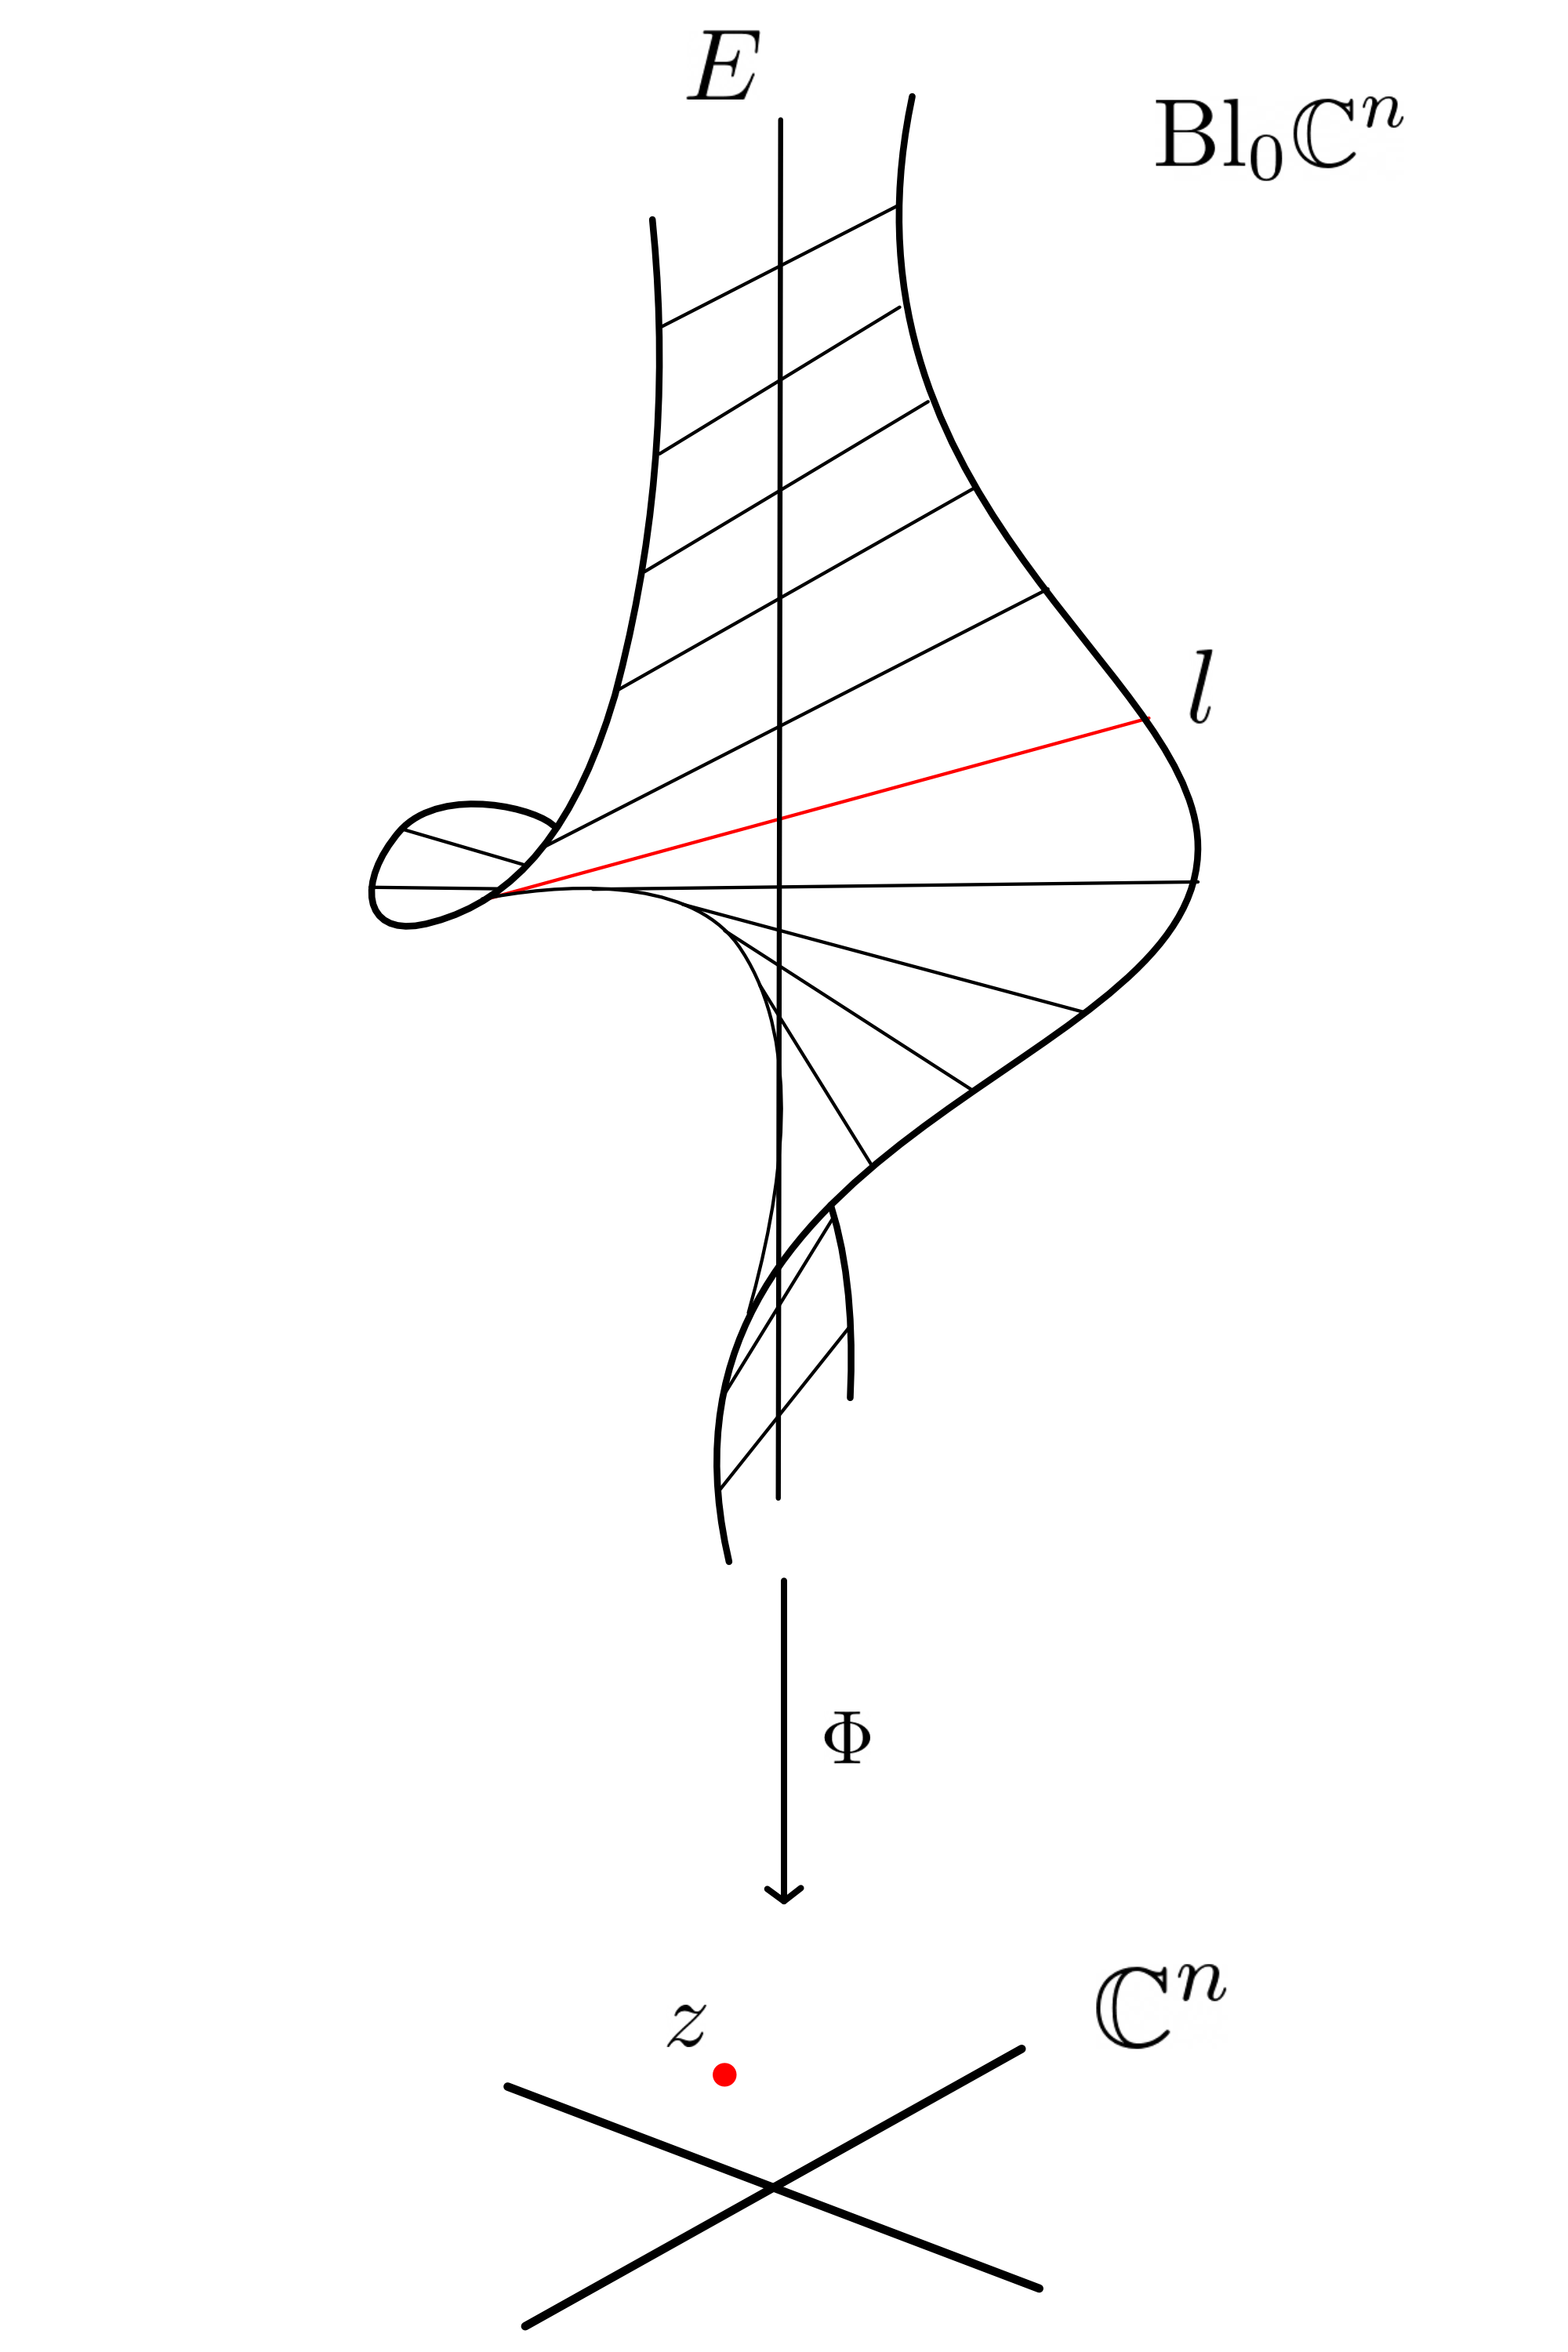
\includegraphics[width=0.45\linewidth]{Imagenes/exposion}
		\caption{Interpretación geométrica del blow-up}
		\label{fig:exposion}
	\end{figure}
	
\end{example}

Las modificaciones son los \enquote{morfismos elementales} de la geometría bimeromorfa, esto debido a que preservan las funciones meromorfas:

\begin{propo}\parencite[Chap VII, Sec. 1, Prop. 1.3]{grauertremment}
	Sea $\Phi:M\to N$ una modificación propia.
	\begin{enumerate}
		\item La aplicación canónica $\widehat{\Phi}:\oo_N\to \Phi_*(\oo_M)$ es un morfismo de gavillas inyectivo.
		\item La aplicación canónica $\widetilde{\Phi}:\mathscr{K}_N\to\Phi_*\mathscr{K}_M$ es un isomorfismo de gavillas.
	\end{enumerate}
	En particular, $\Phi$ induce un isomorfismo de campos $\mathscr{K}(M)\cong\mathscr{K}(N)$.
\end{propo}

\begin{definition}
	Sea $M$ y $N$ variedades complejas. Decimos que una aplicación
	\begin{equation*}
		f:M\dashrightarrow N
	\end{equation*}
	es dice \textbf{meromorfa} si cumple que
	\begin{enumerate}
		\item Existe un subconjunto analítico $A\subset M$ de codimensión al menos $1$ tal que $f$ está bien definido y holomorfo sobre el conjunto abierto denso $U=M\setminus A$. Este conjunto es llamado \textbf{conjunto de indeterminación}.
		\item La cerradura de la gráfica
		\begin{equation*}
			\Gamma_f := \{(x,y)\in U\times N : y=f(x)\}\subset M\times N
		\end{equation*}
		es una subvariedad analítica.
		\item La proyección a la primera coordenada $\Gamma_f\to M$ es una modificación propia.
	\end{enumerate}
	Decimos que $f$ es un \textbf{bimeromorfismo} si existe otra aplicación meromorfa $g:N\dashrightarrow M$ tal que
	\begin{align*}
		f\circ g= id_N,\\
		g\circ f= id_M.
	\end{align*}
	En este caso decimos que $M$ es \textbf{bimeromorfa} a $N$.
\end{definition}

Una aplicación meromorfa $f:M\dashrightarrow N$ puede interpretarse como una aplicación holomorfa después de resolver las indeterminaciones. Específicamente si tomamos las proyecciones
\begin{equation*}
	p_M:\Gamma_f\longrightarrow M\qquad\text{y}\qquad p_N:\Gamma_f\longrightarrow N
\end{equation*}
entonces
\begin{equation*}
	f=p_N\circ p_M^{-1}.
\end{equation*}
Es decir, $f$ se factoriza por una modificación propia. 

De esta manera, $f:N\dashrightarrow M$ es holomorfo casi en todas partes y su gráfica define un subvariedad analítica \enquote{bien comportada} en $M\times N$. La parte \enquote{meromorfa} consiste precisamente en permitir un conjunto de indeterminación de codimensión $\geq 1$, donde no hay una función bien definida.

\begin{remark}\parencite[Chap VII, Sec. 1]{grauertremment}
	Algunos hechos importantes de estas aplicaciones son los siguientes:
	\begin{enumerate}
		\item Si $L$ es un haz lineal sobre $M$, entonces la aplicación inducida
		\begin{equation*}
			\varphi_L:M\longrightarrow\pp^N
		\end{equation*}
		es una aplicación meromorfa, donde el conjunto de indeterminación es $Bs(L)$.
		\item (Teorema de eliminación de indeterminaciones) Sea $f:M\dashrightarrow N$ una aplicación meromorfa. Entonces existe una modificación propia $\sigma:\tilde{M}\to M$ y una aplicación holomorfa $\tau:\tilde{M}\to N$ tal que el siguiente diagrama conmuta
		\begin{center}
			\begin{tikzcd}
				& {\tilde{M}} & \\
				\\
				M && N
				\arrow["\sigma"', from=1-2, to=3-1]
				\arrow["\tau", from=1-2, to=3-3]
				\arrow["f"', from=3-1, to=3-3]
			\end{tikzcd}
		\end{center}
		\item Toda modificación propia es bimeromorfismo.
		\item Toda modificación propia $\Phi:M\to N$ entre superficies complejas compactas es la composición de una cantidad finita de blow-ups en un solo punto.
		\item Toda aplicación bimeromorfa $f:M\dashrightarrow N$ entre variedades complejas compactas puede escribirse como una composición $f=f_1\circ\cdots\circ f_k$ donde $f_i$ son blow-up en un punto o la inversa de un blow-ups en un punto. A la composición de un blow-up con su inversa suele ser llamado \textbf{transformación monoidal}.
	\end{enumerate}
\end{remark}

Análogo al caso de geometría algebraica, si $f:M\dashrightarrow N$ es una aplicación bimeromorfa, entonces induce un isomorfismo de campos
\begin{equation*}
	\mathcal{K}(N)\cong \mathcal{K}(M).
\end{equation*}
Eso significa que
\begin{equation*}
	a(N)=a(M).
\end{equation*}
Por lo tanto, la dimensión algebraica es un invariante bimeromorfo. 

\begin{theorem}[de Moishezon]\parencite{Moishezonlemmachow}
	Sea $M$ una variedad de Moishezon, entonces existe una aplicación bimeromorfa $f:M\dashrightarrow V$ donde $V$ es una variedad algebraica. Es decir, $M$ es bimeromorfa a una variedad algebraica.
\end{theorem}

Este teorema, con un sabor idéntico al \textit{lema de Chow}, muestra una naturaleza algebraica de ciertas variedades complejas. Además, orienta el estudio de la geometría compleja hacia la combinación de técnicas analíticas, birracionales y algebraicas. 

\begin{remark}\parencite[Chap. VII, Sec. 6.4]{grauertremment}\label{espaciosdemoishezon}
	Un \textbf{espacio complejo} (o espacio analítico complejo) es un espacio localmente anillado $(X,\oo_X)$ tal que $X$ es Hausdorff y para cada punto $x\in X$ existe una vecindad $U$ isomorfa a un subconjunto analítico abierto de $\cc^n$, es decir, el espacio localmente anillado $(U,\oo_X|_U)$ es isomorfo a espacio localmente anillado $(Y,\oo_Y)$ donde $Y$ es el abierto
	\begin{equation*}
		Y=\{x\in \Omega\subset\cc^n:f_1(x)=\cdots=f_k(x)=0\}
	\end{equation*}
	junto a la gavilla cociente definida por
	\begin{equation*}
		\oo_Y=\oo_\Omega/\langle f_1,\dots, f_k\rangle,
	\end{equation*}
	restringida a la topología de $Y$.
	
	Los espacios complejos generalizan a las variedades complejas, admitiendo singularidades y elementos nilpotentes en su gavilla. Más aún, existe un funtor llamado \textbf{funtor de analitificación}
	\begin{equation*}
		(\_)^{an}:\{\text{esquemas de tipo finito}/\cc\}\to\{\text{espacios analíticos complejos}\},
	\end{equation*}
	el cual le asocia a un esquema $X$ de tipo finito sobre $\cc$ un espacio complejo $X^{an}$. Sin embargo, este funtor no es una equivalencia pues, como hemos visto, existen muchas variedades complejas (o subconjuntos analíticos en general) que no son algebrizables. Un \textbf{espacio de Moishezon} $X$ es un espacio complejo compacto reducido (sin nilpotentes) bimeromorfo a una variedad algebraica, o equivalentemente,
	\begin{equation*}
		a(X)=\dim X.
	\end{equation*}
	Con lo cual, también hemos trabajado en determinar que espacios de Moishezon sí provienen de esquemas proyectivos de tipo finito sobre $\cc$. Por lo tanto, podemos también preguntarnos: ¿Cuáles son los \enquote{objetos algebraicos} que corresponden con espacios de Moishezon (si es que existen)?
	\end{remark}

\subsection{Variedades de Kähler}

En geometría compleja, la geometría diferencial se desarrolla bajo la restricción impuesta por la estructura compleja. El análogo complejo de una métrica riemanniana es una métrica hermitiana, que es compatible con la estructura compleja y permite introducir nociones métricas respetando la holomorfía. Entre ellas, las métricas de Kähler se distinguen por satisfacer una condición diferencial que unifica la geometría riemanniana, simpléctica y compleja, dando lugar a una teoría especialmente rígida y estructurada.

Para trabajar en este contexto diferencial, primero debemos presentar los espacios tangentes a una variedad compleja. Las construcciones están principalmente basadas de los libros \parencite[Sec. 1.2]{huybrechts2005complex} y \parencite[Cap. 1]{leecomplex}. Fijemos $M$ una variedad compleja y $p\in M$. 
\begin{equation*}
	T_{\rr,p}M=\mathrm{gen}_\rr\left\{\frac{\partial}{\partial x_i},\frac{\partial}{\partial y_i}\right\}.
\end{equation*} 
Definamos el endomorfismo
\begin{align*}
	&J:T_{\rr,p}M\longrightarrow T_{\rr,p}M\\
	J\left(\frac{\partial}{\partial x_i}  \right)&=\frac{\partial}{\partial y_i},\qquad J\left(\frac{\partial}{\partial y_i} \right)=-\frac{\partial}{\partial x_i},
\end{align*}
el cual cumple que $J^2=-\mathrm{Id}$. Esta función es llamada \textbf{estructura casi compleja} de $T_{\rr,p}M$. Ahora, consideremos el espacio complexificado
\begin{equation*}
	T_{\cc.p}M=T_{\rr,p}M\otimes \cc,
\end{equation*}
el cual es llamado \textbf{espacio tangente complejo} de $p$. Además, podemos considerar la extensión de la estructura casi compleja al espacio complexificado $J_\cc:T_{\cc.p}M\to T_{\cc.p}M$. De esta manera, tenemos la descomposición
\begin{equation*}
	T_{\cc.p}M=T_{p}^\prime M\oplus T_p^{\prime\prime}M, 
\end{equation*}
donde
\begin{align*}
	&T_{p}^\prime M=\{v\in T_{\cc.p}M: J(v)=iv\},\\		&T_p^{\prime\prime}M =\{v\in T_{\cc.p}M: J(v)=-iv\}.
\end{align*}
En particular, el espacio $T_{p}^\prime M$ es llamado \textbf{espacio tangente holomorfo} y juega el papel del espacio tangente en la geometría compleja. Además, se cumple que
\begin{equation*}
	\dim_{\cc} T_{p}^\prime M=n
\end{equation*}
pues los operadores 
\begin{equation*}
	\frac{\partial }{\partial z_i}=\frac{1}{2}\left( \frac{\partial }{\partial x_i}-i\frac{\partial }{\partial y_i}\right).
\end{equation*}
forman una base para el espacio tangente holomorfo. Más aún, se tiene la siguiente sucesión exacta de $\rr$-módulos
\begin{center}
	\begin{tikzcd}
		0 & {T_{\mathbb{R},p}M} & {T_{\mathbb{C},p}M} & {T_p^\prime M} & 0
		\arrow[from=1-1, to=1-2]
		\arrow[from=1-2, to=1-3]
		\arrow[from=1-3, to=1-4]
		\arrow[from=1-4, to=1-5]
	\end{tikzcd}
\end{center}
Por lo tanto, podemos concluir que
\begin{equation*}
	T_{\mathbb{R},p}M\cong T_p^\prime M
\end{equation*}
\begin{definition}
	Una \textbf{forma hermitiana} es una función $h:T^\prime_pM\times T^\prime_pM\to\cc$ lineal en la primera entrada y 
	\begin{equation*}
		h(v_1,v_2)=\overline{h(v_2,v_1)},\qquad v_1,v_2\in T^\prime_pM.
	\end{equation*}
\end{definition}
De la definición podemos notar es $\cc$-antilineal y $h_p(v,v)\in\rr$ para todo $v\in T^\prime_pM$. Decimos que $h_p$ es \textbf{positiva definida} si $h_p(v,v)>0$ para todo $v\in T^\prime_pM$.

Usando el isomorfismo $T_{\rr,p}M\cong T^\prime_pM$, podemos ver que si $h_p$ es positivo definido se cumple que
\begin{equation*}
	g(v_1,v_2):=\mathrm{Re}h_p(v_1,v_2)=\frac{1}{2}(h_p(v_1,v_2)+h_p(v_2,v_1))
\end{equation*}
es una métrica riemanniana sobre $M$ como variedad suave. Más aún, $h_p$ está definida únicamente por $g_p$.

\begin{definition}
	Una función bilineal $g:T^\prime_pM\times T^\prime_pM\to\rr$ sobre $M$ se dice \textbf{compatible} con $J$ si
	\begin{equation*}
		g(Ju,Jv)=g(u,v),\qquad\text{para todo }u,v\in T_pM.
	\end{equation*}
\end{definition}

Notemos que la estructura casi compleja $J$ actúa como una rotación $90^\circ$ en cada plano complejo del espacio tangente, pero una métrica albitraria no necesariamente respeta este giro. La compatiblidad de $g$ nos dice que medir después de girar por $J$ es lo mismo que girar después de medir. Un cálculo directo muestra que:
\begin{propo}
	Una función $h_p:T^\prime_pM\times T^\prime_pM\to\cc$ es forma hermitiana si, y solo si, $g_p=\mathrm{Re}h_p$ es una métrica riemanniana en $p$ compatible con $J$.
\end{propo}
%\begin{proof}
%	Supongamos que $h_p:T^\prime_pM\times T^\prime_pM\to\cc$ es una forma hermitiana. Definimos $g:T_{\rr,p}M\times T_{\rr,p}M\to\rr$ la función dada por
%	\begin{equation*}
%		g(v_1,v_2)=\mathrm{Re}h_p(v_1,v_2)=\frac{1}{2}(h_p(v_1,v_2)+h_p(v_2,v_1)).
%	\end{equation*}
%	Notemos que $g$ es bilineal, pues
%	\begin{align*}
%		g(\lambda v_1+v_2,v)=\frac{1}{2}(h_p(\lambda v_1+v_2,v)+h_p(v,\lambda v_1+v_2))=\frac12 (\lambda h_p(v_1,v)+h_p(v_2,v)+\overline{\lambda}\overline{h_p(v_1,v)}´+\overline{h_p(v_1,v)})
%	\end{align*}
%	\textcolor{red}{ACABAR EJEMPLO}
%\end{proof}

Esto significa que la forma hermitiana $h_p$ determina de manera única una métrica riemanniana compatible con $J$, y viceversa. 

Considerando la parte imaginaria
\begin{equation*}
	w_p(u,v)=-\mathrm{Im}h_p(u,v)=\frac{i}{2}(h_p(u,v)-h_p(v,u))
\end{equation*}
es una forma bilineal alternante tal que $w_p(u,v)=g_p(u,Jv)$. Más aún, $h_p$ está definida únicamente por $w_p$.

\begin{propo}
	Una función $h_p:T^\prime_pM\times T^\prime_pM\to\cc$ es forma hermitiana si, y solo si, $w_p=-\mathrm{Im}h_p$ es una 2-forma compatible con $J$.	
\end{propo}
%\begin{proof}
%	\textcolor{red}{FALTA DEMOSTRACIÓN}
%\end{proof}

\begin{definition} 
	Una métrica hermitiana $H$ sobre una variedad compleja $M$ es una colección de formas Hermitianas $h_p$ para todo punto $p\in M$.
\end{definition}

De esta manera, una métrica hermitiana $H$ induce una métrica riemanniana $g=\mathrm{Re}H$ y una $2$-forma diferencial real valuada $w=-\mathrm{Im}H$. A esta forma diferencial se le llamada \textbf{forma fundamental} de $H$. Por lo tanto, esta métrica se puede interpretarse como la versión mínima y natural de una métrica riemanniana que respeta la estructura casi compleja.

\begin{propo}
	Toda variedad compleja admite una métrica hermitiana.
\end{propo}
\begin{proof}
	Sea $M$ una variedad compleja y consideremos una métrica riemanniana $g_0$ arbitraria. Definamos otra métrica riemanniana
	\begin{equation*}
		g(u,v)=g_0(u,v)+g_0(Ju,Jv).
	\end{equation*}  
	Notemos que
	\begin{equation*}
		g(Ju,Jv)=g_0(Ju,Jv)+g_0(J^2u,J^2v)=g_0(-u,-v)+g_0(Ju,Jv)=g_0(u,v)+g_0(Ju,Jv)=g(u,v).
	\end{equation*}
	De esta manera, $g$ es compatible con $J$. Por lo tanto, definiendo $w(u,v)=g(u,Jv)$ obtenemos una métrica hermitiana para $M$
	\begin{equation*}
		h(u,v)=g(u,v)-iw(u,v).
	\end{equation*}
\end{proof}                                     

Si $M$ tiene coordenadas $(z^1,\cdots,z^n)$, entonces una dos forma diferencial $\omega$ está dada por
\begin{equation*}
	\omega=\sum_{i<j}w_{ij}(z)dz^i\wedge dz^j,
\end{equation*}
entonces
\begin{equation*}
	d\omega=\sum_{i<j<k}\left( \frac{\partial w_{jk}}{\partial z_i}+\frac{\partial w_{ki}}{\partial z_j}+\frac{\partial w_{ij}}{\partial z_k}\right)dz^i\wedge dz^j\wedge dz^k.
\end{equation*}
Decimos que $w$ es cerrada si $d\omega=0$.

\begin{definition}
	Una \textbf{variedad de Kähler} es una variedad compleja equipada con una métrica Hermitiana $H$ cuya forma fundamental $\omega=-\mathrm{Im}H$ es cerrada, esto es,
	\begin{equation*}
		d\omega=0.
	\end{equation*}
	En este caso, la forma fundamental $w$ es llamada \textbf{forma de Kähler}.
\end{definition}

La forma fundamental $w$ puede interpretarse como una medida de áreas compatibles con la estructura compleja, por lo que pedir que sea cerrada nos dice que esas áreas complejas no varían infinitesimalmente al moverse en la variedad. Así, la métrica $g$ y la forma $w$ nos respetan los ángulos y áreas a un nivel complejo, es decir, son compatibles con la estructura compleja tanto desde el punto de vista métrico como simpléctico.

Veamos ahora unos ejemplos importantes de variedades de Kähler, los cuales nos ayudarán a entender el caso de algebrización.

\begin{example}
	Consideremos $\cc^n$ con la métrica donde $\frac{\partial}{\partial z_j}$ forman una base unitaria. La estructura casi compleja $J$ actúa sobre los vectores tangentes como
	\begin{equation*}
		J\frac{\partial}{\partial x_j}=\frac{\partial}{\partial y_j},\quad
		J\frac{\partial}{\partial y_j}=-\frac{\partial}{\partial x_j}.
	\end{equation*}
	La métrica euclidiana estándar en $\mathbb{C}^n\simeq\mathbb{R}^{2n}$ es
	\begin{equation*}
		g=\sum_{j=1}^n (dx_j\otimes dx_j+dy_j\otimes dy_j).
	\end{equation*}
	Por otro lado,
	\begin{equation*}
		\omega(u,v)=g(u,Jv).
	\end{equation*}
	En coordenadas, usando que $J$ envía $\partial/\partial x_j\mapsto\partial/\partial y_j$, se obtiene
	\begin{equation*}
		\omega=\sum_{j=1}^n dx_j\wedge dy_j=\frac{i}{2}\sum_{j=1}^{n} dz_i\wedge d\overline{z}_j.
	\end{equation*}
	Como $\omega$ tiene coeficientes constantes, su diferencial exterior es
	\begin{equation*}
		d\omega=\sum_{j=1}^n d(dx_j\wedge dy_j)=
		\sum_{j=1}^n (d dx_j)\wedge dy_j - dx_j\wedge d dy_j=0,
	\end{equation*}
	porque $d (dx_j)=d (dy_j)=0$ para diferenciales exactos de coordenadas. Así que
	\begin{equation*}
		d\omega=0\quad\text{en todo}\qquad \mathbb{C}^n.
	\end{equation*}
	Por lo tanto, $\cc^n$ es una variedad de Kähler.
\end{example}

\begin{example}
	Sea $N\subset M$ una subvariedad compleja. Para todo $p\in N$ se cumple que $T_p^\prime N\subset T_p^\prime M$, entonces una métrica Hermitiana $H_M$ induce naturalmente una métrica en $N$. Calculando en coordenadas locales, se cumple que
	\begin{equation*}
		w_N=i^*w_M
	\end{equation*}
	donde $i:N\hookrightarrow M$ es la aplicación inclusión. Por lo tanto, si $M$ es de Kähler, entonces $N$ también lo es.
\end{example}

\begin{example}[Métrica de Fubini-Study]
	Consideremos el $n$-espacio proyectivo $\pp^n$ y la carta afín
	\begin{equation*}
		U_0=\{[Z_0:\cdots:Z_n]:Z_0\neq 0\}\subset\pp^n.
	\end{equation*}
	con coordenadas locales
	\begin{equation*}
		z_i=\frac{Z_i}{Z_0}.
	\end{equation*} 
	Definamos la función
	\begin{equation*}
		\varphi(z)=\log(1+\|z\|^2)=\log(1+|z_1|^2+\cdots+|z_n|^2).
	\end{equation*}
	llamada \textbf{potencial de Kähler} de la forma 
	\begin{equation*}
		\omega_{FS}=\frac{i}{2\pi}\partial \overline{\partial}\varphi.
	\end{equation*}
	La métrica hermitiana está dada por
	\begin{equation*}
		h_p\left(\frac{\partial}{\partial z_i},\frac{\partial}{\partial z_j}\right)=\frac{\partial^2 \varphi}{\partial z_i\partial \overline{z}_j}=\frac{(1+\|z\|^2)\delta_{ij}-\overline{z}_i z_j}{(1+\|z\|^2)^2}.
	\end{equation*}
	Por las identidades de Dolbeault,
	\begin{equation*}
		\partial^2=\overline{\partial}^2=0,\qquad d=\partial+\overline{\partial}.
	\end{equation*}
	tenemos que
	\begin{equation*}
		d\omega_{FS}=\frac{i}{2\pi}(\partial+\overline{\partial})\partial \overline{\partial}\varphi=\frac{i}{2\pi}(\partial^2\overline{\partial}\varphi+\overline{\partial}\partial\overline{\partial}\varphi)=0.
	\end{equation*}
	Por lo tanto, $\omega_{FS}$ es una forma de Kähler llamada \textbf{forma fundamental de Fubini-Study}.
\end{example}

Como las variedades algebraicas son subvariedades complejas de un espacio proyectivo (véase ejemplo \ref{algsonsubvariedades}), los dos últimos ejemplos implican que todas las variedades algebraicas son variedades de Kähler. Por lo tanto:

\begin{corollary}
	Toda variedad compleja algebrizable es de Kähler.
\end{corollary}

En la teoría de Hodge, se estudia la cohomología de las variedades de Kähler y con una consecuencia de la descomposición de Hodge se llega a la conclusión de que las superficies de Hopf no son de Kähler (véase  \parencite[Corollary 6.13]{2002hodge}). De esta manera, no todas las variedades complejas son de Kähler ni es una condición suficiente para ser algebrizable. 

Una pregunta que nos hicimos en la sección anterior fue ¿Toda variedad de Moishezon es algebrizable? Vimos que si hay algún contraejemplo, debe estar en dimensión $\geq 3$. Vamos a construir el \textit{contraejemplo de Hironaka} que es una variedad de Moishezon de dimensión 3 que no es de Kähler, y en consecuencia tampoco es algebrizable. Para entender este ejemplo, vamos a utilizar un hecho importante de las variedades de Kähler:

\begin{theorem}\label{integralpositiva}
	Sea $M$ una variedad compleja compacta, entonces forma de Kähler $w$ en $M$ se evalúa positivamente sobre cualquier curva compleja irreducible $C\subset M$, es decir,
	\begin{equation*}
		\int_C w>0.
	\end{equation*}
\end{theorem}

\begin{example}[Contraejemplo de Hironoka]\label{hironakaejemplo}\parencite{barlet2015exampleshhironaka}
	Sea $X$ una variedad algebraica no singular de dimensión $3$, por ejemplo podemos tomar $X=\pp^3$. Consideremos dos curvas no singulares $C_1, C_2\subset X$ que se intersectan transversalmente en exactamente dos puntos
	\begin{equation*}
		P,Q\in X.
	\end{equation*} 
	Entonces podemos cubrir a $X$ por dos abiertos
	\begin{equation*}
		X=(X\setminus P)\cup(X\setminus Q).
	\end{equation*}
	Con esto, los puntos $P$ y $Q$ quedan separados por cada abierto. En cada abierto, vamos a hacer dos blow-up: En $X\setminus P$ hacemos un blow-up con centro en $C_1$ y luego hacemos blow-up en la preimagen propia de la curva $C_2$. Análogamente, en $X\setminus Q$ hacemos un blow-up con centro en $C_2$ y luego hacemos blow-up en la preimagen propia de la curva $C_1$.\\
	Como $C_1$ y $C_2$ no se intersectan en $(X\setminus P)\cap(X\setminus Q)$, los dos espacios obtenidos son isomorfos en la intersección y se pueden pegar. Así, obtenemos una variedad compleja $\tilde{X}$ y un bimeromorfismo propio
	\begin{equation*}
		\pi:\tilde{X}\longrightarrow X.
	\end{equation*} 
	Así, $X$ es bimeromorfa a $\tilde{X}$ y $\tilde{X}$ es de Moishezon, pues $X$ lo es. El contraejemplo consiste en demostrar que $\tilde{X}$ no admite métrica de Kähler.\\
	Sea 
	\begin{align*}
		L_1=\pi^{-1}(x),\qquad \text{ con }x\text{ punto genérico de }\enspace C_1.\\
		L_2=\pi^{-1}(y),\qquad \text{ con }y\text{ punto genérico de }\enspace C_2.
	\end{align*}
	Entonces
	\begin{equation*}
		L_1\cong \pp^1,\qquad L_2\cong\pp^1,
	\end{equation*}
	pues son fibras excepcionales de blow-up de curvas en una $3$-variedad. Ahora, la fibra de $\pi$ en $Q$ se descompone en dos componentes irreducibles
	\begin{equation*}
		\pi^{-1}(Q)=L_1^\prime\cup L_2^\prime,
	\end{equation*}
	donde $L_1^\prime$ proviene del blow-up a lo largo de $C_1$ y $L_2^\prime$ proviene del blow-up a lo largo de $C_2$. Además, se tienen las siguientes relaciones homológicas
	\begin{align*}
		&L_1^\prime\sim L_1\\
		&L_2^\prime\sim L_2\\
		&L_1^\prime+L_2^\prime\sim L_1
	\end{align*}
	Análogamente en $P$ obtenemos la descomposición $\pi^{-1}(P)=L_1^{\prime\prime}\cup L_2^{\prime\prime}$ con las relaciones
	\begin{align*}
		&L_1^{\prime\prime}\sim L_1\\
		&L_2^{\prime\prime}\sim L_2\\
		&L_1^{\prime\prime}+L_2^{\prime\prime}\sim L_2
	\end{align*}
	Así, obtenemos que
	\begin{equation*}
		L_1^\prime+	L_2^\prime\sim 0\qquad\text{en}\enspace H_2(\tilde{X},\zz).
	\end{equation*}	
	Si $\tilde{X}$ admitiera una forma de Kähler $w$, entonces por el teorema \ref{integralpositiva} tendríamos que
	\begin{equation*}
		\int_{L^\prime_1} w >0,\qquad	\int_{L^\prime_2} w >0.
	\end{equation*}
	Luego
	\begin{equation*}
		\int_{L^\prime_1+L^\prime_2} w>0.
	\end{equation*}
	Sin embargo, como el ciclo $L_1^\prime+	L_2^\prime$ es homológicamente trivial entonces $\int_{L_1^\prime+L_2^\prime}w=0$, lo cual es una contradicción. Por lo tanto, $\tilde{X}$ no admite métricas de Kähler. En consecuencia, $\tilde{X}$ tampoco puede ser algebrizable.
	\begin{figure}[H]
		\centering
		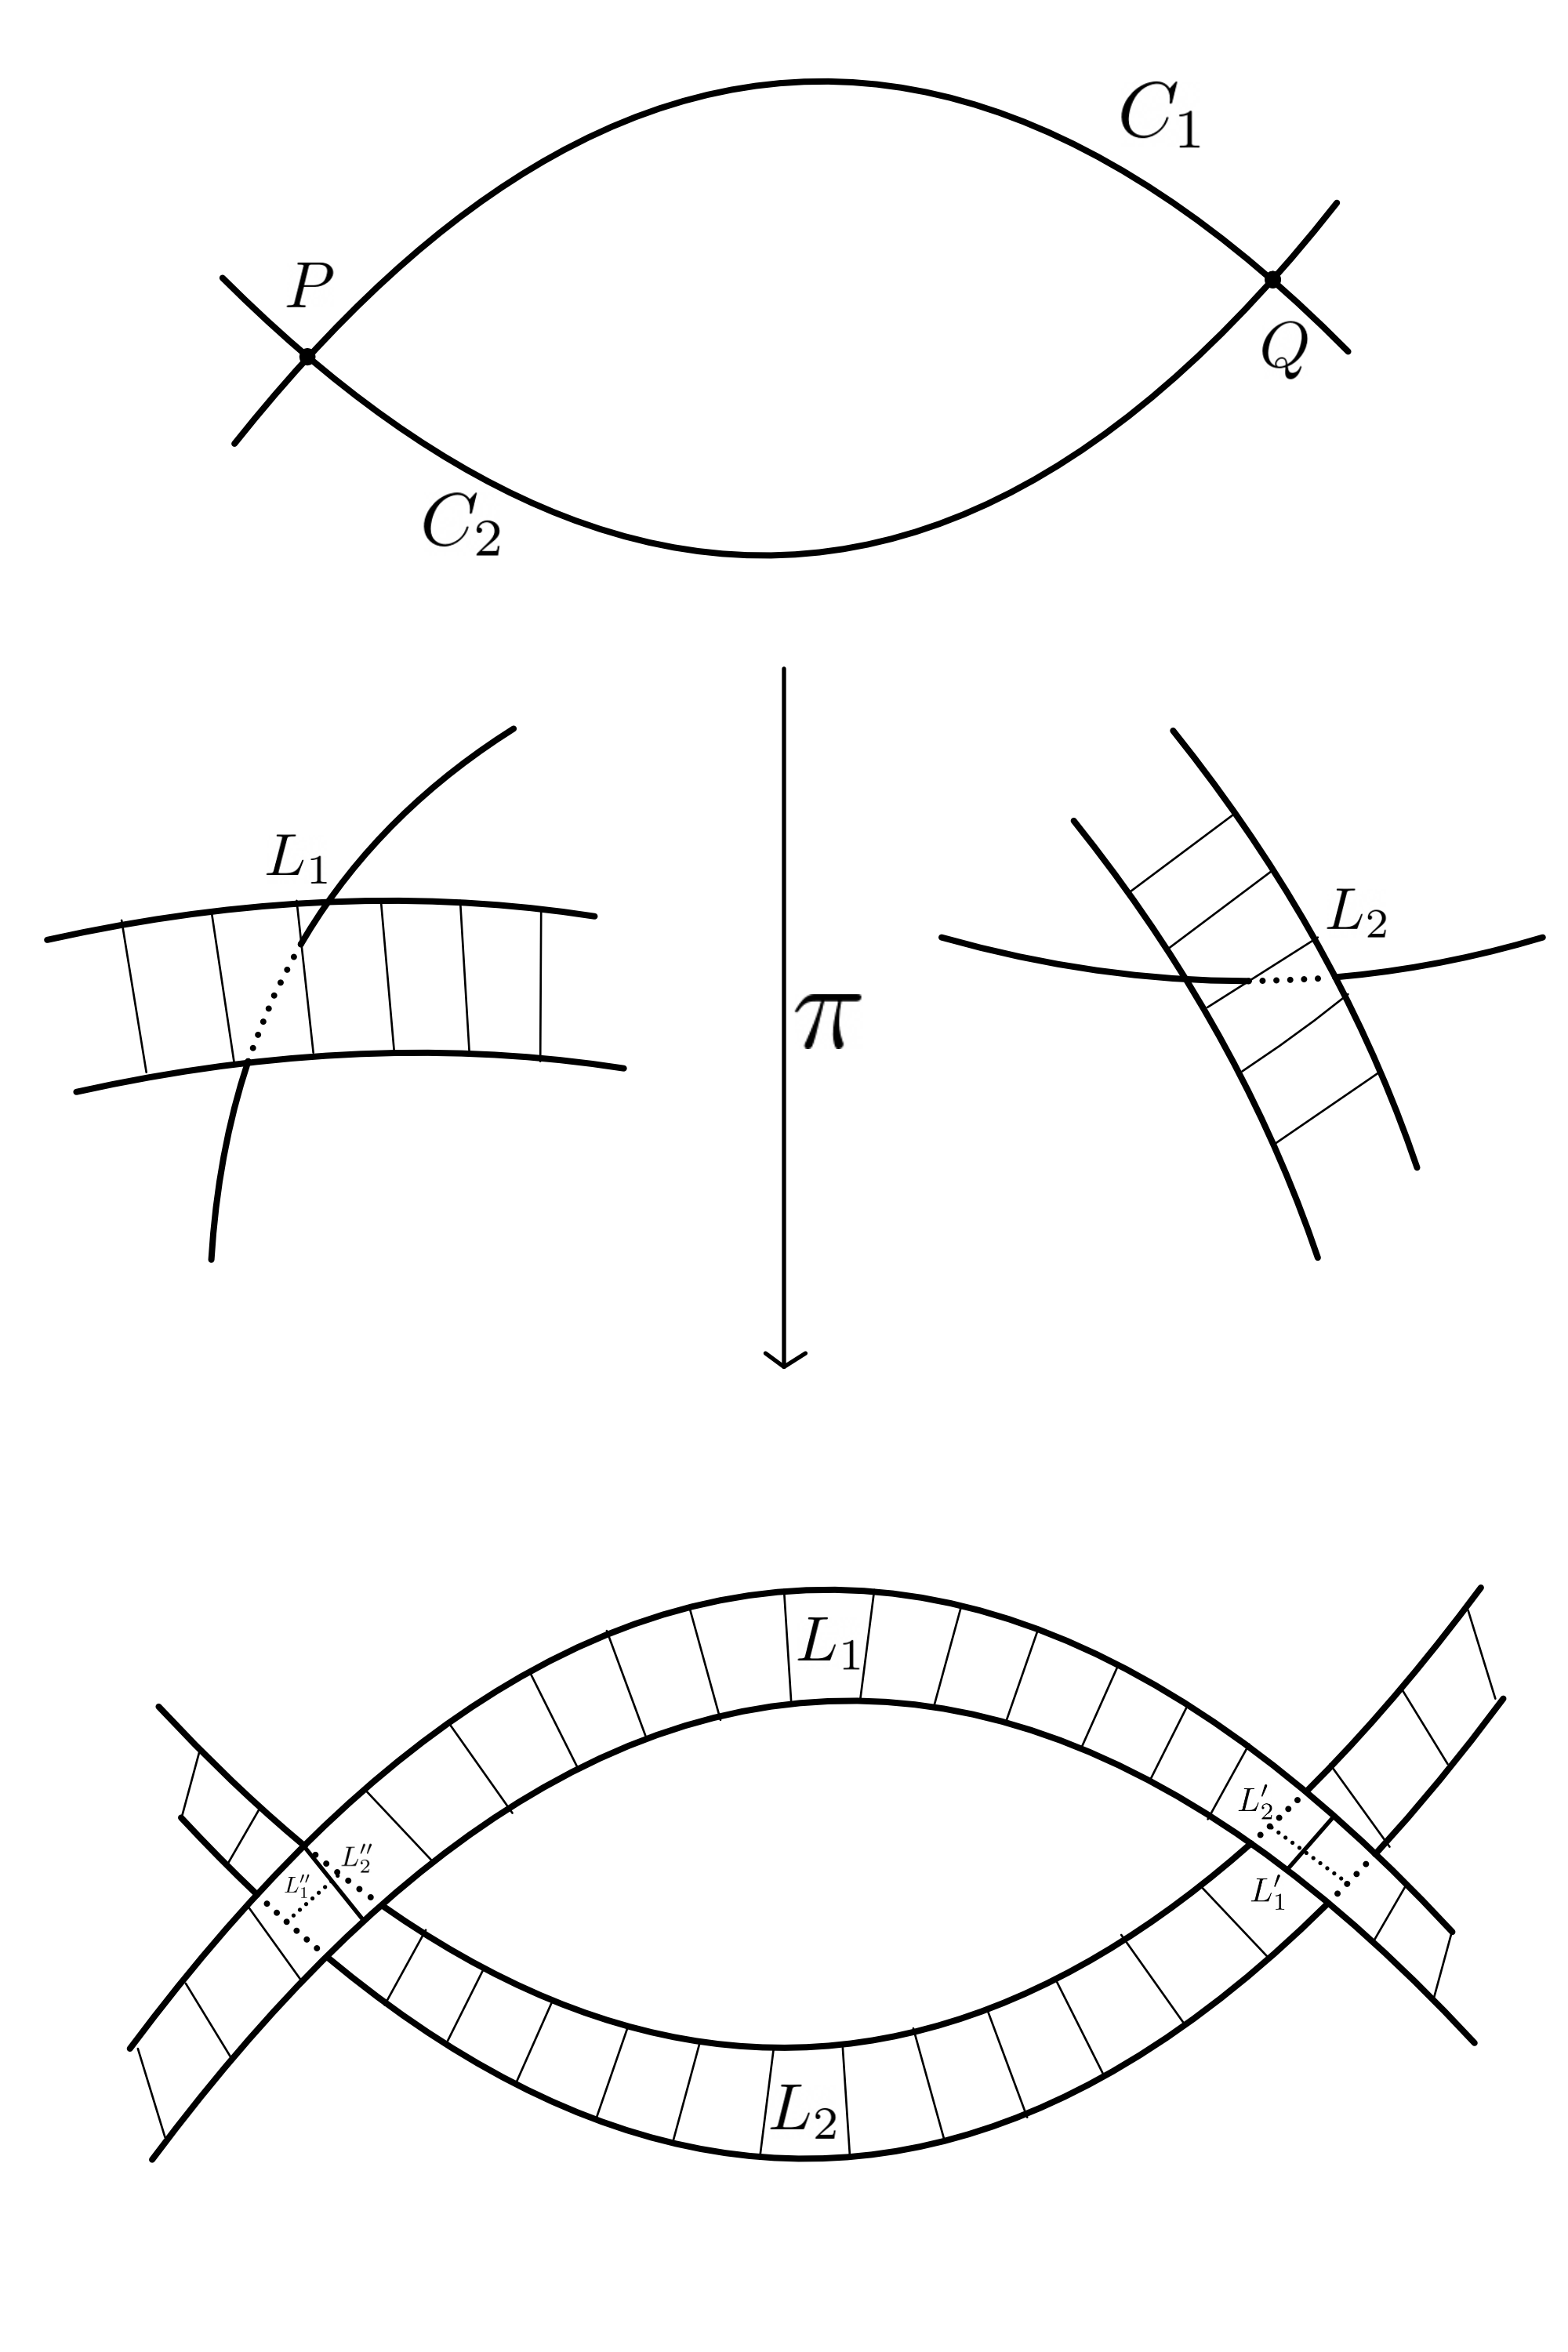
\includegraphics[width=0.4\linewidth]{Imagenes/Ejemplo Hironaka}
		\caption{Contraejemplo de Hironaka}
		\label{fig:ejemplo-hironaka}
	\end{figure}
\end{example}

\begin{remark}\parencite[Chap. VII, Sec. 6.4]{grauertremment}
	Continuando la observación \ref{espaciosdemoishezon}. El matemático americano \textit{Michael Artin} desarrolló unos objetos llamados \textbf{espacios algebraicos}. Intuitivamente, en lugar de utilizar esquemas afines como piezas locales de esquemas, los puntos en un espacio algebraico solo tienen vecindades étale y estas \enquote{piezas étale} luego deben pegarse. Los esquemas son naturalmente espacio algebraicos, pero una observación importante es que el contraejemplo de Hironaka genera un espacio algebraico que no es esquema. Además, se puede extender el funtor de analitificación al funtor
	\begin{equation*}
		(\_)^{an}:\{\text{espacios algebraicos de tipo finito }/\cc\}\longrightarrow\{\text{espacios complejos}\}.
	\end{equation*}
	En particular, Artin probó que este funtor induce la equivalencia categórica
	\begin{equation*}
		\{\text{espacios algebraicos propios de tipo finito}/\cc\}\cong\{\text{espacios de Moishezon}\}.
	\end{equation*}
	En otras palabras, todo espacio de Moishezon es de manera única un espacio algebraico, es decir, los espacios de Moishezon no se pueden pegar en general con la topología de Zariski como los esquemas, pero sí con la topología étale. Concluyendo que, para las necesidades de la geometría bimeromorfa, la categoría de esquemas suele ser insuficiente pues hay muy pocos objetos. Pero la categoría de espacios algebraicos sí lo es: no se puede abandonar esta categoría mediante modificaciones. 
\end{remark}

El resultado más importante de esta sección y conclusión final es el otro teorema demostrado por Moishezon.

\begin{theorem}[Teorema fundamental de Moishezon]\parencite{Moishezon1967}\label{fundamentaldemoishezon}
	Toda variedad de Moishezon y Kähler es algebrizable.
\end{theorem}

Este resultado conecta de forma conclusiva las distintas áreas de la geometría, pues significa que condiciones algebraicas y diferenciables en un contexto complejo imponen una estructura algebraica. De este modo, el teorema nos muestra la interacción entre la geometría diferencial, a través de la existencia de métricas de Kähler, y la geometría algebraica mediante la dimensión algebraica, dentro del marco de la geometría compleja, concluyen de manera natural al problema de algebrización abordado durante todo este trabajo. 

	
	%-----------------------new page----------------------------
	
%	\chapter*{Conclusiones}
\addcontentsline{toc}{chapter}{Conclusiones}

Las variedades algebraicas tienen una estructura bastante rígida pero, al mismo tiempo, bien comprendida en la geometría algebraica clásica. En contraste, las variedades complejas, aunque son más restrictivas que las variedades diferenciables reales, admiten una amplia gama de comportamientos globales. Por ejemplo, existen superficies complejas que no poseen funciones meromorfas no constantes (véase el ejemplo \ref{hopfsuperficie}), así como variedades complejas que no admiten métricas de Kähler (véase el contraejemplo de Hironaka \ref{hironakaejemplo}). Estos fenómenos nos muestran que las variedades complejas son mucho más diversas que las algebraicas, y en consecuencia, determinar si una variedad compleja es algebrizable y describir explícitamente las ecuaciones algebraicas que la definen, es una tarea lejos de ser trivial.

La algebrización de variedades complejas es un tema bastante profundo que admite múltiples enfoques. Por un lado, el teorema fundamental de Moishezon \ref{fundamentaldemoishezon} establece que una variedad compleja compacta es algebraica si, y solo si, es de Moishezon y de Kähler. Este resultado muestra claramente que la algebrización requiere al mismo tiempo de riqueza algebraica, medida mediante con la dimensión algebraica, y una riqueza geométrica, expresada mediante la existencia de una métrica de Kähler.

%Por otro lado, en este trabajo abordamos el problema de algebraización construyendo directa y explícitamente un encaje holomorfo de una variedad compleja compacta en un espacio proyectivo. Con esto conseguimos llevar toda la variedad, por medio de un biholomorfismo, al espacio proyectivo sin aplastarla o deformarla, es decir, preservando fielmente su estructura compleja. Adicionalmente, con el teorema de la aplicación propia (falta cita), esta incrustación termina siendo una subvariedad analítica del espacio proyectivo, concluyendo así por el teorema de Chow (falta cita) que nuestra variedad compleja es de hecho algebraica.

Por otro lado, en este trabajo abordamos el problema de algebraización construyendo directa y explícitamente un encaje holomorfo de una variedad compleja compacta en un espacio proyectivo. Con esto conseguimos llevar toda la variedad, por medio de un biholomorfismo, al espacio proyectivo sin aplastarla o deformarla, es decir, preservando fielmente su estructura compleja. Adicionalmente, con el teorema de la aplicación propia \ref{aplicacionpropia}, este encaje determina termina siendo una subvariedad analítica del espacio proyectivo, lo que nos conduce al teorema de Chow. Este resultado nos afirma que los subconjuntos analíticos del espacio proyectivo son conjuntos algebraicos, es decir, se pueden describir como conjuntos de ceros de una cantidad finita de polinomios homogéneos. De esta manera, concluimos que toda variedad compleja que admite un encaje holomorfo en un espacio proyectivo es algebrizable.

Además, en nuestra búsqueda de los encajes al proyectivo, encontramos que los haces lineales juegan un papel fundamental, ya que inducen una aplicación holomorfa a un espacio proyectivo con una base del espacio de secciones globales. Los haces lineales que inducen un encaje son llamados haces amplios, y así, concluimos que una variedad compleja es algebraica si, y solo si, admite un haz amplio (véase teorema \ref{proyectivossiamplio}). Como consecuencias, obtuvimos que toda superficie de Riemann es algebraica. Asimismo, ejemplificamos cómo la teoría de curvas elípticas permite describir explícitamente el toro complejo como una curva algebraica proyectiva. Finalmente, construimos explícitamente una realización algebraica de la variedad compleja $\mathbb P^1\times\mathbb P^1$, junto con la ecuación proyectiva que la describe.

Durante todo el trabajo observamos que el estudio de variedades complejas no puede abordarse de manera aislada, requiere interactuar con diversas áreas de las matemáticas. Por ejemplo, fue esencial comprender las propiedades básicas de las variedades algebraicas, estudiar la geometría local compleja y considerar el contexto clásico de las superficies de Riemann, cuya teoría en dimensión uno ilustra la profundidad y riqueza de la teoría general.

En esencia, la algebrización consiste en demostrar que la estructura analítica de una variedad compleja es suficientemente rica para reconstruirse a partir de objetos algebraicos. Esta tesis tiene como objetivo explicar y detallar el proceso de algebrización de variedades complejas. Para ello, se desarrolla un método de construir explícitamente encajes holomorfos al espacio proyectivo a través de haces lineales, y se detalla por qué esto es suficiente para que una variedad compleja admita una estructura algebraica. Esto motiva naturalmente la búsqueda y el estudio de condiciones que garanticen la existencia de haces amplios. Además, vimos la algebrización conecta directamente con resultados más profundos como los teoremas de Moishezon. Esta interacción entre geometría compleja y geometría algebraica constituye una de las ideas centrales desarrolladas a lo largo de este trabajo. Por lo tanto, el trabajo puede servir de base para futuras investigaciones sobre la interacción entre geometría compleja y geometría algebraica, ofreciendo una base sólida para explorar tópicos más avanzados en esta dirección.

%	En general, una variedad algebraica no está determinada necesariamente como puntos en un espacio proyectivo, por ejemplo una variedad $X$ definida como un esquema reducido separable de tipo finito sobre $\cc$. En esta caso, podemos obtener el espacio de puntos complejos $X(\cc)$, los cuales tienen la estructura topológica necesaria para obtener una variedad compleja \parencite{shafarevich2016basic}. 
%
%\begin{definition}
%	Sea $X$ una variedad algebraica sobre $\cc$. La \textbf{analiticación} de $X$, denotada por $X^{an}$, es la variedad compleja obtenida al considerar el conjunto de puntos complejos $X(\mathbb{C})$ dotado de la topología compleja y su estructura natural de variedad compleja.
%\end{definition}
%
%En general, se define el funtor
%\begin{equation*}
%	(-)^{an} : \mathrm{Var}*{\mathbb{C}} \longrightarrow \mathrm{Var}*{\mathbb{C}}^{an},
%\end{equation*}
%de la categoría de variedades algebraicas sobre $\cc$ a la categoría de variedades complejas\footnote{En general, a la categoría de espacios complejos \parencite{shafarevich2016basic}.}.
	
	
	
	%-----------------------new page----------------------------
	
%	\appendix
%	
%	\chapter*{Apéndice}
\addcontentsline{toc}{chapter}{Apéndice}

\setcounter{section}{0}
\renewcommand{\thesection}{A.\arabic{section}}

\section{Funciones holomorfas de varias variables}

No es objetivo indagar demasiado en el estudio de las funciones complejas en varias variables. Sin embargo, es necesario presentar el concepto de holomorfia para definir una variedad compleja. La mayoria de resultados se pueden encontrar en \parencite[Cap 1, Sec 1.1]{huybrechts2005complex}\\
Fijemos $U\subset\cc^n$ un subconjunto abierto. Para cualquier $w\in U$, definimos el \textbf{polidisco} como el conjunto definido por
\begin{equation*}
	B_\epsilon(w):=\{z: |z_i-w_i|<\epsilon_i\},\enspace \text{donde}\enspace \epsilon=(\epsilon_1,\epsilon_2,\cdots,\epsilon_n)
\end{equation*}

\begin{definition}[Función holomorfa]\label{taylor}
	Una función $f:U\subset \cc^n\to\cc$ es llamada holomorfa en un punto $w\in U$, si existe un polidisco $B_\epsilon(w)\subset U$ tal que la restricción $f\left.\right|_{B_\epsilon(w)}$ está dada por una serie de potencias convergente \begin{equation*}
		\sum_{(i_1,i_2,\cdots,i_n)\in\nn^n}^{\infty}a_{i_1,i_2,\cdots,i_n}(z_1-w_1)^{i_1}(z_2-w_2)^{i_2}\dots(z_n-w_n)^{i_n}
	\end{equation*}
	y es única.
\end{definition}

\begin{remark}[Definiciones equivalentes de holomorfia] Sea $f:U\to\cc$ una función. Entonces $f$ es holomorfa si 
	\begin{enumerate}
		\item Satisface las ecuaciones de Cauchy-Riemann en todas las coordenadas $z_j=x_j+iy_j$, es decir,
		\begin{equation*}
			\frac{\partial f}{\partial \overline{z_j}}=0,\qquad j=1,2,\cdots n
		\end{equation*}
		donde $\frac{\partial}{\partial \overline{z_j}}=\frac{1}{2}(\frac{\partial}{x}+i\frac{\partial }{\partial y})$.
		
		\item Es continuamente diferenciable y para todo $z\in U$ se cumple la siguiente fórmula
		\begin{equation*}
			f(z)=\frac{1}{(2\pi i)^n}\int_{\partial B_\epsilon(w)}\frac{f(w)}{(z_1-w_1)\dots(z_n-w_n)}dw_1\cdots dw_n
		\end{equation*}
	\end{enumerate}
	
\end{remark}

Veamos las generalizaciones de los resultados básico en una variable.

\begin{theorem}[Principio del máximo]\label{Principiodelmodulomaximo}
	Sea $U\subset \cc^n$ un conjunto abierto y conexo. Si $f:U\to\cc$ es una función holomorfa no constante, entonces $|f|$ no tiene un máximo local en $U$.
\end{theorem}

\begin{theorem}[de la identidad]\label{identidad}
	Sea $U\subset \cc^n$ un subconjunto abierto y conexo. Si $f,g:U\to \cc$ son funciones holomorfas tales que $f(z)=g(z)$ para todo $z$ es un abierto no vacio de $U$, entonces $f=g$.
\end{theorem}

\begin{theorem}[de Lioville]
	Toda función $f:\cc^n\to\cc$ holomorfa acotada es constante.  
\end{theorem}

\begin{theorem}[Hartogs]\label{hartogs}
	Sea $\Omega\subset\cc^n$ con $n\geq 2$ un dominio y $K\subset\Omega$ un subconjunto compacto tal que $\Omega\setminus K$ es también conexo. Entonces, toda función holomorfa $f:\Omega\setminus K\to\cc$ se extiende holomorfamente a todo $\Omega.$
\end{theorem}


\begin{definition}\label{mapholocn}
	Una función $f:U\to\cc^m$ es llamada \textbf{aplicación holomorfa} si todas las funciones coordenadas $f_1,\dots,f_m:U\to\cc$ son funciones holomorfas.
\end{definition}


\begin{definition}
	Sean $U,V\subset \cc^n$ dos abiertos no vacios. Un aplicación holomorfa $f:U\to V$ es \textbf{biholomorfa} si es biyectiva y su inversa $f^{-1}$ también es una aplicación holomorfa. Además decimos que $U$ y $V$ son biholomorfos. 
\end{definition}

El caso del teorema del mapeo de Riemann es un caso que no se puede extender a más dimensiones y es exclusivo para $n=1$.
\begin{theorem}
	Sea $B_1^n(0)=\{z\in\cc^n: \|z\|<1\}$ la bola euclidiana unitaria y $P_1^n(0)=\{z\in\cc^n:|z_i|<1,\text{ para cada }i=1,2,\cdots, n\}$ el polidisco unitario en $\cc^n$. Entonces $B_1^n(0)$ y $P_1^n(0)$ son biholomorfos si, y solo si, $n=1$. La demostración se encuentra en \parencite[Teo 3.9, Pg. 78]{scheidemann}
\end{theorem}


\begin{definition}\label{puntoregular}
	Sean $U\subset \cc^m$ un conjunto abierto y $f:U\to\cc^n$ una aplicación holomorfa. El \textbf{jacobiano} (complejo) de $f$ en un punto $z\in U$ es la matriz 
	\begin{equation*}
		J(f)(z):=\left(\frac{\partial f_i}{\partial z_j}(z) \right)_{i,j}
	\end{equation*}
	Un punto $z\in U$ es llamado \textbf{regular} si el rango de la matriz jacobiana $J(f)(z)$ es $n$. Si todo punto $z\in f^{-1}(w)$ es regular, decimos que $w$ es un \textbf{valor regular}.
\end{definition}



\begin{theorem}[Teorema de la función inversa]
	Sea $f:U\to V$ una aplicación holomorfa entre dos subconjuntos abiertos $U,V\subset \cc^n$ y $z\in U$. Entonces los siguiente enunciados son equivalentes:
	\begin{enumerate}
		\item $\det J(f)(z)\neq 0$
		\item Existen vecindades $z\in U'\subset U$ y $f(z)\in V'\subset V$ tal que 
		\begin{equation*}
			f\left.\right|_{U'}:U'\to V'
		\end{equation*}
		es un biholomorfismo.
	\end{enumerate}
\end{theorem}

\begin{theorem}[Teorema de la función implícita]\label{funcionimplicita}
	Sea $U\subset\cc^{n+m}$ un abierto y $f:U\to \cc^n$ una aplicación holomorfa en $U$. Si $(w_0,z_0)\in U$ es un punto tal que
	$$ \det\left(\frac{\partial f_i}{\partial z_j}(w_0,z_0)\right)_{1\leq i,j \leq n}\neq 0$$
	Entonces existe una vecindad $W\subset \cc^m$ de $w_0$, una vecindad de $Z\subset\cc^n$ de $z_0$ y una aplicación holomorfa $g:W\to Z$ tal que $f(w,g(w))=0$ para todo $w\in W$ y
	\begin{equation*}
		\{(w,z)\in U':f(w,z)=0\}=\{(w,g(w))\in U:w\in W\}
	\end{equation*}
\end{theorem}



\begin{propo}\label{biholomorfismojac}
	Sea $f:U\to V$ una aplicación holomorfa biyectiva entre dos subconjuntos abiertos $U,V\subset \cc^n$. Entonces para todo $z\in U$ se tiene que $\det J(f)(z)\neq 0$. En particular, $f$ es un biholomorfismo.
\end{propo}

\section{Comportamiento local}\label{complocal}
	
	En una variable compleja, el comportamiento local de las funciones holomorfas es muy simple. Si $f:U\to\cc$ es una función holomorfa en alguna vecindad $U\subset\cc$ del cero, entonces $f$ se escribe de forma única como
	\begin{equation*}
		f(z)=u(z)z^k
	\end{equation*} 
	para algún $k\in\nn$ y una función $u\in\mathscr{O}_n(U)$ unidad. Esto significa que $u(0)\neq 0$ y $1/u(z)$ está bien definida en alguna vecindad del cero. En varias variables complejas la situación es mucho más complicada.\\
	\begin{definition}
		Sean $U,V\subset \cc^n$ vecindades del $0\in\cc^n$. Decimos que $f\in\mathscr{O}_n(U)$ y $g\in\mathscr{O}_n(V)$ están relacionadas si existe una vecindad $W\subset\cc^n$ del $0$ tal que
		\begin{equation*}
			f|_{U\cap W}=g|_{V\cap W}
		\end{equation*} 
		Llamamos a la clase de equivalencia $[f]$ \textbf{germen} de la función $f$ en el cero.
		Denotamos por $\oo_{n}$ al conjunto de gérmenes de funciones en el cero.
	\end{definition}
	
	\begin{remark}
		Si $f,g\in \oo_{n}$ son gérmenes, entonces podemos definir las operaciones
		\begin{align*}
			[f]+[g]:=[f+g]\\
			[f][g]:=[fg].
		\end{align*}
		Por lo tanto, el conjunto $\oo_{n}$ es un anillo. Más aún, $\cc$ está contenido en $\oo_{n}$ a travez de las funciones constantes y este anillo puede ser descrito por el límite directo
		\begin{equation*}
			\oo_{n}=\lim_{0\in U}\oo_n(U).
		\end{equation*} 
	\end{remark}
	
	Nosotros podemos pensar a un germen $[f]\in\oo_{n}$ como una función holomorfa alrededor del cero en alguna vecidad no especificada. Más aún, el valor $f(0)\in\cc$ está bien definido para gérmenes, pero no está bien definidido para cualquier otro punto.\\
	
	\begin{remark}
		Por definición, una función $f$ es holomorfa en $0\in\cc^n$ si puede ser expandido como una serie de potencias convergente 
		\begin{equation*}
			f(z)=\sum_{\alpha\in\nn}a_\alpha z^\alpha.
		\end{equation*}
		De está manera, tenemos un isomorfismo de anillos 
		\begin{equation*}
			\oo_{n}\cong \cc\{z_1,\cdots,z_n\}
		\end{equation*}
		donde $\cc\{z_1,\cdots,z_n\}$ es el anillo de series convergentes (alrededor del cero) en las variables $z_1,\cdots,z_n$.
	\end{remark}

	\begin{example}
		Para $n=0$, tenemos que $\oo_{n}\cong\cc$. Para $n=1$, se cumple que $\oo_{n}\cong\cc\{z\}$. Así, las funciones holomorfas alrededor del cero en una variable corresponden algebraicamente con el anillo $\cc\{z\}$. Este anillo es un anillo de valuación discreta, esto es, todo ideal de $\cc\{z\}$ es de la forma $\langle z^k \rangle$ para algún $k\in\nn$.
	\end{example}
	
	De esta manera, estudiar el comportamiento local de las funciones holomorfas es equivalente a estudiar las propiedades algebraicas del anillo $\oo_{n}$.
	
	\begin{remark}[$\oo_{n}$ es un anillo local]
		Consideremos el conjunto de elementos no invertibles en $\oo_{n}$
		\begin{equation*}
			\mathfrak{m}_n=\{f\in\oo_{n}:f(0)=0\}.
		\end{equation*}
		Ya que si $f(0)\neq 0$, entonces $1/f$ es holomorfa en una vecindad alrededor del origen. Así, $1/f\in\oo_{n}$. Más aún, $\mathfrak{m}_n$ es un ideal pues si $f\in\oo_{n}$ y $m\in\mathfrak{m}_n$, entonces $(fm)(0)=0$. Con esto $fm\in\oo_{n}$, es decir, $\mathfrak{m}_n$ es un ideal de $\oo_{n}$. Esto significa que $\oo_{n}$ es un anillo local.\\
		En particular, si $f\in\mathfrak{m}_n\subset \cc\{z_1,\cdots,z_n\}$ entonces su expansión en serie no tiene coeficiente independiente
		\begin{equation*}
			f=\sum_{\alpha\in\nn^n\setminus\{0\}}a_\alpha z^{\alpha}.
		\end{equation*}
		Esto significa que el ideal $\mathfrak{m}_n$ es finitamente generado y
		\begin{equation*}
			\mathfrak{m}_n=\langle z_1,\dots,z_n \rangle.
		\end{equation*}
	\end{remark}
	Notemos que el campo residual $\oo_{N}/\mathfrak{m}_n$ es isomorfo a $\cc$. En particular, el entero $n$ (la dimensión de $\cc^n$) se puede recuperar del anillo local $\oo_{n}$. Dado que el ideal maximal $\mathfrak{m}_n$ está generado por lo elementos $z_1,\dots,z_n$, entonces imagen de los generadores bajo el cociente
	\[\begin{tikzcd}
		{\mathfrak{m}_n} && {\mathfrak{m}_n/\mathfrak{m}_n^2}
		\arrow["\rho", from=1-1, to=1-3]
	\end{tikzcd}\]
	genera una base para $\mathfrak{m}_n/\mathfrak{m}_n^2$. Por lo que:
	\begin{corollary}
		El cociente $\mathfrak{m}_n/\mathfrak{m}_n^2$ es un $\cc$-espacio vectorial de dimensión $n$.
	\end{corollary}
	
	Otra propiedad importante y simple de demostrar de este anillo es el siguiente resultado.
	
	\begin{propo}
		El anillo $\oo_{n}$ es un dominio entero.
	\end{propo}
	
	Este anillo tiene propiedades aún más profundas e importantes, pero tenemos que estudiar la estructura local de las funciones holomorfas con más cuidado. Notemos que tenemos una inclusión natural de anillos 
	\begin{equation*}
		\oo_{n-1}\subset \oo_{n-1}[z_n]\subset \oo_n.
	\end{equation*}
	Los elementos del anillo $\oo_{n-1}[z_n]$ son polinomios de la forma $z_n^k+a_1z_n^{k-1}+\cdots+a_k$ con $a_1,\dots,a_k\in \oo_{n-1}$, los cuales son gérmenes en $\oo_n$. Además, la primera inclusión tiene una naturaleza algebraica mientras que la segunda es más analítica. Ahora vamos a presentar el resultado fundamental para entender esta segunda inclusión llamado \textit{Teorema de Preparación de Weierstraß}.
	
	\begin{definition}
		Un elemento $z_n^k+a_1z_n^{k-1}+\cdots+a_k\in\oo_{n-1}[z_n]$ con $k\geq 1$ es llamado \textbf{polinomio de Weierstraß} si $a_1,\dots,a_k\in \mathfrak{m}_{n-1}$.
	\end{definition}
		Análogamente al caso de una varieable, queremos ver como esencialmente todo germen $f\in\oo_n$ puede ser escrito de la forma $f=uh$ donde $h$ es un polinomio de Weierstraß y $u$ es unidad. Sin embargo, como $h(0,z_n)=z_n^d$, tenemos que si $f=uh$ entonces $f$ restringida a la línea $w=(z_1,\dots,z_{n-1})$ no puede ser identicamente cero.  
	\begin{definition}
		Sea $U\subset\cc^n$ una vecindad del cero y $f\in\oo_n(U)$. Decimos $f$ es \textbf{regular} en $z_n$ si la función holomorfa $f(0,z_n)$ no es identicamente cero. Además, como $f(0,z_n)=u(z_n)z_n^d$ para algún $d$, decimos que $f$ es regular de \textbf{orden} $d$.
	\end{definition}
		La notación de regularidad tiene sentido para los elementos de $\oo_n$ ya que solo depende del comportamiento de $f$ en alguna vecindad albitrariamente pequeña del origen.
		
	\begin{theorem}[Teorema de Preparación de Weierstraß]
		Si $f\in\oo_n$ es regular de orden $d$ en $z_n$, entonces existe un único polinomio de Weierstraß $h\in\oo_{n-1}[z_n]$ de grado $d$ tal que $f=uh$ para alguna unidad $u\in\oo_n$.
	\end{theorem}
		La idea de la demostración es un poco simple: Fijando $w\in\cc^{n-1}$ suficientemente cerca del origen, y consideremos $f_w(z_n):=f(w,z_n)$ la cual es una función holomorfa en $z_n$. Ya que $f_0(z_n)$ tiene un cero de orden $d$, entonces cada $f_w(z_n)$ tiene exactamente $d$ ceros (contando sus multiplicidades) cerca del origen. Escribimos como $a_1(w),\dots,a_d(w)$ las raíces y se define la función $u_w(z_n)=(z_n-a_1(w))\cdots(z_n-a_d(w))$. El objetivo principal de la prueba es demostrar que la función $h=f_w(z_n)/u_w(z_n)$ es holomorfa en $w$.\\
		La prueba formal y completa se puede consultar en \parencite[Cap. 1, Sec, 1.1, Prop. 1.1.6]{huybrechts2005complex}.
		
	\begin{propo}\label{anillodfu}
		El anillo $\oo_{n}$ es un dominio de factorización única.
	\end{propo}
	
	Existe una manera de hacer división larga de polinomios de Weierstraß, al igual que el anillo $\cc[z]$ y este resultado también es fundamental sobre el álgebra local.
	
	\begin{theorem}[Teorema de división de Weierstraß]
		Sea $h\in\oo_{n-1}[z_n]$ un polinomio de Weierstraß de grado $d$. Entonces para todo $f\in\oo_n$ puede ser escrito de manera única de la forma
		\begin{equation*}
			f=qh+r,\qquad\text{para }q\in \oo_n 
		\end{equation*} 
		y $r\in\oo_{n-1}[z_n]$ es un polinomio de grado $<d$. Más aún. si $f\in\oo_{n-1}[z_n]$, entonces también $q\in\oo_{n-1}[z_n]$.
	\end{theorem}
	\begin{proof}
		\parencite[Cap. 1, Sec, 1.1, Prop. 1.1.17]{huybrechts2005complex}
	\end{proof}
	
	De esta manera tenemos nuestra última propiedad importante del anillo de gérmenes de funciones holomorfas.
	
	\begin{theorem}\label{anillonoetheriano}
		El anillo $\oo_{n}$ es un anillo Noetheriano.
	\end{theorem}
	\begin{proof}
		Vamos a probar el teorema por indución sobre $n$. El caso para $n=0$ es trivial, pues el anillo $\oo_n=\cc$ es noetheriano.\\
		Supongamos que $\oo_{n-1}$ es un anillo noetheriano. Entonces por el teorema de la base de Hilbert, el anillo de polinomios $\oo_{n-1}[z_1]$ es noetheriano. Sea $I\subset\oo_n$ un ideal no cero y tomemos $0\neq f\in I$. Haciendo un cambio de coordenadas de ser necesario, podemos aplicar el teorema de Preparación de Weierstraß a $f$, es decir, existe un polinomio de Weierstraß $g\in \oo_{n-1}[z_1]$ y $h\in\oo_n$ unidad tal que
		\begin{equation*}
			f=gh.
		\end{equation*}
		En particular, $g\in I$. Luego, el ideal $I\cap \oo_{n-1}[z_1]$ es finitamente generado en $\oo_{n-1}[z_1]$, digamos
		\begin{equation*}
			I\cap \oo_{n-1}[z_1]=\langle g_1,\dots,g_k \rangle.
		\end{equation*}
		Para cualquier otro $\tilde{f}\in I$, el teorema de división de Weierstraß nos dice que 
		\begin{equation*}
			\tilde{f}=g\tilde{h}+r
		\end{equation*}
		para algún $r\in\oo_{n-1}[z_1]$. Más aún, como $\tilde{f},g,\tilde{h}\in I$, también $r\in I$ y podemos concluir que $r\in I\cap \oo_{n-1}[z_1]$. De esta manera,
		\begin{equation*}
			\tilde{f}=g\tilde{h}+\sum_{i=1}^{k}a_ig_i.
		\end{equation*}
		Por lo tanto, $I$ está generado por los elementos $\{g,g_1,\dots,g_k\}$.
	\end{proof}
	
	
\section{Álgebra de los conjuntos analíticos}
	
		Usaremos todas las propiedades algebraicas del anillo local $\oo_n$ para describir el álgebra y la geometría los conjuntos analíticos en $\cc^n$. En primer lugar, definamos una relación de equivalencia sobre subconjuntos de $\cc^n$.
	\begin{definition}
			Sean $X,Y\subset \cc^n$ y $a\in X\cap Y$.
			\begin{enumerate}
				\item Decimos  que $X$ y $Y$ son \textbf{equivalentes en} $a$ si existe una vecindad abierta $U$ de $a$ tal que
				\begin{equation*}
					X\cap U = Y\cap U.
				\end{equation*}
				\item Una clase de equivalencia de $X$ es  llamada \textbf{germen} de $X$ en $a$, y es denotada por
				\begin{equation*}
					[X_a].
				\end{equation*}
				Se omite el punto $a$ cuando el punto es fijo o claro.
				\item Si $[X]$ y $[Y]$ son gérmenes de conjuntos, definimos
				\begin{align*}
					[X]\cap[Y]&:=[X\cap Y]\\
					[X]\cup[Y]&:=[X\cup Y]\\
					[X]\subset[Y]&:\Longleftrightarrow [X]\cap[Y]=[X].
				\end{align*}
				\item Si $[f]\in\oo_0$ es representado por algún $f\in\oo(U)$ donde $U\subset\cc^n$ es alguna vecindad de origen, definimos
				\begin{equation}
					Z([f]):=[Z(f)].
				\end{equation}
				\item [5. ]Si $[X_0]$ es un germen del cero y $[f]\in\oo_0$, decimos que $[f]$ se anula en $[X]$ si
				\begin{equation*}
					[X]\subset Z([f]).
				\end{equation*}
			\end{enumerate}
	\end{definition}

	Nos centraremos en estudiar conjuntos analíticos solo en el origen, por lo que el concepto de germen es necesario para solo conservar su información alrededor del origen.
	
	\begin{definition}
			Un germen $[X]$ es llamado \textbf{germen analítico} o \textbf{conjunto analítico} si existe una cantidad finita de gérmenes de funciones holomorfas $[f_1],\cdots,[f_k]\in\oo_0$ tal que
			\begin{equation*}
				[X]=Z([f_1],\cdots,[f_k])
			\end{equation*}
	\end{definition}
		
	\begin{propo}
			Si $[X]$ y $[Y]$  son gérmenes analíticos,  entonces $[X]\cap [Y]$ y $[X]\cup [Y]$ también son gérmenes analíticos.
	\end{propo}
	
		\begin{definition}
			Sea $[X]$ un germen analítico en el cero y $A\subset\oo_n$. Definimos
			\begin{equation*}
				I([X]):=\{[f]\in\oo_0:[X]\subset Z([f])\}
			\end{equation*}
			y
			\begin{equation*}
				Z(A)=\bigcap_{[f]\in A}Z([f]).
			\end{equation*}
		\end{definition}
		
	\begin{example}
		Calculando el $I$ del germen del conjunto $\{0\}$,
		\begin{align*}
			I([\{0\}])&=\{[f]\in\oo_0:[f]\text{ se anula  en }[\{0\}]\}\\
			&=\{f\text{ holomorfa en el cero}:f(0)=0\}\\
			&=\mathfrak{m}_n,
		\end{align*}
		el cual es el ideal maximal de $\oo_0$.
		Ahora, calculando los ceros de todo el anillo $\oo_0$,
		\begin{equation*}
			Z(\oo_n)=\bigcap_{[f]\in\oo_0}Z([f])=\emptyset
		\end{equation*}
		ya que $\oo_0$ contiene las constantes.
	\end{example}
	
	
	\begin{propo} $ $
		\begin{enumerate}
			\item El conjunto $I([X])$ es un ideal del anillo $\oo_n$, llamado \textbf{ideal asociado}.
			\item El conjunto $Z(A)=Z(\langle A\rangle)$ es  un germen analítico.
		\end{enumerate}
	\end{propo}
	
	\begin{propo}
		Sea $[X]$ un germen analítico. Entonces
		\begin{equation*}
			Z(I([X]))=[X].
		\end{equation*}
	\end{propo}
	
	\begin{theorem}[de Rückert]
		Sea $\mathfrak{a}\subset\oo_0$ cualquier ideal. Entonces
		\begin{equation*}
				I(Z([\mathfrak{a}]))=\sqrt{\mathfrak{a}}.
		\end{equation*}
	\end{theorem}
	
	\begin{remark}
		Consideremos un ideal radical $J\subset\oo_0$, entonces existe un ideal $\mathfrak{a}\subset\oo_0$ tal que
		\begin{equation*}
			J=\sqrt{\mathfrak{a}}
		\end{equation*}
		Luego, por el teorema de Rückert
		\begin{align*}
			I(Z(J))=\sqrt{J}=\sqrt{\sqrt{\mathfrak{a}}}=\sqrt{\mathfrak{a}}=J
		\end{align*}
		Esto nos da una relación biyectiva entre los dos conjuntos
		\begin{align*}
			\begin{Bmatrix}
				\text{Gérmenes analíticos}\\
				\text{de }\cc^n
			\end{Bmatrix}\longleftrightarrow\begin{Bmatrix}
				\text{Ideales radicales}\\
				\text{de }\cc\{z_1,\dots,z_n\}
			\end{Bmatrix}
		\end{align*}
		Más aún, tenemos la relación
		\begin{align*}
			\begin{Bmatrix}
				\text{Gérmenes analíticos}\\
				\text{irreducibles de }\cc^n
			\end{Bmatrix}\longleftrightarrow\begin{Bmatrix}
				\text{Ideales primos}\\
				\text{de }\cc\{z_1,\dots,z_n\}
			\end{Bmatrix}
		\end{align*}
	\end{remark}
	
	\begin{definition}
		Sea $X$ un conjunto analítico irreducible definido por un ideal primo $\mathfrak{p}\subset\oo_n$. Definimos la \textbf{dimensión} de $X$ como
		\begin{equation*}
			\dim X:=\mathrm{dim}_{\text{krull}}\oo_n/\mathfrak{p}.
		\end{equation*}
		Además, definimos la \textbf{codimensión} de $X$ como $\mathrm{codim}X:=n-\dim X$.
	\end{definition}
	
	Sea $X\subset\cc^n$ un germen analítico irreducible de codimensión $1$, es decir, $\dim X=n-1$. Entonces el ideal primo $\mathfrak{p}$ asociado a $X$ tiene altura $1$ en $\oo_n$. Un resultado esencial de los DFU es que todo ideal de altura $1$ es principal. Esto significa que 
	\begin{equation*}
		\mathfrak{p}=\langle f \rangle 
	\end{equation*}
	para algún elemento irreducible $f\in\oo_n$. Por lo tanto, un germen analítico irreducible de codimensión uno está definido por una función holomorfa irreducible.
	
	\begin{propo}\label{hipersuperficiesenCn}
		Todo germen analítico irreducible de codimension uno es el conjunto de ceros de una sola función holomorfa irreducible.
	\end{propo}

	
	
	%-----------------------new page----------------------------
	
	\backmatter
	
	\nocite{*}
	\printbibliography[
	heading=bibnumbered,
	title={Referencias}
	]
	
	%-----------------------new page----------------------------
	
\end{document}
